\documentclass{book}
\usepackage[a4paper,top=2.5cm,bottom=2.5cm,left=2.5cm,right=2.5cm]{geometry}
\usepackage{makeidx}
\usepackage{natbib}
\usepackage{graphicx}
\usepackage{multicol}
\usepackage{float}
\usepackage{listings}
\usepackage{color}
\usepackage{ifthen}
\usepackage[table]{xcolor}
\usepackage{textcomp}
\usepackage{alltt}
\usepackage{ifpdf}
\ifpdf
\usepackage[pdftex,
            pagebackref=true,
            colorlinks=true,
            linkcolor=blue,
            unicode
           ]{hyperref}
\else
\usepackage[ps2pdf,
            pagebackref=true,
            colorlinks=true,
            linkcolor=blue,
            unicode
           ]{hyperref}
\usepackage{pspicture}
\fi
\usepackage[utf8]{inputenc}
\usepackage{mathptmx}
\usepackage[scaled=.90]{helvet}
\usepackage{courier}
\usepackage{sectsty}
\usepackage{amssymb}
\usepackage[titles]{tocloft}
\usepackage{doxygen}
\lstset{language=C++,inputencoding=utf8,basicstyle=\footnotesize,breaklines=true,breakatwhitespace=true,tabsize=8,numbers=left }
\makeindex
\setcounter{tocdepth}{3}
\renewcommand{\footrulewidth}{0.4pt}
\renewcommand{\familydefault}{\sfdefault}
\hfuzz=15pt
\setlength{\emergencystretch}{15pt}
\hbadness=750
\tolerance=750
\begin{document}
\hypersetup{pageanchor=false,citecolor=blue}
\begin{titlepage}
\vspace*{7cm}
\begin{center}
{\Large Key\-Cpp -\/-\/ A M\-A\-T\-L\-A\-B-\/like library for C++ }\\
\vspace*{1cm}
{\large Generated by Doxygen 1.8.3.1}\\
\vspace*{0.5cm}
{\small Mon Oct 21 2013 15:59:32}\\
\end{center}
\end{titlepage}
\clearemptydoublepage
\pagenumbering{roman}
\tableofcontents
\clearemptydoublepage
\pagenumbering{arabic}
\hypersetup{pageanchor=true,citecolor=blue}
\chapter{Key\-Cpp}
\label{index}\hypertarget{index}{}\section*{Download Source}

Right now you must download the source by cloning the git repository from \href{http://code.google.com/p/keycpp/source/checkout}{\tt code.\-google.\-com/p/keycpp/}. In the future as the library matures, there will be a compressed file to download and possibly a package for Debian/\-Ubuntu.

\subsection*{Dependencies}

Currently this project makes use of the \href{http://www.sourceforge.net/projects/kissfft/}{\tt Kiss F\-F\-T} and \href{http://code.google.com/p/gnuplot-cpp/}{\tt gnuplot-\/cpp} open source projects as well as the \href{http://www.netlib.org/lapack/}{\tt L\-A\-P\-A\-C\-K} libraries, \href{http://www.gnuplot.info/}{\tt Gnuplot} plotting program, and the \href{http://www.boost.org/doc/libs/1_54_0/libs/numeric/odeint/doc/html/index.html}{\tt Boost odeint} library. The sources from \href{http://www.sourceforge.net/projects/kissfft/}{\tt Kiss F\-F\-T} and \href{http://code.google.com/p/gnuplot-cpp/}{\tt gnuplot-\/cpp} have been incorporated into this project.

The {\itshape only} extra dependencies that you need on your system are the \href{http://www.netlib.org/lapack/}{\tt L\-A\-P\-A\-C\-K} libraries, \href{http://www.gnuplot.info/}{\tt Gnuplot}, and the \href{http://www.boost.org/doc/libs/1_54_0/libs/numeric/odeint/doc/html/index.html}{\tt Boost odeint} library.

\subsubsection*{Ubuntu (and various \href{https://wiki.ubuntu.com/UbuntuFlavors}{\tt flavors})}

To acquire all the required dependencies you can execute the following commands\-:

{\ttfamily sudo apt-\/get install build-\/essential}

Until Ubuntu 13.\-10 comes out in October 2013, you need to install \href{http://headmyshoulder.github.io/odeint-v2/}{\tt odeint} from their website. The way I did it was to install Boost (see below) and then copy the odeint header and source files into the appropriate Boost folders. This is because odeint first appears in Boost 1.\-53 and the newest version in the repository for Ubuntu 13.\-04 is 1.\-49.

{\ttfamily sudo apt-\/get install libboost-\/all-\/dev}

{\ttfamily sudo apt-\/get install libblas3gf libblas-\/doc libblas-\/dev}

{\ttfamily sudo apt-\/get install liblapack3gf liblapack-\/doc liblapack-\/dev}

\subsubsection*{Other Operating Systems}

Your mileage may vary.

\subsection*{Installation \& Usage}

{\itshape This library uses features only available in the \href{https://en.wikipedia.org/wiki/C%2B%2B11}{\tt C++11 standard}. Y\-O\-U M\-U\-S\-T \href{http://gcc.gnu.org/projects/cxx0x.html}{\tt C\-O\-M\-P\-I\-L\-E} W\-I\-T\-H T\-H\-I\-S S\-T\-A\-N\-D\-A\-R\-D.}

To install Key\-Cpp onto your system first clone the git repository to a directory of your choice\-: {\ttfamily git clone \href{https://code.google.com/p/keycpp/}{\tt https\-://code.\-google.\-com/p/keycpp/}}

The following command will compile the Key\-Cpp library and provide links to the library and header files in Ubuntu's default location\-:

{\ttfamily sudo ./\-I\-N\-S\-T\-A\-L\-L}

To uninstall the Key\-Cpp library, use the following command\-:

{\ttfamily sudo ./\-U\-N\-I\-N\-S\-T\-A\-L\-L}

If everything was successful, you should be able to compile and run the example program\-:

{\ttfamily cd examples}

{\ttfamily g++ -\/c -\/o obj/example.\-o example.\-cpp -\/std=c++11}

{\ttfamily g++ -\/o example obj/example.\-o -\/std=c++11 -\/lkeycpp -\/llapack}

{\ttfamily ./example}

When you are writing your own programs be sure to link with the {\ttfamily libkeycpp.\-a} and {\ttfamily liblapack.\-a} libraries. With {\ttfamily g++} the form is the same as used above. {\itshape D\-O N\-O\-T F\-O\-R\-G\-E\-T T\-O C\-O\-M\-P\-I\-L\-E W\-I\-T\-H T\-H\-E C++11 S\-T\-A\-N\-D\-A\-R\-D!}

\section*{Example Code}

{\bfseries {\ttfamily example.\-cpp}} 
\begin{DoxyCodeInclude}
1 \textcolor{preprocessor}{#include <iostream>}
2 \textcolor{preprocessor}{#include <keycpp/keycpp.h>}
3 \textcolor{keyword}{using namespace }std;
4 \textcolor{keyword}{using namespace }keycpp;
5 
6 \textcolor{comment}{// Define a class for our ordinary differential equation that we will use later:}
7 \textcolor{keyword}{class }\hyperlink{class_ode_class}{OdeClass}
8 \{
9     \textcolor{keyword}{public}:
10         \textcolor{keywordtype}{void} operator()(\textcolor{keyword}{const} vector<double> &y,
11                         vector<double> &dy,
12                         \textcolor{keyword}{const} \textcolor{keywordtype}{double} t)
13         \{
14             dy[0] = y[1]*y[2];
15             dy[1] = -y[0]*y[2];
16             dy[2] = -0.51*y[0]*y[1];
17         \}
18 \};
19 
20 \textcolor{keywordtype}{int} main(\textcolor{keywordtype}{int} argc, \textcolor{keywordtype}{char}** argv)
21 \{
22     \textcolor{comment}{// First, lets create some data: y1 = t^2 and y2 = t^3}
23     vector<double> t = \hyperlink{namespacekeycpp_ab57eee495c93eb18ebf8c8ccf4d44e74}{linspace}(-2.0,2.0,100);
24     vector<double> y1 = etimes(t,t);
25     vector<double> y2 = etimes(t,etimes(t,t));
26 
27     \textcolor{comment}{// Now, lets plot the data we just created:}
28     \hyperlink{classkeycpp_1_1_figure}{Figure} h1;
29     h1.plot(t,y1,\textcolor{stringliteral}{"b-"},\textcolor{stringliteral}{"linewidth"},2);
30     h1.hold\_on();
31     h1.plot(t,y2,\textcolor{stringliteral}{"r--"},\textcolor{stringliteral}{"linewidth"},2);
32     h1.grid\_on();
33     h1.xlabel(\textcolor{stringliteral}{"t"});
34     h1.ylabel(\textcolor{stringliteral}{"y"});
35     h1.legend(\{\textcolor{stringliteral}{"y1 = t^2"},\textcolor{stringliteral}{"y2 = t^3"}\});
36     \textcolor{keyword}{set}(h1,\textcolor{stringliteral}{"fontsize"},14);
37 
38     \textcolor{comment}{// This is how to solve linear equations of the form Ax = b:}
39     \hyperlink{classkeycpp_1_1matrix}{matrix<double>} A = \{\{1.0, 2.0\},
40                         \{1.0,-1.0\}\};
41     vector<double> b = \{1.1,
42                         2.1\};
43     vector<double> x = linsolve(A,b);
44     \textcolor{comment}{// Print the result to the screen:}
45     cout << x;
46 
47     \textcolor{comment}{// Now lets do something a little more complicated, solve an}
48     \textcolor{comment}{// ordinary differential equation (ODE):}
49     \textcolor{comment}{// y(1)' = y(2)*y(3);}
50     \textcolor{comment}{// y(2)' = -y(1)*y(3);}
51     \textcolor{comment}{// y(3)' = 0.51*y(1)*y(2);}
52     \textcolor{comment}{// With initial conditions at t = 0: y(1) = 0; y(2) = 1; y(3) = 1;}
53     \hyperlink{class_ode_class}{OdeClass} myOde;
54     vector<double> t2 = \hyperlink{namespacekeycpp_ab57eee495c93eb18ebf8c8ccf4d44e74}{linspace}(0.0,12.0,100);
55     vector<double> ICs = \{0.0, 1.0, 1.0\};
56     \hyperlink{classkeycpp_1_1matrix}{matrix<double>} y = ode45(myOde, t2, ICs);
57     
58     \textcolor{comment}{// Now that we have solved the ODE, lets plot the results:}
59     \hyperlink{classkeycpp_1_1_figure}{Figure} h2;
60     h2.plot(t2,y.getCol(0),\textcolor{stringliteral}{"-"});
61     h2.hold\_on();
62     h2.plot(t2,y.getCol(1),\textcolor{stringliteral}{"-."});
63     h2.plot(t2,y.getCol(2),\textcolor{stringliteral}{"x"});
64     h2.xlabel(\textcolor{stringliteral}{"t"});
65     h2.ylabel(\textcolor{stringliteral}{"y"});
66     \textcolor{keyword}{set}(h2,\textcolor{stringliteral}{"fontsize"},14);
67     h2.title(\textcolor{stringliteral}{"ODE Solution"});
68 
69     \textcolor{keywordflow}{return} 0;
70 \}
\end{DoxyCodeInclude}
 \par
 {\bfseries {\ttfamily Text} Output} 
\begin{DoxyCodeInclude}
1 1.76667
2 -0.333333
\end{DoxyCodeInclude}
 \par
 {\bfseries {\ttfamily Plot} Output}  \par
  \par


\section*{M\-A\-T\-L\-A\-B/\-Octave to Key\-Cpp Conversion Chart}

Although the goal of this library is to offer a C++ interface similar in syntax to M\-A\-T\-L\-A\-B/\-Octave, there are some minor differences. The goal of this document is to provide a conversion chart for some of the most commonly used features.

Note\-: You can omit the {\ttfamily keycpp\-:\-:} prefix from the following commands by placing {\ttfamily using namespace keycpp;} in the same scope. This shortcut should be used with care as collisions with other libraries are possible.

\begin{TabularC}{3}
\hline
\rowcolor{lightgray}{\bf {\itshape M\-A\-T\-L\-A\-B/\-Octave} }&{\bf {\itshape Key\-Cpp} }&{\bf Notes }\\\cline{1-3}
{\ttfamily A(1,1)} &{\ttfamily A(0,0);} &Indexing starts at 0 in Key\-Cpp \\\cline{1-3}
{\ttfamily A(\-N,\-N)} &{\ttfamily A(N-\/1,N-\/1);} &\\\cline{1-3}
{\ttfamily size(\-A,1)} &{\ttfamily keycpp\-::size(\-A,1);} &\\\cline{1-3}
{\ttfamily size(\-A,2)} &{\ttfamily keycpp\-::size(\-A,2);} &\\\cline{1-3}
{\ttfamily A(\-:,k)} &{\ttfamily A.\-get\-Col(k-\/1);} &C++ restricts the use of {\ttfamily \-:} \\\cline{1-3}
{\ttfamily A(k,\-:)} &{\ttfamily A.\-get\-Row(k-\/1);} &\\\cline{1-3}
{\ttfamily A.'} &{\ttfamily keycpp\-::transpose(\-A);} &C++ does not allow overloading {\ttfamily .'} \\\cline{1-3}
{\ttfamily A = zeros(m,n)} &{\ttfamily \hyperlink{classkeycpp_1_1matrix}{keycpp\-::matrix}$<$double$>$ A = \hyperlink{namespacekeycpp_a86f1406f9fad5a439d8eff01aba8eac6}{keycpp\-::zeros}$<$double$>$(m,n);} &or more simply\-: {\ttfamily \hyperlink{classkeycpp_1_1matrix}{keycpp\-::matrix}$<$double$>$ A(m,n);} \\\cline{1-3}
{\ttfamily A = ones(m,n)} &{\ttfamily \hyperlink{classkeycpp_1_1matrix}{keycpp\-::matrix}$<$double$>$ A = \hyperlink{namespacekeycpp_ace6f21832ab61f8f15e5b35e0a5cdb3e}{keycpp\-::ones}$<$double$>$(m,n);} &\\\cline{1-3}
{\ttfamily A.$\ast$\-B} &{\ttfamily keycpp\-::etimes(\-A,\-B);} &C++ does not allow overloading {\ttfamily .$\ast$} or {\ttfamily ./} \\\cline{1-3}
{\ttfamily A./\-B} &{\ttfamily keycpp\-::edivide(\-A,\-B);} &\\\cline{1-3}
{\ttfamily A\textbackslash{}b} &{\ttfamily keycpp\-::linsolve(\-A,b);} &{\ttfamily b} is a vector \\\cline{1-3}
{\ttfamily \mbox{[}V, D\mbox{]} = eig(\-A,\-B)} &{\ttfamily std\-::vector$<$std\-::complex$<$double$>$$>$ d = keycpp\-::eig(\-A,\-B,\&\-V);} &Non-\/\-Hermitian generalized eigenvalue/eigenvector solver uses L\-A\-P\-A\-C\-K. \\\cline{1-3}
{\ttfamily x = linspace(0,10,\-N\-\_\-x)} &{\ttfamily std\-::vector$<$double$>$ x = \hyperlink{namespacekeycpp_ab57eee495c93eb18ebf8c8ccf4d44e74}{keycpp\-::linspace}(0.\-0,10.\-0,N\-\_\-x);} &\\\cline{1-3}
{\ttfamily x = logspace(1,3,\-N\-\_\-x)} &{\ttfamily std\-::vector$<$double$>$ x = \hyperlink{namespacekeycpp_ac92462e3b25414144d4e45fc269d2f13}{keycpp\-::logspace}(1.\-0,3.\-0,N\-\_\-x);} &{\ttfamily 10 $<$= x $<$= 1000} \\\cline{1-3}
{\ttfamily A = diag(\mbox{[}a1, a2, a3\mbox{]})} &{\ttfamily \hyperlink{classkeycpp_1_1matrix}{keycpp\-::matrix}$<$double$>$ A = keycpp\-::diag(\{a1, a2, a3\});} &{\ttfamily a1}, {\ttfamily a2}, and {\ttfamily a3} are scalar elements of {\ttfamily A} \\\cline{1-3}
{\ttfamily A = \mbox{[}\mbox{[}a1, a2\mbox{]}; \mbox{[}a3, a4\mbox{]}\mbox{]}} &{\ttfamily \hyperlink{classkeycpp_1_1matrix}{keycpp\-::matrix}$<$double$>$ A = \{\{a1, a2\}, \{a3, a4\}\};} &\\\cline{1-3}
\end{TabularC}

\chapter{Namespace Index}
\section{Namespace List}
Here is a list of all documented namespaces with brief descriptions\-:\begin{DoxyCompactList}
\item\contentsline{section}{\hyperlink{namespacekeycpp}{keycpp} \\*The keycpp namespace prevents Key\-Cpp functions and classes from interfering with other C++ libraries, for instance the std library }{\pageref{namespacekeycpp}}{}
\end{DoxyCompactList}

\chapter{Hierarchical Index}
\section{Class Hierarchy}
This inheritance list is sorted roughly, but not completely, alphabetically\-:\begin{DoxyCompactList}
\item \contentsline{section}{keycpp\-:\-:Extrap}{\pageref{classkeycpp_1_1_extrap}}{}
\item \contentsline{section}{keycpp\-:\-:Figure}{\pageref{classkeycpp_1_1_figure}}{}
\item \contentsline{section}{Gnuplot}{\pageref{class_gnuplot}}{}
\item \contentsline{section}{kiss\-\_\-fft\-\_\-cpx}{\pageref{structkiss__fft__cpx}}{}
\item \contentsline{section}{kiss\-\_\-fft\-\_\-state}{\pageref{structkiss__fft__state}}{}
\item \contentsline{section}{keycpp\-:\-:matrix$<$ T $>$}{\pageref{classkeycpp_1_1matrix}}{}
\item \contentsline{section}{keycpp\-:\-:matrix$<$ double $>$}{\pageref{classkeycpp_1_1matrix}}{}
\item \contentsline{section}{keycpp\-:\-:matrix$<$ int $>$}{\pageref{classkeycpp_1_1matrix}}{}
\item \contentsline{section}{keycpp\-:\-:matrix$<$ X $>$}{\pageref{classkeycpp_1_1matrix}}{}
\item \contentsline{section}{keycpp\-:\-:matrix\-\_\-find\-\_\-type$<$ T $>$}{\pageref{structkeycpp_1_1matrix__find__type}}{}
\item \contentsline{section}{keycpp\-:\-:matrix\-\_\-size\-\_\-type}{\pageref{structkeycpp_1_1matrix__size__type}}{}
\item \contentsline{section}{keycpp\-:\-:observe$<$ T, U $>$}{\pageref{structkeycpp_1_1observe}}{}
\item \contentsline{section}{Ode\-Class}{\pageref{class_ode_class}}{}
\item \contentsline{section}{keycpp\-:\-:Plots}{\pageref{classkeycpp_1_1_plots}}{}
\item runtime\-\_\-error\begin{DoxyCompactList}
\item \contentsline{section}{Gnuplot\-Exception}{\pageref{class_gnuplot_exception}}{}
\item \contentsline{section}{keycpp\-:\-:Figure\-Exception}{\pageref{classkeycpp_1_1_figure_exception}}{}
\item \contentsline{section}{keycpp\-:\-:Key\-Cpp\-Exception}{\pageref{classkeycpp_1_1_key_cpp_exception}}{}
\item \contentsline{section}{keycpp\-:\-:Matrix\-Exception}{\pageref{classkeycpp_1_1_matrix_exception}}{}
\item \contentsline{section}{keycpp\-:\-:Spline\-Exception}{\pageref{classkeycpp_1_1_spline_exception}}{}
\end{DoxyCompactList}
\item \contentsline{section}{keycpp\-:\-:Sort\-\_\-\-Matrix$<$ T $>$}{\pageref{structkeycpp_1_1_sort___matrix}}{}
\item \contentsline{section}{keycpp\-:\-:Sort\-\_\-\-Vector$<$ T $>$}{\pageref{structkeycpp_1_1_sort___vector}}{}
\item \contentsline{section}{keycpp\-:\-:Spline$<$ U, T $>$}{\pageref{classkeycpp_1_1_spline}}{}
\item \contentsline{section}{keycpp\-:\-:S\-V\-D\-\_\-type$<$ T, X $>$}{\pageref{structkeycpp_1_1_s_v_d__type}}{}
\item \contentsline{section}{keycpp\-:\-:tictoc\-\_\-type}{\pageref{structkeycpp_1_1tictoc__type}}{}
\item \contentsline{section}{keycpp\-:\-:vector\-\_\-ref$<$ T $>$}{\pageref{classkeycpp_1_1vector__ref}}{}
\end{DoxyCompactList}

\chapter{Class Index}
\section{Class List}
Here are the classes, structs, unions and interfaces with brief descriptions\-:\begin{DoxyCompactList}
\item\contentsline{section}{\hyperlink{classkeycpp_1_1_extrap}{keycpp\-::\-Extrap} }{\pageref{classkeycpp_1_1_extrap}}{}
\item\contentsline{section}{\hyperlink{classkeycpp_1_1_figure}{keycpp\-::\-Figure} }{\pageref{classkeycpp_1_1_figure}}{}
\item\contentsline{section}{\hyperlink{classkeycpp_1_1_figure_exception}{keycpp\-::\-Figure\-Exception} }{\pageref{classkeycpp_1_1_figure_exception}}{}
\item\contentsline{section}{\hyperlink{class_gnuplot}{Gnuplot} }{\pageref{class_gnuplot}}{}
\item\contentsline{section}{\hyperlink{class_gnuplot_exception}{Gnuplot\-Exception} \\*A C++ interface to gnuplot }{\pageref{class_gnuplot_exception}}{}
\item\contentsline{section}{\hyperlink{structboost_1_1numeric_1_1odeint_1_1is__resizeable_3_01keycpp_1_1vector__k_3_01_t_01_4_01_4}{boost\-::numeric\-::odeint\-::is\-\_\-resizeable$<$ keycpp\-::vector\-\_\-k$<$ T $>$ $>$} }{\pageref{structboost_1_1numeric_1_1odeint_1_1is__resizeable_3_01keycpp_1_1vector__k_3_01_t_01_4_01_4}}{}
\item\contentsline{section}{\hyperlink{classkeycpp_1_1_key_cpp_exception}{keycpp\-::\-Key\-Cpp\-Exception} }{\pageref{classkeycpp_1_1_key_cpp_exception}}{}
\item\contentsline{section}{\hyperlink{structkiss__fft__cpx}{kiss\-\_\-fft\-\_\-cpx} }{\pageref{structkiss__fft__cpx}}{}
\item\contentsline{section}{\hyperlink{structkiss__fft__state}{kiss\-\_\-fft\-\_\-state} }{\pageref{structkiss__fft__state}}{}
\item\contentsline{section}{\hyperlink{classkeycpp_1_1matrix}{keycpp\-::matrix$<$ T $>$} }{\pageref{classkeycpp_1_1matrix}}{}
\item\contentsline{section}{\hyperlink{structkeycpp_1_1matrix__find__type}{keycpp\-::matrix\-\_\-find\-\_\-type$<$ T $>$} }{\pageref{structkeycpp_1_1matrix__find__type}}{}
\item\contentsline{section}{\hyperlink{structkeycpp_1_1matrix__size__type}{keycpp\-::matrix\-\_\-size\-\_\-type} }{\pageref{structkeycpp_1_1matrix__size__type}}{}
\item\contentsline{section}{\hyperlink{classkeycpp_1_1_matrix_exception}{keycpp\-::\-Matrix\-Exception} }{\pageref{classkeycpp_1_1_matrix_exception}}{}
\item\contentsline{section}{\hyperlink{structkeycpp_1_1observe}{keycpp\-::observe$<$ T, U $>$} }{\pageref{structkeycpp_1_1observe}}{}
\item\contentsline{section}{\hyperlink{structkeycpp_1_1_o_d_e__type}{keycpp\-::\-O\-D\-E\-\_\-type$<$ T, Y $>$} }{\pageref{structkeycpp_1_1_o_d_e__type}}{}
\item\contentsline{section}{\hyperlink{class_ode_class}{Ode\-Class} }{\pageref{class_ode_class}}{}
\item\contentsline{section}{\hyperlink{classkeycpp_1_1_plots}{keycpp\-::\-Plots} }{\pageref{classkeycpp_1_1_plots}}{}
\item\contentsline{section}{\hyperlink{structkeycpp_1_1_sort___matrix}{keycpp\-::\-Sort\-\_\-\-Matrix$<$ T $>$} }{\pageref{structkeycpp_1_1_sort___matrix}}{}
\item\contentsline{section}{\hyperlink{structkeycpp_1_1_sort___vector}{keycpp\-::\-Sort\-\_\-\-Vector$<$ T $>$} }{\pageref{structkeycpp_1_1_sort___vector}}{}
\item\contentsline{section}{\hyperlink{classkeycpp_1_1_spline}{keycpp\-::\-Spline$<$ U, T $>$} }{\pageref{classkeycpp_1_1_spline}}{}
\item\contentsline{section}{\hyperlink{classkeycpp_1_1_spline_exception}{keycpp\-::\-Spline\-Exception} }{\pageref{classkeycpp_1_1_spline_exception}}{}
\item\contentsline{section}{\hyperlink{classkeycpp_1_1_s_v_d__type}{keycpp\-::\-S\-V\-D\-\_\-type$<$ T, X $>$} }{\pageref{classkeycpp_1_1_s_v_d__type}}{}
\item\contentsline{section}{\hyperlink{structkeycpp_1_1tictoc__type}{keycpp\-::tictoc\-\_\-type} \\*Data type for using the \hyperlink{namespacekeycpp_a6069a9eec0edfa1d401230013d98765e}{tic()} and toc(tictoc\-\_\-type Timer) commands }{\pageref{structkeycpp_1_1tictoc__type}}{}
\item\contentsline{section}{\hyperlink{classkeycpp_1_1vector__k}{keycpp\-::vector\-\_\-k$<$ T $>$} }{\pageref{classkeycpp_1_1vector__k}}{}
\end{DoxyCompactList}

\chapter{File Index}
\section{File List}
Here is a list of all documented files with brief descriptions\-:\begin{DoxyCompactList}
\item\contentsline{section}{{\bfseries \-\_\-kiss\-\_\-fft\-\_\-guts.\-h} }{\pageref{__kiss__fft__guts_8h}}{}
\item\contentsline{section}{{\bfseries Figure.\-h} }{\pageref{_figure_8h}}{}
\item\contentsline{section}{{\bfseries gnuplot\-\_\-i.\-h} }{\pageref{gnuplot__i_8h}}{}
\item\contentsline{section}{\hyperlink{keycpp_8h}{keycpp.\-h} }{\pageref{keycpp_8h}}{}
\item\contentsline{section}{{\bfseries kiss\-\_\-fft.\-h} }{\pageref{kiss__fft_8h}}{}
\item\contentsline{section}{{\bfseries Matrix.\-h} }{\pageref{_matrix_8h}}{}
\item\contentsline{section}{{\bfseries Sparse\-Matrix.\-h} }{\pageref{_sparse_matrix_8h}}{}
\item\contentsline{section}{{\bfseries Spline.\-h} }{\pageref{_spline_8h}}{}
\item\contentsline{section}{{\bfseries vector\-\_\-k.\-h} }{\pageref{vector__k_8h}}{}
\item\contentsline{section}{{\bfseries znaupd.\-h} }{\pageref{znaupd_8h}}{}
\end{DoxyCompactList}

\chapter{Namespace Documentation}
\hypertarget{namespacekeycpp}{\section{keycpp Namespace Reference}
\label{namespacekeycpp}\index{keycpp@{keycpp}}
}


The keycpp namespace prevents Key\-Cpp functions and classes from interfering with other C++ libraries, for instance the std library.  


\subsection*{Classes}
\begin{DoxyCompactItemize}
\item 
class \hyperlink{classkeycpp_1_1_figure_exception}{Figure\-Exception}
\item 
class \hyperlink{classkeycpp_1_1_plots}{Plots}
\item 
class \hyperlink{classkeycpp_1_1_figure}{Figure}
\item 
class \hyperlink{classkeycpp_1_1_key_cpp_exception}{Key\-Cpp\-Exception}
\item 
struct \hyperlink{structkeycpp_1_1observe}{observe}
\item 
struct \hyperlink{structkeycpp_1_1_sort___matrix}{Sort\-\_\-\-Matrix}
\item 
struct \hyperlink{structkeycpp_1_1_sort___vector}{Sort\-\_\-\-Vector}
\item 
struct \hyperlink{structkeycpp_1_1matrix__find__type}{matrix\-\_\-find\-\_\-type}
\item 
struct \hyperlink{structkeycpp_1_1_s_v_d__type}{S\-V\-D\-\_\-type}
\item 
struct \hyperlink{structkeycpp_1_1tictoc__type}{tictoc\-\_\-type}
\begin{DoxyCompactList}\small\item\em Data type for using the \hyperlink{namespacekeycpp_a6069a9eec0edfa1d401230013d98765e}{tic()} and toc(tictoc\-\_\-type Timer) commands. \end{DoxyCompactList}\item 
struct \hyperlink{structkeycpp_1_1matrix__size__type}{matrix\-\_\-size\-\_\-type}
\item 
class \hyperlink{classkeycpp_1_1_matrix_exception}{Matrix\-Exception}
\item 
class \hyperlink{classkeycpp_1_1matrix}{matrix}
\item 
class \hyperlink{classkeycpp_1_1_spline_exception}{Spline\-Exception}
\item 
class \hyperlink{classkeycpp_1_1_extrap}{Extrap}
\item 
class \hyperlink{classkeycpp_1_1_spline}{Spline}
\end{DoxyCompactItemize}
\subsection*{Functions}
\begin{DoxyCompactItemize}
\item 
\hypertarget{namespacekeycpp_aa6ed5914a3c4b05e1e137fc9735e3ed5}{{\footnotesize template$<$class T $>$ }\\std\-::vector$<$ T $>$ {\bfseries real} (const std\-::vector$<$ std\-::complex$<$ T $>$$>$ \&v1)}\label{namespacekeycpp_aa6ed5914a3c4b05e1e137fc9735e3ed5}

\item 
\hypertarget{namespacekeycpp_a61efb014b42cd8b02a81b4520c41ab2c}{{\footnotesize template$<$class T $>$ }\\\hyperlink{classkeycpp_1_1matrix}{matrix}$<$ T $>$ {\bfseries real} (const \hyperlink{classkeycpp_1_1matrix}{matrix}$<$ std\-::complex$<$ T $>$$>$ \&A)}\label{namespacekeycpp_a61efb014b42cd8b02a81b4520c41ab2c}

\item 
\hypertarget{namespacekeycpp_af7a0afaf26071f5f60ff1c11a2f9a2a9}{{\footnotesize template$<$class T $>$ }\\std\-::vector$<$ T $>$ {\bfseries imag} (const std\-::vector$<$ std\-::complex$<$ T $>$$>$ \&v1)}\label{namespacekeycpp_af7a0afaf26071f5f60ff1c11a2f9a2a9}

\item 
\hypertarget{namespacekeycpp_ad902a14fdaa4b744a8a11220f5be0161}{{\footnotesize template$<$class T $>$ }\\\hyperlink{classkeycpp_1_1matrix}{matrix}$<$ T $>$ {\bfseries imag} (const \hyperlink{classkeycpp_1_1matrix}{matrix}$<$ std\-::complex$<$ T $>$$>$ \&A)}\label{namespacekeycpp_ad902a14fdaa4b744a8a11220f5be0161}

\item 
\hypertarget{namespacekeycpp_a27940c7f9c645f75b8feb3991f23b545}{{\footnotesize template$<$$>$ }\\void {\bfseries Figure\-::plot$<$ std\-::complex$<$ double $>$ $>$} (std\-::vector$<$ std\-::complex$<$ double $>$$>$ y, std\-::string format, std\-::string property1, double val1)}\label{namespacekeycpp_a27940c7f9c645f75b8feb3991f23b545}

\item 
\hypertarget{namespacekeycpp_ad033c29d2245437a52140ff3c46fa1d8}{{\footnotesize template$<$$>$ }\\void {\bfseries Figure\-::plot$<$ std\-::complex$<$ double $>$ $>$} (std\-::vector$<$ std\-::complex$<$ double $>$$>$ y, std\-::string format, std\-::string property1, double val1, std\-::string property2, double val2)}\label{namespacekeycpp_ad033c29d2245437a52140ff3c46fa1d8}

\item 
\hypertarget{namespacekeycpp_acfb9f560ec3a131190f23bf18c12b2f8}{{\footnotesize template$<$$>$ }\\void {\bfseries Figure\-::plot$<$ std\-::complex$<$ double $>$ $>$} (std\-::vector$<$ std\-::complex$<$ double $>$$>$ y, std\-::string arguments, double val, double lw, double ps, std\-::string legend\-\_\-entry)}\label{namespacekeycpp_acfb9f560ec3a131190f23bf18c12b2f8}

\item 
\hypertarget{namespacekeycpp_a55e50932cc54f92bdd7e38c6438f4f1f}{double \hyperlink{namespacekeycpp_a55e50932cc54f92bdd7e38c6438f4f1f}{ddot\-\_\-} (const int $\ast$N, const double $\ast$a, const int $\ast$inca, const double $\ast$b, const int $\ast$incb)}\label{namespacekeycpp_a55e50932cc54f92bdd7e38c6438f4f1f}

\begin{DoxyCompactList}\small\item\em This provides a C interface to B\-L\-A\-S's double dot product function. \end{DoxyCompactList}\item 
\hypertarget{namespacekeycpp_a59f3446b6ac4336a0a139ed5464ec36d}{double \hyperlink{namespacekeycpp_a59f3446b6ac4336a0a139ed5464ec36d}{zdot\-\_\-} (const int $\ast$N, const std\-::complex$<$ double $>$ $\ast$a, const int $\ast$inca, const std\-::complex$<$ double $>$ $\ast$b, const int $\ast$incb)}\label{namespacekeycpp_a59f3446b6ac4336a0a139ed5464ec36d}

\begin{DoxyCompactList}\small\item\em This provides a C interface to B\-L\-A\-S's complex double dot product function. \end{DoxyCompactList}\item 
\hypertarget{namespacekeycpp_ace2501951ab3db3a91c3520ae89750b1}{void \hyperlink{namespacekeycpp_ace2501951ab3db3a91c3520ae89750b1}{zggev\-\_\-} (const char $\ast$jobvl, const char $\ast$jobvr, const int $\ast$n, std\-::complex$<$ double $>$ $\ast$a, const int $\ast$lda, std\-::complex$<$ double $>$ $\ast$b, const int $\ast$ldb, std\-::complex$<$ double $>$ $\ast$alpha, std\-::complex$<$ double $>$ $\ast$beta, std\-::complex$<$ double $>$ $\ast$vl, const int $\ast$ldvl, std\-::complex$<$ double $>$ $\ast$vr, const int $\ast$ldvr, std\-::complex$<$ double $>$ $\ast$work, const int $\ast$lwork, double $\ast$rwork, int $\ast$info)}\label{namespacekeycpp_ace2501951ab3db3a91c3520ae89750b1}

\begin{DoxyCompactList}\small\item\em This provides a C interface to L\-A\-P\-A\-C\-K's complex generalized eigenvalue solver. \end{DoxyCompactList}\item 
\hypertarget{namespacekeycpp_aebc5253e80ac15a9bfdc5449ae4f972a}{void \hyperlink{namespacekeycpp_aebc5253e80ac15a9bfdc5449ae4f972a}{dgeev\-\_\-} (const char $\ast$jobvl, const char $\ast$jobvr, const int $\ast$n, double $\ast$A, const int $\ast$lda, double $\ast$wr, double $\ast$wi, double $\ast$vl, const int $\ast$ldvl, double $\ast$vr, const int $\ast$ldvr, double $\ast$work, const int $\ast$lwork, int $\ast$info)}\label{namespacekeycpp_aebc5253e80ac15a9bfdc5449ae4f972a}

\begin{DoxyCompactList}\small\item\em This provides a C interface to L\-A\-P\-A\-C\-K's double precision eigenvalue solver for a general matrix. \end{DoxyCompactList}\item 
\hypertarget{namespacekeycpp_a8c1cca2a162f40fc6c6218c35cadf9f2}{void \hyperlink{namespacekeycpp_a8c1cca2a162f40fc6c6218c35cadf9f2}{zgeev\-\_\-} (const char $\ast$jobvl, const char $\ast$, const int $\ast$n, std\-::complex$<$ double $>$ $\ast$A, const int $\ast$lda, std\-::complex$<$ double $>$ $\ast$w, std\-::complex$<$ double $>$ $\ast$V\-L, const int $\ast$ldvl, std\-::complex$<$ double $>$ $\ast$V\-R, const int $\ast$ldvr, std\-::complex$<$ double $>$ $\ast$work, const int $\ast$lwork, double $\ast$rwork, int $\ast$info)}\label{namespacekeycpp_a8c1cca2a162f40fc6c6218c35cadf9f2}

\begin{DoxyCompactList}\small\item\em This provides a C interface to L\-A\-P\-A\-C\-K's complex eigenvalue solver for a general matrix. \end{DoxyCompactList}\item 
\hypertarget{namespacekeycpp_aca3be6524e195662cbb74a810305e721}{void \hyperlink{namespacekeycpp_aca3be6524e195662cbb74a810305e721}{dgecon\-\_\-} (const char $\ast$norm, const int $\ast$n, double $\ast$a, const int $\ast$lda, const double $\ast$anorm, double $\ast$rcond, double $\ast$work, int $\ast$iwork, int $\ast$info)}\label{namespacekeycpp_aca3be6524e195662cbb74a810305e721}

\begin{DoxyCompactList}\small\item\em This provides a C interface to L\-A\-P\-A\-C\-K's double precision reciprocal condition number estimator. \end{DoxyCompactList}\item 
\hypertarget{namespacekeycpp_a75e334ffaf1864d7191e9e0b64189783}{void \hyperlink{namespacekeycpp_a75e334ffaf1864d7191e9e0b64189783}{dgetrf\-\_\-} (const int $\ast$m, const int $\ast$n, double $\ast$a, const int $\ast$lda, int $\ast$lpiv, int $\ast$info)}\label{namespacekeycpp_a75e334ffaf1864d7191e9e0b64189783}

\begin{DoxyCompactList}\small\item\em This provides a C interface to L\-A\-P\-A\-C\-K's double precision L\-U decomposition function. \end{DoxyCompactList}\item 
\hypertarget{namespacekeycpp_ab9c33788a2c083aa5738eda1fe62a261}{void \hyperlink{namespacekeycpp_ab9c33788a2c083aa5738eda1fe62a261}{dgetrs\-\_\-} (const char $\ast$trans, int $\ast$n, int $\ast$nrhs, double $\ast$a, const int $\ast$lda, int $\ast$ipiv, double $\ast$b, int $\ast$ldb, int $\ast$info)}\label{namespacekeycpp_ab9c33788a2c083aa5738eda1fe62a261}

\begin{DoxyCompactList}\small\item\em This provides a C interface to L\-A\-P\-A\-C\-K's double precision L\-U solver. \end{DoxyCompactList}\item 
\hypertarget{namespacekeycpp_a4507ef954be960fec70ca0f93258d730}{double \hyperlink{namespacekeycpp_a4507ef954be960fec70ca0f93258d730}{dlange\-\_\-} (const char $\ast$norm, const int $\ast$m, const int $\ast$n, const double $\ast$a, const int $\ast$lda, double $\ast$work)}\label{namespacekeycpp_a4507ef954be960fec70ca0f93258d730}

\begin{DoxyCompactList}\small\item\em This provides a C interface to L\-A\-P\-A\-C\-K's double precision norm function. \end{DoxyCompactList}\item 
\hypertarget{namespacekeycpp_a444e3cdc7e7929414370b6b50ea1218c}{void \hyperlink{namespacekeycpp_a444e3cdc7e7929414370b6b50ea1218c}{zgecon\-\_\-} (const char $\ast$norm, const int $\ast$n, std\-::complex$<$ double $>$ $\ast$a, const int $\ast$lda, const double $\ast$anorm, double $\ast$rcond, std\-::complex$<$ double $>$ $\ast$work, double $\ast$rwork, int $\ast$info)}\label{namespacekeycpp_a444e3cdc7e7929414370b6b50ea1218c}

\begin{DoxyCompactList}\small\item\em This provides a C interface to L\-A\-P\-A\-C\-K's complex-\/valued reciprocal condition number estimator. \end{DoxyCompactList}\item 
\hypertarget{namespacekeycpp_ab18d58d53d8e19a37d74d24da27a64dd}{void \hyperlink{namespacekeycpp_ab18d58d53d8e19a37d74d24da27a64dd}{zgetrf\-\_\-} (const int $\ast$m, const int $\ast$n, std\-::complex$<$ double $>$ $\ast$a, const int $\ast$lda, int $\ast$lpiv, int $\ast$info)}\label{namespacekeycpp_ab18d58d53d8e19a37d74d24da27a64dd}

\begin{DoxyCompactList}\small\item\em This provides a C interface to L\-A\-P\-A\-C\-K's complex L\-U decomposition function. \end{DoxyCompactList}\item 
\hypertarget{namespacekeycpp_abbe4322276dcdb7d864e85854b5b90f2}{void \hyperlink{namespacekeycpp_abbe4322276dcdb7d864e85854b5b90f2}{zgetrs\-\_\-} (const char $\ast$trans, int $\ast$n, int $\ast$nrhs, std\-::complex$<$ double $>$ $\ast$a, const int $\ast$lda, int $\ast$ipiv, std\-::complex$<$ double $>$ $\ast$b, int $\ast$ldb, int $\ast$info)}\label{namespacekeycpp_abbe4322276dcdb7d864e85854b5b90f2}

\begin{DoxyCompactList}\small\item\em This provides a C interface to L\-A\-P\-A\-C\-K's complex L\-U solver. \end{DoxyCompactList}\item 
\hypertarget{namespacekeycpp_a1477c910b07baef984fe8528c29b2774}{double \hyperlink{namespacekeycpp_a1477c910b07baef984fe8528c29b2774}{zlange\-\_\-} (const char $\ast$norm, const int $\ast$m, const int $\ast$n, const std\-::complex$<$ double $>$ $\ast$a, const int $\ast$lda, double $\ast$work)}\label{namespacekeycpp_a1477c910b07baef984fe8528c29b2774}

\begin{DoxyCompactList}\small\item\em This provides a C interface to L\-A\-P\-A\-C\-K's complex norm function. \end{DoxyCompactList}\item 
\hypertarget{namespacekeycpp_a12719f4b48de048f9642066666a920bd}{void \hyperlink{namespacekeycpp_a12719f4b48de048f9642066666a920bd}{dgesv\-\_\-} (const int $\ast$n, const int $\ast$nrhs, double $\ast$a, const int $\ast$lda, int $\ast$ipiv, double $\ast$b, const int $\ast$ldb, const int $\ast$info)}\label{namespacekeycpp_a12719f4b48de048f9642066666a920bd}

\begin{DoxyCompactList}\small\item\em This provides a C interface to L\-A\-P\-A\-C\-K's double precision linear system solver. \end{DoxyCompactList}\item 
\hypertarget{namespacekeycpp_af92d0d887ae48cc4222f7167232a7f82}{void \hyperlink{namespacekeycpp_af92d0d887ae48cc4222f7167232a7f82}{dgetri\-\_\-} (const int $\ast$n, double $\ast$A, const int $\ast$lda, const int $\ast$ipiv, double $\ast$work, const int $\ast$lwork, int $\ast$info)}\label{namespacekeycpp_af92d0d887ae48cc4222f7167232a7f82}

\begin{DoxyCompactList}\small\item\em This provides a C interface to L\-A\-P\-A\-C\-K's double precision matrix inverse function. \end{DoxyCompactList}\item 
\hypertarget{namespacekeycpp_a4190e125fe33133aafa586089ca6e174}{void \hyperlink{namespacekeycpp_a4190e125fe33133aafa586089ca6e174}{zgetri\-\_\-} (const int $\ast$n, std\-::complex$<$ double $>$ $\ast$A, const int $\ast$lda, const int $\ast$ipiv, std\-::complex$<$ double $>$ $\ast$work, const int $\ast$lwork, int $\ast$info)}\label{namespacekeycpp_a4190e125fe33133aafa586089ca6e174}

\begin{DoxyCompactList}\small\item\em This provides a C interface to L\-A\-P\-A\-C\-K's complex matrix inverse function. \end{DoxyCompactList}\item 
\hypertarget{namespacekeycpp_a8fe7a71afbb6c5dc049cdd7afff6c0af}{void \hyperlink{namespacekeycpp_a8fe7a71afbb6c5dc049cdd7afff6c0af}{dgesvd\-\_\-} (const char $\ast$jobu, const char $\ast$jobvt, const int $\ast$m, const int $\ast$n, double $\ast$A, const int $\ast$lda, double $\ast$S, double $\ast$U, const int $\ast$ldu, double $\ast$V\-T, const int $\ast$ldvt, double $\ast$work, const int $\ast$lwork, int $\ast$info)}\label{namespacekeycpp_a8fe7a71afbb6c5dc049cdd7afff6c0af}

\begin{DoxyCompactList}\small\item\em This provides a C interface to L\-A\-P\-A\-C\-K's double precision S\-V\-D function. \end{DoxyCompactList}\item 
\hypertarget{namespacekeycpp_afa5e2f74110f53bd288c15ce1f183f9b}{void \hyperlink{namespacekeycpp_afa5e2f74110f53bd288c15ce1f183f9b}{zgesvd\-\_\-} (const char $\ast$jobu, const char $\ast$jobvt, const int $\ast$m, const int $\ast$n, std\-::complex$<$ double $>$ $\ast$A, const int $\ast$lda, double $\ast$S, std\-::complex$<$ double $>$ $\ast$U, const int $\ast$ldu, std\-::complex$<$ double $>$ $\ast$V\-T, const int $\ast$ldvt, std\-::complex$<$ double $>$ $\ast$work, const int $\ast$lwork, double $\ast$rwork, int $\ast$info)}\label{namespacekeycpp_afa5e2f74110f53bd288c15ce1f183f9b}

\begin{DoxyCompactList}\small\item\em This provides a C interface to L\-A\-P\-A\-C\-K's complex S\-V\-D function. \end{DoxyCompactList}\item 
\hypertarget{namespacekeycpp_a61795f58aa135cfa0ebb4325f52f9de6}{std\-::vector$<$ std\-::complex\\*
$<$ double $>$ $>$ {\bfseries eig} (const \hyperlink{classkeycpp_1_1matrix}{matrix}$<$ std\-::complex$<$ double $>$ $>$ \&A, const \hyperlink{classkeycpp_1_1matrix}{matrix}$<$ std\-::complex$<$ double $>$ $>$ \&B, \hyperlink{classkeycpp_1_1matrix}{matrix}$<$ std\-::complex$<$ double $>$ $>$ $\ast$vr\-\_\-return=N\-U\-L\-L, \hyperlink{classkeycpp_1_1matrix}{matrix}$<$ std\-::complex$<$ double $>$ $>$ $\ast$vl\-\_\-return=N\-U\-L\-L)}\label{namespacekeycpp_a61795f58aa135cfa0ebb4325f52f9de6}

\item 
\hypertarget{namespacekeycpp_a4262bb0ca13c9c1e11732b9b1dab65c6}{std\-::vector$<$ std\-::complex\\*
$<$ double $>$ $>$ {\bfseries eig} (const \hyperlink{classkeycpp_1_1matrix}{matrix}$<$ std\-::complex$<$ double $>$ $>$ \&A, \hyperlink{classkeycpp_1_1matrix}{matrix}$<$ std\-::complex$<$ double $>$ $>$ $\ast$vr\-\_\-return=N\-U\-L\-L, \hyperlink{classkeycpp_1_1matrix}{matrix}$<$ std\-::complex$<$ double $>$ $>$ $\ast$vl\-\_\-return=N\-U\-L\-L)}\label{namespacekeycpp_a4262bb0ca13c9c1e11732b9b1dab65c6}

\item 
\hypertarget{namespacekeycpp_a9e462b40dbbb92e5ebef12956d76e1f8}{std\-::vector$<$ std\-::complex\\*
$<$ double $>$ $>$ {\bfseries eig} (const \hyperlink{classkeycpp_1_1matrix}{matrix}$<$ double $>$ \&A, \hyperlink{classkeycpp_1_1matrix}{matrix}$<$ std\-::complex$<$ double $>$$>$ $\ast$vr\-\_\-return=N\-U\-L\-L, \hyperlink{classkeycpp_1_1matrix}{matrix}$<$ std\-::complex$<$ double $>$$>$ $\ast$vl\-\_\-return=N\-U\-L\-L)}\label{namespacekeycpp_a9e462b40dbbb92e5ebef12956d76e1f8}

\item 
\hypertarget{namespacekeycpp_a3905cfc35dbd146f5dbf7bcb5729c2c2}{double {\bfseries rcond} (const \hyperlink{classkeycpp_1_1matrix}{matrix}$<$ double $>$ \&A)}\label{namespacekeycpp_a3905cfc35dbd146f5dbf7bcb5729c2c2}

\item 
\hypertarget{namespacekeycpp_a4d9a9dd04453e5a417f7a9eb8ae4391b}{double {\bfseries rcond} (const \hyperlink{classkeycpp_1_1matrix}{matrix}$<$ std\-::complex$<$ double $>$$>$ \&A)}\label{namespacekeycpp_a4d9a9dd04453e5a417f7a9eb8ae4391b}

\item 
\hypertarget{namespacekeycpp_a9f68b3d9143ad3582e59dd0a4b1998b8}{std\-::vector$<$ std\-::complex\\*
$<$ double $>$ $>$ {\bfseries linsolve} (const \hyperlink{classkeycpp_1_1matrix}{matrix}$<$ std\-::complex$<$ double $>$$>$ \&A\-\_\-in, const std\-::vector$<$ std\-::complex$<$ double $>$$>$ \&b\-\_\-in)}\label{namespacekeycpp_a9f68b3d9143ad3582e59dd0a4b1998b8}

\item 
\hypertarget{namespacekeycpp_a46f4a25648e5bad1cf0bd0e7fca7fae0}{std\-::vector$<$ double $>$ {\bfseries linsolve} (const \hyperlink{classkeycpp_1_1matrix}{matrix}$<$ double $>$ \&A\-\_\-in, const std\-::vector$<$ double $>$ \&b\-\_\-in)}\label{namespacekeycpp_a46f4a25648e5bad1cf0bd0e7fca7fae0}

\item 
\hypertarget{namespacekeycpp_adc96927cda2df7a6e8e2031941c43601}{\hyperlink{classkeycpp_1_1matrix}{matrix}$<$ double $>$ {\bfseries inv} (const \hyperlink{classkeycpp_1_1matrix}{matrix}$<$ double $>$ \&A\-\_\-in)}\label{namespacekeycpp_adc96927cda2df7a6e8e2031941c43601}

\item 
\hypertarget{namespacekeycpp_a6b74369f5415c3ed45f63995149ad992}{\hyperlink{classkeycpp_1_1matrix}{matrix}$<$ std\-::complex$<$ double $>$ $>$ {\bfseries inv} (const \hyperlink{classkeycpp_1_1matrix}{matrix}$<$ std\-::complex$<$ double $>$$>$ \&A\-\_\-in)}\label{namespacekeycpp_a6b74369f5415c3ed45f63995149ad992}

\item 
\hypertarget{namespacekeycpp_a5ef5c1f5951e8182a7c4ec9612f3f7e1}{double \hyperlink{namespacekeycpp_a5ef5c1f5951e8182a7c4ec9612f3f7e1}{rand} ()}\label{namespacekeycpp_a5ef5c1f5951e8182a7c4ec9612f3f7e1}

\begin{DoxyCompactList}\small\item\em Returns a random double between 0 and 1.\-0. \end{DoxyCompactList}\item 
\hypertarget{namespacekeycpp_ae5c6c79ad914131dfc2b0ae22c6d5017}{\hyperlink{classkeycpp_1_1matrix}{matrix}$<$ double $>$ \hyperlink{namespacekeycpp_ae5c6c79ad914131dfc2b0ae22c6d5017}{rand} (const int \&N)}\label{namespacekeycpp_ae5c6c79ad914131dfc2b0ae22c6d5017}

\begin{DoxyCompactList}\small\item\em Returns an N x N matrix of random doubles between 0 and 1.\-0. \end{DoxyCompactList}\item 
\hypertarget{namespacekeycpp_a259b4e27cc4ec4d79d27688fdafcf2ca}{\hyperlink{classkeycpp_1_1matrix}{matrix}$<$ double $>$ \hyperlink{namespacekeycpp_a259b4e27cc4ec4d79d27688fdafcf2ca}{rand} (const int \&M, const int \&N)}\label{namespacekeycpp_a259b4e27cc4ec4d79d27688fdafcf2ca}

\begin{DoxyCompactList}\small\item\em Returns an M x N matrix of random doubles between 0 and 1.\-0. \end{DoxyCompactList}\item 
\hypertarget{namespacekeycpp_aae90693acdaf666bd23bf861f2c0d28c}{{\footnotesize template$<$class T $>$ }\\\hyperlink{classkeycpp_1_1matrix}{matrix}$<$ T $>$ {\bfseries eop} (const \hyperlink{classkeycpp_1_1matrix}{matrix}$<$ T $>$ \&A, T($\ast$f)(const T \&))}\label{namespacekeycpp_aae90693acdaf666bd23bf861f2c0d28c}

\item 
\hypertarget{namespacekeycpp_a1122e5d4ae4b58fc150352b5d38d2cdb}{{\footnotesize template$<$class T $>$ }\\std\-::vector$<$ T $>$ {\bfseries eop} (const std\-::vector$<$ T $>$ \&v1, T($\ast$f)(const T \&))}\label{namespacekeycpp_a1122e5d4ae4b58fc150352b5d38d2cdb}

\item 
\hypertarget{namespacekeycpp_a3a1ba458353cfecef659b40e446baaf0}{{\footnotesize template$<$class T $>$ }\\\hyperlink{classkeycpp_1_1matrix}{matrix}$<$ T $>$ {\bfseries eop} (const \hyperlink{classkeycpp_1_1matrix}{matrix}$<$ T $>$ \&A, T($\ast$f)(T))}\label{namespacekeycpp_a3a1ba458353cfecef659b40e446baaf0}

\item 
\hypertarget{namespacekeycpp_ad7d9f15708903bc3f2c6d26693b8872d}{{\footnotesize template$<$class T $>$ }\\std\-::vector$<$ T $>$ {\bfseries eop} (const std\-::vector$<$ T $>$ \&v1, T($\ast$f)(T))}\label{namespacekeycpp_ad7d9f15708903bc3f2c6d26693b8872d}

\item 
\hypertarget{namespacekeycpp_a5afc215befa38bf47fb52cff33794ebe}{{\footnotesize template$<$class T $>$ }\\\hyperlink{classkeycpp_1_1matrix}{matrix}$<$ T $>$ {\bfseries eop} (const \hyperlink{classkeycpp_1_1matrix}{matrix}$<$ std\-::complex$<$ T $>$$>$ \&A, T($\ast$f)(const std\-::complex$<$ T $>$ \&))}\label{namespacekeycpp_a5afc215befa38bf47fb52cff33794ebe}

\item 
\hypertarget{namespacekeycpp_ad33e9ccd4e31c7c63d31af13d44312e8}{{\footnotesize template$<$class T $>$ }\\std\-::vector$<$ T $>$ {\bfseries eop} (const std\-::vector$<$ std\-::complex$<$ T $>$$>$ \&v1, T($\ast$f)(const std\-::complex$<$ T $>$ \&))}\label{namespacekeycpp_ad33e9ccd4e31c7c63d31af13d44312e8}

\item 
\hypertarget{namespacekeycpp_ae14b016d01024e738c3110299ee58666}{{\footnotesize template$<$class T $>$ }\\\hyperlink{classkeycpp_1_1matrix}{matrix}$<$ T $>$ {\bfseries eop} (const \hyperlink{classkeycpp_1_1matrix}{matrix}$<$ std\-::complex$<$ T $>$$>$ \&A, T($\ast$f)(std\-::complex$<$ T $>$))}\label{namespacekeycpp_ae14b016d01024e738c3110299ee58666}

\item 
\hypertarget{namespacekeycpp_a7f22b23749bd8423cf52448a34280ba4}{{\footnotesize template$<$class T $>$ }\\std\-::vector$<$ T $>$ {\bfseries eop} (const std\-::vector$<$ std\-::complex$<$ T $>$$>$ \&v1, T($\ast$f)(std\-::complex$<$ T $>$))}\label{namespacekeycpp_a7f22b23749bd8423cf52448a34280ba4}

\item 
\hypertarget{namespacekeycpp_a55e8bada51586c0561e1b32ca1ab5f2a}{{\footnotesize template$<$class T $>$ }\\std\-::ostream \& {\bfseries operator$<$$<$} (std\-::ostream \&out, const \hyperlink{classkeycpp_1_1matrix}{matrix}$<$ T $>$ \&A)}\label{namespacekeycpp_a55e8bada51586c0561e1b32ca1ab5f2a}

\item 
\hypertarget{namespacekeycpp_a300d8f6e8992c7b33156492d884bd621}{{\footnotesize template$<$class T $>$ }\\std\-::ostream \& {\bfseries operator$<$$<$} (std\-::ostream \&out, const std\-::vector$<$ T $>$ \&v1)}\label{namespacekeycpp_a300d8f6e8992c7b33156492d884bd621}

\item 
\hypertarget{namespacekeycpp_a5823fd4b932039262a1eddb2f4f47299}{{\footnotesize template$<$class T $>$ }\\T \hyperlink{namespacekeycpp_a5823fd4b932039262a1eddb2f4f47299}{prod} (const std\-::vector$<$ T $>$ \&x)}\label{namespacekeycpp_a5823fd4b932039262a1eddb2f4f47299}

\begin{DoxyCompactList}\small\item\em Returns the product of all the elements of the vector x. \end{DoxyCompactList}\item 
\hypertarget{namespacekeycpp_a9ff26fd7007c28ea88b3ad7cdf90546c}{{\footnotesize template$<$class T $>$ }\\std\-::vector$<$ T $>$ \hyperlink{namespacekeycpp_a9ff26fd7007c28ea88b3ad7cdf90546c}{prod} (const \hyperlink{classkeycpp_1_1matrix}{matrix}$<$ T $>$ \&A)}\label{namespacekeycpp_a9ff26fd7007c28ea88b3ad7cdf90546c}

\begin{DoxyCompactList}\small\item\em Returns a vector containing the product of all the elements in each column of the matrix A. \end{DoxyCompactList}\item 
\hypertarget{namespacekeycpp_ae67644e3e1031773d6bfdb1ebb7d88e2}{{\footnotesize template$<$class T $>$ }\\std\-::vector$<$ T $>$ \hyperlink{namespacekeycpp_ae67644e3e1031773d6bfdb1ebb7d88e2}{diff} (const std\-::vector$<$ T $>$ \&v1)}\label{namespacekeycpp_ae67644e3e1031773d6bfdb1ebb7d88e2}

\begin{DoxyCompactList}\small\item\em Returns a vector of differences between adjacent elements. \end{DoxyCompactList}\item 
{\footnotesize template$<$class T $>$ }\\\hyperlink{classkeycpp_1_1matrix}{matrix}$<$ T $>$ \hyperlink{namespacekeycpp_abb4e57814fd30b7b8d4845bbc16c73e9}{diff} (const \hyperlink{classkeycpp_1_1matrix}{matrix}$<$ T $>$ \&A)
\begin{DoxyCompactList}\small\item\em Returns a matrix of row differences between adjacent rows. \end{DoxyCompactList}\item 
\hypertarget{namespacekeycpp_a4c2e92e1abe266ccc6735d443c228a97}{{\footnotesize template$<$class T $>$ }\\std\-::vector$<$ std\-::complex$<$ T $>$ $>$ {\bfseries conj} (const std\-::vector$<$ std\-::complex$<$ T $>$$>$ \&v1)}\label{namespacekeycpp_a4c2e92e1abe266ccc6735d443c228a97}

\item 
\hypertarget{namespacekeycpp_a0f000b392fbefccdb089383bb6a20151}{{\footnotesize template$<$class T $>$ }\\\hyperlink{classkeycpp_1_1matrix}{matrix}$<$ std\-::complex$<$ T $>$ $>$ {\bfseries conj} (const \hyperlink{classkeycpp_1_1matrix}{matrix}$<$ std\-::complex$<$ T $>$$>$ \&A)}\label{namespacekeycpp_a0f000b392fbefccdb089383bb6a20151}

\item 
\hypertarget{namespacekeycpp_ab02a8494963dd9566a978221434d9366}{{\footnotesize template$<$class T $>$ }\\std\-::vector$<$ T $>$ {\bfseries abs} (const std\-::vector$<$ T $>$ \&v1)}\label{namespacekeycpp_ab02a8494963dd9566a978221434d9366}

\item 
\hypertarget{namespacekeycpp_acce9304ff511ac2e50ad3016045f22f6}{{\footnotesize template$<$class T $>$ }\\std\-::vector$<$ T $>$ {\bfseries abs} (const std\-::vector$<$ std\-::complex$<$ T $>$$>$ \&v1)}\label{namespacekeycpp_acce9304ff511ac2e50ad3016045f22f6}

\item 
\hypertarget{namespacekeycpp_a1f83b48bfedf753904dfea9dde554a4c}{{\footnotesize template$<$class T $>$ }\\\hyperlink{classkeycpp_1_1matrix}{matrix}$<$ T $>$ {\bfseries abs} (const \hyperlink{classkeycpp_1_1matrix}{matrix}$<$ T $>$ \&A)}\label{namespacekeycpp_a1f83b48bfedf753904dfea9dde554a4c}

\item 
\hypertarget{namespacekeycpp_ae0edec63f48a81c576da0c0ffc768af9}{{\footnotesize template$<$class T $>$ }\\\hyperlink{classkeycpp_1_1matrix}{matrix}$<$ T $>$ {\bfseries abs} (const \hyperlink{classkeycpp_1_1matrix}{matrix}$<$ std\-::complex$<$ T $>$$>$ \&A)}\label{namespacekeycpp_ae0edec63f48a81c576da0c0ffc768af9}

\item 
\hypertarget{namespacekeycpp_a952e5296774667c3be4e792b5cd980da}{std\-::complex$<$ double $>$ {\bfseries csqrt} (const double \&a)}\label{namespacekeycpp_a952e5296774667c3be4e792b5cd980da}

\item 
\hypertarget{namespacekeycpp_a8faa7912f1f198c5185cb6a36cfd2fb2}{std\-::complex$<$ double $>$ {\bfseries csqrt} (const std\-::complex$<$ double $>$ \&a)}\label{namespacekeycpp_a8faa7912f1f198c5185cb6a36cfd2fb2}

\item 
\hypertarget{namespacekeycpp_a4da6882977b2262f8d6f080b0eaf60c5}{{\footnotesize template$<$class T , class U $>$ }\\std\-::vector$<$ decltype(std\-::declval\\*
$<$ T $>$)$\ast$std\-::declval$<$ U $>$))$>$ {\bfseries operator+} (const std\-::vector$<$ T $>$ \&v1, const std\-::vector$<$ U $>$ \&v2)}\label{namespacekeycpp_a4da6882977b2262f8d6f080b0eaf60c5}

\item 
\hypertarget{namespacekeycpp_a1c1cd804c6f704b7a9124a9d9a82c325}{{\footnotesize template$<$class T , class U $>$ }\\std\-::vector$<$ decltype(std\-::declval\\*
$<$ T $>$)$\ast$std\-::declval$<$ U $>$))$>$ {\bfseries operator+} (const std\-::vector$<$ T $>$ \&v1, const U \&a)}\label{namespacekeycpp_a1c1cd804c6f704b7a9124a9d9a82c325}

\item 
\hypertarget{namespacekeycpp_ad4df2f7feaefed6813ecfe11e37087ab}{{\footnotesize template$<$class T , class U $>$ }\\std\-::vector$<$ decltype(std\-::declval\\*
$<$ T $>$)$\ast$std\-::declval$<$ U $>$))$>$ {\bfseries operator+} (const U \&a, const std\-::vector$<$ T $>$ \&v2)}\label{namespacekeycpp_ad4df2f7feaefed6813ecfe11e37087ab}

\item 
\hypertarget{namespacekeycpp_adff86e062c6497110b7505b0ef715c2c}{{\footnotesize template$<$class T , class U $>$ }\\\hyperlink{classkeycpp_1_1matrix}{matrix}$<$ decltype(std\-::declval\\*
$<$ T $>$)$\ast$std\-::declval$<$ U $>$))$>$ {\bfseries operator+} (const \hyperlink{classkeycpp_1_1matrix}{matrix}$<$ T $>$ \&A, const U \&a)}\label{namespacekeycpp_adff86e062c6497110b7505b0ef715c2c}

\item 
\hypertarget{namespacekeycpp_a4b4a64905c9d681c174b2dfcfba272c4}{{\footnotesize template$<$class T , class U $>$ }\\\hyperlink{classkeycpp_1_1matrix}{matrix}$<$ decltype(std\-::declval\\*
$<$ T $>$)$\ast$std\-::declval$<$ U $>$))$>$ {\bfseries operator+} (const U \&a, const \hyperlink{classkeycpp_1_1matrix}{matrix}$<$ T $>$ \&A)}\label{namespacekeycpp_a4b4a64905c9d681c174b2dfcfba272c4}

\item 
\hypertarget{namespacekeycpp_af66a177fcb4f0ec1f260fdb39069fc29}{{\footnotesize template$<$class T , class U $>$ }\\std\-::vector$<$ decltype(std\-::declval\\*
$<$ T $>$)$\ast$std\-::declval$<$ U $>$))$>$ {\bfseries operator-\/} (const std\-::vector$<$ T $>$ \&v1, const U \&a)}\label{namespacekeycpp_af66a177fcb4f0ec1f260fdb39069fc29}

\item 
\hypertarget{namespacekeycpp_a9a99d5b9548a160a11ed713b85038871}{{\footnotesize template$<$class T , class U $>$ }\\std\-::vector$<$ decltype(std\-::declval\\*
$<$ T $>$)$\ast$std\-::declval$<$ U $>$))$>$ {\bfseries operator-\/} (const U \&a, const std\-::vector$<$ T $>$ \&v2)}\label{namespacekeycpp_a9a99d5b9548a160a11ed713b85038871}

\item 
\hypertarget{namespacekeycpp_a71a8f2ebc458f06e29b17ecc28ed000d}{{\footnotesize template$<$class T , class U $>$ }\\\hyperlink{classkeycpp_1_1matrix}{matrix}$<$ decltype(std\-::declval\\*
$<$ T $>$)$\ast$std\-::declval$<$ U $>$))$>$ {\bfseries operator-\/} (const \hyperlink{classkeycpp_1_1matrix}{matrix}$<$ T $>$ \&A, const U \&a)}\label{namespacekeycpp_a71a8f2ebc458f06e29b17ecc28ed000d}

\item 
\hypertarget{namespacekeycpp_a4bc853f9410d964ef9f163ce53ea4828}{{\footnotesize template$<$class T , class U $>$ }\\\hyperlink{classkeycpp_1_1matrix}{matrix}$<$ decltype(std\-::declval\\*
$<$ T $>$)$\ast$std\-::declval$<$ U $>$))$>$ {\bfseries operator-\/} (const U \&a, const \hyperlink{classkeycpp_1_1matrix}{matrix}$<$ T $>$ \&A)}\label{namespacekeycpp_a4bc853f9410d964ef9f163ce53ea4828}

\item 
\hypertarget{namespacekeycpp_ab185edce957f4afd65cb641ec6307376}{{\footnotesize template$<$class T , class U $>$ }\\std\-::vector$<$ decltype(std\-::declval\\*
$<$ T $>$)$\ast$std\-::declval$<$ U $>$))$>$ {\bfseries operator-\/} (const std\-::vector$<$ T $>$ \&v1, const std\-::vector$<$ U $>$ \&v2)}\label{namespacekeycpp_ab185edce957f4afd65cb641ec6307376}

\item 
\hypertarget{namespacekeycpp_a8d5dbf37b71d16d686dd0fdbad82f8fb}{{\footnotesize template$<$class T , class U $>$ }\\\hyperlink{classkeycpp_1_1matrix}{matrix}$<$ decltype(std\-::declval\\*
$<$ T $>$)$\ast$std\-::declval$<$ U $>$))$>$ {\bfseries operator$\ast$} (const T \&a, const \hyperlink{classkeycpp_1_1matrix}{matrix}$<$ U $>$ \&A)}\label{namespacekeycpp_a8d5dbf37b71d16d686dd0fdbad82f8fb}

\item 
\hypertarget{namespacekeycpp_ae187563f8f86e256bc1394edcba1b2b1}{{\footnotesize template$<$class T , class U $>$ }\\\hyperlink{classkeycpp_1_1matrix}{matrix}$<$ decltype(std\-::declval\\*
$<$ T $>$)$\ast$std\-::declval$<$ U $>$))$>$ {\bfseries operator$\ast$} (const \hyperlink{classkeycpp_1_1matrix}{matrix}$<$ U $>$ \&A, const T \&a)}\label{namespacekeycpp_ae187563f8f86e256bc1394edcba1b2b1}

\item 
\hypertarget{namespacekeycpp_a6dcf10b0db68d53d126803e8d6d591fb}{{\footnotesize template$<$class T , class U $>$ }\\\hyperlink{classkeycpp_1_1matrix}{matrix}$<$ decltype(std\-::declval\\*
$<$ T $>$)$\ast$std\-::declval$<$ U $>$))$>$ {\bfseries operator$\ast$} (const std\-::vector$<$ T $>$ \&v1, const \hyperlink{classkeycpp_1_1matrix}{matrix}$<$ U $>$ \&A)}\label{namespacekeycpp_a6dcf10b0db68d53d126803e8d6d591fb}

\item 
\hypertarget{namespacekeycpp_a4b523ff3dd5abac240788f6efb2e554e}{{\footnotesize template$<$class T , class U $>$ }\\std\-::vector$<$ decltype(std\-::declval\\*
$<$ T $>$)$\ast$std\-::declval$<$ U $>$))$>$ {\bfseries operator$\ast$} (const T \&a, const std\-::vector$<$ U $>$ \&v1)}\label{namespacekeycpp_a4b523ff3dd5abac240788f6efb2e554e}

\item 
\hypertarget{namespacekeycpp_aa2e9a06b12f7df18005a3daa3c051b2c}{{\footnotesize template$<$class T , class U $>$ }\\std\-::vector$<$ decltype(std\-::declval\\*
$<$ T $>$)$\ast$std\-::declval$<$ U $>$))$>$ {\bfseries operator$\ast$} (const std\-::vector$<$ T $>$ \&v1, const U \&a)}\label{namespacekeycpp_aa2e9a06b12f7df18005a3daa3c051b2c}

\item 
\hypertarget{namespacekeycpp_ac2665554c04ea23aad98e77d1618ca6b}{{\footnotesize template$<$class T $>$ }\\std\-::vector$<$ T $>$ {\bfseries operator-\/} (const std\-::vector$<$ T $>$ \&v1)}\label{namespacekeycpp_ac2665554c04ea23aad98e77d1618ca6b}

\item 
\hypertarget{namespacekeycpp_a390125160a7febd08d5c30629f4f698f}{{\footnotesize template$<$class T $>$ }\\\hyperlink{classkeycpp_1_1matrix}{matrix}$<$ T $>$ {\bfseries operator-\/} (const \hyperlink{classkeycpp_1_1matrix}{matrix}$<$ T $>$ \&A)}\label{namespacekeycpp_a390125160a7febd08d5c30629f4f698f}

\item 
\hypertarget{namespacekeycpp_a7825f94b7be431bab5e5c99f8d7a1b54}{{\footnotesize template$<$class T $>$ }\\std\-::vector$<$ T $>$ {\bfseries operator+} (const std\-::vector$<$ T $>$ \&v1)}\label{namespacekeycpp_a7825f94b7be431bab5e5c99f8d7a1b54}

\item 
\hypertarget{namespacekeycpp_a5b10f703c72875b9f5e2ecc5c7696f9c}{{\footnotesize template$<$class T $>$ }\\\hyperlink{classkeycpp_1_1matrix}{matrix}$<$ T $>$ {\bfseries operator+} (const \hyperlink{classkeycpp_1_1matrix}{matrix}$<$ T $>$ \&A)}\label{namespacekeycpp_a5b10f703c72875b9f5e2ecc5c7696f9c}

\item 
\hypertarget{namespacekeycpp_a3852c35cfcc8caa784465a26d04c68a1}{{\footnotesize template$<$class T , class U $>$ }\\\hyperlink{classkeycpp_1_1matrix}{matrix}$<$ decltype(std\-::declval\\*
$<$ T $>$)$\ast$std\-::declval$<$ U $>$))$>$ {\bfseries operator/} (const \hyperlink{classkeycpp_1_1matrix}{matrix}$<$ T $>$ \&A, const U \&a)}\label{namespacekeycpp_a3852c35cfcc8caa784465a26d04c68a1}

\item 
\hypertarget{namespacekeycpp_a394f23f09cf122a8e8c20a7afd40f58e}{{\footnotesize template$<$class T , class U $>$ }\\std\-::vector$<$ decltype(std\-::declval\\*
$<$ T $>$)$\ast$std\-::declval$<$ U $>$))$>$ {\bfseries operator/} (const std\-::vector$<$ T $>$ \&v1, const U \&a)}\label{namespacekeycpp_a394f23f09cf122a8e8c20a7afd40f58e}

\item 
\hypertarget{namespacekeycpp_aafc0089bdf204385c1e627755c5070b0}{{\footnotesize template$<$class T , class U $>$ }\\\hyperlink{classkeycpp_1_1matrix}{matrix}$<$ decltype(std\-::declval\\*
$<$ T $>$)$\ast$std\-::declval$<$ U $>$))$>$ {\bfseries operator/} (const U \&a, const \hyperlink{classkeycpp_1_1matrix}{matrix}$<$ T $>$ \&A)}\label{namespacekeycpp_aafc0089bdf204385c1e627755c5070b0}

\item 
\hypertarget{namespacekeycpp_a4d18510a87d417d5c38f24ded26a8cee}{{\footnotesize template$<$class T , class U $>$ }\\std\-::vector$<$ decltype(std\-::declval\\*
$<$ T $>$)$\ast$std\-::declval$<$ U $>$))$>$ {\bfseries operator/} (const U \&a, const std\-::vector$<$ T $>$ \&v1)}\label{namespacekeycpp_a4d18510a87d417d5c38f24ded26a8cee}

\item 
\hypertarget{namespacekeycpp_a60d3f3c9d269e14b23609d754684cdcf}{{\footnotesize template$<$class T $>$ }\\std\-::vector$<$ std\-::complex$<$ T $>$ $>$ \hyperlink{namespacekeycpp_a60d3f3c9d269e14b23609d754684cdcf}{sin} (const std\-::vector$<$ std\-::complex$<$ T $>$$>$ \&v1)}\label{namespacekeycpp_a60d3f3c9d269e14b23609d754684cdcf}

\begin{DoxyCompactList}\small\item\em Return a vector containing the sine of each element of v1. \end{DoxyCompactList}\item 
\hypertarget{namespacekeycpp_a56636d37802b9237f0e09690307cacef}{{\footnotesize template$<$class T $>$ }\\std\-::vector$<$ T $>$ \hyperlink{namespacekeycpp_a56636d37802b9237f0e09690307cacef}{sin} (const std\-::vector$<$ T $>$ \&v1)}\label{namespacekeycpp_a56636d37802b9237f0e09690307cacef}

\begin{DoxyCompactList}\small\item\em Return a vector containing the sine of each element of v1. \end{DoxyCompactList}\item 
\hypertarget{namespacekeycpp_a7d66a7287374d8e1e685538e0363101e}{{\footnotesize template$<$class T $>$ }\\std\-::vector$<$ std\-::complex$<$ T $>$ $>$ \hyperlink{namespacekeycpp_a7d66a7287374d8e1e685538e0363101e}{sin} (const \hyperlink{classkeycpp_1_1matrix}{matrix}$<$ std\-::complex$<$ T $>$$>$ \&A)}\label{namespacekeycpp_a7d66a7287374d8e1e685538e0363101e}

\begin{DoxyCompactList}\small\item\em Return a vector containing the sine of each element of A. \end{DoxyCompactList}\item 
\hypertarget{namespacekeycpp_a0dd3aac5066a4d3e2c7108b26c554605}{{\footnotesize template$<$class T $>$ }\\std\-::vector$<$ T $>$ \hyperlink{namespacekeycpp_a0dd3aac5066a4d3e2c7108b26c554605}{sin} (const \hyperlink{classkeycpp_1_1matrix}{matrix}$<$ T $>$ \&A)}\label{namespacekeycpp_a0dd3aac5066a4d3e2c7108b26c554605}

\begin{DoxyCompactList}\small\item\em Return a vector containing the sine of each element of A. \end{DoxyCompactList}\item 
\hypertarget{namespacekeycpp_a9b3d958e47ae678b0818a166d5a75883}{{\footnotesize template$<$class T $>$ }\\std\-::vector$<$ std\-::complex$<$ T $>$ $>$ \hyperlink{namespacekeycpp_a9b3d958e47ae678b0818a166d5a75883}{cos} (const std\-::vector$<$ std\-::complex$<$ T $>$$>$ \&v1)}\label{namespacekeycpp_a9b3d958e47ae678b0818a166d5a75883}

\begin{DoxyCompactList}\small\item\em Return a vector containing the cosine of each element of v1. \end{DoxyCompactList}\item 
\hypertarget{namespacekeycpp_a51d6592d124735f2377e1a2c43985b94}{{\footnotesize template$<$class T $>$ }\\std\-::vector$<$ T $>$ \hyperlink{namespacekeycpp_a51d6592d124735f2377e1a2c43985b94}{cos} (const std\-::vector$<$ T $>$ \&v1)}\label{namespacekeycpp_a51d6592d124735f2377e1a2c43985b94}

\begin{DoxyCompactList}\small\item\em Return a vector containing the cosine of each element of v1. \end{DoxyCompactList}\item 
\hypertarget{namespacekeycpp_a6b8f8e6c241ddcb678acf54c03a89b08}{{\footnotesize template$<$class T $>$ }\\std\-::vector$<$ std\-::complex$<$ T $>$ $>$ \hyperlink{namespacekeycpp_a6b8f8e6c241ddcb678acf54c03a89b08}{cos} (const \hyperlink{classkeycpp_1_1matrix}{matrix}$<$ std\-::complex$<$ T $>$$>$ \&A)}\label{namespacekeycpp_a6b8f8e6c241ddcb678acf54c03a89b08}

\begin{DoxyCompactList}\small\item\em Return a vector containing the cosine of each element of A. \end{DoxyCompactList}\item 
\hypertarget{namespacekeycpp_abc28105b536bc99365073d7cbe0f9910}{{\footnotesize template$<$class T $>$ }\\std\-::vector$<$ T $>$ \hyperlink{namespacekeycpp_abc28105b536bc99365073d7cbe0f9910}{cos} (const \hyperlink{classkeycpp_1_1matrix}{matrix}$<$ T $>$ \&A)}\label{namespacekeycpp_abc28105b536bc99365073d7cbe0f9910}

\begin{DoxyCompactList}\small\item\em Return a vector containing the cos of each element of A. \end{DoxyCompactList}\item 
\hypertarget{namespacekeycpp_a1fbb76498765f30f7a95c80ce7491d28}{{\footnotesize template$<$class T $>$ }\\std\-::vector$<$ std\-::complex$<$ T $>$ $>$ \hyperlink{namespacekeycpp_a1fbb76498765f30f7a95c80ce7491d28}{tan} (const std\-::vector$<$ std\-::complex$<$ T $>$$>$ \&v1)}\label{namespacekeycpp_a1fbb76498765f30f7a95c80ce7491d28}

\begin{DoxyCompactList}\small\item\em Return a vector containing the tangent of each element of v1. \end{DoxyCompactList}\item 
\hypertarget{namespacekeycpp_ae4fe8a3edd9841d208cc044f79d48ae2}{{\footnotesize template$<$class T $>$ }\\std\-::vector$<$ T $>$ \hyperlink{namespacekeycpp_ae4fe8a3edd9841d208cc044f79d48ae2}{tan} (const std\-::vector$<$ T $>$ \&v1)}\label{namespacekeycpp_ae4fe8a3edd9841d208cc044f79d48ae2}

\begin{DoxyCompactList}\small\item\em Return a vector containing the tangent of each element of v1. \end{DoxyCompactList}\item 
\hypertarget{namespacekeycpp_a6a91266a8d14f0ae2de1d3e098d05e41}{{\footnotesize template$<$class T $>$ }\\std\-::vector$<$ std\-::complex$<$ T $>$ $>$ \hyperlink{namespacekeycpp_a6a91266a8d14f0ae2de1d3e098d05e41}{tan} (const \hyperlink{classkeycpp_1_1matrix}{matrix}$<$ std\-::complex$<$ T $>$$>$ \&A)}\label{namespacekeycpp_a6a91266a8d14f0ae2de1d3e098d05e41}

\begin{DoxyCompactList}\small\item\em Return a vector containing the tangent of each element of A. \end{DoxyCompactList}\item 
\hypertarget{namespacekeycpp_aa8cf9e0ed2f49b902c93be19ea6ef147}{{\footnotesize template$<$class T $>$ }\\std\-::vector$<$ T $>$ \hyperlink{namespacekeycpp_aa8cf9e0ed2f49b902c93be19ea6ef147}{tan} (const \hyperlink{classkeycpp_1_1matrix}{matrix}$<$ T $>$ \&A)}\label{namespacekeycpp_aa8cf9e0ed2f49b902c93be19ea6ef147}

\begin{DoxyCompactList}\small\item\em Return a vector containing the tangent of each element of A. \end{DoxyCompactList}\item 
\hypertarget{namespacekeycpp_a08fac66d81dbcfce4d57bd08b3810dbf}{{\footnotesize template$<$class T $>$ }\\std\-::vector$<$ std\-::complex$<$ T $>$ $>$ \hyperlink{namespacekeycpp_a08fac66d81dbcfce4d57bd08b3810dbf}{acos} (const std\-::vector$<$ std\-::complex$<$ T $>$$>$ \&v1)}\label{namespacekeycpp_a08fac66d81dbcfce4d57bd08b3810dbf}

\begin{DoxyCompactList}\small\item\em Return a vector containing the arc cosine of each element of v1. \end{DoxyCompactList}\item 
\hypertarget{namespacekeycpp_a01c85865832f197d01d4f332121bc018}{{\footnotesize template$<$class T $>$ }\\std\-::vector$<$ T $>$ \hyperlink{namespacekeycpp_a01c85865832f197d01d4f332121bc018}{acos} (const std\-::vector$<$ T $>$ \&v1)}\label{namespacekeycpp_a01c85865832f197d01d4f332121bc018}

\begin{DoxyCompactList}\small\item\em Return a vector containing the arc cosine of each element of v1. \end{DoxyCompactList}\item 
\hypertarget{namespacekeycpp_a88bedf42ff19672e0ddff3c5547d28d2}{{\footnotesize template$<$class T $>$ }\\std\-::vector$<$ std\-::complex$<$ T $>$ $>$ \hyperlink{namespacekeycpp_a88bedf42ff19672e0ddff3c5547d28d2}{acos} (const \hyperlink{classkeycpp_1_1matrix}{matrix}$<$ std\-::complex$<$ T $>$$>$ \&A)}\label{namespacekeycpp_a88bedf42ff19672e0ddff3c5547d28d2}

\begin{DoxyCompactList}\small\item\em Return a vector containing the arc cosine of each element of A. \end{DoxyCompactList}\item 
\hypertarget{namespacekeycpp_acf579fcfa75e569f491946af9e09ba34}{{\footnotesize template$<$class T $>$ }\\std\-::vector$<$ T $>$ \hyperlink{namespacekeycpp_acf579fcfa75e569f491946af9e09ba34}{acos} (const \hyperlink{classkeycpp_1_1matrix}{matrix}$<$ T $>$ \&A)}\label{namespacekeycpp_acf579fcfa75e569f491946af9e09ba34}

\begin{DoxyCompactList}\small\item\em Return a vector containing the arc cosine of each element of A. \end{DoxyCompactList}\item 
\hypertarget{namespacekeycpp_ac038300a49474532929f16d892349ab6}{{\footnotesize template$<$class T $>$ }\\std\-::vector$<$ std\-::complex$<$ T $>$ $>$ \hyperlink{namespacekeycpp_ac038300a49474532929f16d892349ab6}{asin} (const std\-::vector$<$ std\-::complex$<$ T $>$$>$ \&v1)}\label{namespacekeycpp_ac038300a49474532929f16d892349ab6}

\begin{DoxyCompactList}\small\item\em Return a vector containing the arc sine of each element of v1. \end{DoxyCompactList}\item 
\hypertarget{namespacekeycpp_aba2b31e627ef6a9d04239fa435d81e9e}{{\footnotesize template$<$class T $>$ }\\std\-::vector$<$ T $>$ \hyperlink{namespacekeycpp_aba2b31e627ef6a9d04239fa435d81e9e}{asin} (const std\-::vector$<$ T $>$ \&v1)}\label{namespacekeycpp_aba2b31e627ef6a9d04239fa435d81e9e}

\begin{DoxyCompactList}\small\item\em Return a vector containing the arc sine of each element of v1. \end{DoxyCompactList}\item 
\hypertarget{namespacekeycpp_ad1781a15fc7aa5de38db6e4eb92c9e22}{{\footnotesize template$<$class T $>$ }\\std\-::vector$<$ std\-::complex$<$ T $>$ $>$ \hyperlink{namespacekeycpp_ad1781a15fc7aa5de38db6e4eb92c9e22}{asin} (const \hyperlink{classkeycpp_1_1matrix}{matrix}$<$ std\-::complex$<$ T $>$$>$ \&A)}\label{namespacekeycpp_ad1781a15fc7aa5de38db6e4eb92c9e22}

\begin{DoxyCompactList}\small\item\em Return a vector containing the arc sine of each element of A. \end{DoxyCompactList}\item 
\hypertarget{namespacekeycpp_a8bb201db3ca1ccd6eca8fd7395f17539}{{\footnotesize template$<$class T $>$ }\\std\-::vector$<$ T $>$ \hyperlink{namespacekeycpp_a8bb201db3ca1ccd6eca8fd7395f17539}{asin} (const \hyperlink{classkeycpp_1_1matrix}{matrix}$<$ T $>$ \&A)}\label{namespacekeycpp_a8bb201db3ca1ccd6eca8fd7395f17539}

\begin{DoxyCompactList}\small\item\em Return a vector containing the arc sine of each element of A. \end{DoxyCompactList}\item 
\hypertarget{namespacekeycpp_a50caa1bee883d40591442882e777a67b}{{\footnotesize template$<$class T $>$ }\\std\-::vector$<$ std\-::complex$<$ T $>$ $>$ \hyperlink{namespacekeycpp_a50caa1bee883d40591442882e777a67b}{exp} (const std\-::vector$<$ std\-::complex$<$ T $>$$>$ \&v1)}\label{namespacekeycpp_a50caa1bee883d40591442882e777a67b}

\begin{DoxyCompactList}\small\item\em Return a vector containing the exponential of each element of v1. \end{DoxyCompactList}\item 
\hypertarget{namespacekeycpp_a66a68550626786b480e7c8d02aaf9039}{{\footnotesize template$<$class T $>$ }\\std\-::vector$<$ T $>$ \hyperlink{namespacekeycpp_a66a68550626786b480e7c8d02aaf9039}{exp} (const std\-::vector$<$ T $>$ \&v1)}\label{namespacekeycpp_a66a68550626786b480e7c8d02aaf9039}

\begin{DoxyCompactList}\small\item\em Return a vector containing the exponential of each element of v1. \end{DoxyCompactList}\item 
\hypertarget{namespacekeycpp_a6a8bd2143a6d613b560f71d0b99b346f}{{\footnotesize template$<$class T $>$ }\\std\-::vector$<$ std\-::complex$<$ T $>$ $>$ \hyperlink{namespacekeycpp_a6a8bd2143a6d613b560f71d0b99b346f}{exp} (const \hyperlink{classkeycpp_1_1matrix}{matrix}$<$ std\-::complex$<$ T $>$$>$ \&A)}\label{namespacekeycpp_a6a8bd2143a6d613b560f71d0b99b346f}

\begin{DoxyCompactList}\small\item\em Return a vector containing the exponential of each element of A. \end{DoxyCompactList}\item 
\hypertarget{namespacekeycpp_a6cc8180fd2f17512f0f75957615da294}{{\footnotesize template$<$class T $>$ }\\std\-::vector$<$ T $>$ \hyperlink{namespacekeycpp_a6cc8180fd2f17512f0f75957615da294}{exp} (const \hyperlink{classkeycpp_1_1matrix}{matrix}$<$ T $>$ \&A)}\label{namespacekeycpp_a6cc8180fd2f17512f0f75957615da294}

\begin{DoxyCompactList}\small\item\em Return a vector containing the exponential of each element of A. \end{DoxyCompactList}\item 
\hypertarget{namespacekeycpp_a95843ef0a09d799d8b62eb7b91e9c02f}{{\footnotesize template$<$class T $>$ }\\std\-::vector$<$ std\-::complex$<$ T $>$ $>$ \hyperlink{namespacekeycpp_a95843ef0a09d799d8b62eb7b91e9c02f}{log} (const std\-::vector$<$ std\-::complex$<$ T $>$$>$ \&v1)}\label{namespacekeycpp_a95843ef0a09d799d8b62eb7b91e9c02f}

\begin{DoxyCompactList}\small\item\em Return a vector containing the natural logarithm of each element of v1. \end{DoxyCompactList}\item 
\hypertarget{namespacekeycpp_a8239f43008337eeab762bc1c7414e735}{{\footnotesize template$<$class T $>$ }\\std\-::vector$<$ T $>$ \hyperlink{namespacekeycpp_a8239f43008337eeab762bc1c7414e735}{log} (const std\-::vector$<$ T $>$ \&v1)}\label{namespacekeycpp_a8239f43008337eeab762bc1c7414e735}

\begin{DoxyCompactList}\small\item\em Return a vector containing the natural logarithm of each element of v1. \end{DoxyCompactList}\item 
\hypertarget{namespacekeycpp_aba78d97ea38234b858fffc97b05e6925}{{\footnotesize template$<$class T $>$ }\\std\-::vector$<$ std\-::complex$<$ T $>$ $>$ \hyperlink{namespacekeycpp_aba78d97ea38234b858fffc97b05e6925}{log} (const \hyperlink{classkeycpp_1_1matrix}{matrix}$<$ std\-::complex$<$ T $>$$>$ \&A)}\label{namespacekeycpp_aba78d97ea38234b858fffc97b05e6925}

\begin{DoxyCompactList}\small\item\em Return a vector containing the natural logarithm of each element of A. \end{DoxyCompactList}\item 
\hypertarget{namespacekeycpp_ab1c65fb4ee4ceaf869361f4fb6fef3dd}{{\footnotesize template$<$class T $>$ }\\std\-::vector$<$ T $>$ \hyperlink{namespacekeycpp_ab1c65fb4ee4ceaf869361f4fb6fef3dd}{log} (const \hyperlink{classkeycpp_1_1matrix}{matrix}$<$ T $>$ \&A)}\label{namespacekeycpp_ab1c65fb4ee4ceaf869361f4fb6fef3dd}

\begin{DoxyCompactList}\small\item\em Return a vector containing the natural logarithm of each element of A. \end{DoxyCompactList}\item 
\hypertarget{namespacekeycpp_afb93c1aed2037f957fa113994d7239ee}{{\footnotesize template$<$class T $>$ }\\std\-::vector$<$ std\-::complex$<$ T $>$ $>$ \hyperlink{namespacekeycpp_afb93c1aed2037f957fa113994d7239ee}{log10} (const std\-::vector$<$ std\-::complex$<$ T $>$$>$ \&v1)}\label{namespacekeycpp_afb93c1aed2037f957fa113994d7239ee}

\begin{DoxyCompactList}\small\item\em Return a vector containing the base 10 logarithm of each element of v1. \end{DoxyCompactList}\item 
\hypertarget{namespacekeycpp_a3042ac961c7bffb3c315f41f175c5760}{{\footnotesize template$<$class T $>$ }\\std\-::vector$<$ T $>$ \hyperlink{namespacekeycpp_a3042ac961c7bffb3c315f41f175c5760}{log10} (const std\-::vector$<$ T $>$ \&v1)}\label{namespacekeycpp_a3042ac961c7bffb3c315f41f175c5760}

\begin{DoxyCompactList}\small\item\em Return a vector containing the base 10 logarithm of each element of v1. \end{DoxyCompactList}\item 
\hypertarget{namespacekeycpp_a3ea3b5f6f548e122d29e4571e15307fd}{{\footnotesize template$<$class T $>$ }\\std\-::vector$<$ std\-::complex$<$ T $>$ $>$ \hyperlink{namespacekeycpp_a3ea3b5f6f548e122d29e4571e15307fd}{log10} (const \hyperlink{classkeycpp_1_1matrix}{matrix}$<$ std\-::complex$<$ T $>$$>$ \&A)}\label{namespacekeycpp_a3ea3b5f6f548e122d29e4571e15307fd}

\begin{DoxyCompactList}\small\item\em Return a vector containing the base 10 logarithm of each element of A. \end{DoxyCompactList}\item 
\hypertarget{namespacekeycpp_a1b6529b56bdc13937f058879d0f5881d}{{\footnotesize template$<$class T $>$ }\\std\-::vector$<$ T $>$ \hyperlink{namespacekeycpp_a1b6529b56bdc13937f058879d0f5881d}{log10} (const \hyperlink{classkeycpp_1_1matrix}{matrix}$<$ T $>$ \&A)}\label{namespacekeycpp_a1b6529b56bdc13937f058879d0f5881d}

\begin{DoxyCompactList}\small\item\em Return a vector containing the base 10 logarithm of each element of A. \end{DoxyCompactList}\item 
\hypertarget{namespacekeycpp_a24d916a516c57aad0e383ce29a50b963}{{\footnotesize template$<$class T $>$ }\\std\-::vector$<$ std\-::complex$<$ T $>$ $>$ \hyperlink{namespacekeycpp_a24d916a516c57aad0e383ce29a50b963}{sqrt} (const std\-::vector$<$ std\-::complex$<$ T $>$$>$ \&v1)}\label{namespacekeycpp_a24d916a516c57aad0e383ce29a50b963}

\begin{DoxyCompactList}\small\item\em Return a vector containing the sqrt of each element of v1. \end{DoxyCompactList}\item 
\hypertarget{namespacekeycpp_a8677ad8b7dc8485540330a632cb82994}{{\footnotesize template$<$class T $>$ }\\std\-::vector$<$ T $>$ \hyperlink{namespacekeycpp_a8677ad8b7dc8485540330a632cb82994}{sqrt} (const std\-::vector$<$ T $>$ \&v1)}\label{namespacekeycpp_a8677ad8b7dc8485540330a632cb82994}

\begin{DoxyCompactList}\small\item\em Return a vector containing the sqrt of each element of v1. \end{DoxyCompactList}\item 
\hypertarget{namespacekeycpp_a2955a17019e584c29d9cce73ea572adc}{{\footnotesize template$<$class T $>$ }\\std\-::vector$<$ std\-::complex$<$ T $>$ $>$ \hyperlink{namespacekeycpp_a2955a17019e584c29d9cce73ea572adc}{sqrt} (const \hyperlink{classkeycpp_1_1matrix}{matrix}$<$ std\-::complex$<$ T $>$$>$ \&A)}\label{namespacekeycpp_a2955a17019e584c29d9cce73ea572adc}

\begin{DoxyCompactList}\small\item\em Return a vector containing the sqrt of each element of A. \end{DoxyCompactList}\item 
\hypertarget{namespacekeycpp_ab542118d6ab4772a4f100df097f7d55d}{{\footnotesize template$<$class T $>$ }\\std\-::vector$<$ T $>$ \hyperlink{namespacekeycpp_ab542118d6ab4772a4f100df097f7d55d}{sqrt} (const \hyperlink{classkeycpp_1_1matrix}{matrix}$<$ T $>$ \&A)}\label{namespacekeycpp_ab542118d6ab4772a4f100df097f7d55d}

\begin{DoxyCompactList}\small\item\em Return a vector containing the sqrt of each element of A. \end{DoxyCompactList}\item 
\hypertarget{namespacekeycpp_a9e9303ca44f49ec926854e6ad9506050}{{\footnotesize template$<$class T $>$ }\\std\-::vector$<$ std\-::complex$<$ T $>$ $>$ \hyperlink{namespacekeycpp_a9e9303ca44f49ec926854e6ad9506050}{csqrt} (const std\-::vector$<$ std\-::complex$<$ T $>$$>$ \&v1)}\label{namespacekeycpp_a9e9303ca44f49ec926854e6ad9506050}

\begin{DoxyCompactList}\small\item\em Return a vector containing the csqrt of each element of v1. \end{DoxyCompactList}\item 
\hypertarget{namespacekeycpp_a1e6c724d2e4067f9ae5fd3098da74bf6}{{\footnotesize template$<$class T $>$ }\\std\-::vector$<$ T $>$ \hyperlink{namespacekeycpp_a1e6c724d2e4067f9ae5fd3098da74bf6}{csqrt} (const std\-::vector$<$ T $>$ \&v1)}\label{namespacekeycpp_a1e6c724d2e4067f9ae5fd3098da74bf6}

\begin{DoxyCompactList}\small\item\em Return a vector containing the csqrt of each element of v1. \end{DoxyCompactList}\item 
\hypertarget{namespacekeycpp_a4ce9f002c4f3db2000a5c8d3a38f3ca5}{{\footnotesize template$<$class T $>$ }\\std\-::vector$<$ std\-::complex$<$ T $>$ $>$ \hyperlink{namespacekeycpp_a4ce9f002c4f3db2000a5c8d3a38f3ca5}{csqrt} (const \hyperlink{classkeycpp_1_1matrix}{matrix}$<$ std\-::complex$<$ T $>$$>$ \&A)}\label{namespacekeycpp_a4ce9f002c4f3db2000a5c8d3a38f3ca5}

\begin{DoxyCompactList}\small\item\em Return a vector containing the csqrt of each element of A. \end{DoxyCompactList}\item 
\hypertarget{namespacekeycpp_abe9f54061aba34fe730de8c35d68f9fe}{{\footnotesize template$<$class T $>$ }\\std\-::vector$<$ T $>$ \hyperlink{namespacekeycpp_abe9f54061aba34fe730de8c35d68f9fe}{csqrt} (const \hyperlink{classkeycpp_1_1matrix}{matrix}$<$ T $>$ \&A)}\label{namespacekeycpp_abe9f54061aba34fe730de8c35d68f9fe}

\begin{DoxyCompactList}\small\item\em Return a vector containing the csqrt of each element of A. \end{DoxyCompactList}\item 
\hypertarget{namespacekeycpp_a8ae33fb19a521ab1ec1f22e7c39ca076}{{\footnotesize template$<$class T $>$ }\\\hyperlink{classkeycpp_1_1matrix}{matrix}$<$ T $>$ {\bfseries eye} (const int \&N)}\label{namespacekeycpp_a8ae33fb19a521ab1ec1f22e7c39ca076}

\item 
{\footnotesize template$<$class T $>$ }\\int \hyperlink{namespacekeycpp_a2824156817719ffe96a842dd0ef27ae5}{size} (const \hyperlink{classkeycpp_1_1matrix}{matrix}$<$ T $>$ \&A, const int \&dim)
\begin{DoxyCompactList}\small\item\em Returns the number of elements along dimension dim. \end{DoxyCompactList}\item 
{\footnotesize template$<$class T $>$ }\\\hyperlink{structkeycpp_1_1matrix__size__type}{matrix\-\_\-size\-\_\-type} \hyperlink{namespacekeycpp_ae713df143a5e71da166f450e01a536e2}{size} (const \hyperlink{classkeycpp_1_1matrix}{matrix}$<$ T $>$ \&A)
\begin{DoxyCompactList}\small\item\em Returns the size of matrix A. \end{DoxyCompactList}\item 
{\footnotesize template$<$class T $>$ }\\\hyperlink{classkeycpp_1_1matrix}{matrix}$<$ T $>$ \hyperlink{namespacekeycpp_a5699c522088657287bf0ac01173b716c}{zeros} (const int \&M, const int \&N)
\begin{DoxyCompactList}\small\item\em Returns a matrix of size M x N containing all zeros. \end{DoxyCompactList}\item 
{\footnotesize template$<$class T $>$ }\\std\-::vector$<$ T $>$ \hyperlink{namespacekeycpp_a9a0f013931cb9989320b014d151cc527}{zeros} (const int \&N)
\begin{DoxyCompactList}\small\item\em Returns a vector of length N containing all zeros. \end{DoxyCompactList}\item 
{\footnotesize template$<$class T $>$ }\\\hyperlink{classkeycpp_1_1matrix}{matrix}$<$ T $>$ \hyperlink{namespacekeycpp_a388f91a0ccf34978ef9403ccd0c680bf}{ones} (const int \&M, const int \&N)
\begin{DoxyCompactList}\small\item\em Returns a matrix of size M x N containing all ones. \end{DoxyCompactList}\item 
{\footnotesize template$<$class T $>$ }\\std\-::vector$<$ T $>$ \hyperlink{namespacekeycpp_a831e69a9395f6dfe9e02af46e8b4273b}{ones} (const int \&N)
\begin{DoxyCompactList}\small\item\em Returns a vector of length N containing all ones. \end{DoxyCompactList}\item 
\hypertarget{namespacekeycpp_a4bb3ea9a842383b82c889179f25be9ec}{{\footnotesize template$<$class T $>$ }\\\hyperlink{classkeycpp_1_1matrix}{matrix}$<$ T $>$ {\bfseries diag} (const std\-::initializer\-\_\-list$<$ T $>$ \&lst, const int \&d=0)}\label{namespacekeycpp_a4bb3ea9a842383b82c889179f25be9ec}

\item 
\hypertarget{namespacekeycpp_a400213b20d0dc5e0b31b1bf49f191f11}{{\footnotesize template$<$class T $>$ }\\\hyperlink{classkeycpp_1_1matrix}{matrix}$<$ T $>$ {\bfseries diag} (const std\-::vector$<$ T $>$ \&v1, const int \&d=0)}\label{namespacekeycpp_a400213b20d0dc5e0b31b1bf49f191f11}

\item 
\hypertarget{namespacekeycpp_ac8468ea36d1466ddeda8c64b9f46f8dd}{{\footnotesize template$<$class T $>$ }\\std\-::vector$<$ T $>$ {\bfseries diag} (const \hyperlink{classkeycpp_1_1matrix}{matrix}$<$ T $>$ \&A, const int \&d=0)}\label{namespacekeycpp_ac8468ea36d1466ddeda8c64b9f46f8dd}

\item 
\hypertarget{namespacekeycpp_ab56165975dd12a86b498134da71bde29}{{\footnotesize template$<$class T $>$ }\\\hyperlink{classkeycpp_1_1matrix}{matrix}$<$ T $>$ {\bfseries repmat} (const \hyperlink{classkeycpp_1_1matrix}{matrix}$<$ T $>$ \&A, const int \&m, const int \&n)}\label{namespacekeycpp_ab56165975dd12a86b498134da71bde29}

\item 
\hypertarget{namespacekeycpp_ab7a41247c257a0244dd45c849a0ec3d1}{{\footnotesize template$<$class T $>$ }\\\hyperlink{classkeycpp_1_1matrix}{matrix}$<$ T $>$ {\bfseries repmat} (const std\-::vector$<$ T $>$ v1, const int \&m, const int \&n)}\label{namespacekeycpp_ab7a41247c257a0244dd45c849a0ec3d1}

\item 
{\footnotesize template$<$class T , class U $>$ }\\\hyperlink{classkeycpp_1_1matrix}{matrix}$<$ decltype(std\-::declval\\*
$<$ T $>$)$\ast$std\-::declval$<$ U $>$))$>$ \hyperlink{namespacekeycpp_ac1ff99e34619478096c271b38df1f3d7}{times} (const \hyperlink{classkeycpp_1_1matrix}{matrix}$<$ T $>$ \&A, const \hyperlink{classkeycpp_1_1matrix}{matrix}$<$ U $>$ \&B)
\begin{DoxyCompactList}\small\item\em Performs array multiplication on matrices A and B. \end{DoxyCompactList}\item 
{\footnotesize template$<$class T , class U $>$ }\\std\-::vector$<$ decltype(std\-::declval\\*
$<$ T $>$)$\ast$std\-::declval$<$ U $>$))$>$ \hyperlink{namespacekeycpp_a90d5fd4f9f7c52f16425105995655e9d}{times} (const std\-::vector$<$ T $>$ \&v1, const std\-::vector$<$ U $>$ \&v2)
\begin{DoxyCompactList}\small\item\em Performs array multiplication on vectors v1 and v2. \end{DoxyCompactList}\item 
{\footnotesize template$<$class T , class U $>$ }\\\hyperlink{classkeycpp_1_1matrix}{matrix}$<$ decltype(std\-::declval\\*
$<$ T $>$)$\ast$std\-::declval$<$ U $>$))$>$ \hyperlink{namespacekeycpp_aacd37d195541b2313b753b6e8839f916}{rdivide} (const \hyperlink{classkeycpp_1_1matrix}{matrix}$<$ T $>$ \&A, const \hyperlink{classkeycpp_1_1matrix}{matrix}$<$ U $>$ \&B)
\begin{DoxyCompactList}\small\item\em Performs right array division on matrices A and B. \end{DoxyCompactList}\item 
{\footnotesize template$<$class T , class U $>$ }\\std\-::vector$<$ decltype(std\-::declval\\*
$<$ T $>$)$\ast$std\-::declval$<$ U $>$))$>$ \hyperlink{namespacekeycpp_af234cd07a4e1d649629a6b83dbe113ff}{rdivide} (const std\-::vector$<$ T $>$ \&v1, const std\-::vector$<$ U $>$ \&v2)
\begin{DoxyCompactList}\small\item\em Performs right array division on vectors v1 and v2. \end{DoxyCompactList}\item 
{\footnotesize template$<$class T , class U $>$ }\\\hyperlink{classkeycpp_1_1matrix}{matrix}$<$ decltype(std\-::declval\\*
$<$ T $>$)$\ast$std\-::declval$<$ U $>$))$>$ \hyperlink{namespacekeycpp_ac57d32902cba2c399475015235aeccec}{ldivide} (const \hyperlink{classkeycpp_1_1matrix}{matrix}$<$ T $>$ \&B, const \hyperlink{classkeycpp_1_1matrix}{matrix}$<$ U $>$ \&A)
\begin{DoxyCompactList}\small\item\em Performs left array division on matrices B and A. \end{DoxyCompactList}\item 
{\footnotesize template$<$class T , class U $>$ }\\std\-::vector$<$ decltype(std\-::declval\\*
$<$ T $>$)$\ast$std\-::declval$<$ U $>$))$>$ \hyperlink{namespacekeycpp_a7a86bc7e25833cdf9266c038a4edb0ea}{ldivide} (const std\-::vector$<$ T $>$ \&v2, const std\-::vector$<$ U $>$ \&v1)
\begin{DoxyCompactList}\small\item\em Performs left array division on vectors v2 and v1. \end{DoxyCompactList}\item 
\hypertarget{namespacekeycpp_a87f2917e6a7c8e20d010aea0d8480668}{{\footnotesize template$<$class T $>$ }\\int {\bfseries sign} (const T \&val)}\label{namespacekeycpp_a87f2917e6a7c8e20d010aea0d8480668}

\item 
\hypertarget{namespacekeycpp_aaa2e17334911e8a447a5ef6c0cc54c3f}{{\footnotesize template$<$class T $>$ }\\T {\bfseries angle} (const std\-::complex$<$ T $>$ \&x)}\label{namespacekeycpp_aaa2e17334911e8a447a5ef6c0cc54c3f}

\item 
\hypertarget{namespacekeycpp_a9aed8b7c5c058bda28186010d2f3833f}{{\footnotesize template$<$class T $>$ }\\std\-::vector$<$ T $>$ {\bfseries angle} (const std\-::vector$<$ std\-::complex$<$ T $>$$>$ \&v1)}\label{namespacekeycpp_a9aed8b7c5c058bda28186010d2f3833f}

\item 
\hypertarget{namespacekeycpp_af0c9c769d613f7526406ecf3b3351d89}{{\footnotesize template$<$class T $>$ }\\std\-::vector$<$ T $>$ {\bfseries angle} (const \hyperlink{classkeycpp_1_1matrix}{matrix}$<$ std\-::complex$<$ T $>$$>$ \&A)}\label{namespacekeycpp_af0c9c769d613f7526406ecf3b3351d89}

\item 
\hypertarget{namespacekeycpp_a646c5e616337a8174bd39ce729e53612}{{\footnotesize template$<$class T $>$ }\\T {\bfseries max} (const std\-::vector$<$ T $>$ \&x)}\label{namespacekeycpp_a646c5e616337a8174bd39ce729e53612}

\item 
\hypertarget{namespacekeycpp_a35292f7ead7b19a2fc098f50f0147ce6}{std\-::complex$<$ double $>$ {\bfseries max} (const std\-::vector$<$ std\-::complex$<$ double $>$ $>$ \&x)}\label{namespacekeycpp_a35292f7ead7b19a2fc098f50f0147ce6}

\item 
\hypertarget{namespacekeycpp_af7ff5485352bd4412d18050843809d42}{{\footnotesize template$<$class T $>$ }\\std\-::vector$<$ T $>$ {\bfseries max} (const \hyperlink{classkeycpp_1_1matrix}{matrix}$<$ T $>$ \&A)}\label{namespacekeycpp_af7ff5485352bd4412d18050843809d42}

\item 
\hypertarget{namespacekeycpp_a28171fa81d0f537dd058e63164410b43}{{\footnotesize template$<$class T $>$ }\\T {\bfseries min} (const std\-::vector$<$ T $>$ \&x)}\label{namespacekeycpp_a28171fa81d0f537dd058e63164410b43}

\item 
\hypertarget{namespacekeycpp_aa0241416e190842fd0c352a6c94c57c3}{std\-::complex$<$ double $>$ {\bfseries min} (const std\-::vector$<$ std\-::complex$<$ double $>$ $>$ \&x)}\label{namespacekeycpp_aa0241416e190842fd0c352a6c94c57c3}

\item 
\hypertarget{namespacekeycpp_a33adfcd8368c2f96891ca3e27fd8affe}{{\footnotesize template$<$class T $>$ }\\std\-::vector$<$ T $>$ {\bfseries min} (const \hyperlink{classkeycpp_1_1matrix}{matrix}$<$ T $>$ \&A)}\label{namespacekeycpp_a33adfcd8368c2f96891ca3e27fd8affe}

\item 
\hypertarget{namespacekeycpp_a7fd5ce0385e9cc7bed5b44ed8475e8aa}{{\footnotesize template$<$class T $>$ }\\\hyperlink{classkeycpp_1_1matrix}{matrix}$<$ T $>$ \hyperlink{namespacekeycpp_a7fd5ce0385e9cc7bed5b44ed8475e8aa}{transpose} (const \hyperlink{classkeycpp_1_1matrix}{matrix}$<$ T $>$ \&A)}\label{namespacekeycpp_a7fd5ce0385e9cc7bed5b44ed8475e8aa}

\begin{DoxyCompactList}\small\item\em Returns the transpose of matrix A. \end{DoxyCompactList}\item 
\hypertarget{namespacekeycpp_a0a72326529750cf63cf05afa6fa15a65}{{\footnotesize template$<$class T $>$ }\\\hyperlink{classkeycpp_1_1matrix}{matrix}$<$ T $>$ \hyperlink{namespacekeycpp_a0a72326529750cf63cf05afa6fa15a65}{transpose} (const std\-::vector$<$ T $>$ \&v1)}\label{namespacekeycpp_a0a72326529750cf63cf05afa6fa15a65}

\begin{DoxyCompactList}\small\item\em Returns the transpose of vector v1. \end{DoxyCompactList}\item 
\hypertarget{namespacekeycpp_a14503c0419f365433d88fa081d473210}{{\footnotesize template$<$class T $>$ }\\\hyperlink{classkeycpp_1_1matrix}{matrix}$<$ T $>$ \hyperlink{namespacekeycpp_a14503c0419f365433d88fa081d473210}{ctranspose} (const \hyperlink{classkeycpp_1_1matrix}{matrix}$<$ T $>$ \&A)}\label{namespacekeycpp_a14503c0419f365433d88fa081d473210}

\begin{DoxyCompactList}\small\item\em Returns the complex-\/conjugate transpose of matrix A. \end{DoxyCompactList}\item 
\hypertarget{namespacekeycpp_a9fc1e2c9bf6ee79ee28a6f25b7b55b23}{{\footnotesize template$<$$>$ }\\\hyperlink{classkeycpp_1_1matrix}{matrix}$<$ double $>$ \hyperlink{namespacekeycpp_a9fc1e2c9bf6ee79ee28a6f25b7b55b23}{ctranspose$<$ double $>$} (const \hyperlink{classkeycpp_1_1matrix}{matrix}$<$ double $>$ \&A)}\label{namespacekeycpp_a9fc1e2c9bf6ee79ee28a6f25b7b55b23}

\begin{DoxyCompactList}\small\item\em Returns the complex-\/conjugate transpose of matrix A. \end{DoxyCompactList}\item 
\hypertarget{namespacekeycpp_ad276b8edd0f4f62b430620047245d18d}{{\footnotesize template$<$class T $>$ }\\\hyperlink{classkeycpp_1_1matrix}{matrix}$<$ T $>$ \hyperlink{namespacekeycpp_ad276b8edd0f4f62b430620047245d18d}{ctranspose} (const std\-::vector$<$ T $>$ \&v1)}\label{namespacekeycpp_ad276b8edd0f4f62b430620047245d18d}

\begin{DoxyCompactList}\small\item\em Returns the complex-\/conjugate transpose of vector v1. \end{DoxyCompactList}\item 
\hypertarget{namespacekeycpp_a053c56f068ffe8c4a32e5a820b424b6e}{{\footnotesize template$<$class T $>$ }\\T \hyperlink{namespacekeycpp_a053c56f068ffe8c4a32e5a820b424b6e}{sum} (const std\-::vector$<$ T $>$ \&v1)}\label{namespacekeycpp_a053c56f068ffe8c4a32e5a820b424b6e}

\begin{DoxyCompactList}\small\item\em Computes the sum of vector v1. \end{DoxyCompactList}\item 
\hypertarget{namespacekeycpp_a778b050929a9f5cea9136df5d8bfe2d8}{{\footnotesize template$<$class T $>$ }\\std\-::vector$<$ T $>$ \hyperlink{namespacekeycpp_a778b050929a9f5cea9136df5d8bfe2d8}{sum} (const \hyperlink{classkeycpp_1_1matrix}{matrix}$<$ T $>$ \&A)}\label{namespacekeycpp_a778b050929a9f5cea9136df5d8bfe2d8}

\begin{DoxyCompactList}\small\item\em Computes the sum of each column of A. \end{DoxyCompactList}\item 
\hypertarget{namespacekeycpp_a966268670bc3e3b4f7107b8278e9b399}{{\footnotesize template$<$class T $>$ }\\std\-::vector$<$ T $>$ \hyperlink{namespacekeycpp_a966268670bc3e3b4f7107b8278e9b399}{mat2vec} (const \hyperlink{classkeycpp_1_1matrix}{matrix}$<$ T $>$ \&A)}\label{namespacekeycpp_a966268670bc3e3b4f7107b8278e9b399}

\begin{DoxyCompactList}\small\item\em Converts matrix A to a column vector. \end{DoxyCompactList}\item 
\hypertarget{namespacekeycpp_a4876140bc1dc01b4488c1bb2bba08940}{{\footnotesize template$<$class T $>$ }\\\hyperlink{classkeycpp_1_1matrix}{matrix}$<$ T $>$ \hyperlink{namespacekeycpp_a4876140bc1dc01b4488c1bb2bba08940}{vec2mat} (const std\-::vector$<$ T $>$ \&v1)}\label{namespacekeycpp_a4876140bc1dc01b4488c1bb2bba08940}

\begin{DoxyCompactList}\small\item\em Converts a column vector to a 1 x length(v1) matrix. \end{DoxyCompactList}\item 
{\footnotesize template$<$class T $>$ }\\std\-::vector$<$ T $>$ \hyperlink{namespacekeycpp_a4e8769de1f22713d3564350d53125b26}{linspace} (const T \&x1, const T \&x2, const int \&N)
\begin{DoxyCompactList}\small\item\em Produces a vector containing N values equally spaced between x1 and x2, inclusively. \end{DoxyCompactList}\item 
{\footnotesize template$<$class T $>$ }\\std\-::vector$<$ T $>$ \hyperlink{namespacekeycpp_a1704b4adc18c9353ee63fa63539df54d}{logspace} (const T \&x1, const T \&x2, const int \&N)
\begin{DoxyCompactList}\small\item\em Produces a vector containing N values logarithmically spaced between 10$^\wedge$(x1) and 10$^\wedge$(x2), inclusively. \end{DoxyCompactList}\item 
\hypertarget{namespacekeycpp_afb7e6400d879e910f6bf8eb7270d5a64}{{\footnotesize template$<$class T $>$ }\\std\-::vector$<$ T $>$ {\bfseries unwrap} (const std\-::vector$<$ T $>$ \&v1, const T \&tol=pi)}\label{namespacekeycpp_afb7e6400d879e910f6bf8eb7270d5a64}

\item 
\hypertarget{namespacekeycpp_ad1acd03db6a49523cb5dbe751a80917a}{{\footnotesize template$<$class T $>$ }\\T \hyperlink{namespacekeycpp_ad1acd03db6a49523cb5dbe751a80917a}{mean} (const std\-::vector$<$ T $>$ \&v1)}\label{namespacekeycpp_ad1acd03db6a49523cb5dbe751a80917a}

\begin{DoxyCompactList}\small\item\em Computes the mean of vector v1. \end{DoxyCompactList}\item 
\hypertarget{namespacekeycpp_a640a5654108c737a52e781ee1794571b}{{\footnotesize template$<$class T , class U $>$ }\\T {\bfseries interp1} (const std\-::vector$<$ U $>$ \&x, const std\-::vector$<$ T $>$ \&y, const U \&x\-\_\-interp, std\-::string method=\char`\"{}linear\char`\"{}, Extrap extrap=\hyperlink{classkeycpp_1_1_extrap}{Extrap}())}\label{namespacekeycpp_a640a5654108c737a52e781ee1794571b}

\item 
\hypertarget{namespacekeycpp_afe6759a7b418424b2ff906479f7be674}{{\footnotesize template$<$class T , class U $>$ }\\std\-::vector$<$ T $>$ {\bfseries interp1} (const std\-::vector$<$ U $>$ \&x, const std\-::vector$<$ T $>$ \&y, const std\-::vector$<$ U $>$ \&x\-\_\-interp, std\-::string method=\char`\"{}linear\char`\"{}, Extrap extrap=\hyperlink{classkeycpp_1_1_extrap}{Extrap}())}\label{namespacekeycpp_afe6759a7b418424b2ff906479f7be674}

\item 
\hypertarget{namespacekeycpp_a4a49bf5b82e6ed936de7431edf4a80b1}{{\footnotesize template$<$class T , class U $>$ }\\\hyperlink{classkeycpp_1_1matrix}{matrix}$<$ T $>$ {\bfseries interp1} (const std\-::vector$<$ U $>$ \&x, const \hyperlink{classkeycpp_1_1matrix}{matrix}$<$ T $>$ \&y, const std\-::vector$<$ U $>$ \&x\-\_\-interp, std\-::string method=\char`\"{}linear\char`\"{}, Extrap extrap=\hyperlink{classkeycpp_1_1_extrap}{Extrap}())}\label{namespacekeycpp_a4a49bf5b82e6ed936de7431edf4a80b1}

\item 
\hypertarget{namespacekeycpp_aaf4e4d72785a2ab1f2a5f351789d904f}{{\footnotesize template$<$class T , class U $>$ }\\\hyperlink{classkeycpp_1_1matrix}{matrix}$<$ T $>$ {\bfseries interp1} (const std\-::vector$<$ U $>$ \&x, const std\-::vector$<$ std\-::vector$<$ T $>$ $>$ \&y, const std\-::vector$<$ U $>$ \&x\-\_\-interp, std\-::string method=\char`\"{}linear\char`\"{}, Extrap extrap=\hyperlink{classkeycpp_1_1_extrap}{Extrap}())}\label{namespacekeycpp_aaf4e4d72785a2ab1f2a5f351789d904f}

\item 
\hypertarget{namespacekeycpp_a0c7738d1b0ccad83715f29398829bd78}{{\footnotesize template$<$class T , class U $>$ }\\\hyperlink{classkeycpp_1_1matrix}{matrix}$<$ T $>$ {\bfseries interp1} (const std\-::vector$<$ U $>$ \&x, const std\-::vector$<$ T $>$ \&y, const \hyperlink{classkeycpp_1_1matrix}{matrix}$<$ U $>$ \&x\-\_\-interp, std\-::string method=\char`\"{}linear\char`\"{}, Extrap extrap=\hyperlink{classkeycpp_1_1_extrap}{Extrap}())}\label{namespacekeycpp_a0c7738d1b0ccad83715f29398829bd78}

\item 
\hypertarget{namespacekeycpp_a5505a093e19a1f347d347b4a27ca7799}{{\footnotesize template$<$class T , class U $>$ }\\\hyperlink{classkeycpp_1_1matrix}{matrix}$<$ T $>$ {\bfseries interp1} (const std\-::vector$<$ U $>$ \&x, const std\-::vector$<$ T $>$ \&y, const std\-::vector$<$ std\-::vector$<$ U $>$ $>$ \&x\-\_\-interp, std\-::string method=\char`\"{}linear\char`\"{}, Extrap extrap=\hyperlink{classkeycpp_1_1_extrap}{Extrap}())}\label{namespacekeycpp_a5505a093e19a1f347d347b4a27ca7799}

\item 
\hypertarget{namespacekeycpp_af1e3b00481455a363456bcdc8ab407fb}{{\footnotesize template$<$class U , class T $>$ }\\T {\bfseries trapz} (const std\-::vector$<$ U $>$ \&eta, const std\-::vector$<$ T $>$ \&integrand)}\label{namespacekeycpp_af1e3b00481455a363456bcdc8ab407fb}

\item 
\hypertarget{namespacekeycpp_a7124131346b73357a9e7d8e7c4ae9cc9}{{\footnotesize template$<$class T , class U $>$ }\\\hyperlink{classkeycpp_1_1matrix}{matrix}$<$ T $>$ {\bfseries diffxy} (const \hyperlink{classkeycpp_1_1matrix}{matrix}$<$ U $>$ \&eta, const \hyperlink{classkeycpp_1_1matrix}{matrix}$<$ T $>$ \&u, const int \&index=2)}\label{namespacekeycpp_a7124131346b73357a9e7d8e7c4ae9cc9}

\item 
\hypertarget{namespacekeycpp_af805809516d8ef219573c6f3e4cbd077}{{\footnotesize template$<$class T , class U $>$ }\\\hyperlink{classkeycpp_1_1matrix}{matrix}$<$ T $>$ {\bfseries diffxy} (const std\-::vector$<$ U $>$ \&eta, const \hyperlink{classkeycpp_1_1matrix}{matrix}$<$ T $>$ \&u)}\label{namespacekeycpp_af805809516d8ef219573c6f3e4cbd077}

\item 
\hypertarget{namespacekeycpp_a2e73976d2cf44b145d261f52c4bcdf5f}{{\footnotesize template$<$class T , class U $>$ }\\std\-::vector$<$ T $>$ {\bfseries diffxy} (const std\-::vector$<$ U $>$ \&eta, const std\-::vector$<$ T $>$ \&u)}\label{namespacekeycpp_a2e73976d2cf44b145d261f52c4bcdf5f}

\item 
\hypertarget{namespacekeycpp_adec9b07955f64a93dc76db37eea6656d}{{\footnotesize template$<$class T $>$ }\\std\-::vector$<$ std\-::complex\\*
$<$ double $>$ $>$ {\bfseries fft} (const std\-::vector$<$ T $>$ \&u, int N=-\/1)}\label{namespacekeycpp_adec9b07955f64a93dc76db37eea6656d}

\item 
\hypertarget{namespacekeycpp_a880f7df231a78f912b3fb5d301c809f9}{{\footnotesize template$<$class T , class U , class F $>$ }\\\hyperlink{classkeycpp_1_1matrix}{matrix}$<$ T $>$ {\bfseries ode45} (F ode\-Class, std\-::vector$<$ U $>$ x\-\_\-ode, std\-::vector$<$ T $>$ I\-Cs, double abs\-\_\-tol=1.\-0e-\/10, double rel\-\_\-tol=1.\-0e-\/6)}\label{namespacekeycpp_a880f7df231a78f912b3fb5d301c809f9}

\item 
\hypertarget{namespacekeycpp_afcd6ae07fc18f5374868fe314f00108c}{void {\bfseries set} (\hyperlink{classkeycpp_1_1_figure}{Figure} \&h, std\-::string property, double val)}\label{namespacekeycpp_afcd6ae07fc18f5374868fe314f00108c}

\item 
\hypertarget{namespacekeycpp_a261a9d83dcc8786777d193575b7e1a1c}{void {\bfseries set} (\hyperlink{classkeycpp_1_1_figure}{Figure} \&h, std\-::string property, std\-::initializer\-\_\-list$<$ int $>$ list)}\label{namespacekeycpp_a261a9d83dcc8786777d193575b7e1a1c}

\item 
\hypertarget{namespacekeycpp_aa2641f24e5cec5eddddbd6de2159055f}{{\footnotesize template$<$class T $>$ }\\\hyperlink{structkeycpp_1_1_sort___matrix}{Sort\-\_\-\-Matrix}$<$ T $>$ {\bfseries sort} (const \hyperlink{classkeycpp_1_1matrix}{matrix}$<$ T $>$ \&A, const int \&dim=2, std\-::string method=\char`\"{}ascend\char`\"{})}\label{namespacekeycpp_aa2641f24e5cec5eddddbd6de2159055f}

\item 
\hypertarget{namespacekeycpp_adba3dbd0ed8ce919ffcd445bcf273673}{{\footnotesize template$<$class T $>$ }\\\hyperlink{structkeycpp_1_1_sort___vector}{Sort\-\_\-\-Vector}$<$ T $>$ {\bfseries sort} (const std\-::vector$<$ T $>$ \&v1, std\-::string method=\char`\"{}ascend\char`\"{})}\label{namespacekeycpp_adba3dbd0ed8ce919ffcd445bcf273673}

\item 
\hypertarget{namespacekeycpp_a6a8a286886d48471685b18b7782f1e4a}{{\footnotesize template$<$class T $>$ }\\void \hyperlink{namespacekeycpp_a6a8a286886d48471685b18b7782f1e4a}{disp} (const T \&x)}\label{namespacekeycpp_a6a8a286886d48471685b18b7782f1e4a}

\begin{DoxyCompactList}\small\item\em Displays on standard output any parameter passed to it provided the operator $<$$<$ is defined for its type. \end{DoxyCompactList}\item 
\hypertarget{namespacekeycpp_aba69db64fe38ad271de1939d3f1a5520}{std\-::string \hyperlink{namespacekeycpp_aba69db64fe38ad271de1939d3f1a5520}{input} (const std\-::string \&prompt, std\-::string option)}\label{namespacekeycpp_aba69db64fe38ad271de1939d3f1a5520}

\begin{DoxyCompactList}\small\item\em Prints the prompt to the screen and then waits for user input. Currently the option must be supplied as \char`\"{}s\char`\"{} because C++ is a statically typed language. \end{DoxyCompactList}\item 
\hypertarget{namespacekeycpp_a4bca7924aad17a920f2f5f0606e6d9a9}{double \hyperlink{namespacekeycpp_a4bca7924aad17a920f2f5f0606e6d9a9}{str2num} (const std\-::string \&in)}\label{namespacekeycpp_a4bca7924aad17a920f2f5f0606e6d9a9}

\begin{DoxyCompactList}\small\item\em Converts a string to a double. Currently only works on single numbers. In the future this should be expanded to work on vectors and matrices. (see M\-A\-T\-L\-A\-B docs) \end{DoxyCompactList}\item 
\hypertarget{namespacekeycpp_a1c5fcab6592307cffe0e9aa035122a2e}{{\footnotesize template$<$class T $>$ }\\int \hyperlink{namespacekeycpp_a1c5fcab6592307cffe0e9aa035122a2e}{length} (const std\-::vector$<$ T $>$ \&v1)}\label{namespacekeycpp_a1c5fcab6592307cffe0e9aa035122a2e}

\begin{DoxyCompactList}\small\item\em Returns the number of elements in a vector. \end{DoxyCompactList}\item 
\hypertarget{namespacekeycpp_a856e64b0828ca7b61e301e8a803cfa91}{{\footnotesize template$<$class T $>$ }\\int \hyperlink{namespacekeycpp_a856e64b0828ca7b61e301e8a803cfa91}{length} (const \hyperlink{classkeycpp_1_1matrix}{matrix}$<$ T $>$ \&A)}\label{namespacekeycpp_a856e64b0828ca7b61e301e8a803cfa91}

\begin{DoxyCompactList}\small\item\em Returns the length of the largest dimension of A. \end{DoxyCompactList}\item 
\hypertarget{namespacekeycpp_abd52330177821fc7cbf3f1c29e49f476}{{\footnotesize template$<$class T $>$ }\\int {\bfseries numel} (const \hyperlink{classkeycpp_1_1matrix}{matrix}$<$ T $>$ \&A)}\label{namespacekeycpp_abd52330177821fc7cbf3f1c29e49f476}

\item 
\hypertarget{namespacekeycpp_ae34a4afffae90a5579e08be7d2177b2c}{{\footnotesize template$<$class T $>$ }\\std\-::vector$<$ int $>$ \hyperlink{namespacekeycpp_ae34a4afffae90a5579e08be7d2177b2c}{find} (const std\-::vector$<$ T $>$ \&v1, const int \&k=-\/1, std\-::string start=\char`\"{}\char`\"{})}\label{namespacekeycpp_ae34a4afffae90a5579e08be7d2177b2c}

\begin{DoxyCompactList}\small\item\em Finds and returns the indices of non-\/zero elements of v1. \end{DoxyCompactList}\item 
\hypertarget{namespacekeycpp_a97f0fc27cf8489f3f556fb1a0c975115}{{\footnotesize template$<$class T $>$ }\\\hyperlink{structkeycpp_1_1matrix__find__type}{matrix\-\_\-find\-\_\-type}$<$ T $>$ \hyperlink{namespacekeycpp_a97f0fc27cf8489f3f556fb1a0c975115}{find} (const \hyperlink{classkeycpp_1_1matrix}{matrix}$<$ T $>$ \&A)}\label{namespacekeycpp_a97f0fc27cf8489f3f556fb1a0c975115}

\begin{DoxyCompactList}\small\item\em Finds and returns the row and column indices and values of non-\/zero elements of A. \end{DoxyCompactList}\item 
\hypertarget{namespacekeycpp_a5ef6aab5ede3802c66f27415107594ed}{{\footnotesize template$<$class T $>$ }\\\hyperlink{classkeycpp_1_1matrix}{matrix}$<$ T $>$ {\bfseries reshape} (const \hyperlink{classkeycpp_1_1matrix}{matrix}$<$ T $>$ \&A, const int \&m, const int \&n)}\label{namespacekeycpp_a5ef6aab5ede3802c66f27415107594ed}

\item 
\hypertarget{namespacekeycpp_a5a32dc59a247e09814a4b8ce9ea1db57}{{\footnotesize template$<$class T $>$ }\\\hyperlink{classkeycpp_1_1matrix}{matrix}$<$ T $>$ {\bfseries reshape} (const std\-::vector$<$ T $>$ \&v1, const int \&m, const int \&n)}\label{namespacekeycpp_a5a32dc59a247e09814a4b8ce9ea1db57}

\item 
\hypertarget{namespacekeycpp_af2f586b97047513a6d2fa346d2302af0}{{\footnotesize template$<$class T , class U $>$ }\\decltype(std\-::declval$<$ T $>$\\*
()$\ast$std\-::declval$<$ U $>$()) \hyperlink{namespacekeycpp_af2f586b97047513a6d2fa346d2302af0}{dot} (const std\-::vector$<$ T $>$ \&v1, const std\-::vector$<$ U $>$ \&v2)}\label{namespacekeycpp_af2f586b97047513a6d2fa346d2302af0}

\begin{DoxyCompactList}\small\item\em Computes the dot product between vectors v1 and v2. \end{DoxyCompactList}\item 
\hypertarget{namespacekeycpp_ad14584bb6e102379fb176e7a864c9cf8}{{\footnotesize template$<$$>$ }\\double \hyperlink{namespacekeycpp_ad14584bb6e102379fb176e7a864c9cf8}{dot} (const std\-::vector$<$ double $>$ \&v1, const std\-::vector$<$ double $>$ \&v2)}\label{namespacekeycpp_ad14584bb6e102379fb176e7a864c9cf8}

\begin{DoxyCompactList}\small\item\em Computes the dot product between vectors v1 and v2. \end{DoxyCompactList}\item 
\hypertarget{namespacekeycpp_af4148cd818cee05304763a197bf56e3c}{{\footnotesize template$<$$>$ }\\std\-::complex$<$ double $>$ \hyperlink{namespacekeycpp_af4148cd818cee05304763a197bf56e3c}{dot} (const std\-::vector$<$ std\-::complex$<$ double $>$$>$ \&v1, const std\-::vector$<$ std\-::complex$<$ double $>$$>$ \&v2)}\label{namespacekeycpp_af4148cd818cee05304763a197bf56e3c}

\begin{DoxyCompactList}\small\item\em Computes the dot product between vectors v1 and v2. \end{DoxyCompactList}\item 
\hypertarget{namespacekeycpp_ac3f44dfd7e58788078a8cba3696d3a39}{{\footnotesize template$<$class T , class U $>$ }\\std\-::vector$<$ decltype(std\-::declval\\*
$<$ T $>$)$\ast$std\-::declval$<$ U $>$))$>$ \hyperlink{namespacekeycpp_ac3f44dfd7e58788078a8cba3696d3a39}{dot} (const \hyperlink{classkeycpp_1_1matrix}{matrix}$<$ T $>$ \&A, const \hyperlink{classkeycpp_1_1matrix}{matrix}$<$ U $>$ \&B, const int \&dim=-\/1)}\label{namespacekeycpp_ac3f44dfd7e58788078a8cba3696d3a39}

\begin{DoxyCompactList}\small\item\em Computes the dot product between the first non-\/singleton dimension of A and B. \end{DoxyCompactList}\item 
\hypertarget{namespacekeycpp_a73fa9874e6923dd54c95d52a22a99d00}{{\footnotesize template$<$class T , class U $>$ }\\std\-::vector$<$ decltype(std\-::declval\\*
$<$ T $>$)$\ast$std\-::declval$<$ U $>$))$>$ \hyperlink{namespacekeycpp_a73fa9874e6923dd54c95d52a22a99d00}{cross} (const std\-::vector$<$ T $>$ \&v1, const std\-::vector$<$ U $>$ \&v2)}\label{namespacekeycpp_a73fa9874e6923dd54c95d52a22a99d00}

\begin{DoxyCompactList}\small\item\em Computes the cross product between vectors v1 and v2. Both vectors must have exactly 3 elements. \end{DoxyCompactList}\item 
\hypertarget{namespacekeycpp_a85adf7a8804f7d7d3c378d86427b4210}{{\footnotesize template$<$class T $>$ }\\double {\bfseries norm} (const std\-::vector$<$ T $>$ \&v1, std\-::string method=\char`\"{}2\char`\"{})}\label{namespacekeycpp_a85adf7a8804f7d7d3c378d86427b4210}

\item 
\hypertarget{namespacekeycpp_aeb34bdd249af3ce92341cdda62f95f65}{double {\bfseries norm} (const \hyperlink{classkeycpp_1_1matrix}{matrix}$<$ double $>$ \&A\-\_\-in, std\-::string method=\char`\"{}2\char`\"{})}\label{namespacekeycpp_aeb34bdd249af3ce92341cdda62f95f65}

\item 
\hypertarget{namespacekeycpp_a838fc93d66e1ab63d68d04781086d81a}{\hyperlink{structkeycpp_1_1_s_v_d__type}{S\-V\-D\-\_\-type}$<$ double, double $>$ \hyperlink{namespacekeycpp_a838fc93d66e1ab63d68d04781086d81a}{svd} (const \hyperlink{classkeycpp_1_1matrix}{matrix}$<$ double $>$ \&A\-\_\-in, std\-::string method)}\label{namespacekeycpp_a838fc93d66e1ab63d68d04781086d81a}

\begin{DoxyCompactList}\small\item\em Computes the singular value decomposition of matrix A\-\_\-in. \end{DoxyCompactList}\item 
\hypertarget{namespacekeycpp_ad211ab5ae14ac9710265c662f70f20ff}{double {\bfseries norm} (const \hyperlink{classkeycpp_1_1matrix}{matrix}$<$ std\-::complex$<$ double $>$$>$ \&A\-\_\-in, std\-::string method=\char`\"{}2\char`\"{})}\label{namespacekeycpp_ad211ab5ae14ac9710265c662f70f20ff}

\item 
\hypertarget{namespacekeycpp_ab96149e6d3b76c5363601903c4fb72bb}{\hyperlink{structkeycpp_1_1_s_v_d__type}{S\-V\-D\-\_\-type}$<$ std\-::complex$<$ double $>$\\*
, double $>$ {\bfseries svd} (const \hyperlink{classkeycpp_1_1matrix}{matrix}$<$ std\-::complex$<$ double $>$$>$ \&A\-\_\-in, std\-::string method=\char`\"{}\char`\"{})}\label{namespacekeycpp_ab96149e6d3b76c5363601903c4fb72bb}

\item 
\hypertarget{namespacekeycpp_aeb9efbc77cc58fa22403ea7ae5f4555c}{{\footnotesize template$<$class T $>$ }\\int \hyperlink{namespacekeycpp_aeb9efbc77cc58fa22403ea7ae5f4555c}{rank} (const \hyperlink{classkeycpp_1_1matrix}{matrix}$<$ T $>$ \&A)}\label{namespacekeycpp_aeb9efbc77cc58fa22403ea7ae5f4555c}

\begin{DoxyCompactList}\small\item\em Estimates the rank of a matrix by counting the singular values whose absolute value is greater than epsilon. \end{DoxyCompactList}\item 
\hypertarget{namespacekeycpp_a8f497e2da901adba0e1257be943595a1}{{\footnotesize template$<$class T $>$ }\\\hyperlink{classkeycpp_1_1matrix}{matrix}$<$ T $>$ \hyperlink{namespacekeycpp_a8f497e2da901adba0e1257be943595a1}{null} (const \hyperlink{classkeycpp_1_1matrix}{matrix}$<$ T $>$ \&A)}\label{namespacekeycpp_a8f497e2da901adba0e1257be943595a1}

\begin{DoxyCompactList}\small\item\em Computes the nullspace of matrix A. \end{DoxyCompactList}\item 
\hypertarget{namespacekeycpp_a70b89ab3e8f66f86c47c3bde004d4487}{{\footnotesize template$<$class T $>$ }\\bool \hyperlink{namespacekeycpp_a70b89ab3e8f66f86c47c3bde004d4487}{any} (const T \&a)}\label{namespacekeycpp_a70b89ab3e8f66f86c47c3bde004d4487}

\begin{DoxyCompactList}\small\item\em Returns true if a is nonzero. \end{DoxyCompactList}\item 
\hypertarget{namespacekeycpp_ade6d308fd22d34ad4860e5fcd22ccb39}{{\footnotesize template$<$class T $>$ }\\bool \hyperlink{namespacekeycpp_ade6d308fd22d34ad4860e5fcd22ccb39}{any} (const \hyperlink{classkeycpp_1_1matrix}{matrix}$<$ T $>$ \&A)}\label{namespacekeycpp_ade6d308fd22d34ad4860e5fcd22ccb39}

\begin{DoxyCompactList}\small\item\em Returns true if any elements of A are nonzero. \end{DoxyCompactList}\item 
\hypertarget{namespacekeycpp_a01b100190bc21b024340b7bddd4467dd}{{\footnotesize template$<$class T $>$ }\\bool \hyperlink{namespacekeycpp_a01b100190bc21b024340b7bddd4467dd}{any} (const std\-::vector$<$ T $>$ \&v1)}\label{namespacekeycpp_a01b100190bc21b024340b7bddd4467dd}

\begin{DoxyCompactList}\small\item\em Returns true if any elements of v1 are nonzero. \end{DoxyCompactList}\item 
\hypertarget{namespacekeycpp_aab77d82d9cc7d1fcca87967048f09e0e}{{\footnotesize template$<$class T $>$ }\\bool \hyperlink{namespacekeycpp_aab77d82d9cc7d1fcca87967048f09e0e}{all} (const T \&a)}\label{namespacekeycpp_aab77d82d9cc7d1fcca87967048f09e0e}

\begin{DoxyCompactList}\small\item\em Returns true if a is nonzero. \end{DoxyCompactList}\item 
\hypertarget{namespacekeycpp_a0ebd51ca90981278382a922c04ee7a75}{{\footnotesize template$<$class T $>$ }\\bool \hyperlink{namespacekeycpp_a0ebd51ca90981278382a922c04ee7a75}{all} (const \hyperlink{classkeycpp_1_1matrix}{matrix}$<$ T $>$ \&A)}\label{namespacekeycpp_a0ebd51ca90981278382a922c04ee7a75}

\begin{DoxyCompactList}\small\item\em Returns true if all elements of A are nonzero. \end{DoxyCompactList}\item 
\hypertarget{namespacekeycpp_adcb91abe9a1d64046037bced47b7b466}{{\footnotesize template$<$class T $>$ }\\bool \hyperlink{namespacekeycpp_adcb91abe9a1d64046037bced47b7b466}{all} (const std\-::vector$<$ T $>$ \&v1)}\label{namespacekeycpp_adcb91abe9a1d64046037bced47b7b466}

\begin{DoxyCompactList}\small\item\em Returns true if all elements of v1 are nonzero. \end{DoxyCompactList}\item 
\hypertarget{namespacekeycpp_a03069647e77ae29e5437553b98274634}{{\footnotesize template$<$class T $>$ }\\std\-::vector$<$ bool $>$ \hyperlink{namespacekeycpp_a03069647e77ae29e5437553b98274634}{finite} (const T \&a)}\label{namespacekeycpp_a03069647e77ae29e5437553b98274634}

\begin{DoxyCompactList}\small\item\em Returns boolean value that is true if a is finite. \end{DoxyCompactList}\item 
\hypertarget{namespacekeycpp_a8879482fc9af1a809453e1719948263b}{{\footnotesize template$<$class T $>$ }\\\hyperlink{classkeycpp_1_1matrix}{matrix}$<$ bool $>$ \hyperlink{namespacekeycpp_a8879482fc9af1a809453e1719948263b}{finite} (const \hyperlink{classkeycpp_1_1matrix}{matrix}$<$ T $>$ \&A)}\label{namespacekeycpp_a8879482fc9af1a809453e1719948263b}

\begin{DoxyCompactList}\small\item\em Returns matrix containing boolean values that are true if corresponding elements of A are finite. \end{DoxyCompactList}\item 
\hypertarget{namespacekeycpp_af4add0d0b269850e5f5fc1362d023666}{{\footnotesize template$<$class T $>$ }\\std\-::vector$<$ bool $>$ \hyperlink{namespacekeycpp_af4add0d0b269850e5f5fc1362d023666}{finite} (const std\-::vector$<$ T $>$ \&v1)}\label{namespacekeycpp_af4add0d0b269850e5f5fc1362d023666}

\begin{DoxyCompactList}\small\item\em Returns vector containing boolean values that are true if corresponding elements of v1 are finite. \end{DoxyCompactList}\item 
\hypertarget{namespacekeycpp_adca45e7f46618cf193b6b7bb59465a9d}{{\footnotesize template$<$class T $>$ }\\std\-::vector$<$ bool $>$ \hyperlink{namespacekeycpp_adca45e7f46618cf193b6b7bb59465a9d}{isinf} (const T \&a)}\label{namespacekeycpp_adca45e7f46618cf193b6b7bb59465a9d}

\begin{DoxyCompactList}\small\item\em Returns boolean value that is true if a is infinite. \end{DoxyCompactList}\item 
\hypertarget{namespacekeycpp_abf12e8a9c04720e074328bb1d34dce04}{{\footnotesize template$<$class T $>$ }\\\hyperlink{classkeycpp_1_1matrix}{matrix}$<$ bool $>$ \hyperlink{namespacekeycpp_abf12e8a9c04720e074328bb1d34dce04}{isinf} (const \hyperlink{classkeycpp_1_1matrix}{matrix}$<$ T $>$ \&A)}\label{namespacekeycpp_abf12e8a9c04720e074328bb1d34dce04}

\begin{DoxyCompactList}\small\item\em Returns matrix containing boolean values that are true if corresponding elements of A are infinite. \end{DoxyCompactList}\item 
\hypertarget{namespacekeycpp_a34d8480a27e0e6d14d687054a221c0a5}{{\footnotesize template$<$class T $>$ }\\std\-::vector$<$ bool $>$ \hyperlink{namespacekeycpp_a34d8480a27e0e6d14d687054a221c0a5}{isinf} (const std\-::vector$<$ T $>$ \&v1)}\label{namespacekeycpp_a34d8480a27e0e6d14d687054a221c0a5}

\begin{DoxyCompactList}\small\item\em Returns vector containing boolean values that are true if corresponding elements of v1 are infinite. \end{DoxyCompactList}\item 
\hypertarget{namespacekeycpp_a6b5311cd26b6819f68c158d08c39d501}{{\footnotesize template$<$class T $>$ }\\std\-::vector$<$ bool $>$ \hyperlink{namespacekeycpp_a6b5311cd26b6819f68c158d08c39d501}{isnan} (const T \&a)}\label{namespacekeycpp_a6b5311cd26b6819f68c158d08c39d501}

\begin{DoxyCompactList}\small\item\em Returns boolean value that is true if a is Na\-N. \end{DoxyCompactList}\item 
\hypertarget{namespacekeycpp_ad3b16064066dc041be364e6fbefa173a}{{\footnotesize template$<$class T $>$ }\\\hyperlink{classkeycpp_1_1matrix}{matrix}$<$ bool $>$ \hyperlink{namespacekeycpp_ad3b16064066dc041be364e6fbefa173a}{isnan} (const \hyperlink{classkeycpp_1_1matrix}{matrix}$<$ T $>$ \&A)}\label{namespacekeycpp_ad3b16064066dc041be364e6fbefa173a}

\begin{DoxyCompactList}\small\item\em Returns matrix containing boolean values that are true if corresponding elements of A are Na\-N. \end{DoxyCompactList}\item 
\hypertarget{namespacekeycpp_a00160cff29da446de425d98ffafe8cb3}{{\footnotesize template$<$class T $>$ }\\std\-::vector$<$ bool $>$ \hyperlink{namespacekeycpp_a00160cff29da446de425d98ffafe8cb3}{isnan} (const std\-::vector$<$ T $>$ \&v1)}\label{namespacekeycpp_a00160cff29da446de425d98ffafe8cb3}

\begin{DoxyCompactList}\small\item\em Returns vector containing boolean values that are true if corresponding elements of v1 are Na\-N. \end{DoxyCompactList}\item 
\hypertarget{namespacekeycpp_acc2de8926c54a2048a0d8965e7d70995}{{\footnotesize template$<$class T $>$ }\\\hyperlink{classkeycpp_1_1matrix}{matrix}$<$ bool $>$ \hyperlink{namespacekeycpp_acc2de8926c54a2048a0d8965e7d70995}{isempty} (const \hyperlink{classkeycpp_1_1matrix}{matrix}$<$ T $>$ \&A)}\label{namespacekeycpp_acc2de8926c54a2048a0d8965e7d70995}

\begin{DoxyCompactList}\small\item\em Returns true if matrix is empty. \end{DoxyCompactList}\item 
\hypertarget{namespacekeycpp_a0bffe72cf3a118ccaaa6f195c4859550}{{\footnotesize template$<$class T $>$ }\\std\-::vector$<$ bool $>$ \hyperlink{namespacekeycpp_a0bffe72cf3a118ccaaa6f195c4859550}{isempty} (const std\-::vector$<$ T $>$ \&v1)}\label{namespacekeycpp_a0bffe72cf3a118ccaaa6f195c4859550}

\begin{DoxyCompactList}\small\item\em Returns true if vector is empty. \end{DoxyCompactList}\item 
\hypertarget{namespacekeycpp_a81a8c955cdbeb60181f6bf7d6553ac53}{{\footnotesize template$<$class T $>$ }\\bool \hyperlink{namespacekeycpp_a81a8c955cdbeb60181f6bf7d6553ac53}{isreal} (const T \&a)}\label{namespacekeycpp_a81a8c955cdbeb60181f6bf7d6553ac53}

\begin{DoxyCompactList}\small\item\em Returns true if a is real. \end{DoxyCompactList}\item 
\hypertarget{namespacekeycpp_a62d7118882bac24ab403ffb5f8ee7034}{{\footnotesize template$<$class T $>$ }\\bool \hyperlink{namespacekeycpp_a62d7118882bac24ab403ffb5f8ee7034}{isreal} (const \hyperlink{classkeycpp_1_1matrix}{matrix}$<$ T $>$ \&A)}\label{namespacekeycpp_a62d7118882bac24ab403ffb5f8ee7034}

\begin{DoxyCompactList}\small\item\em Returns true if all elements of A are real. \end{DoxyCompactList}\item 
\hypertarget{namespacekeycpp_ad811cd86faad44bdf322b55d332fee29}{{\footnotesize template$<$class T $>$ }\\bool \hyperlink{namespacekeycpp_ad811cd86faad44bdf322b55d332fee29}{isreal} (const std\-::vector$<$ T $>$ \&v1)}\label{namespacekeycpp_ad811cd86faad44bdf322b55d332fee29}

\begin{DoxyCompactList}\small\item\em Returns true if all elements of v1 are real. \end{DoxyCompactList}\item 
\hypertarget{namespacekeycpp_a005c1190f7087fb1d2545c38c080fd1a}{std\-::complex$<$ double $>$ \hyperlink{namespacekeycpp_a005c1190f7087fb1d2545c38c080fd1a}{ceil} (const std\-::complex$<$ double $>$ \&a)}\label{namespacekeycpp_a005c1190f7087fb1d2545c38c080fd1a}

\begin{DoxyCompactList}\small\item\em Rounds the real and imaginary parts of complex$<$double$>$ a towards positive infinity seperately. \end{DoxyCompactList}\item 
\hypertarget{namespacekeycpp_adb46ebfbb914f186bcb1859f39dfae91}{{\footnotesize template$<$class T $>$ }\\std\-::vector$<$ T $>$ \hyperlink{namespacekeycpp_adb46ebfbb914f186bcb1859f39dfae91}{ceil} (const std\-::vector$<$ T $>$ \&v1)}\label{namespacekeycpp_adb46ebfbb914f186bcb1859f39dfae91}

\begin{DoxyCompactList}\small\item\em Rounds the elements of v1 towards positive infinity. \end{DoxyCompactList}\item 
\hypertarget{namespacekeycpp_a4bba31744fef3693901a075fda07857c}{{\footnotesize template$<$class T $>$ }\\\hyperlink{classkeycpp_1_1matrix}{matrix}$<$ T $>$ \hyperlink{namespacekeycpp_a4bba31744fef3693901a075fda07857c}{ceil} (const \hyperlink{classkeycpp_1_1matrix}{matrix}$<$ T $>$ \&A)}\label{namespacekeycpp_a4bba31744fef3693901a075fda07857c}

\begin{DoxyCompactList}\small\item\em Rounds the elements of A towards positive infinity. \end{DoxyCompactList}\item 
\hypertarget{namespacekeycpp_a136df5d07e95d472b1a38d3fd71b3a3f}{{\footnotesize template$<$class T , class U $>$ }\\decltype(std\-::declval$<$ T $>$\\*
()$\ast$std\-::declval$<$ U $>$()) {\bfseries polyval} (const std\-::vector$<$ T $>$ \&p, const U \&x)}\label{namespacekeycpp_a136df5d07e95d472b1a38d3fd71b3a3f}

\item 
\hypertarget{namespacekeycpp_a7752b443d306871030c8867467fe6cc9}{{\footnotesize template$<$class T $>$ }\\std\-::vector$<$ T $>$ \hyperlink{namespacekeycpp_a7752b443d306871030c8867467fe6cc9}{roots} (const std\-::vector$<$ T $>$ \&p)}\label{namespacekeycpp_a7752b443d306871030c8867467fe6cc9}

\begin{DoxyCompactList}\small\item\em Computes all roots of polynomial p by solving for the eigenvalues of the companion matrix. \end{DoxyCompactList}\item 
\hypertarget{namespacekeycpp_a6069a9eec0edfa1d401230013d98765e}{\hyperlink{structkeycpp_1_1tictoc__type}{tictoc\-\_\-type} \hyperlink{namespacekeycpp_a6069a9eec0edfa1d401230013d98765e}{tic} ()}\label{namespacekeycpp_a6069a9eec0edfa1d401230013d98765e}

\begin{DoxyCompactList}\small\item\em Start the timer. \end{DoxyCompactList}\item 
\hypertarget{namespacekeycpp_afe03fbbb5126729fb4b9367097acb1d1}{double \hyperlink{namespacekeycpp_afe03fbbb5126729fb4b9367097acb1d1}{toc} (\hyperlink{structkeycpp_1_1tictoc__type}{tictoc\-\_\-type} \&Timer)}\label{namespacekeycpp_afe03fbbb5126729fb4b9367097acb1d1}

\begin{DoxyCompactList}\small\item\em Stop the timer. The number of elapsed seconds is returned. \end{DoxyCompactList}\item 
\hypertarget{namespacekeycpp_a9d70a761d33bbc2bdec6b4e0eb43d517}{std\-::string \hyperlink{namespacekeycpp_a9d70a761d33bbc2bdec6b4e0eb43d517}{sprintf} (const std\-::string \&fmt,...)}\label{namespacekeycpp_a9d70a761d33bbc2bdec6b4e0eb43d517}

\begin{DoxyCompactList}\small\item\em Overload of the C++ function \hyperlink{namespacekeycpp_a9d70a761d33bbc2bdec6b4e0eb43d517}{sprintf()}. This overload provides a more M\-A\-T\-L\-A\-B-\/like interface. Specifically, the output is returned instead of passed by reference. \end{DoxyCompactList}\item 
\hypertarget{namespacekeycpp_aff2feefaeb946dd453d74ff51c66fe67}{std\-::vector$<$ int $>$ \hyperlink{namespacekeycpp_aff2feefaeb946dd453d74ff51c66fe67}{clock} ()}\label{namespacekeycpp_aff2feefaeb946dd453d74ff51c66fe67}

\begin{DoxyCompactList}\small\item\em Returns a vector of integers containing the current\-: year, month, day, hour, minute, and second. This is based on the system clock. The number of hours is based on the 24-\/hour clock. \end{DoxyCompactList}\item 
\hypertarget{namespacekeycpp_ac20bd2ef4fb18cbcdb0f462a89447bd7}{{\footnotesize template$<$class T $>$ }\\\hyperlink{classkeycpp_1_1matrix}{matrix}$<$ T $>$ \hyperlink{namespacekeycpp_ac20bd2ef4fb18cbcdb0f462a89447bd7}{pinv} (const \hyperlink{classkeycpp_1_1matrix}{matrix}$<$ T $>$ \&A)}\label{namespacekeycpp_ac20bd2ef4fb18cbcdb0f462a89447bd7}

\begin{DoxyCompactList}\small\item\em Returns the Moore-\/\-Penrose Pseudoinverse of matrix A. Currently only the S\-V\-D method is implemented. This restricts matrix A to be only square matrices. This is currently slower than inv(), use with care. \end{DoxyCompactList}\item 
\hypertarget{namespacekeycpp_a669f27dea4ade365285366b754619e85}{void \hyperlink{namespacekeycpp_a669f27dea4ade365285366b754619e85}{dgemm\-\_\-} (const char $\ast$T\-R\-A\-N\-S\-A, const char $\ast$T\-R\-A\-N\-S\-B, const int $\ast$M, const int $\ast$N, const int $\ast$K, double $\ast$A\-L\-P\-H\-A, double $\ast$A, const int $\ast$L\-D\-A, double $\ast$B, const int $\ast$L\-D\-B, double $\ast$B\-E\-T\-A, double $\ast$C, const int $\ast$L\-D\-C)}\label{namespacekeycpp_a669f27dea4ade365285366b754619e85}

\begin{DoxyCompactList}\small\item\em This provides a C interface to B\-L\-A\-S's double matrix-\/matrix multiplication function. \end{DoxyCompactList}\item 
\hypertarget{namespacekeycpp_aecf8a49db6ea8eaa6e8b57ed8c72bf31}{void \hyperlink{namespacekeycpp_aecf8a49db6ea8eaa6e8b57ed8c72bf31}{zgemm\-\_\-} (const char $\ast$T\-R\-A\-N\-S\-A, const char $\ast$T\-R\-A\-N\-S\-B, const int $\ast$M, const int $\ast$N, const int $\ast$K, std\-::complex$<$ double $>$ $\ast$A\-L\-P\-H\-A, std\-::complex$<$ double $>$ $\ast$A, const int $\ast$L\-D\-A, std\-::complex$<$ double $>$ $\ast$B, const int $\ast$L\-D\-B, std\-::complex$<$ double $>$ $\ast$B\-E\-T\-A, std\-::complex$<$ double $>$ $\ast$C, const int $\ast$L\-D\-C)}\label{namespacekeycpp_aecf8a49db6ea8eaa6e8b57ed8c72bf31}

\begin{DoxyCompactList}\small\item\em This provides a C interface to B\-L\-A\-S's complex double matrix-\/matrix multiplication function. \end{DoxyCompactList}\item 
\hypertarget{namespacekeycpp_aa3868c380827829ba77e27c0b8bde18c}{void \hyperlink{namespacekeycpp_aa3868c380827829ba77e27c0b8bde18c}{dgemv\-\_\-} (const char $\ast$T\-R\-A\-N\-S, const int $\ast$M, const int $\ast$N, const double $\ast$A\-L\-P\-H\-A, const double $\ast$A, const int $\ast$L\-D\-A, double $\ast$X, const int $\ast$I\-N\-C\-X, const double $\ast$B\-E\-T\-A, double $\ast$Y, const int $\ast$I\-N\-C\-Y)}\label{namespacekeycpp_aa3868c380827829ba77e27c0b8bde18c}

\begin{DoxyCompactList}\small\item\em This provides a C interface to B\-L\-A\-S's double matrix-\/vector multiplication function. \end{DoxyCompactList}\item 
\hypertarget{namespacekeycpp_a4a8822af16237063b1669dfe9588c4ea}{void \hyperlink{namespacekeycpp_a4a8822af16237063b1669dfe9588c4ea}{zgemv\-\_\-} (const char $\ast$T\-R\-A\-N\-S, const int $\ast$M, const int $\ast$N, const std\-::complex$<$ double $>$ $\ast$A\-L\-P\-H\-A, const std\-::complex$<$ double $>$ $\ast$A, const int $\ast$L\-D\-A, std\-::complex$<$ double $>$ $\ast$X, const int $\ast$I\-N\-C\-X, const std\-::complex$<$ double $>$ $\ast$B\-E\-T\-A, std\-::complex$<$ double $>$ $\ast$Y, const int $\ast$I\-N\-C\-Y)}\label{namespacekeycpp_a4a8822af16237063b1669dfe9588c4ea}

\begin{DoxyCompactList}\small\item\em This provides a C interface to B\-L\-A\-S's complex double matrix-\/vector multiplication function. \end{DoxyCompactList}\item 
vector$<$ complex$<$ double $>$ $>$ \hyperlink{namespacekeycpp_a524691df2a648a59b3be9f2b2362bbe8}{eig} (const \hyperlink{classkeycpp_1_1matrix}{matrix}$<$ complex$<$ double $>$ $>$ \&A, const \hyperlink{classkeycpp_1_1matrix}{matrix}$<$ complex$<$ double $>$ $>$ \&B, \hyperlink{classkeycpp_1_1matrix}{matrix}$<$ complex$<$ double $>$ $>$ $\ast$vr\-\_\-return, \hyperlink{classkeycpp_1_1matrix}{matrix}$<$ complex$<$ double $>$ $>$ $\ast$vl\-\_\-return)
\begin{DoxyCompactList}\small\item\em Generalized complex-\/valued eigenvalue solver using L\-A\-P\-A\-C\-K function call. \end{DoxyCompactList}\item 
vector$<$ complex$<$ double $>$ $>$ \hyperlink{namespacekeycpp_ab2aef1f33c78911d0ebcd77f9c9841fe}{eig} (const \hyperlink{classkeycpp_1_1matrix}{matrix}$<$ complex$<$ double $>$ $>$ \&A, \hyperlink{classkeycpp_1_1matrix}{matrix}$<$ complex$<$ double $>$ $>$ $\ast$vr\-\_\-return, \hyperlink{classkeycpp_1_1matrix}{matrix}$<$ complex$<$ double $>$ $>$ $\ast$vl\-\_\-return)
\begin{DoxyCompactList}\small\item\em Complex-\/valued eigenvalue solver using L\-A\-P\-A\-C\-K function call. \end{DoxyCompactList}\item 
vector$<$ complex$<$ double $>$ $>$ \hyperlink{namespacekeycpp_a7cc3fb9ca244e5caac42cf94013ddf94}{eig} (const \hyperlink{classkeycpp_1_1matrix}{matrix}$<$ double $>$ \&A, \hyperlink{classkeycpp_1_1matrix}{matrix}$<$ complex$<$ double $>$ $>$ $\ast$vr\-\_\-return, \hyperlink{classkeycpp_1_1matrix}{matrix}$<$ complex$<$ double $>$ $>$ $\ast$vl\-\_\-return)
\begin{DoxyCompactList}\small\item\em Double precision eigenvalue solver using L\-A\-P\-A\-C\-K function call. \end{DoxyCompactList}\item 
\hypertarget{namespacekeycpp_acea0bb8f128ef0cdf55a79c50ceccb83}{std\-::vector$<$ complex$<$ double $>$ $>$ {\bfseries linsolve} (const \hyperlink{classkeycpp_1_1matrix}{matrix}$<$ complex$<$ double $>$$>$ \&A\-\_\-in, const std\-::vector$<$ complex$<$ double $>$$>$ \&b\-\_\-in)}\label{namespacekeycpp_acea0bb8f128ef0cdf55a79c50ceccb83}

\item 
\hypertarget{namespacekeycpp_ac9cabca49e9650ae8b5aadf5ee2f7f4e}{\hyperlink{classkeycpp_1_1matrix}{matrix}$<$ complex$<$ double $>$ $>$ {\bfseries inv} (const \hyperlink{classkeycpp_1_1matrix}{matrix}$<$ complex$<$ double $>$$>$ \&A\-\_\-in)}\label{namespacekeycpp_ac9cabca49e9650ae8b5aadf5ee2f7f4e}

\item 
\hypertarget{namespacekeycpp_a55e5e5bd17f11bc2585161c4229e6eaf}{double {\bfseries norm} (const \hyperlink{classkeycpp_1_1matrix}{matrix}$<$ complex$<$ double $>$$>$ \&A\-\_\-in, std\-::string method)}\label{namespacekeycpp_a55e5e5bd17f11bc2585161c4229e6eaf}

\item 
\hypertarget{namespacekeycpp_a72ae28f3433b8617a1252c7995fc21db}{\hyperlink{structkeycpp_1_1_s_v_d__type}{S\-V\-D\-\_\-type}$<$ complex$<$ double $>$\\*
, double $>$ \hyperlink{namespacekeycpp_a72ae28f3433b8617a1252c7995fc21db}{svd} (const \hyperlink{classkeycpp_1_1matrix}{matrix}$<$ complex$<$ double $>$$>$ \&A\-\_\-in, std\-::string method)}\label{namespacekeycpp_a72ae28f3433b8617a1252c7995fc21db}

\begin{DoxyCompactList}\small\item\em Computes the singular value decomposition of matrix A\-\_\-in. \end{DoxyCompactList}\end{DoxyCompactItemize}


\subsection{Function Documentation}
\hypertarget{namespacekeycpp_abb4e57814fd30b7b8d4845bbc16c73e9}{\index{keycpp@{keycpp}!diff@{diff}}
\index{diff@{diff}!keycpp@{keycpp}}
\subsubsection[{diff}]{\setlength{\rightskip}{0pt plus 5cm}template$<$class T $>$ {\bf matrix}$<$T$>$ keycpp\-::diff (
\begin{DoxyParamCaption}
\item[{const matrix$<$ T $>$ \&}]{A}
\end{DoxyParamCaption}
)}}\label{namespacekeycpp_abb4e57814fd30b7b8d4845bbc16c73e9}
T\-O\-D\-O\-: Add recursive functionality and make sure it picks first non-\/singleton dimension. Also, accept dimension as argument. See M\-A\-T\-L\-A\-B docs. \hypertarget{namespacekeycpp_a524691df2a648a59b3be9f2b2362bbe8}{\index{keycpp@{keycpp}!eig@{eig}}
\index{eig@{eig}!keycpp@{keycpp}}
\subsubsection[{eig}]{\setlength{\rightskip}{0pt plus 5cm}vector$<$complex$<$double$>$ $>$ keycpp\-::eig (
\begin{DoxyParamCaption}
\item[{const matrix$<$ complex$<$ double $>$ $>$ \&}]{A, }
\item[{const matrix$<$ complex$<$ double $>$ $>$ \&}]{B, }
\item[{matrix$<$ complex$<$ double $>$ $>$ $\ast$}]{vr\-\_\-return, }
\item[{matrix$<$ complex$<$ double $>$ $>$ $\ast$}]{vl\-\_\-return}
\end{DoxyParamCaption}
)}}\label{namespacekeycpp_a524691df2a648a59b3be9f2b2362bbe8}
This function returns the eigenvalues(lambda) of the complex-\/valued generalized eigenvalue problem\-: Ax\-\_\-r = lambda$\ast$\-Bx\-\_\-r or x\-\_\-l$^\wedge$\-T$\ast$\-A = lambda$\ast$x\-\_\-l$^\wedge$\-T$\ast$\-B. The eigenvalues are returned by default. To return the right or left eigenvectors, supply the function with a complex$<$double$>$ matrix object in the 3rd or 4th parameters, respectively. \hypertarget{namespacekeycpp_ab2aef1f33c78911d0ebcd77f9c9841fe}{\index{keycpp@{keycpp}!eig@{eig}}
\index{eig@{eig}!keycpp@{keycpp}}
\subsubsection[{eig}]{\setlength{\rightskip}{0pt plus 5cm}vector$<$complex$<$double$>$ $>$ keycpp\-::eig (
\begin{DoxyParamCaption}
\item[{const matrix$<$ complex$<$ double $>$ $>$ \&}]{A, }
\item[{matrix$<$ complex$<$ double $>$ $>$ $\ast$}]{vr\-\_\-return, }
\item[{matrix$<$ complex$<$ double $>$ $>$ $\ast$}]{vl\-\_\-return}
\end{DoxyParamCaption}
)}}\label{namespacekeycpp_ab2aef1f33c78911d0ebcd77f9c9841fe}
This function returns the eigenvalues(lambda) of the complex-\/valued eigenvalue problem\-: Ax\-\_\-r = lambda$\ast$x\-\_\-r or x\-\_\-l$^\wedge$\-T$\ast$\-A = lambda$\ast$x\-\_\-l$^\wedge$\-T. The eigenvalues are returned by default. To return the right or left eigenvectors, supply the function with a complex$<$double$>$ matrix object in the 2nd or 3rd parameters, respectively. \hypertarget{namespacekeycpp_a7cc3fb9ca244e5caac42cf94013ddf94}{\index{keycpp@{keycpp}!eig@{eig}}
\index{eig@{eig}!keycpp@{keycpp}}
\subsubsection[{eig}]{\setlength{\rightskip}{0pt plus 5cm}vector$<$complex$<$double$>$ $>$ keycpp\-::eig (
\begin{DoxyParamCaption}
\item[{const matrix$<$ double $>$ \&}]{A, }
\item[{matrix$<$ complex$<$ double $>$ $>$ $\ast$}]{vr\-\_\-return, }
\item[{matrix$<$ complex$<$ double $>$ $>$ $\ast$}]{vl\-\_\-return}
\end{DoxyParamCaption}
)}}\label{namespacekeycpp_a7cc3fb9ca244e5caac42cf94013ddf94}
This function returns the eigenvalues(lambda) of the eigenvalue problem\-: Ax\-\_\-r = lambda$\ast$x\-\_\-r or x\-\_\-l$^\wedge$\-T$\ast$\-A = lambda$\ast$x\-\_\-l$^\wedge$\-T. The eigenvalues are returned by default. To return the right or left eigenvectors, supply the function with a complex$<$double$>$ matrix object in the 2nd or 3rd parameters, respectively. \hypertarget{namespacekeycpp_ac57d32902cba2c399475015235aeccec}{\index{keycpp@{keycpp}!ldivide@{ldivide}}
\index{ldivide@{ldivide}!keycpp@{keycpp}}
\subsubsection[{ldivide}]{\setlength{\rightskip}{0pt plus 5cm}template$<$class T , class U $>$ {\bf matrix}$<$decltype(std\-::declval$<$T$>$)$\ast$std\-::declval$<$U$>$))$>$ keycpp\-::ldivide (
\begin{DoxyParamCaption}
\item[{const matrix$<$ T $>$ \&}]{B, }
\item[{const matrix$<$ U $>$ \&}]{A}
\end{DoxyParamCaption}
)}}\label{namespacekeycpp_ac57d32902cba2c399475015235aeccec}
Each element of A is divided by each element of B. The matrix that is returned is the same size as B and A. Equivalent to B. in M\-A\-T\-L\-A\-B. \hypertarget{namespacekeycpp_a7a86bc7e25833cdf9266c038a4edb0ea}{\index{keycpp@{keycpp}!ldivide@{ldivide}}
\index{ldivide@{ldivide}!keycpp@{keycpp}}
\subsubsection[{ldivide}]{\setlength{\rightskip}{0pt plus 5cm}template$<$class T , class U $>$ std\-::vector$<$decltype(std\-::declval$<$T$>$)$\ast$std\-::declval$<$U$>$))$>$ keycpp\-::ldivide (
\begin{DoxyParamCaption}
\item[{const std\-::vector$<$ T $>$ \&}]{v2, }
\item[{const std\-::vector$<$ U $>$ \&}]{v1}
\end{DoxyParamCaption}
)}}\label{namespacekeycpp_a7a86bc7e25833cdf9266c038a4edb0ea}
Each element of v1 is divided by each element of v2. The vector that is returned is the same size as v2 and v1. Equivalent to v2. in M\-A\-T\-L\-A\-B. \hypertarget{namespacekeycpp_a4e8769de1f22713d3564350d53125b26}{\index{keycpp@{keycpp}!linspace@{linspace}}
\index{linspace@{linspace}!keycpp@{keycpp}}
\subsubsection[{linspace}]{\setlength{\rightskip}{0pt plus 5cm}template$<$class T $>$ std\-::vector$<$T$>$ keycpp\-::linspace (
\begin{DoxyParamCaption}
\item[{const T \&}]{x1, }
\item[{const T \&}]{x2, }
\item[{const int \&}]{N}
\end{DoxyParamCaption}
)}}\label{namespacekeycpp_a4e8769de1f22713d3564350d53125b26}
Produces a vector containing N values equally spaced between x1 and x2, inclusively. 
\begin{DoxyParams}[1]{Parameters}
\mbox{\tt in}  & {\em x1} & The minimum value. \\
\hline
\mbox{\tt in}  & {\em x2} & The maximum value. \\
\hline
\mbox{\tt in}  & {\em N} & The number of values between x1 and x2. \\
\hline
\end{DoxyParams}
\begin{DoxyReturn}{Returns}
A vector containing N equally spaced values between x1 and x2, inclusively. 
\end{DoxyReturn}
\hypertarget{namespacekeycpp_a1704b4adc18c9353ee63fa63539df54d}{\index{keycpp@{keycpp}!logspace@{logspace}}
\index{logspace@{logspace}!keycpp@{keycpp}}
\subsubsection[{logspace}]{\setlength{\rightskip}{0pt plus 5cm}template$<$class T $>$ std\-::vector$<$T$>$ keycpp\-::logspace (
\begin{DoxyParamCaption}
\item[{const T \&}]{x1, }
\item[{const T \&}]{x2, }
\item[{const int \&}]{N}
\end{DoxyParamCaption}
)}}\label{namespacekeycpp_a1704b4adc18c9353ee63fa63539df54d}
Produces a vector containing N values logarithmically spaced between 10$^\wedge$(x1) and 10$^\wedge$(x2), inclusively. 
\begin{DoxyParams}[1]{Parameters}
\mbox{\tt in}  & {\em x1} & The base 10 logarithm of the minimum value. \\
\hline
\mbox{\tt in}  & {\em x2} & The base 10 logarithm of the maximum value. \\
\hline
\mbox{\tt in}  & {\em N} & The number of values between 10$^\wedge$(x1) and 10$^\wedge$(x2). \\
\hline
\end{DoxyParams}
\begin{DoxyReturn}{Returns}
A vector containing N logarithmically spaced values between 10$^\wedge$(x1) and 10$^\wedge$(x2), inclusively. 
\end{DoxyReturn}
\hypertarget{namespacekeycpp_a388f91a0ccf34978ef9403ccd0c680bf}{\index{keycpp@{keycpp}!ones@{ones}}
\index{ones@{ones}!keycpp@{keycpp}}
\subsubsection[{ones}]{\setlength{\rightskip}{0pt plus 5cm}template$<$class T $>$ {\bf matrix}$<$T$>$ keycpp\-::ones (
\begin{DoxyParamCaption}
\item[{const int \&}]{M, }
\item[{const int \&}]{N}
\end{DoxyParamCaption}
)}}\label{namespacekeycpp_a388f91a0ccf34978ef9403ccd0c680bf}
Returns a matrix of size M x N containing all ones. 
\begin{DoxyParams}[1]{Parameters}
\mbox{\tt in}  & {\em M} & Number of rows. \\
\hline
\mbox{\tt in}  & {\em N} & Number of columns. \\
\hline
\end{DoxyParams}
\begin{DoxyReturn}{Returns}
An M x N matrix containing ones for each element. 
\end{DoxyReturn}
\hypertarget{namespacekeycpp_a831e69a9395f6dfe9e02af46e8b4273b}{\index{keycpp@{keycpp}!ones@{ones}}
\index{ones@{ones}!keycpp@{keycpp}}
\subsubsection[{ones}]{\setlength{\rightskip}{0pt plus 5cm}template$<$class T $>$ std\-::vector$<$T$>$ keycpp\-::ones (
\begin{DoxyParamCaption}
\item[{const int \&}]{N}
\end{DoxyParamCaption}
)}}\label{namespacekeycpp_a831e69a9395f6dfe9e02af46e8b4273b}
Returns a vector of length N containing all ones. 
\begin{DoxyParams}[1]{Parameters}
\mbox{\tt in}  & {\em N} & Number of elements. \\
\hline
\end{DoxyParams}
\begin{DoxyReturn}{Returns}
A vector of length N containing ones for each element. 
\end{DoxyReturn}
\hypertarget{namespacekeycpp_aacd37d195541b2313b753b6e8839f916}{\index{keycpp@{keycpp}!rdivide@{rdivide}}
\index{rdivide@{rdivide}!keycpp@{keycpp}}
\subsubsection[{rdivide}]{\setlength{\rightskip}{0pt plus 5cm}template$<$class T , class U $>$ {\bf matrix}$<$decltype(std\-::declval$<$T$>$)$\ast$std\-::declval$<$U$>$))$>$ keycpp\-::rdivide (
\begin{DoxyParamCaption}
\item[{const matrix$<$ T $>$ \&}]{A, }
\item[{const matrix$<$ U $>$ \&}]{B}
\end{DoxyParamCaption}
)}}\label{namespacekeycpp_aacd37d195541b2313b753b6e8839f916}
Each element of A is divided by each element of B. The matrix that is returned is the same size as A and B. Equivalent to A./\-B in M\-A\-T\-L\-A\-B. \hypertarget{namespacekeycpp_af234cd07a4e1d649629a6b83dbe113ff}{\index{keycpp@{keycpp}!rdivide@{rdivide}}
\index{rdivide@{rdivide}!keycpp@{keycpp}}
\subsubsection[{rdivide}]{\setlength{\rightskip}{0pt plus 5cm}template$<$class T , class U $>$ std\-::vector$<$decltype(std\-::declval$<$T$>$)$\ast$std\-::declval$<$U$>$))$>$ keycpp\-::rdivide (
\begin{DoxyParamCaption}
\item[{const std\-::vector$<$ T $>$ \&}]{v1, }
\item[{const std\-::vector$<$ U $>$ \&}]{v2}
\end{DoxyParamCaption}
)}}\label{namespacekeycpp_af234cd07a4e1d649629a6b83dbe113ff}
Each element of v1 is divided by each element of v2. The vector that is returned is the same size as v1 and v2. Equivalent to v1./v2 in M\-A\-T\-L\-A\-B. \hypertarget{namespacekeycpp_a2824156817719ffe96a842dd0ef27ae5}{\index{keycpp@{keycpp}!size@{size}}
\index{size@{size}!keycpp@{keycpp}}
\subsubsection[{size}]{\setlength{\rightskip}{0pt plus 5cm}template$<$class T $>$ int keycpp\-::size (
\begin{DoxyParamCaption}
\item[{const matrix$<$ T $>$ \&}]{A, }
\item[{const int \&}]{dim}
\end{DoxyParamCaption}
)}}\label{namespacekeycpp_a2824156817719ffe96a842dd0ef27ae5}
Returns the number of elements along dimension dim. 
\begin{DoxyParams}[1]{Parameters}
\mbox{\tt in}  & {\em A} & matrix for which you want to know the size. \\
\hline
\mbox{\tt in}  & {\em dim} & Dimension along which you want the number of elements. 1 = number of rows, 2 = number of columns \\
\hline
\end{DoxyParams}
\begin{DoxyReturn}{Returns}
An integer value of the number of elements along the desired dimension. 
\end{DoxyReturn}
\hypertarget{namespacekeycpp_ae713df143a5e71da166f450e01a536e2}{\index{keycpp@{keycpp}!size@{size}}
\index{size@{size}!keycpp@{keycpp}}
\subsubsection[{size}]{\setlength{\rightskip}{0pt plus 5cm}template$<$class T $>$ {\bf matrix\-\_\-size\-\_\-type} keycpp\-::size (
\begin{DoxyParamCaption}
\item[{const matrix$<$ T $>$ \&}]{A}
\end{DoxyParamCaption}
)}}\label{namespacekeycpp_ae713df143a5e71da166f450e01a536e2}
Returns the size of matrix A in a \hyperlink{structkeycpp_1_1matrix__size__type}{matrix\-\_\-size\-\_\-type} variable.  auto msize = size(\-A); int num\-\_\-rows = msize.\-rows; int num\-\_\-cols = msize.\-cols; 
\begin{DoxyParams}[1]{Parameters}
\mbox{\tt in}  & {\em A} & matrix for which you want to know the size. \\
\hline
\end{DoxyParams}
\begin{DoxyReturn}{Returns}
A \hyperlink{structkeycpp_1_1matrix__size__type}{matrix\-\_\-size\-\_\-type} variable containing the number of rows and cols. 
\end{DoxyReturn}
\hypertarget{namespacekeycpp_ac1ff99e34619478096c271b38df1f3d7}{\index{keycpp@{keycpp}!times@{times}}
\index{times@{times}!keycpp@{keycpp}}
\subsubsection[{times}]{\setlength{\rightskip}{0pt plus 5cm}template$<$class T , class U $>$ {\bf matrix}$<$decltype(std\-::declval$<$T$>$)$\ast$std\-::declval$<$U$>$))$>$ keycpp\-::times (
\begin{DoxyParamCaption}
\item[{const matrix$<$ T $>$ \&}]{A, }
\item[{const matrix$<$ U $>$ \&}]{B}
\end{DoxyParamCaption}
)}}\label{namespacekeycpp_ac1ff99e34619478096c271b38df1f3d7}
Each element of A is multiplied by each element of B. The matrix that is returned is the same size as A and B. \hypertarget{namespacekeycpp_a90d5fd4f9f7c52f16425105995655e9d}{\index{keycpp@{keycpp}!times@{times}}
\index{times@{times}!keycpp@{keycpp}}
\subsubsection[{times}]{\setlength{\rightskip}{0pt plus 5cm}template$<$class T , class U $>$ std\-::vector$<$decltype(std\-::declval$<$T$>$)$\ast$std\-::declval$<$U$>$))$>$ keycpp\-::times (
\begin{DoxyParamCaption}
\item[{const std\-::vector$<$ T $>$ \&}]{v1, }
\item[{const std\-::vector$<$ U $>$ \&}]{v2}
\end{DoxyParamCaption}
)}}\label{namespacekeycpp_a90d5fd4f9f7c52f16425105995655e9d}
Each element of v1 is multiplied by each element of v2. The vector that is returned is the same size as v1 and v2. \hypertarget{namespacekeycpp_a5699c522088657287bf0ac01173b716c}{\index{keycpp@{keycpp}!zeros@{zeros}}
\index{zeros@{zeros}!keycpp@{keycpp}}
\subsubsection[{zeros}]{\setlength{\rightskip}{0pt plus 5cm}template$<$class T $>$ {\bf matrix}$<$T$>$ keycpp\-::zeros (
\begin{DoxyParamCaption}
\item[{const int \&}]{M, }
\item[{const int \&}]{N}
\end{DoxyParamCaption}
)}}\label{namespacekeycpp_a5699c522088657287bf0ac01173b716c}
Returns a matrix of size M x N containing all zeros. 
\begin{DoxyParams}[1]{Parameters}
\mbox{\tt in}  & {\em M} & Number of rows. \\
\hline
\mbox{\tt in}  & {\em N} & Number of columns. \\
\hline
\end{DoxyParams}
\begin{DoxyReturn}{Returns}
An M x N matrix containing zeros for each element. 
\end{DoxyReturn}
\hypertarget{namespacekeycpp_a9a0f013931cb9989320b014d151cc527}{\index{keycpp@{keycpp}!zeros@{zeros}}
\index{zeros@{zeros}!keycpp@{keycpp}}
\subsubsection[{zeros}]{\setlength{\rightskip}{0pt plus 5cm}template$<$class T $>$ std\-::vector$<$T$>$ keycpp\-::zeros (
\begin{DoxyParamCaption}
\item[{const int \&}]{N}
\end{DoxyParamCaption}
)}}\label{namespacekeycpp_a9a0f013931cb9989320b014d151cc527}
Returns a vector of length N containing all zeros. 
\begin{DoxyParams}[1]{Parameters}
\mbox{\tt in}  & {\em N} & Number of elements. \\
\hline
\end{DoxyParams}
\begin{DoxyReturn}{Returns}
A vector of length N containing zeros for each element. 
\end{DoxyReturn}

\chapter{Class Documentation}
\hypertarget{classkeycpp_1_1_extrap}{\section{keycpp\-:\-:Extrap Class Reference}
\label{classkeycpp_1_1_extrap}\index{keycpp\-::\-Extrap@{keycpp\-::\-Extrap}}
}
\subsection*{Public Member Functions}
\begin{DoxyCompactItemize}
\item 
\hypertarget{classkeycpp_1_1_extrap_ae586bb0e00c6b14da76e78652f367874}{{\bfseries Extrap} (const char $\ast$extrap)}\label{classkeycpp_1_1_extrap_ae586bb0e00c6b14da76e78652f367874}

\item 
\hypertarget{classkeycpp_1_1_extrap_ab180e328298f67473e83998af95a2824}{{\bfseries Extrap} (double extrap)}\label{classkeycpp_1_1_extrap_ab180e328298f67473e83998af95a2824}

\end{DoxyCompactItemize}
\subsection*{Public Attributes}
\begin{DoxyCompactItemize}
\item 
\hypertarget{classkeycpp_1_1_extrap_a93fce8d80071b330c9d98a3c636bec59}{bool {\bfseries is\-String}}\label{classkeycpp_1_1_extrap_a93fce8d80071b330c9d98a3c636bec59}

\item 
\hypertarget{classkeycpp_1_1_extrap_a40e7a484deffd17a1b85bf4fc4c55df4}{bool {\bfseries is\-Double}}\label{classkeycpp_1_1_extrap_a40e7a484deffd17a1b85bf4fc4c55df4}

\item 
\hypertarget{classkeycpp_1_1_extrap_adbfea1e9b0f9e6adc8bf614eb68d7e4d}{std\-::string {\bfseries extrap\-\_\-string}}\label{classkeycpp_1_1_extrap_adbfea1e9b0f9e6adc8bf614eb68d7e4d}

\item 
\hypertarget{classkeycpp_1_1_extrap_a84fdd870171e056398ffe8d1360a9339}{double {\bfseries extrap\-\_\-val}}\label{classkeycpp_1_1_extrap_a84fdd870171e056398ffe8d1360a9339}

\end{DoxyCompactItemize}


The documentation for this class was generated from the following file\-:\begin{DoxyCompactItemize}
\item 
Spline.\-h\end{DoxyCompactItemize}

\hypertarget{classkeycpp_1_1_figure}{\section{keycpp\-:\-:Figure Class Reference}
\label{classkeycpp_1_1_figure}\index{keycpp\-::\-Figure@{keycpp\-::\-Figure}}
}
\subsection*{Public Member Functions}
\begin{DoxyCompactItemize}
\item 
\hypertarget{classkeycpp_1_1_figure_a5a062460f59124050db83df4e4a40113}{{\footnotesize template$<$class U , class T $>$ }\\void {\bfseries plot} (\hyperlink{classkeycpp_1_1matrix}{matrix}$<$ U, 1 $>$ x, \hyperlink{classkeycpp_1_1matrix}{matrix}$<$ T, 1 $>$ y, std\-::string format, std\-::string property1, double val1)}\label{classkeycpp_1_1_figure_a5a062460f59124050db83df4e4a40113}

\item 
\hypertarget{classkeycpp_1_1_figure_ae408abfc6e8afe57f03a4a27f85f8aa4}{{\footnotesize template$<$class U , class T $>$ }\\void {\bfseries plot} (\hyperlink{classkeycpp_1_1matrix}{matrix}$<$ U, 1 $>$ x, \hyperlink{classkeycpp_1_1matrix}{matrix}$<$ T, 1 $>$ y, std\-::string format, std\-::string property1, double val1, std\-::string property2, double val2)}\label{classkeycpp_1_1_figure_ae408abfc6e8afe57f03a4a27f85f8aa4}

\item 
\hypertarget{classkeycpp_1_1_figure_a0a4b5dccade75ce6ccf12f44d2fb5073}{{\footnotesize template$<$class U , class T $>$ }\\void {\bfseries plot} (\hyperlink{classkeycpp_1_1matrix}{matrix}$<$ U, 1 $>$ x, \hyperlink{classkeycpp_1_1matrix}{matrix}$<$ T, 1 $>$ y, std\-::string arguments=\char`\"{}\char`\"{}, double val=-\/1, double lw=2, double ps=1.\-5, std\-::string legend\-\_\-entry=\char`\"{}\char`\"{})}\label{classkeycpp_1_1_figure_a0a4b5dccade75ce6ccf12f44d2fb5073}

\item 
\hypertarget{classkeycpp_1_1_figure_a926ff8dedfb7f0a55b764758d7282d4a}{{\footnotesize template$<$class T $>$ }\\void {\bfseries plot} (\hyperlink{classkeycpp_1_1matrix}{matrix}$<$ T, 1 $>$ y, std\-::string format, std\-::string property1, double val1)}\label{classkeycpp_1_1_figure_a926ff8dedfb7f0a55b764758d7282d4a}

\item 
\hypertarget{classkeycpp_1_1_figure_a699f1514e3480e10304d5fc90c4ba43a}{{\footnotesize template$<$class T $>$ }\\void {\bfseries plot} (\hyperlink{classkeycpp_1_1matrix}{matrix}$<$ T, 1 $>$ y, std\-::string format, std\-::string property1, double val1, std\-::string property2, double val2)}\label{classkeycpp_1_1_figure_a699f1514e3480e10304d5fc90c4ba43a}

\item 
\hypertarget{classkeycpp_1_1_figure_a1850a24b9d1f6cccc0dd759822344ba8}{{\footnotesize template$<$class T $>$ }\\void {\bfseries plot} (\hyperlink{classkeycpp_1_1matrix}{matrix}$<$ T, 1 $>$ y, std\-::string arguments=\char`\"{}\char`\"{}, double val=-\/1, double lw=2, double ps=1.\-5, std\-::string legend\-\_\-entry=\char`\"{}\char`\"{})}\label{classkeycpp_1_1_figure_a1850a24b9d1f6cccc0dd759822344ba8}

\item 
\hypertarget{classkeycpp_1_1_figure_a88e55b3a2c1b05c7c7fe2e6785e11f58}{{\footnotesize template$<$class T $>$ }\\void {\bfseries plot} (\hyperlink{classkeycpp_1_1matrix}{matrix}$<$ T $>$ y, std\-::string format, std\-::string property1, double val1)}\label{classkeycpp_1_1_figure_a88e55b3a2c1b05c7c7fe2e6785e11f58}

\item 
\hypertarget{classkeycpp_1_1_figure_a2e6daf7811c3d34fabb83bc8368e1e7c}{{\footnotesize template$<$class T $>$ }\\void {\bfseries plot} (\hyperlink{classkeycpp_1_1matrix}{matrix}$<$ T $>$ y, std\-::string format, std\-::string property1, double val1, std\-::string property2, double val2)}\label{classkeycpp_1_1_figure_a2e6daf7811c3d34fabb83bc8368e1e7c}

\item 
\hypertarget{classkeycpp_1_1_figure_a39dd5e2d5e6acb6db99ac75476ea777a}{{\footnotesize template$<$class T $>$ }\\void {\bfseries plot} (\hyperlink{classkeycpp_1_1matrix}{matrix}$<$ T $>$ y, std\-::string arguments=\char`\"{}\char`\"{}, double val=-\/1, double lw=2, double ps=1.\-5, std\-::string legend\-\_\-entry=\char`\"{}\char`\"{})}\label{classkeycpp_1_1_figure_a39dd5e2d5e6acb6db99ac75476ea777a}

\item 
\hypertarget{classkeycpp_1_1_figure_a35987b305f55c3b8c612fbaec2223060}{{\footnotesize template$<$class T $>$ }\\void {\bfseries plot} (\hyperlink{classkeycpp_1_1matrix}{matrix}$<$ T $>$ x, \hyperlink{classkeycpp_1_1matrix}{matrix}$<$ T $>$ y, std\-::string format, std\-::string property1, double val1)}\label{classkeycpp_1_1_figure_a35987b305f55c3b8c612fbaec2223060}

\item 
\hypertarget{classkeycpp_1_1_figure_a9000f7c76f21a37d4c70bee3103fe623}{{\footnotesize template$<$class T $>$ }\\void {\bfseries plot} (\hyperlink{classkeycpp_1_1matrix}{matrix}$<$ T $>$ x, \hyperlink{classkeycpp_1_1matrix}{matrix}$<$ T $>$ y, std\-::string format, std\-::string property1, double val1, std\-::string property2, double val2)}\label{classkeycpp_1_1_figure_a9000f7c76f21a37d4c70bee3103fe623}

\item 
\hypertarget{classkeycpp_1_1_figure_a79f823ad4b62e20a85c9f1270e65fb01}{{\footnotesize template$<$class T $>$ }\\void {\bfseries plot} (\hyperlink{classkeycpp_1_1matrix}{matrix}$<$ T $>$ x, \hyperlink{classkeycpp_1_1matrix}{matrix}$<$ T $>$ y, std\-::string arguments=\char`\"{}\char`\"{}, double val=-\/1, double lw=2, double ps=1.\-5, std\-::string legend\-\_\-entry=\char`\"{}\char`\"{})}\label{classkeycpp_1_1_figure_a79f823ad4b62e20a85c9f1270e65fb01}

\item 
\hypertarget{classkeycpp_1_1_figure_a0988a3407d023ed5cdae56ffdb22d8fe}{{\footnotesize template$<$class T $>$ }\\void {\bfseries plot} (\hyperlink{classkeycpp_1_1matrix}{matrix}$<$ T $>$ x, \hyperlink{classkeycpp_1_1matrix}{matrix}$<$ T, 1 $>$ y, std\-::string format, std\-::string property1, double val1)}\label{classkeycpp_1_1_figure_a0988a3407d023ed5cdae56ffdb22d8fe}

\item 
\hypertarget{classkeycpp_1_1_figure_aa1e56a0aff841b0ba7d3c3a56768e05b}{{\footnotesize template$<$class T $>$ }\\void {\bfseries plot} (\hyperlink{classkeycpp_1_1matrix}{matrix}$<$ T $>$ x, \hyperlink{classkeycpp_1_1matrix}{matrix}$<$ T, 1 $>$ y, std\-::string format, std\-::string property1, double val1, std\-::string property2, double val2)}\label{classkeycpp_1_1_figure_aa1e56a0aff841b0ba7d3c3a56768e05b}

\item 
\hypertarget{classkeycpp_1_1_figure_a1e96644138f10db60f0f0be9272d5004}{{\footnotesize template$<$class T $>$ }\\void {\bfseries plot} (\hyperlink{classkeycpp_1_1matrix}{matrix}$<$ T $>$ x, \hyperlink{classkeycpp_1_1matrix}{matrix}$<$ T, 1 $>$ y, std\-::string arguments=\char`\"{}\char`\"{}, double val=-\/1, double lw=2, double ps=1.\-5, std\-::string legend\-\_\-entry=\char`\"{}\char`\"{})}\label{classkeycpp_1_1_figure_a1e96644138f10db60f0f0be9272d5004}

\item 
\hypertarget{classkeycpp_1_1_figure_a6bda5ff8217267ad27af53d2bd3e0933}{{\footnotesize template$<$class T $>$ }\\void {\bfseries plot} (\hyperlink{classkeycpp_1_1matrix}{matrix}$<$ T, 1 $>$ x, \hyperlink{classkeycpp_1_1matrix}{matrix}$<$ T $>$ y, std\-::string format, std\-::string property1, double val1)}\label{classkeycpp_1_1_figure_a6bda5ff8217267ad27af53d2bd3e0933}

\item 
\hypertarget{classkeycpp_1_1_figure_a2e927307a66214a443fd30576ebb8830}{{\footnotesize template$<$class T $>$ }\\void {\bfseries plot} (\hyperlink{classkeycpp_1_1matrix}{matrix}$<$ T, 1 $>$ x, \hyperlink{classkeycpp_1_1matrix}{matrix}$<$ T $>$ y, std\-::string format, std\-::string property1, double val1, std\-::string property2, double val2)}\label{classkeycpp_1_1_figure_a2e927307a66214a443fd30576ebb8830}

\item 
\hypertarget{classkeycpp_1_1_figure_a2ce4e8bb56d156982d108657b21a8067}{{\footnotesize template$<$class T $>$ }\\void {\bfseries plot} (\hyperlink{classkeycpp_1_1matrix}{matrix}$<$ T, 1 $>$ x, \hyperlink{classkeycpp_1_1matrix}{matrix}$<$ T $>$ y, std\-::string arguments=\char`\"{}\char`\"{}, double val=-\/1, double lw=2, double ps=1.\-5, std\-::string legend\-\_\-entry=\char`\"{}\char`\"{})}\label{classkeycpp_1_1_figure_a2ce4e8bb56d156982d108657b21a8067}

\item 
\hypertarget{classkeycpp_1_1_figure_a60684bff54e496733aff380036e5d009}{{\footnotesize template$<$class U , class T $>$ }\\void {\bfseries semilogx} (\hyperlink{classkeycpp_1_1matrix}{matrix}$<$ U, 1 $>$ x, \hyperlink{classkeycpp_1_1matrix}{matrix}$<$ T, 1 $>$ y, std\-::string format, std\-::string property1, double val1)}\label{classkeycpp_1_1_figure_a60684bff54e496733aff380036e5d009}

\item 
\hypertarget{classkeycpp_1_1_figure_ad2e51044ad2b47b13249553cb62ff549}{{\footnotesize template$<$class U , class T $>$ }\\void {\bfseries semilogx} (\hyperlink{classkeycpp_1_1matrix}{matrix}$<$ U, 1 $>$ x, \hyperlink{classkeycpp_1_1matrix}{matrix}$<$ T, 1 $>$ y, std\-::string format, std\-::string property1, double val1, std\-::string property2, double val2)}\label{classkeycpp_1_1_figure_ad2e51044ad2b47b13249553cb62ff549}

\item 
\hypertarget{classkeycpp_1_1_figure_a475b3fd86dceb24c4b54ba37d3322e2c}{{\footnotesize template$<$class U , class T $>$ }\\void {\bfseries semilogx} (\hyperlink{classkeycpp_1_1matrix}{matrix}$<$ U, 1 $>$ x, \hyperlink{classkeycpp_1_1matrix}{matrix}$<$ T, 1 $>$ y, std\-::string arguments=\char`\"{}\char`\"{}, double val=-\/1, double lw=2, double ps=1.\-5, std\-::string legend\-\_\-entry=\char`\"{}\char`\"{})}\label{classkeycpp_1_1_figure_a475b3fd86dceb24c4b54ba37d3322e2c}

\item 
\hypertarget{classkeycpp_1_1_figure_a56ff722f72d5bcd0647a958f4fa6b126}{{\footnotesize template$<$class U , class T $>$ }\\void {\bfseries semilogy} (\hyperlink{classkeycpp_1_1matrix}{matrix}$<$ U, 1 $>$ x, \hyperlink{classkeycpp_1_1matrix}{matrix}$<$ T, 1 $>$ y, std\-::string format, std\-::string property1, double val1)}\label{classkeycpp_1_1_figure_a56ff722f72d5bcd0647a958f4fa6b126}

\item 
\hypertarget{classkeycpp_1_1_figure_a3bca3cb378226263f7d12ec958a0b04d}{{\footnotesize template$<$class U , class T $>$ }\\void {\bfseries semilogy} (\hyperlink{classkeycpp_1_1matrix}{matrix}$<$ U, 1 $>$ x, \hyperlink{classkeycpp_1_1matrix}{matrix}$<$ T, 1 $>$ y, std\-::string format, std\-::string property1, double val1, std\-::string property2, double val2)}\label{classkeycpp_1_1_figure_a3bca3cb378226263f7d12ec958a0b04d}

\item 
\hypertarget{classkeycpp_1_1_figure_af5423942c7365262ea4d5d49fb677ee4}{{\footnotesize template$<$class U , class T $>$ }\\void {\bfseries semilogy} (\hyperlink{classkeycpp_1_1matrix}{matrix}$<$ U, 1 $>$ x, \hyperlink{classkeycpp_1_1matrix}{matrix}$<$ T, 1 $>$ y, std\-::string arguments=\char`\"{}\char`\"{}, double val=-\/1, double lw=2, double ps=1.\-5, std\-::string legend\-\_\-entry=\char`\"{}\char`\"{})}\label{classkeycpp_1_1_figure_af5423942c7365262ea4d5d49fb677ee4}

\item 
\hypertarget{classkeycpp_1_1_figure_af6214a2be48dc42ad4f2888ba3491284}{{\footnotesize template$<$class U , class T $>$ }\\void {\bfseries loglog} (\hyperlink{classkeycpp_1_1matrix}{matrix}$<$ U, 1 $>$ x, \hyperlink{classkeycpp_1_1matrix}{matrix}$<$ T, 1 $>$ y, std\-::string format, std\-::string property1, double val1)}\label{classkeycpp_1_1_figure_af6214a2be48dc42ad4f2888ba3491284}

\item 
\hypertarget{classkeycpp_1_1_figure_a3cb4cdb5bcc2228492dd7577bc774b34}{{\footnotesize template$<$class U , class T $>$ }\\void {\bfseries loglog} (\hyperlink{classkeycpp_1_1matrix}{matrix}$<$ U, 1 $>$ x, \hyperlink{classkeycpp_1_1matrix}{matrix}$<$ T, 1 $>$ y, std\-::string format, std\-::string property1, double val1, std\-::string property2, double val2)}\label{classkeycpp_1_1_figure_a3cb4cdb5bcc2228492dd7577bc774b34}

\item 
\hypertarget{classkeycpp_1_1_figure_a61dae76a8b73c0bf1af686692c3d57ae}{{\footnotesize template$<$class U , class T $>$ }\\void {\bfseries loglog} (\hyperlink{classkeycpp_1_1matrix}{matrix}$<$ U, 1 $>$ x, \hyperlink{classkeycpp_1_1matrix}{matrix}$<$ T, 1 $>$ y, std\-::string arguments=\char`\"{}\char`\"{}, double val=-\/1, double lw=2, double ps=1.\-5, std\-::string legend\-\_\-entry=\char`\"{}\char`\"{})}\label{classkeycpp_1_1_figure_a61dae76a8b73c0bf1af686692c3d57ae}

\item 
\hypertarget{classkeycpp_1_1_figure_addd610a718f021f3e6c7c94f9bc7f285}{void {\bfseries xlabel} (std\-::string xlabel\-\_\-text)}\label{classkeycpp_1_1_figure_addd610a718f021f3e6c7c94f9bc7f285}

\item 
\hypertarget{classkeycpp_1_1_figure_aa965967db2165b001860f75fc22c9f28}{void {\bfseries ylabel} (std\-::string ylabel\-\_\-text)}\label{classkeycpp_1_1_figure_aa965967db2165b001860f75fc22c9f28}

\item 
\hypertarget{classkeycpp_1_1_figure_a922bd966ed40095f0ae7fa184f9d0ada}{void {\bfseries title} (std\-::string title\-\_\-text)}\label{classkeycpp_1_1_figure_a922bd966ed40095f0ae7fa184f9d0ada}

\item 
\hypertarget{classkeycpp_1_1_figure_a3c036559f8ad56b099ac0b44c652225d}{void {\bfseries grid\-\_\-on} ()}\label{classkeycpp_1_1_figure_a3c036559f8ad56b099ac0b44c652225d}

\item 
\hypertarget{classkeycpp_1_1_figure_a3736e01bc278c2c2b47e4ff046fdda0e}{void {\bfseries grid\-\_\-off} ()}\label{classkeycpp_1_1_figure_a3736e01bc278c2c2b47e4ff046fdda0e}

\item 
\hypertarget{classkeycpp_1_1_figure_a65b80e5b67c7bbf225e3001a538a6dad}{void {\bfseries hold\-\_\-on} ()}\label{classkeycpp_1_1_figure_a65b80e5b67c7bbf225e3001a538a6dad}

\item 
\hypertarget{classkeycpp_1_1_figure_ae5e5ac67e9450ea4fbf06fb3fcc6523a}{void {\bfseries hold\-\_\-off} ()}\label{classkeycpp_1_1_figure_ae5e5ac67e9450ea4fbf06fb3fcc6523a}

\item 
\hypertarget{classkeycpp_1_1_figure_a6d7d8120a0301c002bf40b46fd8b560d}{void {\bfseries subplot} (size\-\_\-t mrows, size\-\_\-t mcols, size\-\_\-t index)}\label{classkeycpp_1_1_figure_a6d7d8120a0301c002bf40b46fd8b560d}

\item 
\hypertarget{classkeycpp_1_1_figure_a2b5a0aae355a33024d2f6c51a8754786}{void {\bfseries legend} (std\-::initializer\-\_\-list$<$ std\-::string $>$ lst, std\-::string property1=\char`\"{}\char`\"{}, std\-::string val1=\char`\"{}\char`\"{}, std\-::string property2=\char`\"{}\char`\"{}, std\-::string val2=\char`\"{}\char`\"{})}\label{classkeycpp_1_1_figure_a2b5a0aae355a33024d2f6c51a8754786}

\item 
\hypertarget{classkeycpp_1_1_figure_aa01c44e6509c7075f4f547531c39741b}{void {\bfseries ylim} (std\-::initializer\-\_\-list$<$ double $>$ lst)}\label{classkeycpp_1_1_figure_aa01c44e6509c7075f4f547531c39741b}

\item 
\hypertarget{classkeycpp_1_1_figure_ae779c53eebbee42148324bd8adfd7d01}{void {\bfseries xlim} (std\-::initializer\-\_\-list$<$ double $>$ lst)}\label{classkeycpp_1_1_figure_ae779c53eebbee42148324bd8adfd7d01}

\item 
\hypertarget{classkeycpp_1_1_figure_a47cae082612e5436a6b0bc3d7f27e9d9}{void {\bfseries replot\-\_\-all} ()}\label{classkeycpp_1_1_figure_a47cae082612e5436a6b0bc3d7f27e9d9}

\item 
\hypertarget{classkeycpp_1_1_figure_a38aea1e2c4cd849622e57ed346ec52f5}{void {\bfseries set\-Fontsize} (size\-\_\-t p\-\_\-fontsize)}\label{classkeycpp_1_1_figure_a38aea1e2c4cd849622e57ed346ec52f5}

\item 
\hypertarget{classkeycpp_1_1_figure_af808550cb627ddbd37fad174cfed2bef}{size\-\_\-t {\bfseries get\-Fontsize} ()}\label{classkeycpp_1_1_figure_af808550cb627ddbd37fad174cfed2bef}

\item 
\hypertarget{classkeycpp_1_1_figure_a7375fe8611759fda180d626f91eab510}{void {\bfseries set} (std\-::string property, double val)}\label{classkeycpp_1_1_figure_a7375fe8611759fda180d626f91eab510}

\item 
\hypertarget{classkeycpp_1_1_figure_a1f6c04d0276c0419c3feb974639fb7c2}{void {\bfseries set} (std\-::string property, std\-::string val)}\label{classkeycpp_1_1_figure_a1f6c04d0276c0419c3feb974639fb7c2}

\item 
\hypertarget{classkeycpp_1_1_figure_ac6d1881c6dc996eb508adf2126905d38}{void {\bfseries print} (std\-::string pterm, std\-::string pfilename)}\label{classkeycpp_1_1_figure_ac6d1881c6dc996eb508adf2126905d38}

\item 
\hypertarget{classkeycpp_1_1_figure_abceb69bfb4476f2c9423f248bc04a6c8}{void {\bfseries set} (std\-::string property, std\-::initializer\-\_\-list$<$ size\-\_\-t $>$ list)}\label{classkeycpp_1_1_figure_abceb69bfb4476f2c9423f248bc04a6c8}

\end{DoxyCompactItemize}


The documentation for this class was generated from the following file\-:\begin{DoxyCompactItemize}
\item 
Figure.\-h\end{DoxyCompactItemize}

\hypertarget{classkeycpp_1_1_figure_exception}{\section{keycpp\-:\-:Figure\-Exception Class Reference}
\label{classkeycpp_1_1_figure_exception}\index{keycpp\-::\-Figure\-Exception@{keycpp\-::\-Figure\-Exception}}
}
Inheritance diagram for keycpp\-:\-:Figure\-Exception\-:\begin{figure}[H]
\begin{center}
\leavevmode
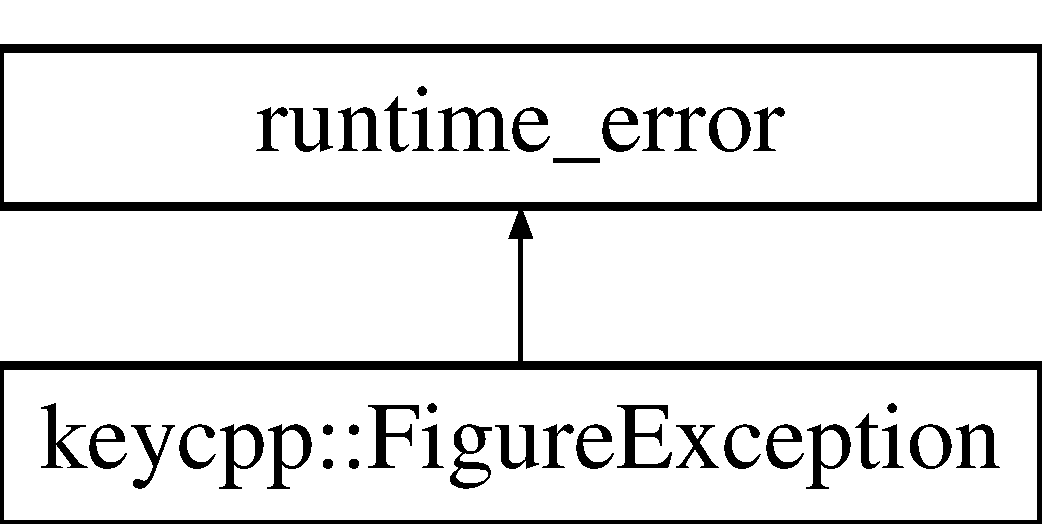
\includegraphics[height=2.000000cm]{classkeycpp_1_1_figure_exception}
\end{center}
\end{figure}
\subsection*{Public Member Functions}
\begin{DoxyCompactItemize}
\item 
\hypertarget{classkeycpp_1_1_figure_exception_aacd7cab583d3eea1ddd185a8fd7b1133}{{\bfseries Figure\-Exception} (const std\-::string \&msg)}\label{classkeycpp_1_1_figure_exception_aacd7cab583d3eea1ddd185a8fd7b1133}

\end{DoxyCompactItemize}


The documentation for this class was generated from the following file\-:\begin{DoxyCompactItemize}
\item 
Figure.\-h\end{DoxyCompactItemize}

\hypertarget{class_gnuplot}{\section{Gnuplot Class Reference}
\label{class_gnuplot}\index{Gnuplot@{Gnuplot}}
}
\subsection*{Public Member Functions}
\begin{DoxyCompactItemize}
\item 
\hypertarget{class_gnuplot_a187eb517b362cf379492fe7f1621ee50}{\hyperlink{class_gnuplot_a187eb517b362cf379492fe7f1621ee50}{Gnuplot} (const std\-::string \&style=\char`\"{}points\char`\"{})}\label{class_gnuplot_a187eb517b362cf379492fe7f1621ee50}

\begin{DoxyCompactList}\small\item\em set a style during construction \end{DoxyCompactList}\item 
\hypertarget{class_gnuplot_a8ceac5808e42665c1dee305ae7ea9070}{\hyperlink{class_gnuplot_a8ceac5808e42665c1dee305ae7ea9070}{Gnuplot} (const std\-::vector$<$ double $>$ \&x, const std\-::string \&title=\char`\"{}\char`\"{}, const std\-::string \&style=\char`\"{}points\char`\"{}, const std\-::string \&labelx=\char`\"{}x\char`\"{}, const std\-::string \&labely=\char`\"{}y\char`\"{})}\label{class_gnuplot_a8ceac5808e42665c1dee305ae7ea9070}

\begin{DoxyCompactList}\small\item\em plot a single std\-::vector at one go \end{DoxyCompactList}\item 
\hypertarget{class_gnuplot_a24327b6116c71acdc195eadf665c67cb}{\hyperlink{class_gnuplot_a24327b6116c71acdc195eadf665c67cb}{Gnuplot} (const std\-::vector$<$ double $>$ \&x, const std\-::vector$<$ double $>$ \&y, const std\-::string \&title=\char`\"{}\char`\"{}, const std\-::string \&style=\char`\"{}points\char`\"{}, const std\-::string \&labelx=\char`\"{}x\char`\"{}, const std\-::string \&labely=\char`\"{}y\char`\"{})}\label{class_gnuplot_a24327b6116c71acdc195eadf665c67cb}

\begin{DoxyCompactList}\small\item\em plot pairs std\-::vector at one go \end{DoxyCompactList}\item 
\hypertarget{class_gnuplot_a14191e89154f2716608f6907975cc012}{\hyperlink{class_gnuplot_a14191e89154f2716608f6907975cc012}{Gnuplot} (const std\-::vector$<$ double $>$ \&x, const std\-::vector$<$ double $>$ \&y, const std\-::vector$<$ double $>$ \&z, const std\-::string \&title=\char`\"{}\char`\"{}, const std\-::string \&style=\char`\"{}points\char`\"{}, const std\-::string \&labelx=\char`\"{}x\char`\"{}, const std\-::string \&labely=\char`\"{}y\char`\"{}, const std\-::string \&labelz=\char`\"{}z\char`\"{})}\label{class_gnuplot_a14191e89154f2716608f6907975cc012}

\begin{DoxyCompactList}\small\item\em plot triples std\-::vector at one go \end{DoxyCompactList}\item 
\hypertarget{class_gnuplot_a78a68f621caa87d1f34324fcd093c7bd}{\hyperlink{class_gnuplot_a78a68f621caa87d1f34324fcd093c7bd}{$\sim$\-Gnuplot} ()}\label{class_gnuplot_a78a68f621caa87d1f34324fcd093c7bd}

\begin{DoxyCompactList}\small\item\em destructor\-: needed to delete temporary files \end{DoxyCompactList}\item 
\hypertarget{class_gnuplot_a07607803ede8dd5416906df0a1924fc5}{\hyperlink{class_gnuplot}{Gnuplot} \& \hyperlink{class_gnuplot_a07607803ede8dd5416906df0a1924fc5}{cmd} (const std\-::string \&cmdstr)}\label{class_gnuplot_a07607803ede8dd5416906df0a1924fc5}

\begin{DoxyCompactList}\small\item\em send a command to gnuplot \end{DoxyCompactList}\item 
\hyperlink{class_gnuplot}{Gnuplot} \& \hyperlink{class_gnuplot_afb69631c7a498077e378a3cbb56f38c8}{operator$<$$<$} (const std\-::string \&cmdstr)
\begin{DoxyCompactList}\small\item\em Sends a command to an active gnuplot session, identical to \hyperlink{class_gnuplot_a07607803ede8dd5416906df0a1924fc5}{cmd()} send a command to gnuplot using the $<$$<$ operator. \end{DoxyCompactList}\item 
\hypertarget{class_gnuplot_a356d2faaa79f08d13fec9718b776b28d}{\hyperlink{class_gnuplot}{Gnuplot} \& \hyperlink{class_gnuplot_a356d2faaa79f08d13fec9718b776b28d}{showonscreen} ()}\label{class_gnuplot_a356d2faaa79f08d13fec9718b776b28d}

\begin{DoxyCompactList}\small\item\em sets terminal type to terminal\-\_\-std \end{DoxyCompactList}\item 
\hypertarget{class_gnuplot_a1ccaa142290490429c6cd623543a914c}{\hyperlink{class_gnuplot}{Gnuplot} \& \hyperlink{class_gnuplot_a1ccaa142290490429c6cd623543a914c}{savetofigure} (const std\-::string filename, const std\-::string terminal=\char`\"{}ps\char`\"{})}\label{class_gnuplot_a1ccaa142290490429c6cd623543a914c}

\begin{DoxyCompactList}\small\item\em Saves a gnuplot to a file named filename. Defaults to saving pdf. \end{DoxyCompactList}\item 
\hyperlink{class_gnuplot}{Gnuplot} \& \hyperlink{class_gnuplot_acfdcda292650775ebed4683e8e1515b5}{set\-\_\-style} (const std\-::string \&stylestr=\char`\"{}points\char`\"{})
\item 
\hyperlink{class_gnuplot}{Gnuplot} \& \hyperlink{class_gnuplot_aa18386919da2ec4c994f1f9c7195d384}{set\-\_\-smooth} (const std\-::string \&stylestr=\char`\"{}csplines\char`\"{})
\item 
\hyperlink{class_gnuplot}{Gnuplot} \& \hyperlink{class_gnuplot_ad9dfbccd66dece1dbe5803605c6ab08c}{unset\-\_\-smooth} ()
\begin{DoxyCompactList}\small\item\em unset smooth attention\-: smooth is not set by default \end{DoxyCompactList}\item 
\hypertarget{class_gnuplot_a95ec1636a871447dfe99463b769339c7}{\hyperlink{class_gnuplot}{Gnuplot} \& \hyperlink{class_gnuplot_a95ec1636a871447dfe99463b769339c7}{set\-\_\-pointsize} (const double pointsize=1.\-0)}\label{class_gnuplot_a95ec1636a871447dfe99463b769339c7}

\begin{DoxyCompactList}\small\item\em scales the size of the points used in plots \end{DoxyCompactList}\item 
\hypertarget{class_gnuplot_a5416c8e81f1b9945b9631fa85a8d4f47}{\hyperlink{class_gnuplot}{Gnuplot} \& \hyperlink{class_gnuplot_a5416c8e81f1b9945b9631fa85a8d4f47}{set\-\_\-grid} ()}\label{class_gnuplot_a5416c8e81f1b9945b9631fa85a8d4f47}

\begin{DoxyCompactList}\small\item\em turns grid on/off \end{DoxyCompactList}\item 
\hypertarget{class_gnuplot_a53183e1487bc6977f0d46bf75d19b4d3}{\hyperlink{class_gnuplot}{Gnuplot} \& \hyperlink{class_gnuplot_a53183e1487bc6977f0d46bf75d19b4d3}{unset\-\_\-grid} ()}\label{class_gnuplot_a53183e1487bc6977f0d46bf75d19b4d3}

\begin{DoxyCompactList}\small\item\em grid is not set by default \end{DoxyCompactList}\item 
\hyperlink{class_gnuplot}{Gnuplot} \& \hyperlink{class_gnuplot_a67efc4d4dc46b6100d14ba2f7366ef11}{set\-\_\-multiplot} ()
\item 
\hyperlink{class_gnuplot}{Gnuplot} \& \hyperlink{class_gnuplot_aad76cdec16cfb5fdf82f45ed2786f4d8}{unset\-\_\-multiplot} ()
\item 
\hypertarget{class_gnuplot_a671cbe7b18a267ea59f532c83a0035f6}{\hyperlink{class_gnuplot}{Gnuplot} \& \hyperlink{class_gnuplot_a671cbe7b18a267ea59f532c83a0035f6}{set\-\_\-samples} (const int samples=100)}\label{class_gnuplot_a671cbe7b18a267ea59f532c83a0035f6}

\begin{DoxyCompactList}\small\item\em set sampling rate of functions, or for interpolating data \end{DoxyCompactList}\item 
\hypertarget{class_gnuplot_ab810fa4c02fb49ae197786c305b78702}{\hyperlink{class_gnuplot}{Gnuplot} \& \hyperlink{class_gnuplot_ab810fa4c02fb49ae197786c305b78702}{set\-\_\-isosamples} (const int isolines=10)}\label{class_gnuplot_ab810fa4c02fb49ae197786c305b78702}

\begin{DoxyCompactList}\small\item\em set isoline density (grid) for plotting functions as surfaces (for 3d plots) \end{DoxyCompactList}\item 
\hyperlink{class_gnuplot}{Gnuplot} \& \hyperlink{class_gnuplot_a891f9800705eddc3f73886f265c009b8}{set\-\_\-hidden3d} ()
\item 
\hyperlink{class_gnuplot}{Gnuplot} \& \hyperlink{class_gnuplot_ab8688182047f746090e1e5f2a8c11c9e}{unset\-\_\-hidden3d} ()
\item 
\hyperlink{class_gnuplot}{Gnuplot} \& \hyperlink{class_gnuplot_af845efc728a90d7e10de764eff0b2423}{set\-\_\-contour} (const std\-::string \&position=\char`\"{}base\char`\"{})
\item 
\hyperlink{class_gnuplot}{Gnuplot} \& \hyperlink{class_gnuplot_a0b8522cb81e46dd4f5a22b7b48f977b1}{unset\-\_\-contour} ()
\item 
\hyperlink{class_gnuplot}{Gnuplot} \& \hyperlink{class_gnuplot_a9825bd26500e30ca88404c4807e6607a}{set\-\_\-surface} ()
\item 
\hyperlink{class_gnuplot}{Gnuplot} \& \hyperlink{class_gnuplot_a4ebddacbec61aa3e7bc4b89f508ad621}{unset\-\_\-surface} ()
\item 
\hyperlink{class_gnuplot}{Gnuplot} \& \hyperlink{class_gnuplot_ad64a717dac18167f656c4f09239973f8}{set\-\_\-legend} (const std\-::string \&position=\char`\"{}default\char`\"{})
\item 
\hyperlink{class_gnuplot}{Gnuplot} \& \hyperlink{class_gnuplot_ace901a18ab1a459213afd3ee0233b5ce}{unset\-\_\-legend} ()
\begin{DoxyCompactList}\small\item\em Switches legend off attention\-:legend is set by default. \end{DoxyCompactList}\item 
\hyperlink{class_gnuplot}{Gnuplot} \& \hyperlink{class_gnuplot_a4f93bac0e69dd83806652ca7226c6b3b}{set\-\_\-title} (const std\-::string \&title=\char`\"{}\char`\"{})
\begin{DoxyCompactList}\small\item\em sets and clears the title of a gnuplot session \end{DoxyCompactList}\item 
\hyperlink{class_gnuplot}{Gnuplot} \& \hyperlink{class_gnuplot_aca0aeb1dc0ac8d7e68ba6a15a977be28}{unset\-\_\-title} ()
\begin{DoxyCompactList}\small\item\em Clears the title of a gnuplot session The title is not set by default. \end{DoxyCompactList}\item 
\hypertarget{class_gnuplot_afcb311938827f8718f19ed52d66bad7c}{\hyperlink{class_gnuplot}{Gnuplot} \& \hyperlink{class_gnuplot_afcb311938827f8718f19ed52d66bad7c}{set\-\_\-ylabel} (const std\-::string \&label=\char`\"{}x\char`\"{})}\label{class_gnuplot_afcb311938827f8718f19ed52d66bad7c}

\begin{DoxyCompactList}\small\item\em set x axis label \end{DoxyCompactList}\item 
\hypertarget{class_gnuplot_aa93589a95aeab869ba731e2583843ae4}{\hyperlink{class_gnuplot}{Gnuplot} \& \hyperlink{class_gnuplot_aa93589a95aeab869ba731e2583843ae4}{set\-\_\-xlabel} (const std\-::string \&label=\char`\"{}y\char`\"{})}\label{class_gnuplot_aa93589a95aeab869ba731e2583843ae4}

\begin{DoxyCompactList}\small\item\em set y axis label \end{DoxyCompactList}\item 
\hypertarget{class_gnuplot_ab3206e715d20f05cc0dd1eec89ce8b07}{\hyperlink{class_gnuplot}{Gnuplot} \& \hyperlink{class_gnuplot_ab3206e715d20f05cc0dd1eec89ce8b07}{set\-\_\-zlabel} (const std\-::string \&label=\char`\"{}z\char`\"{})}\label{class_gnuplot_ab3206e715d20f05cc0dd1eec89ce8b07}

\begin{DoxyCompactList}\small\item\em set z axis label \end{DoxyCompactList}\item 
\hypertarget{class_gnuplot_a4b8d96018f2d2d4e2922d4df153d6a84}{\hyperlink{class_gnuplot}{Gnuplot} \& \hyperlink{class_gnuplot_a4b8d96018f2d2d4e2922d4df153d6a84}{set\-\_\-xrange} (const double i\-From, const double i\-To)}\label{class_gnuplot_a4b8d96018f2d2d4e2922d4df153d6a84}

\begin{DoxyCompactList}\small\item\em set axis -\/ ranges \end{DoxyCompactList}\item 
\hypertarget{class_gnuplot_a461271b7bfd4f84bdfc0055457226f28}{\hyperlink{class_gnuplot}{Gnuplot} \& \hyperlink{class_gnuplot_a461271b7bfd4f84bdfc0055457226f28}{set\-\_\-yrange} (const double i\-From, const double i\-To)}\label{class_gnuplot_a461271b7bfd4f84bdfc0055457226f28}

\begin{DoxyCompactList}\small\item\em set y-\/axis -\/ ranges \end{DoxyCompactList}\item 
\hypertarget{class_gnuplot_a7273f6a48024117b4d234d0251106e78}{\hyperlink{class_gnuplot}{Gnuplot} \& \hyperlink{class_gnuplot_a7273f6a48024117b4d234d0251106e78}{set\-\_\-zrange} (const double i\-From, const double i\-To)}\label{class_gnuplot_a7273f6a48024117b4d234d0251106e78}

\begin{DoxyCompactList}\small\item\em set z-\/axis -\/ ranges \end{DoxyCompactList}\item 
\hyperlink{class_gnuplot}{Gnuplot} \& \hyperlink{class_gnuplot_a11a62a04c203f01607c3c21a727e318d}{set\-\_\-xautoscale} ()
\item 
\hyperlink{class_gnuplot}{Gnuplot} \& \hyperlink{class_gnuplot_a5b9e1a4e68f94d418a8e9194f168b448}{set\-\_\-yautoscale} ()
\item 
\hyperlink{class_gnuplot}{Gnuplot} \& \hyperlink{class_gnuplot_aef3e84e793836158e1ddd773d1465c37}{set\-\_\-zautoscale} ()
\item 
\hypertarget{class_gnuplot_aff546fad227d93babeb5d2cc9f047b89}{\hyperlink{class_gnuplot}{Gnuplot} \& \hyperlink{class_gnuplot_aff546fad227d93babeb5d2cc9f047b89}{set\-\_\-xlogscale} (const double base=10)}\label{class_gnuplot_aff546fad227d93babeb5d2cc9f047b89}

\begin{DoxyCompactList}\small\item\em turns on/off log scaling for the specified xaxis (logscale is not set by default) \end{DoxyCompactList}\item 
\hypertarget{class_gnuplot_a201a802d2f27fece0d39809c4eb3bce0}{\hyperlink{class_gnuplot}{Gnuplot} \& \hyperlink{class_gnuplot_a201a802d2f27fece0d39809c4eb3bce0}{set\-\_\-ylogscale} (const double base=10)}\label{class_gnuplot_a201a802d2f27fece0d39809c4eb3bce0}

\begin{DoxyCompactList}\small\item\em turns on/off log scaling for the specified yaxis (logscale is not set by default) \end{DoxyCompactList}\item 
\hypertarget{class_gnuplot_a1da3838163b0dbde8809b55c5b5c56b1}{\hyperlink{class_gnuplot}{Gnuplot} \& \hyperlink{class_gnuplot_a1da3838163b0dbde8809b55c5b5c56b1}{set\-\_\-zlogscale} (const double base=10)}\label{class_gnuplot_a1da3838163b0dbde8809b55c5b5c56b1}

\begin{DoxyCompactList}\small\item\em turns on/off log scaling for the specified zaxis (logscale is not set by default) \end{DoxyCompactList}\item 
\hyperlink{class_gnuplot}{Gnuplot} \& \hyperlink{class_gnuplot_a7b178184260f1498cd0c11a197ea0ac2}{unset\-\_\-xlogscale} ()
\item 
\hyperlink{class_gnuplot}{Gnuplot} \& \hyperlink{class_gnuplot_a9217543dd49c4802b1194d42c5e10b6d}{unset\-\_\-ylogscale} ()
\item 
\hyperlink{class_gnuplot}{Gnuplot} \& \hyperlink{class_gnuplot_afa67f022ca344593b054d7f2e3406c7e}{unset\-\_\-zlogscale} ()
\item 
\hypertarget{class_gnuplot_a2228f5ab4cce2da463fc90383076a598}{\hyperlink{class_gnuplot}{Gnuplot} \& \hyperlink{class_gnuplot_a2228f5ab4cce2da463fc90383076a598}{set\-\_\-cbrange} (const double i\-From, const double i\-To)}\label{class_gnuplot_a2228f5ab4cce2da463fc90383076a598}

\begin{DoxyCompactList}\small\item\em set palette range (autoscale by default) \end{DoxyCompactList}\item 
\hyperlink{class_gnuplot}{Gnuplot} \& \hyperlink{class_gnuplot_a4fc34218cdfdd27a65b92eea1f1f9e84}{plotfile\-\_\-x} (const std\-::string \&filename, const unsigned int column=1, const std\-::string \&title=\char`\"{}\char`\"{})
\item 
{\footnotesize template$<$typename X $>$ }\\\hyperlink{class_gnuplot}{Gnuplot} \& \hyperlink{class_gnuplot_a80f3b2baae2bceff78ad005d9c3ec3fb}{plot\-\_\-x} (const X \&x, const std\-::string \&title=\char`\"{}\char`\"{})
\begin{DoxyCompactList}\small\item\em from std\-::vector \end{DoxyCompactList}\item 
\hyperlink{class_gnuplot}{Gnuplot} \& \hyperlink{class_gnuplot_a10e1fc7344bd726faa2d70cd5ced5e5e}{plotfile\-\_\-xy} (const std\-::string \&filename, const unsigned int column\-\_\-x=1, const unsigned int column\-\_\-y=2, const std\-::string \&title=\char`\"{}\char`\"{})
\item 
{\footnotesize template$<$typename X , typename Y $>$ }\\\hyperlink{class_gnuplot}{Gnuplot} \& \hyperlink{class_gnuplot_a0514a7391de6b42e79732ce746c310f7}{plot\-\_\-xy} (const X \&x, const Y \&y, const std\-::string \&title=\char`\"{}\char`\"{})
\begin{DoxyCompactList}\small\item\em from data \end{DoxyCompactList}\item 
\hyperlink{class_gnuplot}{Gnuplot} \& \hyperlink{class_gnuplot_a26cbba36864ad7f1f6683b11558e3b49}{plotfile\-\_\-xyy} (const std\-::string \&filename, const unsigned int column\-\_\-x=1, const unsigned int column\-\_\-y1=2, const unsigned int column\-\_\-y2=3, const std\-::string \&title1=\char`\"{}\char`\"{}, const std\-::string \&title2=\char`\"{}\char`\"{})
\item 
\hypertarget{class_gnuplot_ac0c275ff75d700fc8e9f55d15dea1ea3}{{\footnotesize template$<$typename X , typename Y $>$ }\\\hyperlink{class_gnuplot}{Gnuplot} \& \hyperlink{class_gnuplot_ac0c275ff75d700fc8e9f55d15dea1ea3}{plot\-\_\-xyxy} (const X \&x1, const Y \&y1, const X \&x2, const Y \&y2, const std\-::string \&title1, const std\-::string \&title2, const std\-::string \&style1=\char`\"{}\char`\"{}, const std\-::string \&style2=\char`\"{}\char`\"{})}\label{class_gnuplot_ac0c275ff75d700fc8e9f55d15dea1ea3}

\begin{DoxyCompactList}\small\item\em Plots a 2d graph from a list of doubles\-: x y. \end{DoxyCompactList}\item 
\hyperlink{class_gnuplot}{Gnuplot} \& \hyperlink{class_gnuplot_a4410bb4c65aaf43b0ad5e510da15e20f}{plotfile\-\_\-xyxy} (const std\-::string \&filename1, const std\-::string \&filename2, const unsigned int column\-\_\-x1=1, const unsigned int column\-\_\-y1=2, const unsigned int column\-\_\-x2=1, const unsigned int column\-\_\-y2=2, const std\-::string \&title1=\char`\"{}\char`\"{}, const std\-::string \&title2=\char`\"{}\char`\"{}, const std\-::string \&style1=\char`\"{}\char`\"{}, const std\-::string \&style2=\char`\"{}\char`\"{})
\item 
{\footnotesize template$<$typename X , typename Y $>$ }\\\hyperlink{class_gnuplot}{Gnuplot} \& \hyperlink{class_gnuplot_a9ac40f453f4951f5df8212612b2b5cfd}{plot\-\_\-xyy} (const X \&x, const Y \&y1, const Y \&y2, const std\-::string \&title1=\char`\"{}\char`\"{}, const std\-::string \&title2=\char`\"{}\char`\"{})
\begin{DoxyCompactList}\small\item\em from data \end{DoxyCompactList}\item 
\hyperlink{class_gnuplot}{Gnuplot} \& \hyperlink{class_gnuplot_ac2dcfa52e5758e6472c1c161f52803af}{plotfile\-\_\-xxy} (const std\-::string \&filename, const unsigned int column\-\_\-x1=1, const unsigned int column\-\_\-x2=2, const unsigned int column\-\_\-y=3, const std\-::string \&title1=\char`\"{}\char`\"{}, const std\-::string \&title2=\char`\"{}\char`\"{})
\item 
{\footnotesize template$<$typename X , typename Y $>$ }\\\hyperlink{class_gnuplot}{Gnuplot} \& \hyperlink{class_gnuplot_a5be0d83b9fe1c9123ac4868746eda15d}{plot\-\_\-xxy} (const X \&x1, const X \&x2, const Y \&y, const std\-::string \&title1=\char`\"{}\char`\"{}, const std\-::string \&title2=\char`\"{}\char`\"{})
\begin{DoxyCompactList}\small\item\em from data \end{DoxyCompactList}\item 
\hyperlink{class_gnuplot}{Gnuplot} \& \hyperlink{class_gnuplot_a6446b66df4b42691a8cd4b9c2b04f250}{plotfile\-\_\-xxxxy} (const std\-::string \&filename, const unsigned int column\-\_\-x1=1, const unsigned int column\-\_\-x2=2, const unsigned int column\-\_\-x3=3, const unsigned int column\-\_\-x4=4, const unsigned int column\-\_\-y=5, const std\-::string \&title1=\char`\"{}\char`\"{}, const std\-::string \&title2=\char`\"{}\char`\"{}, const std\-::string \&title3=\char`\"{}\char`\"{}, const std\-::string \&title4=\char`\"{}\char`\"{})
\item 
{\footnotesize template$<$typename X , typename Y $>$ }\\\hyperlink{class_gnuplot}{Gnuplot} \& \hyperlink{class_gnuplot_aa4736bcf899c4b2454117f9377a707e3}{plot\-\_\-xxxxy} (const X \&x1, const X \&x2, const X \&x3, const X \&x4, const Y \&y, const std\-::string \&title1=\char`\"{}\char`\"{}, const std\-::string \&title2=\char`\"{}\char`\"{}, const std\-::string \&title3=\char`\"{}\char`\"{}, const std\-::string \&title4=\char`\"{}\char`\"{})
\begin{DoxyCompactList}\small\item\em from data \end{DoxyCompactList}\item 
\hyperlink{class_gnuplot}{Gnuplot} \& \hyperlink{class_gnuplot_afe9d44ba12f617188111ab915010f3ab}{plotfile\-\_\-xy\-\_\-err} (const std\-::string \&filename, const unsigned int column\-\_\-x=1, const unsigned int column\-\_\-y=2, const unsigned int column\-\_\-dy=3, const std\-::string \&title=\char`\"{}\char`\"{})
\item 
{\footnotesize template$<$typename X , typename Y , typename E $>$ }\\\hyperlink{class_gnuplot}{Gnuplot} \& \hyperlink{class_gnuplot_a3c5d382eba33f92b26ba85f201bc7dea}{plot\-\_\-xy\-\_\-err} (const X \&x, const Y \&y, const E \&dy, const std\-::string \&title=\char`\"{}\char`\"{})
\begin{DoxyCompactList}\small\item\em from data \end{DoxyCompactList}\item 
\hyperlink{class_gnuplot}{Gnuplot} \& \hyperlink{class_gnuplot_a9dbde2a91eb816481657f3a22c9b0046}{plotfile\-\_\-xyz} (const std\-::string \&filename, const unsigned int column\-\_\-x=1, const unsigned int column\-\_\-y=2, const unsigned int column\-\_\-z=3, const std\-::string \&title=\char`\"{}\char`\"{})
\item 
\hypertarget{class_gnuplot_af89cb366fa7d09ffc1c351516ae54df5}{{\footnotesize template$<$typename X , typename Y , typename Z $>$ }\\\hyperlink{class_gnuplot}{Gnuplot} \& \hyperlink{class_gnuplot_af89cb366fa7d09ffc1c351516ae54df5}{plot\-\_\-xyz} (const X \&x, const Y \&y, const Z \&z, const std\-::string \&title=\char`\"{}\char`\"{})}\label{class_gnuplot_af89cb366fa7d09ffc1c351516ae54df5}

\begin{DoxyCompactList}\small\item\em from std\-::vector \end{DoxyCompactList}\item 
\hypertarget{class_gnuplot_a51ea5105eb87285820bb93910f8d346c}{\hyperlink{class_gnuplot}{Gnuplot} \& \hyperlink{class_gnuplot_a51ea5105eb87285820bb93910f8d346c}{plot\-\_\-slope} (const double a, const double b, const std\-::string \&title=\char`\"{}\char`\"{})}\label{class_gnuplot_a51ea5105eb87285820bb93910f8d346c}

\begin{DoxyCompactList}\small\item\em plot an equation of the form\-: y = ax + b, you supply a and b \end{DoxyCompactList}\item 
\hyperlink{class_gnuplot}{Gnuplot} \& \hyperlink{class_gnuplot_a42dfb8c9d4636745c7be277ed818e849}{plot\-\_\-equation} (const std\-::string \&equation, const std\-::string \&title=\char`\"{}\char`\"{})
\item 
\hyperlink{class_gnuplot}{Gnuplot} \& \hyperlink{class_gnuplot_a79aed3a6927f7d1d3497cba441e8a943}{plot\-\_\-equation3d} (const std\-::string \&equation, const std\-::string \&title=\char`\"{}\char`\"{})
\item 
\hyperlink{class_gnuplot}{Gnuplot} \& \hyperlink{class_gnuplot_aae22c0470a6fbbc1f5e84dec8d023381}{plot\-\_\-image} (const unsigned char $\ast$uc\-Pic\-Buf, const unsigned int i\-Width, const unsigned int i\-Height, const std\-::string \&title=\char`\"{}\char`\"{})
\begin{DoxyCompactList}\small\item\em plot image \end{DoxyCompactList}\item 
\hyperlink{class_gnuplot}{Gnuplot} \& \hyperlink{class_gnuplot_a34c1b3e877d246a841a29f857a29f502}{replot} (void)
\begin{DoxyCompactList}\small\item\em replot repeats the last plot or splot command. this can be useful for viewing a plot with different set options, or when generating the same plot for several devices (showonscreen, \end{DoxyCompactList}\item 
\hypertarget{class_gnuplot_a6797761712d3c311e3685bcccba65dd4}{\hyperlink{class_gnuplot}{Gnuplot} \& \hyperlink{class_gnuplot_a6797761712d3c311e3685bcccba65dd4}{reset\-\_\-plot} ()}\label{class_gnuplot_a6797761712d3c311e3685bcccba65dd4}

\begin{DoxyCompactList}\small\item\em resets a gnuplot session (next plot will erase previous ones) \end{DoxyCompactList}\item 
\hypertarget{class_gnuplot_a9aedfe8371083a1a3ac2b9493810049c}{\hyperlink{class_gnuplot}{Gnuplot} \& \hyperlink{class_gnuplot_a9aedfe8371083a1a3ac2b9493810049c}{reset\-\_\-all} ()}\label{class_gnuplot_a9aedfe8371083a1a3ac2b9493810049c}

\begin{DoxyCompactList}\small\item\em resets a gnuplot session and sets all variables to default \end{DoxyCompactList}\item 
\hypertarget{class_gnuplot_a2e449552587b0055f40f4ee079d62a8d}{void \hyperlink{class_gnuplot_a2e449552587b0055f40f4ee079d62a8d}{remove\-\_\-tmpfiles} ()}\label{class_gnuplot_a2e449552587b0055f40f4ee079d62a8d}

\begin{DoxyCompactList}\small\item\em deletes temporary files \end{DoxyCompactList}\item 
bool \hyperlink{class_gnuplot_a3135ffebb308b50c4f3178a62b23ab03}{is\-\_\-valid} ()
\begin{DoxyCompactList}\small\item\em Is the gnuplot session valid ?? \end{DoxyCompactList}\end{DoxyCompactItemize}
\subsection*{Static Public Member Functions}
\begin{DoxyCompactItemize}
\item 
static bool \hyperlink{class_gnuplot_a67cae885c26ced821e335d98986f1967}{set\-\_\-\-G\-N\-U\-Plot\-Path} (const std\-::string \&path)
\begin{DoxyCompactList}\small\item\em optional function\-: set \hyperlink{class_gnuplot}{Gnuplot} path manual attention\-: for windows\-: path with slash '/' not backslash '\textbackslash{}' \end{DoxyCompactList}\item 
static void \hyperlink{class_gnuplot_a21feba7a3916708b742c3dc25850ab2f}{set\-\_\-terminal\-\_\-std} (const std\-::string \&type)
\end{DoxyCompactItemize}


\subsection{Member Function Documentation}
\hypertarget{class_gnuplot_a3135ffebb308b50c4f3178a62b23ab03}{\index{Gnuplot@{Gnuplot}!is\-\_\-valid@{is\-\_\-valid}}
\index{is\-\_\-valid@{is\-\_\-valid}!Gnuplot@{Gnuplot}}
\subsubsection[{is\-\_\-valid}]{\setlength{\rightskip}{0pt plus 5cm}bool Gnuplot\-::is\-\_\-valid (
\begin{DoxyParamCaption}
{}
\end{DoxyParamCaption}
)\hspace{0.3cm}{\ttfamily [inline]}}}\label{class_gnuplot_a3135ffebb308b50c4f3178a62b23ab03}

\begin{DoxyParams}{Parameters}
{\em \&mdash;} & \\
\hline
\end{DoxyParams}
\begin{DoxyReturn}{Returns}
true if valid, false if not 
\end{DoxyReturn}
\hypertarget{class_gnuplot_afb69631c7a498077e378a3cbb56f38c8}{\index{Gnuplot@{Gnuplot}!operator$<$$<$@{operator$<$$<$}}
\index{operator$<$$<$@{operator$<$$<$}!Gnuplot@{Gnuplot}}
\subsubsection[{operator$<$$<$}]{\setlength{\rightskip}{0pt plus 5cm}{\bf Gnuplot}\& Gnuplot\-::operator$<$$<$ (
\begin{DoxyParamCaption}
\item[{const std\-::string \&}]{cmdstr}
\end{DoxyParamCaption}
)\hspace{0.3cm}{\ttfamily [inline]}}}\label{class_gnuplot_afb69631c7a498077e378a3cbb56f38c8}

\begin{DoxyParams}{Parameters}
{\em cmdstr} & --$>$ the command string\\
\hline
\end{DoxyParams}
\begin{DoxyReturn}{Returns}
$<$-- a reference to the gnuplot object 
\end{DoxyReturn}
\hypertarget{class_gnuplot_a42dfb8c9d4636745c7be277ed818e849}{\index{Gnuplot@{Gnuplot}!plot\-\_\-equation@{plot\-\_\-equation}}
\index{plot\-\_\-equation@{plot\-\_\-equation}!Gnuplot@{Gnuplot}}
\subsubsection[{plot\-\_\-equation}]{\setlength{\rightskip}{0pt plus 5cm}{\bf Gnuplot} \& Gnuplot\-::plot\-\_\-equation (
\begin{DoxyParamCaption}
\item[{const std\-::string \&}]{equation, }
\item[{const std\-::string \&}]{title = {\ttfamily \char`\"{}\char`\"{}}}
\end{DoxyParamCaption}
)}}\label{class_gnuplot_a42dfb8c9d4636745c7be277ed818e849}
plot an equation supplied as a std\-::string y=f(x), write only the function f(x) not y the independent variable has to be x binary operators\-: $\ast$$\ast$ exponentiation, $\ast$ multiply, / divide, + add, -\/ substract, \% modulo unary operators\-: -\/ minus, ! factorial elementary functions\-: rand(x), abs(x), sgn(x), ceil(x), floor(x), int(x), imag(x), real(x), arg(x), sqrt(x), exp(x), log(x), log10(x), sin(x), cos(x), tan(x), asin(x), acos(x), atan(x), atan2(y,x), sinh(x), cosh(x), tanh(x), asinh(x), acosh(x), atanh(x) special functions\-: erf(x), erfc(x), inverf(x), gamma(x), igamma(a,x), lgamma(x), ibeta(p,q,x), besj0(x), besj1(x), besy0(x), besy1(x), lambertw(x) statistical fuctions\-: norm(x), invnorm(x) \hypertarget{class_gnuplot_a79aed3a6927f7d1d3497cba441e8a943}{\index{Gnuplot@{Gnuplot}!plot\-\_\-equation3d@{plot\-\_\-equation3d}}
\index{plot\-\_\-equation3d@{plot\-\_\-equation3d}!Gnuplot@{Gnuplot}}
\subsubsection[{plot\-\_\-equation3d}]{\setlength{\rightskip}{0pt plus 5cm}{\bf Gnuplot} \& Gnuplot\-::plot\-\_\-equation3d (
\begin{DoxyParamCaption}
\item[{const std\-::string \&}]{equation, }
\item[{const std\-::string \&}]{title = {\ttfamily \char`\"{}\char`\"{}}}
\end{DoxyParamCaption}
)}}\label{class_gnuplot_a79aed3a6927f7d1d3497cba441e8a943}
plot an equation supplied as a std\-::string z=f(x,y), write only the function f(x,y) not z the independent variables have to be x and y \hypertarget{class_gnuplot_aae22c0470a6fbbc1f5e84dec8d023381}{\index{Gnuplot@{Gnuplot}!plot\-\_\-image@{plot\-\_\-image}}
\index{plot\-\_\-image@{plot\-\_\-image}!Gnuplot@{Gnuplot}}
\subsubsection[{plot\-\_\-image}]{\setlength{\rightskip}{0pt plus 5cm}{\bf Gnuplot} \& Gnuplot\-::plot\-\_\-image (
\begin{DoxyParamCaption}
\item[{const unsigned char $\ast$}]{uc\-Pic\-Buf, }
\item[{const unsigned int}]{i\-Width, }
\item[{const unsigned int}]{i\-Height, }
\item[{const std\-::string \&}]{title = {\ttfamily \char`\"{}\char`\"{}}}
\end{DoxyParamCaption}
)}}\label{class_gnuplot_aae22c0470a6fbbc1f5e84dec8d023381}

\begin{DoxyItemize}
\item note that this function is not valid for versions of G\-N\-U\-Plot below 4.\-2 
\end{DoxyItemize}\hypertarget{class_gnuplot_a80f3b2baae2bceff78ad005d9c3ec3fb}{\index{Gnuplot@{Gnuplot}!plot\-\_\-x@{plot\-\_\-x}}
\index{plot\-\_\-x@{plot\-\_\-x}!Gnuplot@{Gnuplot}}
\subsubsection[{plot\-\_\-x}]{\setlength{\rightskip}{0pt plus 5cm}template$<$typename X $>$ {\bf Gnuplot} \& Gnuplot\-::plot\-\_\-x (
\begin{DoxyParamCaption}
\item[{const X \&}]{x, }
\item[{const std\-::string \&}]{title = {\ttfamily \char`\"{}\char`\"{}}}
\end{DoxyParamCaption}
)}}\label{class_gnuplot_a80f3b2baae2bceff78ad005d9c3ec3fb}
Plots a 2d graph from a list of doubles\-: x. \hypertarget{class_gnuplot_aa4736bcf899c4b2454117f9377a707e3}{\index{Gnuplot@{Gnuplot}!plot\-\_\-xxxxy@{plot\-\_\-xxxxy}}
\index{plot\-\_\-xxxxy@{plot\-\_\-xxxxy}!Gnuplot@{Gnuplot}}
\subsubsection[{plot\-\_\-xxxxy}]{\setlength{\rightskip}{0pt plus 5cm}template$<$typename X , typename Y $>$ {\bf Gnuplot} \& Gnuplot\-::plot\-\_\-xxxxy (
\begin{DoxyParamCaption}
\item[{const X \&}]{x1, }
\item[{const X \&}]{x2, }
\item[{const X \&}]{x3, }
\item[{const X \&}]{x4, }
\item[{const Y \&}]{y, }
\item[{const std\-::string \&}]{title1 = {\ttfamily \char`\"{}\char`\"{}}, }
\item[{const std\-::string \&}]{title2 = {\ttfamily \char`\"{}\char`\"{}}, }
\item[{const std\-::string \&}]{title3 = {\ttfamily \char`\"{}\char`\"{}}, }
\item[{const std\-::string \&}]{title4 = {\ttfamily \char`\"{}\char`\"{}}}
\end{DoxyParamCaption}
)}}\label{class_gnuplot_aa4736bcf899c4b2454117f9377a707e3}
Plots a 2d graph from a list of doubles\-: x y. \hypertarget{class_gnuplot_a5be0d83b9fe1c9123ac4868746eda15d}{\index{Gnuplot@{Gnuplot}!plot\-\_\-xxy@{plot\-\_\-xxy}}
\index{plot\-\_\-xxy@{plot\-\_\-xxy}!Gnuplot@{Gnuplot}}
\subsubsection[{plot\-\_\-xxy}]{\setlength{\rightskip}{0pt plus 5cm}template$<$typename X , typename Y $>$ {\bf Gnuplot} \& Gnuplot\-::plot\-\_\-xxy (
\begin{DoxyParamCaption}
\item[{const X \&}]{x1, }
\item[{const X \&}]{x2, }
\item[{const Y \&}]{y, }
\item[{const std\-::string \&}]{title1 = {\ttfamily \char`\"{}\char`\"{}}, }
\item[{const std\-::string \&}]{title2 = {\ttfamily \char`\"{}\char`\"{}}}
\end{DoxyParamCaption}
)}}\label{class_gnuplot_a5be0d83b9fe1c9123ac4868746eda15d}
Plots a 2d graph from a list of doubles\-: x y. \hypertarget{class_gnuplot_a0514a7391de6b42e79732ce746c310f7}{\index{Gnuplot@{Gnuplot}!plot\-\_\-xy@{plot\-\_\-xy}}
\index{plot\-\_\-xy@{plot\-\_\-xy}!Gnuplot@{Gnuplot}}
\subsubsection[{plot\-\_\-xy}]{\setlength{\rightskip}{0pt plus 5cm}template$<$typename X , typename Y $>$ {\bf Gnuplot} \& Gnuplot\-::plot\-\_\-xy (
\begin{DoxyParamCaption}
\item[{const X \&}]{x, }
\item[{const Y \&}]{y, }
\item[{const std\-::string \&}]{title = {\ttfamily \char`\"{}\char`\"{}}}
\end{DoxyParamCaption}
)}}\label{class_gnuplot_a0514a7391de6b42e79732ce746c310f7}
Plots a 2d graph from a list of doubles\-: x y. \hypertarget{class_gnuplot_a3c5d382eba33f92b26ba85f201bc7dea}{\index{Gnuplot@{Gnuplot}!plot\-\_\-xy\-\_\-err@{plot\-\_\-xy\-\_\-err}}
\index{plot\-\_\-xy\-\_\-err@{plot\-\_\-xy\-\_\-err}!Gnuplot@{Gnuplot}}
\subsubsection[{plot\-\_\-xy\-\_\-err}]{\setlength{\rightskip}{0pt plus 5cm}template$<$typename X , typename Y , typename E $>$ {\bf Gnuplot} \& Gnuplot\-::plot\-\_\-xy\-\_\-err (
\begin{DoxyParamCaption}
\item[{const X \&}]{x, }
\item[{const Y \&}]{y, }
\item[{const E \&}]{dy, }
\item[{const std\-::string \&}]{title = {\ttfamily \char`\"{}\char`\"{}}}
\end{DoxyParamCaption}
)}}\label{class_gnuplot_a3c5d382eba33f92b26ba85f201bc7dea}




plot x,y pairs with dy errorbars \hypertarget{class_gnuplot_a9ac40f453f4951f5df8212612b2b5cfd}{\index{Gnuplot@{Gnuplot}!plot\-\_\-xyy@{plot\-\_\-xyy}}
\index{plot\-\_\-xyy@{plot\-\_\-xyy}!Gnuplot@{Gnuplot}}
\subsubsection[{plot\-\_\-xyy}]{\setlength{\rightskip}{0pt plus 5cm}template$<$typename X , typename Y $>$ {\bf Gnuplot} \& Gnuplot\-::plot\-\_\-xyy (
\begin{DoxyParamCaption}
\item[{const X \&}]{x, }
\item[{const Y \&}]{y1, }
\item[{const Y \&}]{y2, }
\item[{const std\-::string \&}]{title1 = {\ttfamily \char`\"{}\char`\"{}}, }
\item[{const std\-::string \&}]{title2 = {\ttfamily \char`\"{}\char`\"{}}}
\end{DoxyParamCaption}
)}}\label{class_gnuplot_a9ac40f453f4951f5df8212612b2b5cfd}
Plots a 2d graph from a list of doubles\-: x y. \hypertarget{class_gnuplot_a4fc34218cdfdd27a65b92eea1f1f9e84}{\index{Gnuplot@{Gnuplot}!plotfile\-\_\-x@{plotfile\-\_\-x}}
\index{plotfile\-\_\-x@{plotfile\-\_\-x}!Gnuplot@{Gnuplot}}
\subsubsection[{plotfile\-\_\-x}]{\setlength{\rightskip}{0pt plus 5cm}{\bf Gnuplot} \& Gnuplot\-::plotfile\-\_\-x (
\begin{DoxyParamCaption}
\item[{const std\-::string \&}]{filename, }
\item[{const unsigned int}]{column = {\ttfamily 1}, }
\item[{const std\-::string \&}]{title = {\ttfamily \char`\"{}\char`\"{}}}
\end{DoxyParamCaption}
)}}\label{class_gnuplot_a4fc34218cdfdd27a65b92eea1f1f9e84}
plot a single std\-::vector\-: x from file \hypertarget{class_gnuplot_a6446b66df4b42691a8cd4b9c2b04f250}{\index{Gnuplot@{Gnuplot}!plotfile\-\_\-xxxxy@{plotfile\-\_\-xxxxy}}
\index{plotfile\-\_\-xxxxy@{plotfile\-\_\-xxxxy}!Gnuplot@{Gnuplot}}
\subsubsection[{plotfile\-\_\-xxxxy}]{\setlength{\rightskip}{0pt plus 5cm}{\bf Gnuplot} \& Gnuplot\-::plotfile\-\_\-xxxxy (
\begin{DoxyParamCaption}
\item[{const std\-::string \&}]{filename, }
\item[{const unsigned int}]{column\-\_\-x1 = {\ttfamily 1}, }
\item[{const unsigned int}]{column\-\_\-x2 = {\ttfamily 2}, }
\item[{const unsigned int}]{column\-\_\-x3 = {\ttfamily 3}, }
\item[{const unsigned int}]{column\-\_\-x4 = {\ttfamily 4}, }
\item[{const unsigned int}]{column\-\_\-y = {\ttfamily 5}, }
\item[{const std\-::string \&}]{title1 = {\ttfamily \char`\"{}\char`\"{}}, }
\item[{const std\-::string \&}]{title2 = {\ttfamily \char`\"{}\char`\"{}}, }
\item[{const std\-::string \&}]{title3 = {\ttfamily \char`\"{}\char`\"{}}, }
\item[{const std\-::string \&}]{title4 = {\ttfamily \char`\"{}\char`\"{}}}
\end{DoxyParamCaption}
)}}\label{class_gnuplot_a6446b66df4b42691a8cd4b9c2b04f250}
plot x,y pairs\-: x1 x2 x3 x4 y from file \hypertarget{class_gnuplot_ac2dcfa52e5758e6472c1c161f52803af}{\index{Gnuplot@{Gnuplot}!plotfile\-\_\-xxy@{plotfile\-\_\-xxy}}
\index{plotfile\-\_\-xxy@{plotfile\-\_\-xxy}!Gnuplot@{Gnuplot}}
\subsubsection[{plotfile\-\_\-xxy}]{\setlength{\rightskip}{0pt plus 5cm}{\bf Gnuplot} \& Gnuplot\-::plotfile\-\_\-xxy (
\begin{DoxyParamCaption}
\item[{const std\-::string \&}]{filename, }
\item[{const unsigned int}]{column\-\_\-x1 = {\ttfamily 1}, }
\item[{const unsigned int}]{column\-\_\-x2 = {\ttfamily 2}, }
\item[{const unsigned int}]{column\-\_\-y = {\ttfamily 3}, }
\item[{const std\-::string \&}]{title1 = {\ttfamily \char`\"{}\char`\"{}}, }
\item[{const std\-::string \&}]{title2 = {\ttfamily \char`\"{}\char`\"{}}}
\end{DoxyParamCaption}
)}}\label{class_gnuplot_ac2dcfa52e5758e6472c1c161f52803af}
plot x,y pairs\-: x1 x2 y from file \hypertarget{class_gnuplot_a10e1fc7344bd726faa2d70cd5ced5e5e}{\index{Gnuplot@{Gnuplot}!plotfile\-\_\-xy@{plotfile\-\_\-xy}}
\index{plotfile\-\_\-xy@{plotfile\-\_\-xy}!Gnuplot@{Gnuplot}}
\subsubsection[{plotfile\-\_\-xy}]{\setlength{\rightskip}{0pt plus 5cm}{\bf Gnuplot} \& Gnuplot\-::plotfile\-\_\-xy (
\begin{DoxyParamCaption}
\item[{const std\-::string \&}]{filename, }
\item[{const unsigned int}]{column\-\_\-x = {\ttfamily 1}, }
\item[{const unsigned int}]{column\-\_\-y = {\ttfamily 2}, }
\item[{const std\-::string \&}]{title = {\ttfamily \char`\"{}\char`\"{}}}
\end{DoxyParamCaption}
)}}\label{class_gnuplot_a10e1fc7344bd726faa2d70cd5ced5e5e}
plot x,y pairs\-: x y from file \hypertarget{class_gnuplot_afe9d44ba12f617188111ab915010f3ab}{\index{Gnuplot@{Gnuplot}!plotfile\-\_\-xy\-\_\-err@{plotfile\-\_\-xy\-\_\-err}}
\index{plotfile\-\_\-xy\-\_\-err@{plotfile\-\_\-xy\-\_\-err}!Gnuplot@{Gnuplot}}
\subsubsection[{plotfile\-\_\-xy\-\_\-err}]{\setlength{\rightskip}{0pt plus 5cm}{\bf Gnuplot} \& Gnuplot\-::plotfile\-\_\-xy\-\_\-err (
\begin{DoxyParamCaption}
\item[{const std\-::string \&}]{filename, }
\item[{const unsigned int}]{column\-\_\-x = {\ttfamily 1}, }
\item[{const unsigned int}]{column\-\_\-y = {\ttfamily 2}, }
\item[{const unsigned int}]{column\-\_\-dy = {\ttfamily 3}, }
\item[{const std\-::string \&}]{title = {\ttfamily \char`\"{}\char`\"{}}}
\end{DoxyParamCaption}
)}}\label{class_gnuplot_afe9d44ba12f617188111ab915010f3ab}
plot x,y pairs with dy errorbars\-: x y dy from file \hypertarget{class_gnuplot_a4410bb4c65aaf43b0ad5e510da15e20f}{\index{Gnuplot@{Gnuplot}!plotfile\-\_\-xyxy@{plotfile\-\_\-xyxy}}
\index{plotfile\-\_\-xyxy@{plotfile\-\_\-xyxy}!Gnuplot@{Gnuplot}}
\subsubsection[{plotfile\-\_\-xyxy}]{\setlength{\rightskip}{0pt plus 5cm}{\bf Gnuplot} \& Gnuplot\-::plotfile\-\_\-xyxy (
\begin{DoxyParamCaption}
\item[{const std\-::string \&}]{filename1, }
\item[{const std\-::string \&}]{filename2, }
\item[{const unsigned int}]{column\-\_\-x1 = {\ttfamily 1}, }
\item[{const unsigned int}]{column\-\_\-y1 = {\ttfamily 2}, }
\item[{const unsigned int}]{column\-\_\-x2 = {\ttfamily 1}, }
\item[{const unsigned int}]{column\-\_\-y2 = {\ttfamily 2}, }
\item[{const std\-::string \&}]{title1 = {\ttfamily \char`\"{}\char`\"{}}, }
\item[{const std\-::string \&}]{title2 = {\ttfamily \char`\"{}\char`\"{}}, }
\item[{const std\-::string \&}]{style1 = {\ttfamily \char`\"{}\char`\"{}}, }
\item[{const std\-::string \&}]{style2 = {\ttfamily \char`\"{}\char`\"{}}}
\end{DoxyParamCaption}
)}}\label{class_gnuplot_a4410bb4c65aaf43b0ad5e510da15e20f}
plot x,y pairs\-: x y from file \hypertarget{class_gnuplot_a26cbba36864ad7f1f6683b11558e3b49}{\index{Gnuplot@{Gnuplot}!plotfile\-\_\-xyy@{plotfile\-\_\-xyy}}
\index{plotfile\-\_\-xyy@{plotfile\-\_\-xyy}!Gnuplot@{Gnuplot}}
\subsubsection[{plotfile\-\_\-xyy}]{\setlength{\rightskip}{0pt plus 5cm}{\bf Gnuplot} \& Gnuplot\-::plotfile\-\_\-xyy (
\begin{DoxyParamCaption}
\item[{const std\-::string \&}]{filename, }
\item[{const unsigned int}]{column\-\_\-x = {\ttfamily 1}, }
\item[{const unsigned int}]{column\-\_\-y1 = {\ttfamily 2}, }
\item[{const unsigned int}]{column\-\_\-y2 = {\ttfamily 3}, }
\item[{const std\-::string \&}]{title1 = {\ttfamily \char`\"{}\char`\"{}}, }
\item[{const std\-::string \&}]{title2 = {\ttfamily \char`\"{}\char`\"{}}}
\end{DoxyParamCaption}
)}}\label{class_gnuplot_a26cbba36864ad7f1f6683b11558e3b49}
plot x,y pairs\-: x y1 y2 from file \hypertarget{class_gnuplot_a9dbde2a91eb816481657f3a22c9b0046}{\index{Gnuplot@{Gnuplot}!plotfile\-\_\-xyz@{plotfile\-\_\-xyz}}
\index{plotfile\-\_\-xyz@{plotfile\-\_\-xyz}!Gnuplot@{Gnuplot}}
\subsubsection[{plotfile\-\_\-xyz}]{\setlength{\rightskip}{0pt plus 5cm}{\bf Gnuplot} \& Gnuplot\-::plotfile\-\_\-xyz (
\begin{DoxyParamCaption}
\item[{const std\-::string \&}]{filename, }
\item[{const unsigned int}]{column\-\_\-x = {\ttfamily 1}, }
\item[{const unsigned int}]{column\-\_\-y = {\ttfamily 2}, }
\item[{const unsigned int}]{column\-\_\-z = {\ttfamily 3}, }
\item[{const std\-::string \&}]{title = {\ttfamily \char`\"{}\char`\"{}}}
\end{DoxyParamCaption}
)}}\label{class_gnuplot_a9dbde2a91eb816481657f3a22c9b0046}
plot x,y,z triples\-: x y z from file \hypertarget{class_gnuplot_a34c1b3e877d246a841a29f857a29f502}{\index{Gnuplot@{Gnuplot}!replot@{replot}}
\index{replot@{replot}!Gnuplot@{Gnuplot}}
\subsubsection[{replot}]{\setlength{\rightskip}{0pt plus 5cm}{\bf Gnuplot}\& Gnuplot\-::replot (
\begin{DoxyParamCaption}
\item[{void}]{}
\end{DoxyParamCaption}
)\hspace{0.3cm}{\ttfamily [inline]}}}\label{class_gnuplot_a34c1b3e877d246a841a29f857a29f502}

\begin{DoxyParams}{Parameters}
{\em \&mdash;} & \\
\hline
\end{DoxyParams}
\begin{DoxyReturn}{Returns}
--- 
\end{DoxyReturn}
\hypertarget{class_gnuplot_af845efc728a90d7e10de764eff0b2423}{\index{Gnuplot@{Gnuplot}!set\-\_\-contour@{set\-\_\-contour}}
\index{set\-\_\-contour@{set\-\_\-contour}!Gnuplot@{Gnuplot}}
\subsubsection[{set\-\_\-contour}]{\setlength{\rightskip}{0pt plus 5cm}{\bf Gnuplot} \& Gnuplot\-::set\-\_\-contour (
\begin{DoxyParamCaption}
\item[{const std\-::string \&}]{position = {\ttfamily \char`\"{}base\char`\"{}}}
\end{DoxyParamCaption}
)}}\label{class_gnuplot_af845efc728a90d7e10de764eff0b2423}
enables/disables contour drawing for surfaces (for 3d plot) base, surface, both \hypertarget{class_gnuplot_a67cae885c26ced821e335d98986f1967}{\index{Gnuplot@{Gnuplot}!set\-\_\-\-G\-N\-U\-Plot\-Path@{set\-\_\-\-G\-N\-U\-Plot\-Path}}
\index{set\-\_\-\-G\-N\-U\-Plot\-Path@{set\-\_\-\-G\-N\-U\-Plot\-Path}!Gnuplot@{Gnuplot}}
\subsubsection[{set\-\_\-\-G\-N\-U\-Plot\-Path}]{\setlength{\rightskip}{0pt plus 5cm}bool Gnuplot\-::set\-\_\-\-G\-N\-U\-Plot\-Path (
\begin{DoxyParamCaption}
\item[{const std\-::string \&}]{path}
\end{DoxyParamCaption}
)\hspace{0.3cm}{\ttfamily [static]}}}\label{class_gnuplot_a67cae885c26ced821e335d98986f1967}

\begin{DoxyParams}{Parameters}
{\em path} & --$>$ the gnuplot path\\
\hline
\end{DoxyParams}
\begin{DoxyReturn}{Returns}
true on success, false otherwise 
\end{DoxyReturn}
\hypertarget{class_gnuplot_a891f9800705eddc3f73886f265c009b8}{\index{Gnuplot@{Gnuplot}!set\-\_\-hidden3d@{set\-\_\-hidden3d}}
\index{set\-\_\-hidden3d@{set\-\_\-hidden3d}!Gnuplot@{Gnuplot}}
\subsubsection[{set\-\_\-hidden3d}]{\setlength{\rightskip}{0pt plus 5cm}{\bf Gnuplot}\& Gnuplot\-::set\-\_\-hidden3d (
\begin{DoxyParamCaption}
{}
\end{DoxyParamCaption}
)\hspace{0.3cm}{\ttfamily [inline]}}}\label{class_gnuplot_a891f9800705eddc3f73886f265c009b8}
enables/disables hidden line removal for surface plotting (for 3d plot)


\begin{DoxyParams}{Parameters}
{\em \&mdash;} & \\
\hline
\end{DoxyParams}
\begin{DoxyReturn}{Returns}
$<$-- reference to the gnuplot object 
\end{DoxyReturn}
\hypertarget{class_gnuplot_ad64a717dac18167f656c4f09239973f8}{\index{Gnuplot@{Gnuplot}!set\-\_\-legend@{set\-\_\-legend}}
\index{set\-\_\-legend@{set\-\_\-legend}!Gnuplot@{Gnuplot}}
\subsubsection[{set\-\_\-legend}]{\setlength{\rightskip}{0pt plus 5cm}{\bf Gnuplot} \& Gnuplot\-::set\-\_\-legend (
\begin{DoxyParamCaption}
\item[{const std\-::string \&}]{position = {\ttfamily \char`\"{}default\char`\"{}}}
\end{DoxyParamCaption}
)}}\label{class_gnuplot_ad64a717dac18167f656c4f09239973f8}
switches legend on/off position\-: inside/outside, left/center/right, top/center/bottom, nobox/box \hypertarget{class_gnuplot_a67efc4d4dc46b6100d14ba2f7366ef11}{\index{Gnuplot@{Gnuplot}!set\-\_\-multiplot@{set\-\_\-multiplot}}
\index{set\-\_\-multiplot@{set\-\_\-multiplot}!Gnuplot@{Gnuplot}}
\subsubsection[{set\-\_\-multiplot}]{\setlength{\rightskip}{0pt plus 5cm}{\bf Gnuplot}\& Gnuplot\-::set\-\_\-multiplot (
\begin{DoxyParamCaption}
{}
\end{DoxyParamCaption}
)\hspace{0.3cm}{\ttfamily [inline]}}}\label{class_gnuplot_a67efc4d4dc46b6100d14ba2f7366ef11}
set the mulitplot mode


\begin{DoxyParams}{Parameters}
{\em \&mdash;} & \\
\hline
\end{DoxyParams}
\begin{DoxyReturn}{Returns}
$<$-- reference to the gnuplot object 
\end{DoxyReturn}
\hypertarget{class_gnuplot_aa18386919da2ec4c994f1f9c7195d384}{\index{Gnuplot@{Gnuplot}!set\-\_\-smooth@{set\-\_\-smooth}}
\index{set\-\_\-smooth@{set\-\_\-smooth}!Gnuplot@{Gnuplot}}
\subsubsection[{set\-\_\-smooth}]{\setlength{\rightskip}{0pt plus 5cm}{\bf Gnuplot} \& Gnuplot\-::set\-\_\-smooth (
\begin{DoxyParamCaption}
\item[{const std\-::string \&}]{stylestr = {\ttfamily \char`\"{}csplines\char`\"{}}}
\end{DoxyParamCaption}
)}}\label{class_gnuplot_aa18386919da2ec4c994f1f9c7195d384}
interpolation and approximation of data, arguments\-: csplines, bezier, acsplines (for data values $>$ 0), sbezier, unique, frequency (works only with plot\-\_\-x, plot\-\_\-xy, plotfile\-\_\-x, plotfile\-\_\-xy (if smooth is set, set\-\_\-style has no effekt on data plotting) \hypertarget{class_gnuplot_acfdcda292650775ebed4683e8e1515b5}{\index{Gnuplot@{Gnuplot}!set\-\_\-style@{set\-\_\-style}}
\index{set\-\_\-style@{set\-\_\-style}!Gnuplot@{Gnuplot}}
\subsubsection[{set\-\_\-style}]{\setlength{\rightskip}{0pt plus 5cm}{\bf Gnuplot} \& Gnuplot\-::set\-\_\-style (
\begin{DoxyParamCaption}
\item[{const std\-::string \&}]{stylestr = {\ttfamily \char`\"{}points\char`\"{}}}
\end{DoxyParamCaption}
)}}\label{class_gnuplot_acfdcda292650775ebed4683e8e1515b5}
set line style (some of these styles require additional information)\-: lines, points, linespoints, impulses, dots, steps, fsteps, histeps, boxes, histograms, filledcurves \hypertarget{class_gnuplot_a9825bd26500e30ca88404c4807e6607a}{\index{Gnuplot@{Gnuplot}!set\-\_\-surface@{set\-\_\-surface}}
\index{set\-\_\-surface@{set\-\_\-surface}!Gnuplot@{Gnuplot}}
\subsubsection[{set\-\_\-surface}]{\setlength{\rightskip}{0pt plus 5cm}{\bf Gnuplot}\& Gnuplot\-::set\-\_\-surface (
\begin{DoxyParamCaption}
{}
\end{DoxyParamCaption}
)\hspace{0.3cm}{\ttfamily [inline]}}}\label{class_gnuplot_a9825bd26500e30ca88404c4807e6607a}
enables/disables the display of surfaces (for 3d plot)


\begin{DoxyParams}{Parameters}
{\em \&mdash;} & \\
\hline
\end{DoxyParams}
\begin{DoxyReturn}{Returns}
$<$-- reference to the gnuplot object 
\end{DoxyReturn}
\hypertarget{class_gnuplot_a21feba7a3916708b742c3dc25850ab2f}{\index{Gnuplot@{Gnuplot}!set\-\_\-terminal\-\_\-std@{set\-\_\-terminal\-\_\-std}}
\index{set\-\_\-terminal\-\_\-std@{set\-\_\-terminal\-\_\-std}!Gnuplot@{Gnuplot}}
\subsubsection[{set\-\_\-terminal\-\_\-std}]{\setlength{\rightskip}{0pt plus 5cm}void Gnuplot\-::set\-\_\-terminal\-\_\-std (
\begin{DoxyParamCaption}
\item[{const std\-::string \&}]{type}
\end{DoxyParamCaption}
)\hspace{0.3cm}{\ttfamily [static]}}}\label{class_gnuplot_a21feba7a3916708b742c3dc25850ab2f}
optional\-: set standart terminal, used by showonscreen defaults\-: Windows -\/ win, Linux -\/ x11, Mac -\/ aqua 
\begin{DoxyParams}{Parameters}
{\em type} & --$>$ the terminal type\\
\hline
\end{DoxyParams}
\begin{DoxyReturn}{Returns}
--- 
\end{DoxyReturn}
\hypertarget{class_gnuplot_a4f93bac0e69dd83806652ca7226c6b3b}{\index{Gnuplot@{Gnuplot}!set\-\_\-title@{set\-\_\-title}}
\index{set\-\_\-title@{set\-\_\-title}!Gnuplot@{Gnuplot}}
\subsubsection[{set\-\_\-title}]{\setlength{\rightskip}{0pt plus 5cm}{\bf Gnuplot}\& Gnuplot\-::set\-\_\-title (
\begin{DoxyParamCaption}
\item[{const std\-::string \&}]{title = {\ttfamily \char`\"{}\char`\"{}}}
\end{DoxyParamCaption}
)\hspace{0.3cm}{\ttfamily [inline]}}}\label{class_gnuplot_a4f93bac0e69dd83806652ca7226c6b3b}

\begin{DoxyParams}{Parameters}
{\em title} & --$>$ the title of the plot \mbox{[}optional, default == \char`\"{}\char`\"{}\mbox{]}\\
\hline
\end{DoxyParams}
\begin{DoxyReturn}{Returns}
$<$-- reference to the gnuplot object 
\end{DoxyReturn}
\hypertarget{class_gnuplot_a11a62a04c203f01607c3c21a727e318d}{\index{Gnuplot@{Gnuplot}!set\-\_\-xautoscale@{set\-\_\-xautoscale}}
\index{set\-\_\-xautoscale@{set\-\_\-xautoscale}!Gnuplot@{Gnuplot}}
\subsubsection[{set\-\_\-xautoscale}]{\setlength{\rightskip}{0pt plus 5cm}{\bf Gnuplot}\& Gnuplot\-::set\-\_\-xautoscale (
\begin{DoxyParamCaption}
{}
\end{DoxyParamCaption}
)\hspace{0.3cm}{\ttfamily [inline]}}}\label{class_gnuplot_a11a62a04c203f01607c3c21a727e318d}
autoscale axis (set by default) of xaxis


\begin{DoxyParams}{Parameters}
{\em \&mdash;} & \\
\hline
\end{DoxyParams}
\begin{DoxyReturn}{Returns}
$<$-- reference to the gnuplot object 
\end{DoxyReturn}
\hypertarget{class_gnuplot_a5b9e1a4e68f94d418a8e9194f168b448}{\index{Gnuplot@{Gnuplot}!set\-\_\-yautoscale@{set\-\_\-yautoscale}}
\index{set\-\_\-yautoscale@{set\-\_\-yautoscale}!Gnuplot@{Gnuplot}}
\subsubsection[{set\-\_\-yautoscale}]{\setlength{\rightskip}{0pt plus 5cm}{\bf Gnuplot}\& Gnuplot\-::set\-\_\-yautoscale (
\begin{DoxyParamCaption}
{}
\end{DoxyParamCaption}
)\hspace{0.3cm}{\ttfamily [inline]}}}\label{class_gnuplot_a5b9e1a4e68f94d418a8e9194f168b448}
autoscale axis (set by default) of yaxis


\begin{DoxyParams}{Parameters}
{\em \&mdash;} & \\
\hline
\end{DoxyParams}
\begin{DoxyReturn}{Returns}
$<$-- reference to the gnuplot object 
\end{DoxyReturn}
\hypertarget{class_gnuplot_aef3e84e793836158e1ddd773d1465c37}{\index{Gnuplot@{Gnuplot}!set\-\_\-zautoscale@{set\-\_\-zautoscale}}
\index{set\-\_\-zautoscale@{set\-\_\-zautoscale}!Gnuplot@{Gnuplot}}
\subsubsection[{set\-\_\-zautoscale}]{\setlength{\rightskip}{0pt plus 5cm}{\bf Gnuplot}\& Gnuplot\-::set\-\_\-zautoscale (
\begin{DoxyParamCaption}
{}
\end{DoxyParamCaption}
)\hspace{0.3cm}{\ttfamily [inline]}}}\label{class_gnuplot_aef3e84e793836158e1ddd773d1465c37}
autoscale axis (set by default) of zaxis


\begin{DoxyParams}{Parameters}
{\em \&mdash;} & \\
\hline
\end{DoxyParams}
\begin{DoxyReturn}{Returns}
$<$-- reference to the gnuplot object 
\end{DoxyReturn}
\hypertarget{class_gnuplot_a0b8522cb81e46dd4f5a22b7b48f977b1}{\index{Gnuplot@{Gnuplot}!unset\-\_\-contour@{unset\-\_\-contour}}
\index{unset\-\_\-contour@{unset\-\_\-contour}!Gnuplot@{Gnuplot}}
\subsubsection[{unset\-\_\-contour}]{\setlength{\rightskip}{0pt plus 5cm}{\bf Gnuplot}\& Gnuplot\-::unset\-\_\-contour (
\begin{DoxyParamCaption}
{}
\end{DoxyParamCaption}
)\hspace{0.3cm}{\ttfamily [inline]}}}\label{class_gnuplot_a0b8522cb81e46dd4f5a22b7b48f977b1}
contour is not set by default, it disables contour drawing for surfaces


\begin{DoxyParams}{Parameters}
{\em \&mdash;} & \\
\hline
\end{DoxyParams}
\begin{DoxyReturn}{Returns}
$<$-- reference to the gnuplot object 
\end{DoxyReturn}
\hypertarget{class_gnuplot_ab8688182047f746090e1e5f2a8c11c9e}{\index{Gnuplot@{Gnuplot}!unset\-\_\-hidden3d@{unset\-\_\-hidden3d}}
\index{unset\-\_\-hidden3d@{unset\-\_\-hidden3d}!Gnuplot@{Gnuplot}}
\subsubsection[{unset\-\_\-hidden3d}]{\setlength{\rightskip}{0pt plus 5cm}{\bf Gnuplot}\& Gnuplot\-::unset\-\_\-hidden3d (
\begin{DoxyParamCaption}
{}
\end{DoxyParamCaption}
)\hspace{0.3cm}{\ttfamily [inline]}}}\label{class_gnuplot_ab8688182047f746090e1e5f2a8c11c9e}
hidden3d is not set by default


\begin{DoxyParams}{Parameters}
{\em \&mdash;} & \\
\hline
\end{DoxyParams}
\begin{DoxyReturn}{Returns}
$<$-- reference to the gnuplot object 
\end{DoxyReturn}
\hypertarget{class_gnuplot_ace901a18ab1a459213afd3ee0233b5ce}{\index{Gnuplot@{Gnuplot}!unset\-\_\-legend@{unset\-\_\-legend}}
\index{unset\-\_\-legend@{unset\-\_\-legend}!Gnuplot@{Gnuplot}}
\subsubsection[{unset\-\_\-legend}]{\setlength{\rightskip}{0pt plus 5cm}{\bf Gnuplot}\& Gnuplot\-::unset\-\_\-legend (
\begin{DoxyParamCaption}
{}
\end{DoxyParamCaption}
)\hspace{0.3cm}{\ttfamily [inline]}}}\label{class_gnuplot_ace901a18ab1a459213afd3ee0233b5ce}

\begin{DoxyParams}{Parameters}
{\em \&mdash;} & \\
\hline
\end{DoxyParams}
\begin{DoxyReturn}{Returns}
$<$-- reference to the gnuplot object 
\end{DoxyReturn}
\hypertarget{class_gnuplot_aad76cdec16cfb5fdf82f45ed2786f4d8}{\index{Gnuplot@{Gnuplot}!unset\-\_\-multiplot@{unset\-\_\-multiplot}}
\index{unset\-\_\-multiplot@{unset\-\_\-multiplot}!Gnuplot@{Gnuplot}}
\subsubsection[{unset\-\_\-multiplot}]{\setlength{\rightskip}{0pt plus 5cm}{\bf Gnuplot}\& Gnuplot\-::unset\-\_\-multiplot (
\begin{DoxyParamCaption}
{}
\end{DoxyParamCaption}
)\hspace{0.3cm}{\ttfamily [inline]}}}\label{class_gnuplot_aad76cdec16cfb5fdf82f45ed2786f4d8}
unsets the mulitplot mode


\begin{DoxyParams}{Parameters}
{\em \&mdash;} & \\
\hline
\end{DoxyParams}
\begin{DoxyReturn}{Returns}
$<$-- reference to the gnuplot object 
\end{DoxyReturn}
\hypertarget{class_gnuplot_ad9dfbccd66dece1dbe5803605c6ab08c}{\index{Gnuplot@{Gnuplot}!unset\-\_\-smooth@{unset\-\_\-smooth}}
\index{unset\-\_\-smooth@{unset\-\_\-smooth}!Gnuplot@{Gnuplot}}
\subsubsection[{unset\-\_\-smooth}]{\setlength{\rightskip}{0pt plus 5cm}{\bf Gnuplot}\& Gnuplot\-::unset\-\_\-smooth (
\begin{DoxyParamCaption}
{}
\end{DoxyParamCaption}
)\hspace{0.3cm}{\ttfamily [inline]}}}\label{class_gnuplot_ad9dfbccd66dece1dbe5803605c6ab08c}

\begin{DoxyParams}{Parameters}
{\em \&mdash;} & \\
\hline
\end{DoxyParams}
\begin{DoxyReturn}{Returns}
$<$-- a reference to a gnuplot object 
\end{DoxyReturn}
\hypertarget{class_gnuplot_a4ebddacbec61aa3e7bc4b89f508ad621}{\index{Gnuplot@{Gnuplot}!unset\-\_\-surface@{unset\-\_\-surface}}
\index{unset\-\_\-surface@{unset\-\_\-surface}!Gnuplot@{Gnuplot}}
\subsubsection[{unset\-\_\-surface}]{\setlength{\rightskip}{0pt plus 5cm}{\bf Gnuplot}\& Gnuplot\-::unset\-\_\-surface (
\begin{DoxyParamCaption}
{}
\end{DoxyParamCaption}
)\hspace{0.3cm}{\ttfamily [inline]}}}\label{class_gnuplot_a4ebddacbec61aa3e7bc4b89f508ad621}
surface is set by default, it disables the display of surfaces (for 3d plot)


\begin{DoxyParams}{Parameters}
{\em \&mdash;} & \\
\hline
\end{DoxyParams}
\begin{DoxyReturn}{Returns}
$<$-- reference to the gnuplot object 
\end{DoxyReturn}
\hypertarget{class_gnuplot_aca0aeb1dc0ac8d7e68ba6a15a977be28}{\index{Gnuplot@{Gnuplot}!unset\-\_\-title@{unset\-\_\-title}}
\index{unset\-\_\-title@{unset\-\_\-title}!Gnuplot@{Gnuplot}}
\subsubsection[{unset\-\_\-title}]{\setlength{\rightskip}{0pt plus 5cm}{\bf Gnuplot}\& Gnuplot\-::unset\-\_\-title (
\begin{DoxyParamCaption}
{}
\end{DoxyParamCaption}
)\hspace{0.3cm}{\ttfamily [inline]}}}\label{class_gnuplot_aca0aeb1dc0ac8d7e68ba6a15a977be28}

\begin{DoxyParams}{Parameters}
{\em \&mdash;} & \\
\hline
\end{DoxyParams}
\begin{DoxyReturn}{Returns}
$<$-- reference to the gnuplot object 
\end{DoxyReturn}
\hypertarget{class_gnuplot_a7b178184260f1498cd0c11a197ea0ac2}{\index{Gnuplot@{Gnuplot}!unset\-\_\-xlogscale@{unset\-\_\-xlogscale}}
\index{unset\-\_\-xlogscale@{unset\-\_\-xlogscale}!Gnuplot@{Gnuplot}}
\subsubsection[{unset\-\_\-xlogscale}]{\setlength{\rightskip}{0pt plus 5cm}{\bf Gnuplot}\& Gnuplot\-::unset\-\_\-xlogscale (
\begin{DoxyParamCaption}
{}
\end{DoxyParamCaption}
)\hspace{0.3cm}{\ttfamily [inline]}}}\label{class_gnuplot_a7b178184260f1498cd0c11a197ea0ac2}
turns off log scaling for the x axis


\begin{DoxyParams}{Parameters}
{\em \&mdash;} & \\
\hline
\end{DoxyParams}
\begin{DoxyReturn}{Returns}
$<$-- reference to the gnuplot object 
\end{DoxyReturn}
\hypertarget{class_gnuplot_a9217543dd49c4802b1194d42c5e10b6d}{\index{Gnuplot@{Gnuplot}!unset\-\_\-ylogscale@{unset\-\_\-ylogscale}}
\index{unset\-\_\-ylogscale@{unset\-\_\-ylogscale}!Gnuplot@{Gnuplot}}
\subsubsection[{unset\-\_\-ylogscale}]{\setlength{\rightskip}{0pt plus 5cm}{\bf Gnuplot}\& Gnuplot\-::unset\-\_\-ylogscale (
\begin{DoxyParamCaption}
{}
\end{DoxyParamCaption}
)\hspace{0.3cm}{\ttfamily [inline]}}}\label{class_gnuplot_a9217543dd49c4802b1194d42c5e10b6d}
turns off log scaling for the y axis


\begin{DoxyParams}{Parameters}
{\em \&mdash;} & \\
\hline
\end{DoxyParams}
\begin{DoxyReturn}{Returns}
$<$-- reference to the gnuplot object 
\end{DoxyReturn}
\hypertarget{class_gnuplot_afa67f022ca344593b054d7f2e3406c7e}{\index{Gnuplot@{Gnuplot}!unset\-\_\-zlogscale@{unset\-\_\-zlogscale}}
\index{unset\-\_\-zlogscale@{unset\-\_\-zlogscale}!Gnuplot@{Gnuplot}}
\subsubsection[{unset\-\_\-zlogscale}]{\setlength{\rightskip}{0pt plus 5cm}{\bf Gnuplot}\& Gnuplot\-::unset\-\_\-zlogscale (
\begin{DoxyParamCaption}
{}
\end{DoxyParamCaption}
)\hspace{0.3cm}{\ttfamily [inline]}}}\label{class_gnuplot_afa67f022ca344593b054d7f2e3406c7e}
turns off log scaling for the z axis


\begin{DoxyParams}{Parameters}
{\em \&mdash;} & \\
\hline
\end{DoxyParams}
\begin{DoxyReturn}{Returns}
$<$-- reference to the gnuplot object 
\end{DoxyReturn}


The documentation for this class was generated from the following files\-:\begin{DoxyCompactItemize}
\item 
gnuplot\-\_\-i.\-h\item 
gnuplot\-\_\-i.\-cpp\end{DoxyCompactItemize}

\hypertarget{class_gnuplot_exception}{\section{Gnuplot\-Exception Class Reference}
\label{class_gnuplot_exception}\index{Gnuplot\-Exception@{Gnuplot\-Exception}}
}


A C++ interface to gnuplot.  




{\ttfamily \#include $<$gnuplot\-\_\-i.\-h$>$}

Inheritance diagram for Gnuplot\-Exception\-:\begin{figure}[H]
\begin{center}
\leavevmode
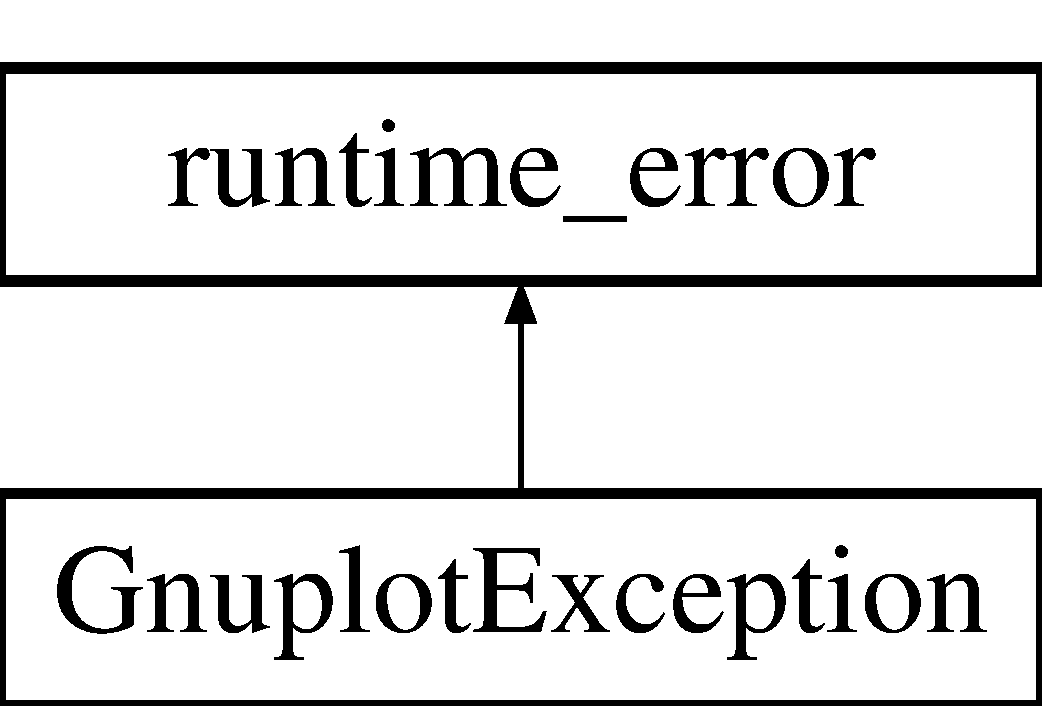
\includegraphics[height=2.000000cm]{class_gnuplot_exception}
\end{center}
\end{figure}
\subsection*{Public Member Functions}
\begin{DoxyCompactItemize}
\item 
\hypertarget{class_gnuplot_exception_a8b324a9ef4d3f75079d41ecd61c62d44}{{\bfseries Gnuplot\-Exception} (const std\-::string \&msg)}\label{class_gnuplot_exception_a8b324a9ef4d3f75079d41ecd61c62d44}

\end{DoxyCompactItemize}


\subsection{Detailed Description}
The interface uses pipes and so won't run on a system that doesn't have P\-O\-S\-I\-X pipe support Tested on Windows (Min\-G\-W and Visual C++) and Linux (G\-C\-C)

Version history\-: 0. C interface by N. Devillard (27/01/03)
\begin{DoxyEnumerate}
\item C++ interface\-: direct translation from the C interface by Rajarshi Guha (07/03/03)
\item corrections for Win32 compatibility by V. Chyzhdzenka (20/05/03)
\item some member functions added, corrections for Win32 and Linux compatibility by M. Burgis (10/03/08)
\item Some minor modifications to allow use by Key\-Cpp by J. Monschke (08/15/2013)
\end{DoxyEnumerate}

Requirements\-:
\begin{DoxyItemize}
\item gnuplot has to be installed (\href{http://www.gnuplot.info/download.html}{\tt http\-://www.\-gnuplot.\-info/download.\-html})
\item for Windows\-: set Path-\/\-Variable for \hyperlink{class_gnuplot}{Gnuplot} path (e.\-g. C\-:/program files/gnuplot/bin) or set \hyperlink{class_gnuplot}{Gnuplot} path with\-: \hyperlink{class_gnuplot_a67cae885c26ced821e335d98986f1967}{Gnuplot\-::set\-\_\-\-G\-N\-U\-Plot\-Path(const std\-::string \&path)}; 
\end{DoxyItemize}

The documentation for this class was generated from the following file\-:\begin{DoxyCompactItemize}
\item 
gnuplot\-\_\-i.\-h\end{DoxyCompactItemize}

\hypertarget{structboost_1_1numeric_1_1odeint_1_1is__resizeable_3_01keycpp_1_1matrix_3_01_t_00_011_01_4_01_4}{\section{boost\-:\-:numeric\-:\-:odeint\-:\-:is\-\_\-resizeable$<$ keycpp\-:\-:matrix$<$ T, 1 $>$ $>$ Struct Template Reference}
\label{structboost_1_1numeric_1_1odeint_1_1is__resizeable_3_01keycpp_1_1matrix_3_01_t_00_011_01_4_01_4}\index{boost\-::numeric\-::odeint\-::is\-\_\-resizeable$<$ keycpp\-::matrix$<$ T, 1 $>$ $>$@{boost\-::numeric\-::odeint\-::is\-\_\-resizeable$<$ keycpp\-::matrix$<$ T, 1 $>$ $>$}}
}
\subsection*{Public Types}
\begin{DoxyCompactItemize}
\item 
\hypertarget{structboost_1_1numeric_1_1odeint_1_1is__resizeable_3_01keycpp_1_1matrix_3_01_t_00_011_01_4_01_4_ace451c5d393b2ed47e601eb300832efd}{typedef boost\-::true\-\_\-type {\bfseries type}}\label{structboost_1_1numeric_1_1odeint_1_1is__resizeable_3_01keycpp_1_1matrix_3_01_t_00_011_01_4_01_4_ace451c5d393b2ed47e601eb300832efd}

\end{DoxyCompactItemize}
\subsection*{Static Public Attributes}
\begin{DoxyCompactItemize}
\item 
\hypertarget{structboost_1_1numeric_1_1odeint_1_1is__resizeable_3_01keycpp_1_1matrix_3_01_t_00_011_01_4_01_4_a16be7ca492a014298d22fc88ba5b2b84}{static const bool {\bfseries value} = type\-::value}\label{structboost_1_1numeric_1_1odeint_1_1is__resizeable_3_01keycpp_1_1matrix_3_01_t_00_011_01_4_01_4_a16be7ca492a014298d22fc88ba5b2b84}

\end{DoxyCompactItemize}


The documentation for this struct was generated from the following file\-:\begin{DoxyCompactItemize}
\item 
\hyperlink{keycpp_8h}{keycpp.\-h}\end{DoxyCompactItemize}

\hypertarget{classkeycpp_1_1_key_cpp_exception}{\section{keycpp\-:\-:Key\-Cpp\-Exception Class Reference}
\label{classkeycpp_1_1_key_cpp_exception}\index{keycpp\-::\-Key\-Cpp\-Exception@{keycpp\-::\-Key\-Cpp\-Exception}}
}
Inheritance diagram for keycpp\-:\-:Key\-Cpp\-Exception\-:\begin{figure}[H]
\begin{center}
\leavevmode
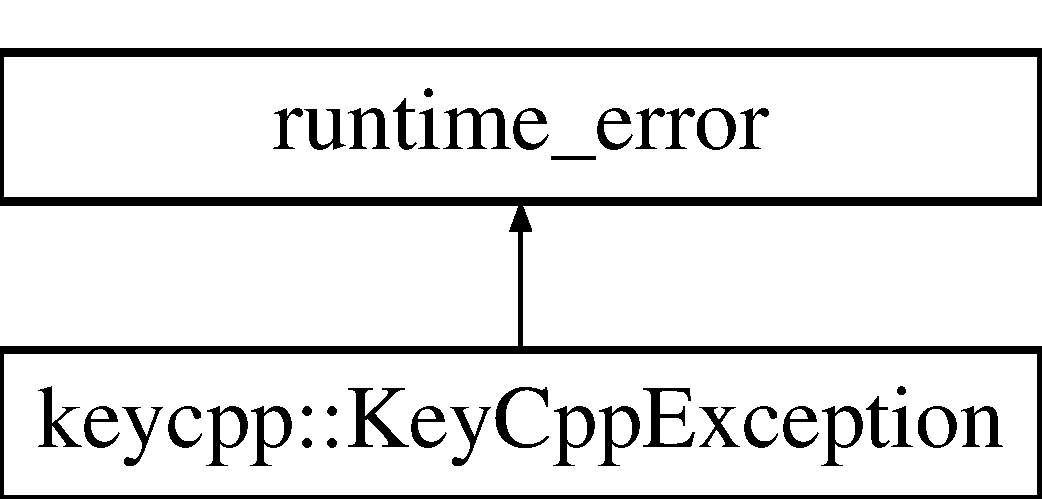
\includegraphics[height=2.000000cm]{classkeycpp_1_1_key_cpp_exception}
\end{center}
\end{figure}
\subsection*{Public Member Functions}
\begin{DoxyCompactItemize}
\item 
\hypertarget{classkeycpp_1_1_key_cpp_exception_af12dadc3f596f1e82cd65d55c2f64c65}{{\bfseries Key\-Cpp\-Exception} (const std\-::string \&msg)}\label{classkeycpp_1_1_key_cpp_exception_af12dadc3f596f1e82cd65d55c2f64c65}

\end{DoxyCompactItemize}


The documentation for this class was generated from the following file\-:\begin{DoxyCompactItemize}
\item 
\hyperlink{keycpp_8h}{keycpp.\-h}\end{DoxyCompactItemize}

\hypertarget{structkiss__fft__cpx}{\section{kiss\-\_\-fft\-\_\-cpx Struct Reference}
\label{structkiss__fft__cpx}\index{kiss\-\_\-fft\-\_\-cpx@{kiss\-\_\-fft\-\_\-cpx}}
}
\subsection*{Public Attributes}
\begin{DoxyCompactItemize}
\item 
\hypertarget{structkiss__fft__cpx_a686b6187e3e885de316908319c71ea8f}{kiss\-\_\-fft\-\_\-scalar {\bfseries r}}\label{structkiss__fft__cpx_a686b6187e3e885de316908319c71ea8f}

\item 
\hypertarget{structkiss__fft__cpx_ac1e17add2ae6b815da29d7d67b03fa70}{kiss\-\_\-fft\-\_\-scalar {\bfseries i}}\label{structkiss__fft__cpx_ac1e17add2ae6b815da29d7d67b03fa70}

\end{DoxyCompactItemize}


The documentation for this struct was generated from the following file\-:\begin{DoxyCompactItemize}
\item 
kiss\-\_\-fft.\-h\end{DoxyCompactItemize}

\hypertarget{structkiss__fft__state}{\section{kiss\-\_\-fft\-\_\-state Struct Reference}
\label{structkiss__fft__state}\index{kiss\-\_\-fft\-\_\-state@{kiss\-\_\-fft\-\_\-state}}
}
\subsection*{Public Attributes}
\begin{DoxyCompactItemize}
\item 
\hypertarget{structkiss__fft__state_aa7446bded329a40e13aef0826e349791}{int {\bfseries nfft}}\label{structkiss__fft__state_aa7446bded329a40e13aef0826e349791}

\item 
\hypertarget{structkiss__fft__state_a8faed935610ffb08bf7ad9ea8d6c81d2}{int {\bfseries inverse}}\label{structkiss__fft__state_a8faed935610ffb08bf7ad9ea8d6c81d2}

\item 
\hypertarget{structkiss__fft__state_a2d5d0897276dbac0674fae556f951d18}{int {\bfseries factors} \mbox{[}2 $\ast$M\-A\-X\-F\-A\-C\-T\-O\-R\-S\mbox{]}}\label{structkiss__fft__state_a2d5d0897276dbac0674fae556f951d18}

\item 
\hypertarget{structkiss__fft__state_aa7d1cab86ec03a8ecddfe0d91ef0bd20}{\hyperlink{structkiss__fft__cpx}{kiss\-\_\-fft\-\_\-cpx} {\bfseries twiddles} \mbox{[}1\mbox{]}}\label{structkiss__fft__state_aa7d1cab86ec03a8ecddfe0d91ef0bd20}

\end{DoxyCompactItemize}


The documentation for this struct was generated from the following file\-:\begin{DoxyCompactItemize}
\item 
\-\_\-kiss\-\_\-fft\-\_\-guts.\-h\end{DoxyCompactItemize}

\hypertarget{classkeycpp_1_1matrix}{\section{keycpp\-:\-:matrix$<$ T $>$ Class Template Reference}
\label{classkeycpp_1_1matrix}\index{keycpp\-::matrix$<$ T $>$@{keycpp\-::matrix$<$ T $>$}}
}
\subsection*{Public Member Functions}
\begin{DoxyCompactItemize}
\item 
\hypertarget{classkeycpp_1_1matrix_a7846ea93147dca75e5a8fbea7219c35d}{{\bfseries matrix} (const int \&rows, const int \&cols)}\label{classkeycpp_1_1matrix_a7846ea93147dca75e5a8fbea7219c35d}

\item 
\hypertarget{classkeycpp_1_1matrix_ad843813ecfec7c08b9259957406e94e2}{{\bfseries matrix} (const std\-::vector$<$ std\-::vector$<$ T $>$$>$ \&mat)}\label{classkeycpp_1_1matrix_ad843813ecfec7c08b9259957406e94e2}

\item 
\hypertarget{classkeycpp_1_1matrix_ad8797411bc30cc0d42e0e9b8bcc899d7}{{\bfseries matrix} (const std\-::initializer\-\_\-list$<$ std\-::initializer\-\_\-list$<$ T $>$$>$ \&lst)}\label{classkeycpp_1_1matrix_ad8797411bc30cc0d42e0e9b8bcc899d7}

\item 
\hypertarget{classkeycpp_1_1matrix_a9613f3ed2de6b240b982df895f958c56}{T \& {\bfseries operator()} (const int \&i, const int \&j)}\label{classkeycpp_1_1matrix_a9613f3ed2de6b240b982df895f958c56}

\item 
\hypertarget{classkeycpp_1_1matrix_a2c51fa98ec9a48f18af144677c36ee98}{T {\bfseries operator()} (const int \&i, const int \&j) const }\label{classkeycpp_1_1matrix_a2c51fa98ec9a48f18af144677c36ee98}

\item 
\hypertarget{classkeycpp_1_1matrix_a8a60e529610d6ad6ae5f34b8cd5199bd}{std\-::vector$<$ T $>$ {\bfseries operator$\ast$} (const std\-::vector$<$ T $>$ \&x) const }\label{classkeycpp_1_1matrix_a8a60e529610d6ad6ae5f34b8cd5199bd}

\item 
\hypertarget{classkeycpp_1_1matrix_add1f4ca03e1cce57574c905ab7ca89fe}{\hyperlink{classkeycpp_1_1matrix}{matrix}$<$ T $>$ {\bfseries operator$\ast$} (const \hyperlink{classkeycpp_1_1matrix}{matrix}$<$ T $>$ \&B) const }\label{classkeycpp_1_1matrix_add1f4ca03e1cce57574c905ab7ca89fe}

\item 
\hypertarget{classkeycpp_1_1matrix_a8c0520cf5064379afa5128cf7f660832}{\hyperlink{classkeycpp_1_1matrix}{matrix}$<$ T $>$ {\bfseries operator+} (const \hyperlink{classkeycpp_1_1matrix}{matrix}$<$ T $>$ \&B) const }\label{classkeycpp_1_1matrix_a8c0520cf5064379afa5128cf7f660832}

\item 
\hypertarget{classkeycpp_1_1matrix_a78655e73267b48e16909a68291f4c074}{\hyperlink{classkeycpp_1_1matrix}{matrix}$<$ T $>$ \& {\bfseries operator+=} (const \hyperlink{classkeycpp_1_1matrix}{matrix}$<$ T $>$ \&B)}\label{classkeycpp_1_1matrix_a78655e73267b48e16909a68291f4c074}

\item 
\hypertarget{classkeycpp_1_1matrix_a1c6cb00f8859e6486a7054f11b1c7e6a}{\hyperlink{classkeycpp_1_1matrix}{matrix}$<$ T $>$ {\bfseries operator-\/} (const \hyperlink{classkeycpp_1_1matrix}{matrix}$<$ T $>$ \&B) const }\label{classkeycpp_1_1matrix_a1c6cb00f8859e6486a7054f11b1c7e6a}

\item 
\hypertarget{classkeycpp_1_1matrix_a32a13ebb69fb5f06dd8923d942d865b4}{int {\bfseries size} (const int \&n) const }\label{classkeycpp_1_1matrix_a32a13ebb69fb5f06dd8923d942d865b4}

\item 
\hypertarget{classkeycpp_1_1matrix_ad522f701e86eafc344d8904d4f0a8f19}{bool {\bfseries empty} () const }\label{classkeycpp_1_1matrix_ad522f701e86eafc344d8904d4f0a8f19}

\item 
\hypertarget{classkeycpp_1_1matrix_a4b28c8f7b6e3d32aab1416faa9316e11}{int {\bfseries set\-Row} (const std\-::vector$<$ T $>$ \&row, const int \&i)}\label{classkeycpp_1_1matrix_a4b28c8f7b6e3d32aab1416faa9316e11}

\item 
\hypertarget{classkeycpp_1_1matrix_ac7675f496771e688a1c059b58ac975cb}{int {\bfseries set\-Last\-Row} (const std\-::vector$<$ T $>$ \&row)}\label{classkeycpp_1_1matrix_ac7675f496771e688a1c059b58ac975cb}

\item 
\hypertarget{classkeycpp_1_1matrix_aa6903fc828a5b42f7c1d9485832601aa}{int {\bfseries add\-Last\-Row} (const std\-::vector$<$ T $>$ \&row)}\label{classkeycpp_1_1matrix_aa6903fc828a5b42f7c1d9485832601aa}

\item 
\hypertarget{classkeycpp_1_1matrix_adf4d81176c098ead33c56d84421b14f5}{int {\bfseries set\-Col} (const std\-::vector$<$ T $>$ \&col, const int \&j)}\label{classkeycpp_1_1matrix_adf4d81176c098ead33c56d84421b14f5}

\item 
\hypertarget{classkeycpp_1_1matrix_a14cad5ff7a9b3079754fc83b677208ed}{std\-::vector$<$ T $>$ {\bfseries get\-Row} (const int \&i) const }\label{classkeycpp_1_1matrix_a14cad5ff7a9b3079754fc83b677208ed}

\item 
\hypertarget{classkeycpp_1_1matrix_a20002e97217bcc6382e60694bf898e1f}{std\-::vector$<$ T $>$ {\bfseries get\-Last\-Row} () const }\label{classkeycpp_1_1matrix_a20002e97217bcc6382e60694bf898e1f}

\item 
\hypertarget{classkeycpp_1_1matrix_a9c16ead5c2a61eb35c33328caa235b2f}{std\-::vector$<$ T $>$ {\bfseries get\-Col} (const int \&j) const }\label{classkeycpp_1_1matrix_a9c16ead5c2a61eb35c33328caa235b2f}

\item 
\hypertarget{classkeycpp_1_1matrix_a719eb1cb62d0cd9168abe2235235f278}{int {\bfseries reserve} (const int \&N)}\label{classkeycpp_1_1matrix_a719eb1cb62d0cd9168abe2235235f278}

\item 
\hypertarget{classkeycpp_1_1matrix_a53aaf4f54bdbebf5664b67a440f73040}{{\footnotesize template$<$$>$ }\\std\-::vector$<$ double $>$ {\bfseries operator$\ast$} (const std\-::vector$<$ double $>$ \&x) const}\label{classkeycpp_1_1matrix_a53aaf4f54bdbebf5664b67a440f73040}

\item 
\hypertarget{classkeycpp_1_1matrix_a8a9131597beafc39a3d94b59af930756}{{\footnotesize template$<$$>$ }\\std\-::vector$<$ std\-::complex\\*
$<$ double $>$ $>$ {\bfseries operator$\ast$} (const std\-::vector$<$ std\-::complex$<$ double $>$$>$ \&x) const}\label{classkeycpp_1_1matrix_a8a9131597beafc39a3d94b59af930756}

\item 
\hypertarget{classkeycpp_1_1matrix_a0e9fdbebdf1d95dd225a2bd1310cba30}{{\footnotesize template$<$$>$ }\\\hyperlink{classkeycpp_1_1matrix}{matrix}$<$ double $>$ {\bfseries operator$\ast$} (const \hyperlink{classkeycpp_1_1matrix}{matrix}$<$ double $>$ \&B) const}\label{classkeycpp_1_1matrix_a0e9fdbebdf1d95dd225a2bd1310cba30}

\item 
\hypertarget{classkeycpp_1_1matrix_a0cbaef09170a16f74ed5acefa0f8ad3a}{{\footnotesize template$<$$>$ }\\\hyperlink{classkeycpp_1_1matrix}{matrix}$<$ std\-::complex$<$ double $>$ $>$ {\bfseries operator$\ast$} (const \hyperlink{classkeycpp_1_1matrix}{matrix}$<$ std\-::complex$<$ double $>$$>$ \&B) const}\label{classkeycpp_1_1matrix_a0cbaef09170a16f74ed5acefa0f8ad3a}

\end{DoxyCompactItemize}
\subsection*{Public Attributes}
\begin{DoxyCompactItemize}
\item 
\hypertarget{classkeycpp_1_1matrix_ae2144abe57757c5a29e73aaf4d3520aa}{std\-::vector$<$ T $>$ {\bfseries m\-Data}}\label{classkeycpp_1_1matrix_ae2144abe57757c5a29e73aaf4d3520aa}

\end{DoxyCompactItemize}


The documentation for this class was generated from the following file\-:\begin{DoxyCompactItemize}
\item 
Matrix.\-h\end{DoxyCompactItemize}

\hypertarget{structkeycpp_1_1matrix__find__type}{\section{keycpp\-:\-:matrix\-\_\-find\-\_\-type$<$ T $>$ Struct Template Reference}
\label{structkeycpp_1_1matrix__find__type}\index{keycpp\-::matrix\-\_\-find\-\_\-type$<$ T $>$@{keycpp\-::matrix\-\_\-find\-\_\-type$<$ T $>$}}
}
\subsection*{Public Attributes}
\begin{DoxyCompactItemize}
\item 
\hypertarget{structkeycpp_1_1matrix__find__type_a34ca318ae96bc18fe29ac2a42ab1b520}{std\-::vector$<$ int $>$ {\bfseries rows}}\label{structkeycpp_1_1matrix__find__type_a34ca318ae96bc18fe29ac2a42ab1b520}

\item 
\hypertarget{structkeycpp_1_1matrix__find__type_a034a9a0159b07d68cdc688e36648667c}{std\-::vector$<$ int $>$ {\bfseries cols}}\label{structkeycpp_1_1matrix__find__type_a034a9a0159b07d68cdc688e36648667c}

\item 
\hypertarget{structkeycpp_1_1matrix__find__type_a46d32e3990c9333dbbfc77adece4159b}{std\-::vector$<$ T $>$ {\bfseries v}}\label{structkeycpp_1_1matrix__find__type_a46d32e3990c9333dbbfc77adece4159b}

\end{DoxyCompactItemize}


The documentation for this struct was generated from the following file\-:\begin{DoxyCompactItemize}
\item 
\hyperlink{keycpp_8h}{keycpp.\-h}\end{DoxyCompactItemize}

\hypertarget{classkeycpp_1_1_matrix_exception}{\section{keycpp\-:\-:Matrix\-Exception Class Reference}
\label{classkeycpp_1_1_matrix_exception}\index{keycpp\-::\-Matrix\-Exception@{keycpp\-::\-Matrix\-Exception}}
}
Inheritance diagram for keycpp\-:\-:Matrix\-Exception\-:\begin{figure}[H]
\begin{center}
\leavevmode
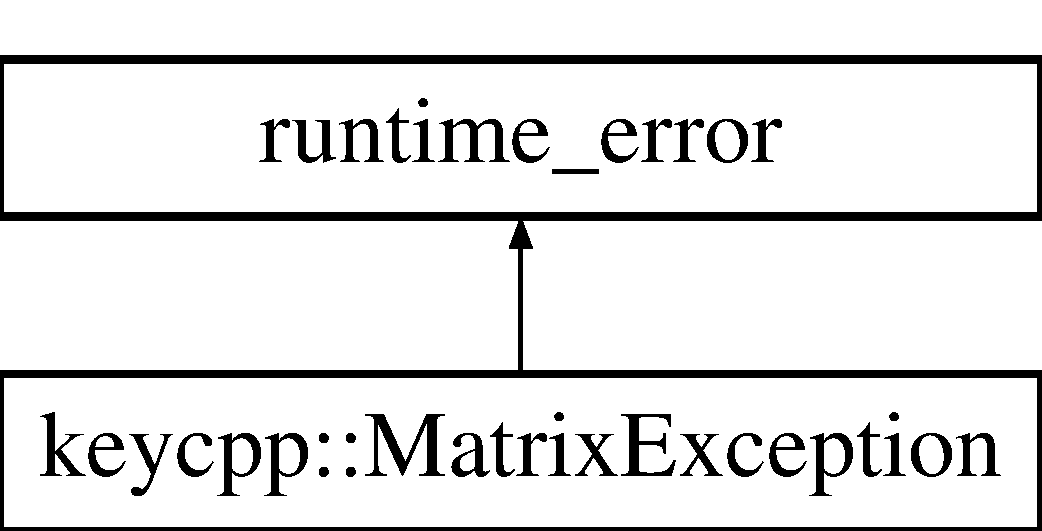
\includegraphics[height=2.000000cm]{classkeycpp_1_1_matrix_exception}
\end{center}
\end{figure}
\subsection*{Public Member Functions}
\begin{DoxyCompactItemize}
\item 
\hypertarget{classkeycpp_1_1_matrix_exception_ae558e1658f52404739cbb6fe784f196d}{{\bfseries Matrix\-Exception} (const std\-::string \&msg)}\label{classkeycpp_1_1_matrix_exception_ae558e1658f52404739cbb6fe784f196d}

\end{DoxyCompactItemize}


The documentation for this class was generated from the following file\-:\begin{DoxyCompactItemize}
\item 
Matrix.\-h\end{DoxyCompactItemize}

\hypertarget{structkeycpp_1_1observe}{\section{keycpp\-:\-:observe$<$ T, U $>$ Struct Template Reference}
\label{structkeycpp_1_1observe}\index{keycpp\-::observe$<$ T, U $>$@{keycpp\-::observe$<$ T, U $>$}}
}
\subsection*{Public Member Functions}
\begin{DoxyCompactItemize}
\item 
\hypertarget{structkeycpp_1_1observe_a88747e0078d06440401d309aba55954e}{{\bfseries observe} (std\-::vector$<$ T $>$ \&p\-\_\-y, std\-::vector$<$ U $>$ \&p\-\_\-x\-\_\-ode)}\label{structkeycpp_1_1observe_a88747e0078d06440401d309aba55954e}

\item 
\hypertarget{structkeycpp_1_1observe_a0063ab6fcada5756c6dca31ac7c17af9}{void {\bfseries operator()} (const T \&y\-\_\-temp, U x\-\_\-temp)}\label{structkeycpp_1_1observe_a0063ab6fcada5756c6dca31ac7c17af9}

\end{DoxyCompactItemize}
\subsection*{Public Attributes}
\begin{DoxyCompactItemize}
\item 
\hypertarget{structkeycpp_1_1observe_ab864306595f62009949934d352b43abf}{std\-::vector$<$ T $>$ \& {\bfseries y}}\label{structkeycpp_1_1observe_ab864306595f62009949934d352b43abf}

\item 
\hypertarget{structkeycpp_1_1observe_aecc1e14f64f33f35c50aee35cc86dac5}{std\-::vector$<$ U $>$ \& {\bfseries x\-\_\-ode}}\label{structkeycpp_1_1observe_aecc1e14f64f33f35c50aee35cc86dac5}

\end{DoxyCompactItemize}


The documentation for this struct was generated from the following file\-:\begin{DoxyCompactItemize}
\item 
keycpp.\-h\end{DoxyCompactItemize}

\hypertarget{structkeycpp_1_1_o_d_e__type}{\section{keycpp\-:\-:O\-D\-E\-\_\-type$<$ T, Y $>$ Struct Template Reference}
\label{structkeycpp_1_1_o_d_e__type}\index{keycpp\-::\-O\-D\-E\-\_\-type$<$ T, Y $>$@{keycpp\-::\-O\-D\-E\-\_\-type$<$ T, Y $>$}}
}
\subsection*{Public Attributes}
\begin{DoxyCompactItemize}
\item 
\hypertarget{structkeycpp_1_1_o_d_e__type_a7472927d5cc31aaf06d8dd1024b7640e}{\hyperlink{classkeycpp_1_1matrix}{matrix}$<$ T, 2 $>$ {\bfseries t}}\label{structkeycpp_1_1_o_d_e__type_a7472927d5cc31aaf06d8dd1024b7640e}

\item 
\hypertarget{structkeycpp_1_1_o_d_e__type_aafb0eeede0354cc546c0114ef3c15129}{\hyperlink{classkeycpp_1_1matrix}{matrix}$<$ Y, 2 $>$ {\bfseries y}}\label{structkeycpp_1_1_o_d_e__type_aafb0eeede0354cc546c0114ef3c15129}

\end{DoxyCompactItemize}


The documentation for this struct was generated from the following file\-:\begin{DoxyCompactItemize}
\item 
\hyperlink{keycpp_8h}{keycpp.\-h}\end{DoxyCompactItemize}

\hypertarget{class_ode_class}{\section{Ode\-Class Class Reference}
\label{class_ode_class}\index{Ode\-Class@{Ode\-Class}}
}
\subsection*{Public Member Functions}
\begin{DoxyCompactItemize}
\item 
\hypertarget{class_ode_class_a1c4fbb90c42265ba4e81664a192f1d8f}{void {\bfseries operator()} (const \hyperlink{classkeycpp_1_1matrix}{matrix}$<$ double $>$ \&y, \hyperlink{classkeycpp_1_1matrix}{matrix}$<$ double $>$ \&dy, const double)}\label{class_ode_class_a1c4fbb90c42265ba4e81664a192f1d8f}

\item 
\hypertarget{class_ode_class_a269b7862197785ff7c52d453cfa0b98e}{void {\bfseries operator()} (const \hyperlink{classkeycpp_1_1matrix}{keycpp\-::matrix}$<$ double, 2 $>$ \&y, \hyperlink{classkeycpp_1_1matrix}{keycpp\-::matrix}$<$ double, 2 $>$ \&dy, const double t)}\label{class_ode_class_a269b7862197785ff7c52d453cfa0b98e}

\end{DoxyCompactItemize}


The documentation for this class was generated from the following files\-:\begin{DoxyCompactItemize}
\item 
example.\-cpp\item 
test\-\_\-ode45.\-cpp\end{DoxyCompactItemize}

\hypertarget{classkeycpp_1_1_plots}{\section{keycpp\-:\-:Plots Class Reference}
\label{classkeycpp_1_1_plots}\index{keycpp\-::\-Plots@{keycpp\-::\-Plots}}
}
\subsection*{Public Attributes}
\begin{DoxyCompactItemize}
\item 
\hypertarget{classkeycpp_1_1_plots_afe961c1f35d88bc181bd426fc47ade00}{bool {\bfseries hold\-\_\-on\-\_\-bool} = false}\label{classkeycpp_1_1_plots_afe961c1f35d88bc181bd426fc47ade00}

\item 
\hypertarget{classkeycpp_1_1_plots_aa37e3813d1a29d423700af686dc1bf09}{int {\bfseries num\-\_\-plots} = 0}\label{classkeycpp_1_1_plots_aa37e3813d1a29d423700af686dc1bf09}

\item 
\hypertarget{classkeycpp_1_1_plots_a9de0b584d162d6694ea4281cb9a4396d}{std\-::vector$<$ std\-::vector\\*
$<$ double $>$ $>$ {\bfseries x\-\_\-plot\-\_\-data}}\label{classkeycpp_1_1_plots_a9de0b584d162d6694ea4281cb9a4396d}

\item 
\hypertarget{classkeycpp_1_1_plots_a3f3f95d6306139576d53734972995720}{std\-::vector$<$ std\-::vector\\*
$<$ double $>$ $>$ {\bfseries y\-\_\-plot\-\_\-data}}\label{classkeycpp_1_1_plots_a3f3f95d6306139576d53734972995720}

\item 
\hypertarget{classkeycpp_1_1_plots_a462b8a89f01d8beb747ec82a85530e3a}{std\-::vector$<$ std\-::string $>$ {\bfseries plot\-\_\-format}}\label{classkeycpp_1_1_plots_a462b8a89f01d8beb747ec82a85530e3a}

\item 
\hypertarget{classkeycpp_1_1_plots_a3d01b697171789f31c7e77764c905216}{std\-::vector$<$ double $>$ {\bfseries plot\-\_\-linewidth}}\label{classkeycpp_1_1_plots_a3d01b697171789f31c7e77764c905216}

\item 
\hypertarget{classkeycpp_1_1_plots_ad801040d683566ecf22c3c1ec72e6811}{std\-::vector$<$ double $>$ {\bfseries plot\-\_\-markersize}}\label{classkeycpp_1_1_plots_ad801040d683566ecf22c3c1ec72e6811}

\item 
\hypertarget{classkeycpp_1_1_plots_a95cfb5daf2425e227f5148c7c6a04e80}{std\-::vector$<$ double $>$ {\bfseries plot\-\_\-val}}\label{classkeycpp_1_1_plots_a95cfb5daf2425e227f5148c7c6a04e80}

\item 
\hypertarget{classkeycpp_1_1_plots_a25df6878ccfbbe680c5324e0fab789ac}{std\-::vector$<$ std\-::string $>$ {\bfseries legend\-\_\-entries}}\label{classkeycpp_1_1_plots_a25df6878ccfbbe680c5324e0fab789ac}

\item 
\hypertarget{classkeycpp_1_1_plots_add620558a2e9a243a95ffdfe7489897b}{std\-::string {\bfseries legend\-\_\-location} = \char`\"{}ins vert right top\char`\"{}}\label{classkeycpp_1_1_plots_add620558a2e9a243a95ffdfe7489897b}

\item 
\hypertarget{classkeycpp_1_1_plots_ab3c932242df0fa03798ecfd2dba3ebaa}{std\-::string {\bfseries legend\-\_\-box} = \char`\"{} box\char`\"{}}\label{classkeycpp_1_1_plots_ab3c932242df0fa03798ecfd2dba3ebaa}

\item 
\hypertarget{classkeycpp_1_1_plots_a18a69c533594b4bc1c88fdb29267db1e}{std\-::string {\bfseries m\-\_\-xlabel}}\label{classkeycpp_1_1_plots_a18a69c533594b4bc1c88fdb29267db1e}

\item 
\hypertarget{classkeycpp_1_1_plots_ad2987af367059a0659e013708342451b}{std\-::string {\bfseries m\-\_\-ylabel}}\label{classkeycpp_1_1_plots_ad2987af367059a0659e013708342451b}

\item 
\hypertarget{classkeycpp_1_1_plots_a849d297c44ebca4f7c856c99cfcc2b5f}{std\-::string {\bfseries m\-\_\-title}}\label{classkeycpp_1_1_plots_a849d297c44ebca4f7c856c99cfcc2b5f}

\item 
\hypertarget{classkeycpp_1_1_plots_a54578198c41d34705e9fbe94a88ec6ae}{double {\bfseries ymin}}\label{classkeycpp_1_1_plots_a54578198c41d34705e9fbe94a88ec6ae}

\item 
\hypertarget{classkeycpp_1_1_plots_ad411158572c6ee36b1f4abc9c9dfec77}{double {\bfseries ymax}}\label{classkeycpp_1_1_plots_ad411158572c6ee36b1f4abc9c9dfec77}

\item 
\hypertarget{classkeycpp_1_1_plots_a1d027ed119d5b4a8d7d9ccc72f9a0eb1}{double {\bfseries xmin}}\label{classkeycpp_1_1_plots_a1d027ed119d5b4a8d7d9ccc72f9a0eb1}

\item 
\hypertarget{classkeycpp_1_1_plots_a4d7f34173d13de92014702ffba6fb1d4}{double {\bfseries xmax}}\label{classkeycpp_1_1_plots_a4d7f34173d13de92014702ffba6fb1d4}

\item 
\hypertarget{classkeycpp_1_1_plots_abd0c4449bcd999429a3073e2885708d8}{bool {\bfseries grid\-\_\-on\-\_\-bool} = false}\label{classkeycpp_1_1_plots_abd0c4449bcd999429a3073e2885708d8}

\item 
\hypertarget{classkeycpp_1_1_plots_aa994c8e9f09633b26410ed27ea70a1a1}{bool {\bfseries logscale\-\_\-x} = false}\label{classkeycpp_1_1_plots_aa994c8e9f09633b26410ed27ea70a1a1}

\item 
\hypertarget{classkeycpp_1_1_plots_a605e7e4681e977f5d1d2ff95d72946cb}{bool {\bfseries logscale\-\_\-y} = false}\label{classkeycpp_1_1_plots_a605e7e4681e977f5d1d2ff95d72946cb}

\item 
\hypertarget{classkeycpp_1_1_plots_a0ed0add050a618468cbf2cffe2529bad}{std\-::ostringstream {\bfseries cmdstr}}\label{classkeycpp_1_1_plots_a0ed0add050a618468cbf2cffe2529bad}

\end{DoxyCompactItemize}


The documentation for this class was generated from the following file\-:\begin{DoxyCompactItemize}
\item 
Figure.\-h\end{DoxyCompactItemize}

\hypertarget{classkeycpp_1_1_pointer_iterator}{\section{keycpp\-:\-:Pointer\-Iterator$<$ Type\-T $>$ Class Template Reference}
\label{classkeycpp_1_1_pointer_iterator}\index{keycpp\-::\-Pointer\-Iterator$<$ Type\-T $>$@{keycpp\-::\-Pointer\-Iterator$<$ Type\-T $>$}}
}
Inheritance diagram for keycpp\-:\-:Pointer\-Iterator$<$ Type\-T $>$\-:\begin{figure}[H]
\begin{center}
\leavevmode
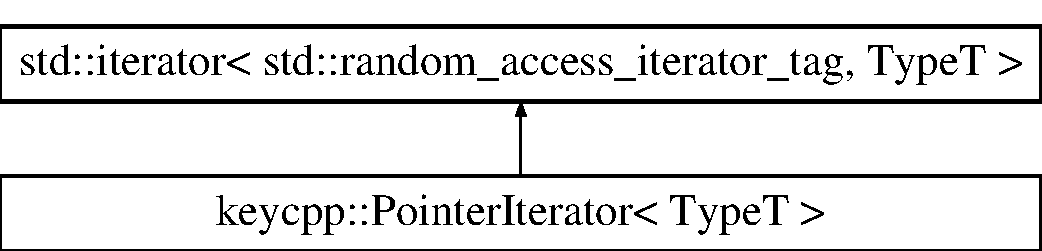
\includegraphics[height=2.000000cm]{classkeycpp_1_1_pointer_iterator}
\end{center}
\end{figure}
\subsection*{Public Types}
\begin{DoxyCompactItemize}
\item 
\hypertarget{classkeycpp_1_1_pointer_iterator_a1ef73c2e3452ec372b1bcc67e4d32fa6}{typedef \\*
std\-::random\-\_\-access\-\_\-iterator\-\_\-tag {\bfseries iterator\-\_\-category}}\label{classkeycpp_1_1_pointer_iterator_a1ef73c2e3452ec372b1bcc67e4d32fa6}

\item 
\hypertarget{classkeycpp_1_1_pointer_iterator_a5cd2295724a4697502177353b7d1f8cf}{typedef std\-::iterator\\*
$<$ std\-::random\-\_\-access\-\_\-iterator\-\_\-tag, \\*
Type\-T $>$\-::value\-\_\-type {\bfseries value\-\_\-type}}\label{classkeycpp_1_1_pointer_iterator_a5cd2295724a4697502177353b7d1f8cf}

\item 
\hypertarget{classkeycpp_1_1_pointer_iterator_afe9aba481fceabc3ff98dfd05591e199}{typedef std\-::iterator\\*
$<$ std\-::random\-\_\-access\-\_\-iterator\-\_\-tag, \\*
Type\-T $>$\-::difference\-\_\-type {\bfseries difference\-\_\-type}}\label{classkeycpp_1_1_pointer_iterator_afe9aba481fceabc3ff98dfd05591e199}

\item 
\hypertarget{classkeycpp_1_1_pointer_iterator_afb9ff3879d195f7361980a126756ebc0}{typedef std\-::iterator\\*
$<$ std\-::random\-\_\-access\-\_\-iterator\-\_\-tag, \\*
Type\-T $>$\-::reference {\bfseries reference}}\label{classkeycpp_1_1_pointer_iterator_afb9ff3879d195f7361980a126756ebc0}

\item 
\hypertarget{classkeycpp_1_1_pointer_iterator_adada9309981bd33390b4b461c8f5b853}{typedef std\-::iterator\\*
$<$ std\-::random\-\_\-access\-\_\-iterator\-\_\-tag, \\*
Type\-T $>$\-::pointer {\bfseries pointer}}\label{classkeycpp_1_1_pointer_iterator_adada9309981bd33390b4b461c8f5b853}

\end{DoxyCompactItemize}
\subsection*{Public Member Functions}
\begin{DoxyCompactItemize}
\item 
\hypertarget{classkeycpp_1_1_pointer_iterator_a8144990606b147959521783cc7a7934f}{{\footnotesize template$<$typename T2 $>$ }\\{\bfseries Pointer\-Iterator} (const \hyperlink{classkeycpp_1_1_pointer_iterator}{Pointer\-Iterator}$<$ T2 $>$ \&r)}\label{classkeycpp_1_1_pointer_iterator_a8144990606b147959521783cc7a7934f}

\item 
\hypertarget{classkeycpp_1_1_pointer_iterator_aa1a5f134d80ade0a24b6232f25d81a52}{{\bfseries Pointer\-Iterator} (pointer p\-Data, size\-\_\-t pinc=1)}\label{classkeycpp_1_1_pointer_iterator_aa1a5f134d80ade0a24b6232f25d81a52}

\item 
\hypertarget{classkeycpp_1_1_pointer_iterator_aac3906d9cdca051a792ef7899f78d47a}{{\footnotesize template$<$typename T2 $>$ }\\\hyperlink{classkeycpp_1_1_pointer_iterator}{Pointer\-Iterator} \& {\bfseries operator=} (const \hyperlink{classkeycpp_1_1_pointer_iterator}{Pointer\-Iterator}$<$ T2 $>$ \&r)}\label{classkeycpp_1_1_pointer_iterator_aac3906d9cdca051a792ef7899f78d47a}

\item 
\hypertarget{classkeycpp_1_1_pointer_iterator_adb5f11092924ec2ffdb0987221ac09f7}{\hyperlink{classkeycpp_1_1_pointer_iterator}{Pointer\-Iterator} \& {\bfseries operator++} ()}\label{classkeycpp_1_1_pointer_iterator_adb5f11092924ec2ffdb0987221ac09f7}

\item 
\hypertarget{classkeycpp_1_1_pointer_iterator_a8817b17c51afe87381ea2911386d2210}{\hyperlink{classkeycpp_1_1_pointer_iterator}{Pointer\-Iterator} \& {\bfseries operator-\/-\/} ()}\label{classkeycpp_1_1_pointer_iterator_a8817b17c51afe87381ea2911386d2210}

\item 
\hypertarget{classkeycpp_1_1_pointer_iterator_a84bfd964409dfdf89343cc9db3e996df}{\hyperlink{classkeycpp_1_1_pointer_iterator}{Pointer\-Iterator} {\bfseries operator++} (int)}\label{classkeycpp_1_1_pointer_iterator_a84bfd964409dfdf89343cc9db3e996df}

\item 
\hypertarget{classkeycpp_1_1_pointer_iterator_ac4da97a9c8c09ad6ee1d27f4eb27310f}{\hyperlink{classkeycpp_1_1_pointer_iterator}{Pointer\-Iterator} {\bfseries operator-\/-\/} (int)}\label{classkeycpp_1_1_pointer_iterator_ac4da97a9c8c09ad6ee1d27f4eb27310f}

\item 
\hypertarget{classkeycpp_1_1_pointer_iterator_a93d3314a1e2896d39b87fce1c79cf3c0}{\hyperlink{classkeycpp_1_1_pointer_iterator}{Pointer\-Iterator} {\bfseries operator+} (const difference\-\_\-type \&n) const }\label{classkeycpp_1_1_pointer_iterator_a93d3314a1e2896d39b87fce1c79cf3c0}

\item 
\hypertarget{classkeycpp_1_1_pointer_iterator_a3cc779696b1e9b2c9aff80608ade1fce}{\hyperlink{classkeycpp_1_1_pointer_iterator}{Pointer\-Iterator} \& {\bfseries operator+=} (const difference\-\_\-type \&n)}\label{classkeycpp_1_1_pointer_iterator_a3cc779696b1e9b2c9aff80608ade1fce}

\item 
\hypertarget{classkeycpp_1_1_pointer_iterator_a30dbe9e2a35428de230bc91989ef36dd}{\hyperlink{classkeycpp_1_1_pointer_iterator}{Pointer\-Iterator} {\bfseries operator-\/} (const difference\-\_\-type \&n) const }\label{classkeycpp_1_1_pointer_iterator_a30dbe9e2a35428de230bc91989ef36dd}

\item 
\hypertarget{classkeycpp_1_1_pointer_iterator_a070e0ded5d9a1e27a81beef460e56dc1}{\hyperlink{classkeycpp_1_1_pointer_iterator}{Pointer\-Iterator} \& {\bfseries operator-\/=} (const difference\-\_\-type \&n)}\label{classkeycpp_1_1_pointer_iterator_a070e0ded5d9a1e27a81beef460e56dc1}

\item 
\hypertarget{classkeycpp_1_1_pointer_iterator_a8f90f761a85a25dc17e6c4c1a3d395c9}{reference {\bfseries operator$\ast$} () const }\label{classkeycpp_1_1_pointer_iterator_a8f90f761a85a25dc17e6c4c1a3d395c9}

\item 
\hypertarget{classkeycpp_1_1_pointer_iterator_ae43cd45245f9d970256e1b3f021f3d53}{pointer {\bfseries operator-\/$>$} () const }\label{classkeycpp_1_1_pointer_iterator_ae43cd45245f9d970256e1b3f021f3d53}

\item 
\hypertarget{classkeycpp_1_1_pointer_iterator_a390b37fc74ce6893512e8a02c4fea83d}{reference {\bfseries operator\mbox{[}$\,$\mbox{]}} (const difference\-\_\-type \&n) const }\label{classkeycpp_1_1_pointer_iterator_a390b37fc74ce6893512e8a02c4fea83d}

\item 
\hypertarget{classkeycpp_1_1_pointer_iterator_a52500cdd636c14af6f85196b1cae8a44}{size\-\_\-t {\bfseries get\-\_\-inc} () const }\label{classkeycpp_1_1_pointer_iterator_a52500cdd636c14af6f85196b1cae8a44}

\end{DoxyCompactItemize}
\subsection*{Protected Attributes}
\begin{DoxyCompactItemize}
\item 
\hypertarget{classkeycpp_1_1_pointer_iterator_ad513bffb30233c61f684a8e8e1d0ab53}{Type\-T $\ast$ {\bfseries m\-\_\-p\-Data}}\label{classkeycpp_1_1_pointer_iterator_ad513bffb30233c61f684a8e8e1d0ab53}

\item 
\hypertarget{classkeycpp_1_1_pointer_iterator_ae2e20193e310cd9fc439a5ef7a949295}{size\-\_\-t {\bfseries inc}}\label{classkeycpp_1_1_pointer_iterator_ae2e20193e310cd9fc439a5ef7a949295}

\end{DoxyCompactItemize}
\subsection*{Friends}
\begin{DoxyCompactItemize}
\item 
\hypertarget{classkeycpp_1_1_pointer_iterator_a06dfe074dcfe7a2ab9527586369dbcc3}{{\footnotesize template$<$typename T $>$ }\\bool {\bfseries operator==} (const \hyperlink{classkeycpp_1_1_pointer_iterator}{Pointer\-Iterator}$<$ T $>$ \&r1, const \hyperlink{classkeycpp_1_1_pointer_iterator}{Pointer\-Iterator}$<$ T $>$ \&r2)}\label{classkeycpp_1_1_pointer_iterator_a06dfe074dcfe7a2ab9527586369dbcc3}

\item 
\hypertarget{classkeycpp_1_1_pointer_iterator_a7682ba01e82b3aba962c6ee0c32d4d3d}{{\footnotesize template$<$typename T $>$ }\\bool {\bfseries operator!=} (const \hyperlink{classkeycpp_1_1_pointer_iterator}{Pointer\-Iterator}$<$ T $>$ \&r1, const \hyperlink{classkeycpp_1_1_pointer_iterator}{Pointer\-Iterator}$<$ T $>$ \&r2)}\label{classkeycpp_1_1_pointer_iterator_a7682ba01e82b3aba962c6ee0c32d4d3d}

\item 
\hypertarget{classkeycpp_1_1_pointer_iterator_af558be7c8449cd575bbf7b362d27b6f9}{{\footnotesize template$<$typename T $>$ }\\bool {\bfseries operator$<$} (const \hyperlink{classkeycpp_1_1_pointer_iterator}{Pointer\-Iterator}$<$ T $>$ \&r1, const \hyperlink{classkeycpp_1_1_pointer_iterator}{Pointer\-Iterator}$<$ T $>$ \&r2)}\label{classkeycpp_1_1_pointer_iterator_af558be7c8449cd575bbf7b362d27b6f9}

\item 
\hypertarget{classkeycpp_1_1_pointer_iterator_a29c4edb27dcc46bea93df78eef3eb1f7}{{\footnotesize template$<$typename T $>$ }\\bool {\bfseries operator$>$} (const \hyperlink{classkeycpp_1_1_pointer_iterator}{Pointer\-Iterator}$<$ T $>$ \&r1, const \hyperlink{classkeycpp_1_1_pointer_iterator}{Pointer\-Iterator}$<$ T $>$ \&r2)}\label{classkeycpp_1_1_pointer_iterator_a29c4edb27dcc46bea93df78eef3eb1f7}

\item 
\hypertarget{classkeycpp_1_1_pointer_iterator_afc6f64c3c35e55197f846b2328cb21f8}{{\footnotesize template$<$typename T $>$ }\\bool {\bfseries operator$<$=} (const \hyperlink{classkeycpp_1_1_pointer_iterator}{Pointer\-Iterator}$<$ T $>$ \&r1, const \hyperlink{classkeycpp_1_1_pointer_iterator}{Pointer\-Iterator}$<$ T $>$ \&r2)}\label{classkeycpp_1_1_pointer_iterator_afc6f64c3c35e55197f846b2328cb21f8}

\item 
\hypertarget{classkeycpp_1_1_pointer_iterator_a7a58bf216a9bd8b4a4cfd2905a421b8c}{{\footnotesize template$<$typename T $>$ }\\bool {\bfseries operator$>$=} (const \hyperlink{classkeycpp_1_1_pointer_iterator}{Pointer\-Iterator}$<$ T $>$ \&r1, const \hyperlink{classkeycpp_1_1_pointer_iterator}{Pointer\-Iterator}$<$ T $>$ \&r2)}\label{classkeycpp_1_1_pointer_iterator_a7a58bf216a9bd8b4a4cfd2905a421b8c}

\item 
\hypertarget{classkeycpp_1_1_pointer_iterator_a8e7bea4d56f15979b01078c740fc9d33}{{\footnotesize template$<$typename T $>$ }\\\hyperlink{classkeycpp_1_1_pointer_iterator}{Pointer\-Iterator}$<$ T $>$\\*
\-::difference\-\_\-type {\bfseries operator+} (const \hyperlink{classkeycpp_1_1_pointer_iterator}{Pointer\-Iterator}$<$ T $>$ \&r1, const \hyperlink{classkeycpp_1_1_pointer_iterator}{Pointer\-Iterator}$<$ T $>$ \&r2)}\label{classkeycpp_1_1_pointer_iterator_a8e7bea4d56f15979b01078c740fc9d33}

\item 
\hypertarget{classkeycpp_1_1_pointer_iterator_a0c82b8711579ffa15e4ec6f8952e7bda}{{\footnotesize template$<$typename T $>$ }\\\hyperlink{classkeycpp_1_1_pointer_iterator}{Pointer\-Iterator}$<$ T $>$\\*
\-::difference\-\_\-type {\bfseries operator-\/} (const \hyperlink{classkeycpp_1_1_pointer_iterator}{Pointer\-Iterator}$<$ T $>$ \&r1, const \hyperlink{classkeycpp_1_1_pointer_iterator}{Pointer\-Iterator}$<$ T $>$ \&r2)}\label{classkeycpp_1_1_pointer_iterator_a0c82b8711579ffa15e4ec6f8952e7bda}

\end{DoxyCompactItemize}


The documentation for this class was generated from the following file\-:\begin{DoxyCompactItemize}
\item 
vector\-\_\-k.\-h\end{DoxyCompactItemize}

\hypertarget{structkeycpp_1_1_sort___matrix}{\section{keycpp\-:\-:Sort\-\_\-\-Matrix$<$ T $>$ Struct Template Reference}
\label{structkeycpp_1_1_sort___matrix}\index{keycpp\-::\-Sort\-\_\-\-Matrix$<$ T $>$@{keycpp\-::\-Sort\-\_\-\-Matrix$<$ T $>$}}
}
\subsection*{Public Attributes}
\begin{DoxyCompactItemize}
\item 
\hypertarget{structkeycpp_1_1_sort___matrix_acd2c90a02e9c57964fd924d75eece798}{\hyperlink{classkeycpp_1_1matrix}{matrix}$<$ T $>$ {\bfseries B}}\label{structkeycpp_1_1_sort___matrix_acd2c90a02e9c57964fd924d75eece798}

\item 
\hypertarget{structkeycpp_1_1_sort___matrix_a25b1c5bb53ac4992d5698c02f56223bb}{\hyperlink{classkeycpp_1_1matrix}{matrix}$<$ int $>$ {\bfseries index}}\label{structkeycpp_1_1_sort___matrix_a25b1c5bb53ac4992d5698c02f56223bb}

\end{DoxyCompactItemize}


The documentation for this struct was generated from the following file\-:\begin{DoxyCompactItemize}
\item 
\hyperlink{keycpp_8h}{keycpp.\-h}\end{DoxyCompactItemize}

\hypertarget{structkeycpp_1_1_sort___vector}{\section{keycpp\-:\-:Sort\-\_\-\-Vector$<$ T $>$ Struct Template Reference}
\label{structkeycpp_1_1_sort___vector}\index{keycpp\-::\-Sort\-\_\-\-Vector$<$ T $>$@{keycpp\-::\-Sort\-\_\-\-Vector$<$ T $>$}}
}
\subsection*{Public Attributes}
\begin{DoxyCompactItemize}
\item 
\hypertarget{structkeycpp_1_1_sort___vector_aa28cca2efecf201607677f47e7801885}{\hyperlink{classkeycpp_1_1matrix}{matrix}$<$ T, 1 $>$ {\bfseries v}}\label{structkeycpp_1_1_sort___vector_aa28cca2efecf201607677f47e7801885}

\item 
\hypertarget{structkeycpp_1_1_sort___vector_afbe1a3dfe57ebf519ba3a15ffc6bdf4c}{\hyperlink{classkeycpp_1_1matrix}{matrix}$<$ size\-\_\-t, 1 $>$ {\bfseries index}}\label{structkeycpp_1_1_sort___vector_afbe1a3dfe57ebf519ba3a15ffc6bdf4c}

\end{DoxyCompactItemize}


The documentation for this struct was generated from the following file\-:\begin{DoxyCompactItemize}
\item 
\hyperlink{keycpp_8h}{keycpp.\-h}\end{DoxyCompactItemize}

\hypertarget{classkeycpp_1_1_spline}{\section{keycpp\-:\-:Spline$<$ U, T $>$ Class Template Reference}
\label{classkeycpp_1_1_spline}\index{keycpp\-::\-Spline$<$ U, T $>$@{keycpp\-::\-Spline$<$ U, T $>$}}
}
\subsection*{Public Member Functions}
\begin{DoxyCompactItemize}
\item 
\hypertarget{classkeycpp_1_1_spline_a4a5f709dc92fefe7e0799c73c80234e0}{{\bfseries Spline} (int N, \hyperlink{classkeycpp_1_1vector__k}{vector\-\_\-k}$<$ U $>$ X, \hyperlink{classkeycpp_1_1vector__k}{vector\-\_\-k}$<$ T $>$ Y, \hyperlink{classkeycpp_1_1_extrap}{Extrap} extrap\-\_\-in)}\label{classkeycpp_1_1_spline_a4a5f709dc92fefe7e0799c73c80234e0}

\item 
\hypertarget{classkeycpp_1_1_spline_a8d7aaf51fd3a1c48ed43d70b2b9c10fe}{virtual \hyperlink{classkeycpp_1_1_spline_a8d7aaf51fd3a1c48ed43d70b2b9c10fe}{$\sim$\-Spline} ()}\label{classkeycpp_1_1_spline_a8d7aaf51fd3a1c48ed43d70b2b9c10fe}

\begin{DoxyCompactList}\small\item\em \hyperlink{classkeycpp_1_1_spline}{Spline} destructor, nothing needs to be done. \end{DoxyCompactList}\item 
\hypertarget{classkeycpp_1_1_spline_afcd84822df41426f4ea9da070d97b376}{int {\bfseries compute\-\_\-spline} ()}\label{classkeycpp_1_1_spline_afcd84822df41426f4ea9da070d97b376}

\item 
\hypertarget{classkeycpp_1_1_spline_a7fa452b0c1952f0a3e4160f59195d513}{T {\bfseries J} (U)}\label{classkeycpp_1_1_spline_a7fa452b0c1952f0a3e4160f59195d513}

\end{DoxyCompactItemize}


The documentation for this class was generated from the following file\-:\begin{DoxyCompactItemize}
\item 
Spline.\-h\end{DoxyCompactItemize}

\hypertarget{classkeycpp_1_1_spline_exception}{\section{keycpp\-:\-:Spline\-Exception Class Reference}
\label{classkeycpp_1_1_spline_exception}\index{keycpp\-::\-Spline\-Exception@{keycpp\-::\-Spline\-Exception}}
}
Inheritance diagram for keycpp\-:\-:Spline\-Exception\-:\begin{figure}[H]
\begin{center}
\leavevmode
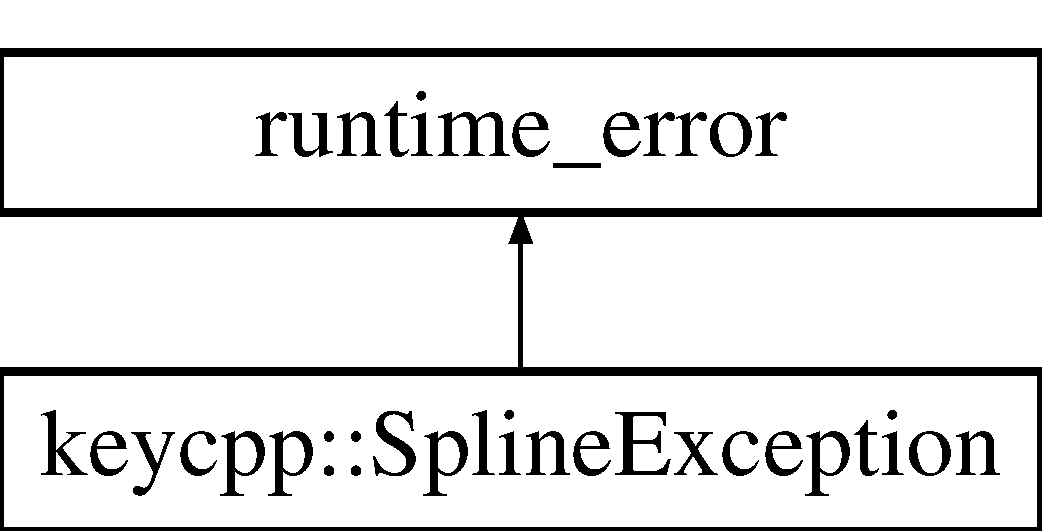
\includegraphics[height=2.000000cm]{classkeycpp_1_1_spline_exception}
\end{center}
\end{figure}
\subsection*{Public Member Functions}
\begin{DoxyCompactItemize}
\item 
\hypertarget{classkeycpp_1_1_spline_exception_a7c13b157534ec469e0b735c071192df8}{{\bfseries Spline\-Exception} (const std\-::string \&msg)}\label{classkeycpp_1_1_spline_exception_a7c13b157534ec469e0b735c071192df8}

\end{DoxyCompactItemize}


The documentation for this class was generated from the following file\-:\begin{DoxyCompactItemize}
\item 
Spline.\-h\end{DoxyCompactItemize}

\hypertarget{classkeycpp_1_1_s_v_d__type}{\section{keycpp\-:\-:S\-V\-D\-\_\-type$<$ T, X $>$ Class Template Reference}
\label{classkeycpp_1_1_s_v_d__type}\index{keycpp\-::\-S\-V\-D\-\_\-type$<$ T, X $>$@{keycpp\-::\-S\-V\-D\-\_\-type$<$ T, X $>$}}
}
\subsection*{Public Attributes}
\begin{DoxyCompactItemize}
\item 
\hypertarget{classkeycpp_1_1_s_v_d__type_afcf98e82919e015758d99cee5adb65bf}{\hyperlink{classkeycpp_1_1matrix}{matrix}$<$ X $>$ {\bfseries S}}\label{classkeycpp_1_1_s_v_d__type_afcf98e82919e015758d99cee5adb65bf}

\item 
\hypertarget{classkeycpp_1_1_s_v_d__type_a31194fbf88ec1fb87f2681d0f518761d}{\hyperlink{classkeycpp_1_1matrix}{matrix}$<$ T $>$ {\bfseries U}}\label{classkeycpp_1_1_s_v_d__type_a31194fbf88ec1fb87f2681d0f518761d}

\item 
\hypertarget{classkeycpp_1_1_s_v_d__type_ad0a6e396e2548ab4762a5676ae88e4bd}{\hyperlink{classkeycpp_1_1matrix}{matrix}$<$ T $>$ {\bfseries V}}\label{classkeycpp_1_1_s_v_d__type_ad0a6e396e2548ab4762a5676ae88e4bd}

\end{DoxyCompactItemize}


The documentation for this class was generated from the following file\-:\begin{DoxyCompactItemize}
\item 
\hyperlink{keycpp_8h}{keycpp.\-h}\end{DoxyCompactItemize}

\hypertarget{structkeycpp_1_1tictoc__type}{\section{keycpp\-:\-:tictoc\-\_\-type Struct Reference}
\label{structkeycpp_1_1tictoc__type}\index{keycpp\-::tictoc\-\_\-type@{keycpp\-::tictoc\-\_\-type}}
}


Data type for using the \hyperlink{namespacekeycpp_a6069a9eec0edfa1d401230013d98765e}{tic()} and toc(tictoc\-\_\-type Timer) commands.  




{\ttfamily \#include $<$keycpp.\-h$>$}

\subsection*{Public Attributes}
\begin{DoxyCompactItemize}
\item 
\hypertarget{structkeycpp_1_1tictoc__type_ad6878570bb9710bf65574d2296ebd287}{timeval {\bfseries start}}\label{structkeycpp_1_1tictoc__type_ad6878570bb9710bf65574d2296ebd287}

\item 
\hypertarget{structkeycpp_1_1tictoc__type_a4d57057ccd64987a00d47be2eeda40a5}{timeval {\bfseries stop}}\label{structkeycpp_1_1tictoc__type_a4d57057ccd64987a00d47be2eeda40a5}

\item 
\hypertarget{structkeycpp_1_1tictoc__type_aceaa45496add0b4c6714ac69e98c2580}{timeval {\bfseries elapsed}}\label{structkeycpp_1_1tictoc__type_aceaa45496add0b4c6714ac69e98c2580}

\end{DoxyCompactItemize}


The documentation for this struct was generated from the following file\-:\begin{DoxyCompactItemize}
\item 
\hyperlink{keycpp_8h}{keycpp.\-h}\end{DoxyCompactItemize}

\hypertarget{classkeycpp_1_1vector__k}{\section{keycpp\-:\-:vector\-\_\-k$<$ T $>$ Class Template Reference}
\label{classkeycpp_1_1vector__k}\index{keycpp\-::vector\-\_\-k$<$ T $>$@{keycpp\-::vector\-\_\-k$<$ T $>$}}
}
\subsection*{Public Types}
\begin{DoxyCompactItemize}
\item 
\hypertarget{classkeycpp_1_1vector__k_af4ac972a753299ebb2c099ed11de6382}{typedef T $\ast$ {\bfseries iterator}}\label{classkeycpp_1_1vector__k_af4ac972a753299ebb2c099ed11de6382}

\item 
\hypertarget{classkeycpp_1_1vector__k_a30a91c02d08abdf62f193f35814858c5}{typedef const T $\ast$ {\bfseries const\-\_\-iterator}}\label{classkeycpp_1_1vector__k_a30a91c02d08abdf62f193f35814858c5}

\item 
\hypertarget{classkeycpp_1_1vector__k_a66a8ed8296d754341cedd8b242fc980a}{typedef size\-\_\-t {\bfseries size\-\_\-type}}\label{classkeycpp_1_1vector__k_a66a8ed8296d754341cedd8b242fc980a}

\end{DoxyCompactItemize}
\subsection*{Public Member Functions}
\begin{DoxyCompactItemize}
\item 
\hypertarget{classkeycpp_1_1vector__k_a2fa975294c1ae939afa67863d3b84fc0}{{\bfseries vector\-\_\-k} (size\-\_\-t size)}\label{classkeycpp_1_1vector__k_a2fa975294c1ae939afa67863d3b84fc0}

\item 
\hypertarget{classkeycpp_1_1vector__k_a1f65dfce13d605312c497195081b71fa}{{\bfseries vector\-\_\-k} (size\-\_\-t size, const T \&initial)}\label{classkeycpp_1_1vector__k_a1f65dfce13d605312c497195081b71fa}

\item 
\hypertarget{classkeycpp_1_1vector__k_a6902434fbd3b5ebbbedc1b068c3df3ec}{{\bfseries vector\-\_\-k} (T $\ast$ptr, size\-\_\-t size, size\-\_\-t pinc)}\label{classkeycpp_1_1vector__k_a6902434fbd3b5ebbbedc1b068c3df3ec}

\item 
\hypertarget{classkeycpp_1_1vector__k_a5b6df14409684df91f883c3bb33204f5}{{\bfseries vector\-\_\-k} (const std\-::initializer\-\_\-list$<$ T $>$ \&lst)}\label{classkeycpp_1_1vector__k_a5b6df14409684df91f883c3bb33204f5}

\item 
\hypertarget{classkeycpp_1_1vector__k_a694c6c797022382b57e2d51350e39afc}{{\bfseries vector\-\_\-k} (const \hyperlink{classkeycpp_1_1vector__k}{vector\-\_\-k}$<$ T $>$ \&v)}\label{classkeycpp_1_1vector__k_a694c6c797022382b57e2d51350e39afc}

\item 
\hypertarget{classkeycpp_1_1vector__k_a5e130370253f66d9968c35d41228bef4}{{\bfseries vector\-\_\-k} (const std\-::vector$<$ T $>$ \&v)}\label{classkeycpp_1_1vector__k_a5e130370253f66d9968c35d41228bef4}

\item 
\hypertarget{classkeycpp_1_1vector__k_a651efbae7ea28e3e4cc3a07375a8de72}{size\-\_\-t {\bfseries capacity} () const }\label{classkeycpp_1_1vector__k_a651efbae7ea28e3e4cc3a07375a8de72}

\item 
\hypertarget{classkeycpp_1_1vector__k_a829c7caf8f696e161375d18b715c918a}{size\-\_\-t {\bfseries size} () const }\label{classkeycpp_1_1vector__k_a829c7caf8f696e161375d18b715c918a}

\item 
\hypertarget{classkeycpp_1_1vector__k_abbba6e3a7e0dc425a78645f78417c62c}{bool {\bfseries empty} () const }\label{classkeycpp_1_1vector__k_abbba6e3a7e0dc425a78645f78417c62c}

\item 
\hypertarget{classkeycpp_1_1vector__k_a57ec9796301fc1db249c531cbcb02b86}{iterator {\bfseries begin} ()}\label{classkeycpp_1_1vector__k_a57ec9796301fc1db249c531cbcb02b86}

\item 
\hypertarget{classkeycpp_1_1vector__k_ad0768d945f869ec2bae8042952ef70c3}{iterator {\bfseries end} ()}\label{classkeycpp_1_1vector__k_ad0768d945f869ec2bae8042952ef70c3}

\item 
\hypertarget{classkeycpp_1_1vector__k_a4a0b078263c4dee69535701358c62b4a}{const\-\_\-iterator {\bfseries begin} () const }\label{classkeycpp_1_1vector__k_a4a0b078263c4dee69535701358c62b4a}

\item 
\hypertarget{classkeycpp_1_1vector__k_a9453d606e3e95d4fa81e9287fc3914d3}{const\-\_\-iterator {\bfseries end} () const }\label{classkeycpp_1_1vector__k_a9453d606e3e95d4fa81e9287fc3914d3}

\item 
\hypertarget{classkeycpp_1_1vector__k_ac59a48a400d54bc34eb3355a0692a2f8}{T \& {\bfseries front} ()}\label{classkeycpp_1_1vector__k_ac59a48a400d54bc34eb3355a0692a2f8}

\item 
\hypertarget{classkeycpp_1_1vector__k_a07dff703d64e581533d2e5513a609577}{T \& {\bfseries back} ()}\label{classkeycpp_1_1vector__k_a07dff703d64e581533d2e5513a609577}

\item 
\hypertarget{classkeycpp_1_1vector__k_a3672772db9bc7c4190c3b9c10b2d8e22}{void {\bfseries push\-\_\-back} (const T \&value)}\label{classkeycpp_1_1vector__k_a3672772db9bc7c4190c3b9c10b2d8e22}

\item 
\hypertarget{classkeycpp_1_1vector__k_a3194498720cf8e14d33af58b82c70634}{void {\bfseries pop\-\_\-back} ()}\label{classkeycpp_1_1vector__k_a3194498720cf8e14d33af58b82c70634}

\item 
\hypertarget{classkeycpp_1_1vector__k_aecd33f4505867fed1e49dbe3f9470117}{void {\bfseries reserve} (size\-\_\-t capacity)}\label{classkeycpp_1_1vector__k_aecd33f4505867fed1e49dbe3f9470117}

\item 
\hypertarget{classkeycpp_1_1vector__k_a024e493fa716327aa16b2ba59771fce1}{void {\bfseries resize} (size\-\_\-t size)}\label{classkeycpp_1_1vector__k_a024e493fa716327aa16b2ba59771fce1}

\item 
\hypertarget{classkeycpp_1_1vector__k_aa7bae542df2d3ceeab63ab137a52df94}{T \& {\bfseries operator\mbox{[}$\,$\mbox{]}} (const size\-\_\-t index)}\label{classkeycpp_1_1vector__k_aa7bae542df2d3ceeab63ab137a52df94}

\item 
\hypertarget{classkeycpp_1_1vector__k_af9fc299b3eecce09bb7166954acf7b16}{const T \& {\bfseries operator\mbox{[}$\,$\mbox{]}} (const size\-\_\-t index) const }\label{classkeycpp_1_1vector__k_af9fc299b3eecce09bb7166954acf7b16}

\item 
\hypertarget{classkeycpp_1_1vector__k_ab2030403334539d7df1001e8b9037fa9}{\hyperlink{classkeycpp_1_1vector__k}{vector\-\_\-k}$<$ T $>$ \& {\bfseries operator=} (const \hyperlink{classkeycpp_1_1vector__k}{vector\-\_\-k}$<$ T $>$ \&v)}\label{classkeycpp_1_1vector__k_ab2030403334539d7df1001e8b9037fa9}

\item 
\hypertarget{classkeycpp_1_1vector__k_a318832966719bc35aa0147ec2aeabb6f}{\hyperlink{classkeycpp_1_1vector__k}{vector\-\_\-k}$<$ T $>$ \& {\bfseries operator=} (const std\-::vector$<$ T $>$ \&v)}\label{classkeycpp_1_1vector__k_a318832966719bc35aa0147ec2aeabb6f}

\item 
\hypertarget{classkeycpp_1_1vector__k_a926f7d20093e3b36e92f10aaeea1e909}{void {\bfseries clear} ()}\label{classkeycpp_1_1vector__k_a926f7d20093e3b36e92f10aaeea1e909}

\item 
\hypertarget{classkeycpp_1_1vector__k_a54ffbb92ed1926e6066d26db886b4132}{{\bfseries operator std\-::vector$<$ T $>$} ()}\label{classkeycpp_1_1vector__k_a54ffbb92ed1926e6066d26db886b4132}

\end{DoxyCompactItemize}


The documentation for this class was generated from the following file\-:\begin{DoxyCompactItemize}
\item 
vector\-\_\-k.\-h\end{DoxyCompactItemize}

\chapter{File Documentation}
\hypertarget{keycpp_8h}{\section{keycpp.\-h File Reference}
\label{keycpp_8h}\index{keycpp.\-h@{keycpp.\-h}}
}
{\ttfamily \#include $<$iostream$>$}\\*
{\ttfamily \#include $<$iomanip$>$}\\*
{\ttfamily \#include $<$complex$>$}\\*
{\ttfamily \#include $<$vector$>$}\\*
{\ttfamily \#include $<$string$>$}\\*
{\ttfamily \#include $<$cmath$>$}\\*
{\ttfamily \#include $<$boost/numeric/odeint.\-hpp$>$}\\*
{\ttfamily \#include $<$utility$>$}\\*
{\ttfamily \#include $<$algorithm$>$}\\*
{\ttfamily \#include $<$limits$>$}\\*
{\ttfamily \#include $<$ctime$>$}\\*
{\ttfamily \#include $<$stdarg.\-h$>$}\\*
{\ttfamily \#include \char`\"{}vector\-\_\-k.\-h\char`\"{}}\\*
{\ttfamily \#include \char`\"{}Matrix.\-h\char`\"{}}\\*
{\ttfamily \#include \char`\"{}kiss\-\_\-fft.\-h\char`\"{}}\\*
{\ttfamily \#include \char`\"{}Spline.\-h\char`\"{}}\\*
{\ttfamily \#include \char`\"{}Figure.\-h\char`\"{}}\\*
\subsection*{Classes}
\begin{DoxyCompactItemize}
\item 
class \hyperlink{classkeycpp_1_1_key_cpp_exception}{keycpp\-::\-Key\-Cpp\-Exception}
\item 
struct \hyperlink{structkeycpp_1_1observe}{keycpp\-::observe$<$ T, U $>$}
\item 
struct \hyperlink{structboost_1_1numeric_1_1odeint_1_1is__resizeable_3_01keycpp_1_1vector__k_3_01_t_01_4_01_4}{boost\-::numeric\-::odeint\-::is\-\_\-resizeable$<$ keycpp\-::vector\-\_\-k$<$ T $>$ $>$}
\item 
struct \hyperlink{structkeycpp_1_1_o_d_e__type}{keycpp\-::\-O\-D\-E\-\_\-type$<$ T, Y $>$}
\item 
struct \hyperlink{structkeycpp_1_1_sort___matrix}{keycpp\-::\-Sort\-\_\-\-Matrix$<$ T $>$}
\item 
struct \hyperlink{structkeycpp_1_1_sort___vector}{keycpp\-::\-Sort\-\_\-\-Vector$<$ T $>$}
\item 
struct \hyperlink{structkeycpp_1_1matrix__find__type}{keycpp\-::matrix\-\_\-find\-\_\-type$<$ T $>$}
\item 
class \hyperlink{classkeycpp_1_1_s_v_d__type}{keycpp\-::\-S\-V\-D\-\_\-type$<$ T, X $>$}
\item 
struct \hyperlink{structkeycpp_1_1tictoc__type}{keycpp\-::tictoc\-\_\-type}
\begin{DoxyCompactList}\small\item\em Data type for using the \hyperlink{namespacekeycpp_a6069a9eec0edfa1d401230013d98765e}{tic()} and toc(tictoc\-\_\-type Timer) commands. \end{DoxyCompactList}\end{DoxyCompactItemize}
\subsection*{Namespaces}
\begin{DoxyCompactItemize}
\item 
namespace \hyperlink{namespacekeycpp}{keycpp}
\begin{DoxyCompactList}\small\item\em The keycpp namespace prevents Key\-Cpp functions and classes from interfering with other C++ libraries, for instance the std library. \end{DoxyCompactList}\end{DoxyCompactItemize}
\subsection*{Functions}
\begin{DoxyCompactItemize}
\item 
\hypertarget{namespacekeycpp_a55e50932cc54f92bdd7e38c6438f4f1f}{double \hyperlink{namespacekeycpp_a55e50932cc54f92bdd7e38c6438f4f1f}{keycpp\-::ddot\-\_\-} (const int $\ast$N, const double $\ast$a, const int $\ast$inca, const double $\ast$b, const int $\ast$incb)}\label{namespacekeycpp_a55e50932cc54f92bdd7e38c6438f4f1f}

\begin{DoxyCompactList}\small\item\em This provides a C interface to B\-L\-A\-S's double dot product function. \end{DoxyCompactList}\item 
\hypertarget{namespacekeycpp_a2ce99b4fe4a13b9c70ada81761eb0ca2}{void \hyperlink{namespacekeycpp_a2ce99b4fe4a13b9c70ada81761eb0ca2}{keycpp\-::zdotu\-\_\-} (std\-::complex$<$ double $>$ $\ast$result, const int $\ast$N, const std\-::complex$<$ double $>$ $\ast$a, const int $\ast$inca, const std\-::complex$<$ double $>$ $\ast$b, const int $\ast$incb)}\label{namespacekeycpp_a2ce99b4fe4a13b9c70ada81761eb0ca2}

\begin{DoxyCompactList}\small\item\em This provides a C interface to B\-L\-A\-S's complex double dot product function. \end{DoxyCompactList}\item 
\hypertarget{namespacekeycpp_ae99c5b242a21ba683701ccb6ab6534b1}{void \hyperlink{namespacekeycpp_ae99c5b242a21ba683701ccb6ab6534b1}{keycpp\-::daxpy\-\_\-} (const int $\ast$N, const double $\ast$alpha, const double $\ast$x, const int $\ast$incx, double $\ast$y, const int $\ast$incy)}\label{namespacekeycpp_ae99c5b242a21ba683701ccb6ab6534b1}

\begin{DoxyCompactList}\small\item\em This provides a C interface to B\-L\-A\-S's double vector addition function. \end{DoxyCompactList}\item 
\hypertarget{namespacekeycpp_a6460fa334239dde761d8f737b9438fed}{void \hyperlink{namespacekeycpp_a6460fa334239dde761d8f737b9438fed}{keycpp\-::zaxpy\-\_\-} (const int $\ast$N, const std\-::complex$<$ double $>$ $\ast$alpha, const std\-::complex$<$ double $>$ $\ast$x, const int $\ast$incx, std\-::complex$<$ double $>$ $\ast$y, const int $\ast$incy)}\label{namespacekeycpp_a6460fa334239dde761d8f737b9438fed}

\begin{DoxyCompactList}\small\item\em This provides a C interface to B\-L\-A\-S's complex double vector addition function. \end{DoxyCompactList}\item 
\hypertarget{namespacekeycpp_a7d249dd978770119c1b91d88009fefbd}{void \hyperlink{namespacekeycpp_a7d249dd978770119c1b91d88009fefbd}{keycpp\-::dscal\-\_\-} (const int $\ast$N, const double $\ast$alpha, double $\ast$x, const int $\ast$incx)}\label{namespacekeycpp_a7d249dd978770119c1b91d88009fefbd}

\begin{DoxyCompactList}\small\item\em This provides a C interface to B\-L\-A\-S's double scalar-\/vector multiplication function. \end{DoxyCompactList}\item 
\hypertarget{namespacekeycpp_ad9dd69d0d355e4805a832813199f1dff}{void \hyperlink{namespacekeycpp_ad9dd69d0d355e4805a832813199f1dff}{keycpp\-::zscal\-\_\-} (const int $\ast$N, const std\-::complex$<$ double $>$ $\ast$alpha, std\-::complex$<$ double $>$ $\ast$x, const int $\ast$incx)}\label{namespacekeycpp_ad9dd69d0d355e4805a832813199f1dff}

\begin{DoxyCompactList}\small\item\em This provides a C interface to B\-L\-A\-S's complex double scalar-\/vector multiplication function. \end{DoxyCompactList}\item 
\hypertarget{namespacekeycpp_ace2501951ab3db3a91c3520ae89750b1}{void \hyperlink{namespacekeycpp_ace2501951ab3db3a91c3520ae89750b1}{keycpp\-::zggev\-\_\-} (const char $\ast$jobvl, const char $\ast$jobvr, const int $\ast$n, std\-::complex$<$ double $>$ $\ast$a, const int $\ast$lda, std\-::complex$<$ double $>$ $\ast$b, const int $\ast$ldb, std\-::complex$<$ double $>$ $\ast$alpha, std\-::complex$<$ double $>$ $\ast$beta, std\-::complex$<$ double $>$ $\ast$vl, const int $\ast$ldvl, std\-::complex$<$ double $>$ $\ast$vr, const int $\ast$ldvr, std\-::complex$<$ double $>$ $\ast$work, const int $\ast$lwork, double $\ast$rwork, int $\ast$info)}\label{namespacekeycpp_ace2501951ab3db3a91c3520ae89750b1}

\begin{DoxyCompactList}\small\item\em This provides a C interface to L\-A\-P\-A\-C\-K's complex generalized eigenvalue solver. \end{DoxyCompactList}\item 
\hypertarget{namespacekeycpp_aebc5253e80ac15a9bfdc5449ae4f972a}{void \hyperlink{namespacekeycpp_aebc5253e80ac15a9bfdc5449ae4f972a}{keycpp\-::dgeev\-\_\-} (const char $\ast$jobvl, const char $\ast$jobvr, const int $\ast$n, double $\ast$A, const int $\ast$lda, double $\ast$wr, double $\ast$wi, double $\ast$vl, const int $\ast$ldvl, double $\ast$vr, const int $\ast$ldvr, double $\ast$work, const int $\ast$lwork, int $\ast$info)}\label{namespacekeycpp_aebc5253e80ac15a9bfdc5449ae4f972a}

\begin{DoxyCompactList}\small\item\em This provides a C interface to L\-A\-P\-A\-C\-K's double precision eigenvalue solver for a general matrix. \end{DoxyCompactList}\item 
\hypertarget{namespacekeycpp_a8c1cca2a162f40fc6c6218c35cadf9f2}{void \hyperlink{namespacekeycpp_a8c1cca2a162f40fc6c6218c35cadf9f2}{keycpp\-::zgeev\-\_\-} (const char $\ast$jobvl, const char $\ast$, const int $\ast$n, std\-::complex$<$ double $>$ $\ast$A, const int $\ast$lda, std\-::complex$<$ double $>$ $\ast$w, std\-::complex$<$ double $>$ $\ast$V\-L, const int $\ast$ldvl, std\-::complex$<$ double $>$ $\ast$V\-R, const int $\ast$ldvr, std\-::complex$<$ double $>$ $\ast$work, const int $\ast$lwork, double $\ast$rwork, int $\ast$info)}\label{namespacekeycpp_a8c1cca2a162f40fc6c6218c35cadf9f2}

\begin{DoxyCompactList}\small\item\em This provides a C interface to L\-A\-P\-A\-C\-K's complex eigenvalue solver for a general matrix. \end{DoxyCompactList}\item 
\hypertarget{namespacekeycpp_aca3be6524e195662cbb74a810305e721}{void \hyperlink{namespacekeycpp_aca3be6524e195662cbb74a810305e721}{keycpp\-::dgecon\-\_\-} (const char $\ast$norm, const int $\ast$n, double $\ast$a, const int $\ast$lda, const double $\ast$anorm, double $\ast$rcond, double $\ast$work, int $\ast$iwork, int $\ast$info)}\label{namespacekeycpp_aca3be6524e195662cbb74a810305e721}

\begin{DoxyCompactList}\small\item\em This provides a C interface to L\-A\-P\-A\-C\-K's double precision reciprocal condition number estimator. \end{DoxyCompactList}\item 
\hypertarget{namespacekeycpp_a75e334ffaf1864d7191e9e0b64189783}{void \hyperlink{namespacekeycpp_a75e334ffaf1864d7191e9e0b64189783}{keycpp\-::dgetrf\-\_\-} (const int $\ast$m, const int $\ast$n, double $\ast$a, const int $\ast$lda, int $\ast$lpiv, int $\ast$info)}\label{namespacekeycpp_a75e334ffaf1864d7191e9e0b64189783}

\begin{DoxyCompactList}\small\item\em This provides a C interface to L\-A\-P\-A\-C\-K's double precision L\-U decomposition function. \end{DoxyCompactList}\item 
\hypertarget{namespacekeycpp_ab9c33788a2c083aa5738eda1fe62a261}{void \hyperlink{namespacekeycpp_ab9c33788a2c083aa5738eda1fe62a261}{keycpp\-::dgetrs\-\_\-} (const char $\ast$trans, int $\ast$n, int $\ast$nrhs, double $\ast$a, const int $\ast$lda, int $\ast$ipiv, double $\ast$b, int $\ast$ldb, int $\ast$info)}\label{namespacekeycpp_ab9c33788a2c083aa5738eda1fe62a261}

\begin{DoxyCompactList}\small\item\em This provides a C interface to L\-A\-P\-A\-C\-K's double precision L\-U solver. \end{DoxyCompactList}\item 
\hypertarget{namespacekeycpp_a4507ef954be960fec70ca0f93258d730}{double \hyperlink{namespacekeycpp_a4507ef954be960fec70ca0f93258d730}{keycpp\-::dlange\-\_\-} (const char $\ast$norm, const int $\ast$m, const int $\ast$n, const double $\ast$a, const int $\ast$lda, double $\ast$work)}\label{namespacekeycpp_a4507ef954be960fec70ca0f93258d730}

\begin{DoxyCompactList}\small\item\em This provides a C interface to L\-A\-P\-A\-C\-K's double precision norm function. \end{DoxyCompactList}\item 
\hypertarget{namespacekeycpp_a444e3cdc7e7929414370b6b50ea1218c}{void \hyperlink{namespacekeycpp_a444e3cdc7e7929414370b6b50ea1218c}{keycpp\-::zgecon\-\_\-} (const char $\ast$norm, const int $\ast$n, std\-::complex$<$ double $>$ $\ast$a, const int $\ast$lda, const double $\ast$anorm, double $\ast$rcond, std\-::complex$<$ double $>$ $\ast$work, double $\ast$rwork, int $\ast$info)}\label{namespacekeycpp_a444e3cdc7e7929414370b6b50ea1218c}

\begin{DoxyCompactList}\small\item\em This provides a C interface to L\-A\-P\-A\-C\-K's complex-\/valued reciprocal condition number estimator. \end{DoxyCompactList}\item 
\hypertarget{namespacekeycpp_ab18d58d53d8e19a37d74d24da27a64dd}{void \hyperlink{namespacekeycpp_ab18d58d53d8e19a37d74d24da27a64dd}{keycpp\-::zgetrf\-\_\-} (const int $\ast$m, const int $\ast$n, std\-::complex$<$ double $>$ $\ast$a, const int $\ast$lda, int $\ast$lpiv, int $\ast$info)}\label{namespacekeycpp_ab18d58d53d8e19a37d74d24da27a64dd}

\begin{DoxyCompactList}\small\item\em This provides a C interface to L\-A\-P\-A\-C\-K's complex L\-U decomposition function. \end{DoxyCompactList}\item 
\hypertarget{namespacekeycpp_abbe4322276dcdb7d864e85854b5b90f2}{void \hyperlink{namespacekeycpp_abbe4322276dcdb7d864e85854b5b90f2}{keycpp\-::zgetrs\-\_\-} (const char $\ast$trans, int $\ast$n, int $\ast$nrhs, std\-::complex$<$ double $>$ $\ast$a, const int $\ast$lda, int $\ast$ipiv, std\-::complex$<$ double $>$ $\ast$b, int $\ast$ldb, int $\ast$info)}\label{namespacekeycpp_abbe4322276dcdb7d864e85854b5b90f2}

\begin{DoxyCompactList}\small\item\em This provides a C interface to L\-A\-P\-A\-C\-K's complex L\-U solver. \end{DoxyCompactList}\item 
\hypertarget{namespacekeycpp_a1477c910b07baef984fe8528c29b2774}{double \hyperlink{namespacekeycpp_a1477c910b07baef984fe8528c29b2774}{keycpp\-::zlange\-\_\-} (const char $\ast$norm, const int $\ast$m, const int $\ast$n, const std\-::complex$<$ double $>$ $\ast$a, const int $\ast$lda, double $\ast$work)}\label{namespacekeycpp_a1477c910b07baef984fe8528c29b2774}

\begin{DoxyCompactList}\small\item\em This provides a C interface to L\-A\-P\-A\-C\-K's complex norm function. \end{DoxyCompactList}\item 
\hypertarget{namespacekeycpp_a12719f4b48de048f9642066666a920bd}{void \hyperlink{namespacekeycpp_a12719f4b48de048f9642066666a920bd}{keycpp\-::dgesv\-\_\-} (const int $\ast$n, const int $\ast$nrhs, double $\ast$a, const int $\ast$lda, int $\ast$ipiv, double $\ast$b, const int $\ast$ldb, const int $\ast$info)}\label{namespacekeycpp_a12719f4b48de048f9642066666a920bd}

\begin{DoxyCompactList}\small\item\em This provides a C interface to L\-A\-P\-A\-C\-K's double precision linear system solver. \end{DoxyCompactList}\item 
\hypertarget{namespacekeycpp_af92d0d887ae48cc4222f7167232a7f82}{void \hyperlink{namespacekeycpp_af92d0d887ae48cc4222f7167232a7f82}{keycpp\-::dgetri\-\_\-} (const int $\ast$n, double $\ast$A, const int $\ast$lda, const int $\ast$ipiv, double $\ast$work, const int $\ast$lwork, int $\ast$info)}\label{namespacekeycpp_af92d0d887ae48cc4222f7167232a7f82}

\begin{DoxyCompactList}\small\item\em This provides a C interface to L\-A\-P\-A\-C\-K's double precision matrix inverse function. \end{DoxyCompactList}\item 
\hypertarget{namespacekeycpp_a4190e125fe33133aafa586089ca6e174}{void \hyperlink{namespacekeycpp_a4190e125fe33133aafa586089ca6e174}{keycpp\-::zgetri\-\_\-} (const int $\ast$n, std\-::complex$<$ double $>$ $\ast$A, const int $\ast$lda, const int $\ast$ipiv, std\-::complex$<$ double $>$ $\ast$work, const int $\ast$lwork, int $\ast$info)}\label{namespacekeycpp_a4190e125fe33133aafa586089ca6e174}

\begin{DoxyCompactList}\small\item\em This provides a C interface to L\-A\-P\-A\-C\-K's complex matrix inverse function. \end{DoxyCompactList}\item 
\hypertarget{namespacekeycpp_a8fe7a71afbb6c5dc049cdd7afff6c0af}{void \hyperlink{namespacekeycpp_a8fe7a71afbb6c5dc049cdd7afff6c0af}{keycpp\-::dgesvd\-\_\-} (const char $\ast$jobu, const char $\ast$jobvt, const int $\ast$m, const int $\ast$n, double $\ast$A, const int $\ast$lda, double $\ast$S, double $\ast$U, const int $\ast$ldu, double $\ast$V\-T, const int $\ast$ldvt, double $\ast$work, const int $\ast$lwork, int $\ast$info)}\label{namespacekeycpp_a8fe7a71afbb6c5dc049cdd7afff6c0af}

\begin{DoxyCompactList}\small\item\em This provides a C interface to L\-A\-P\-A\-C\-K's double precision S\-V\-D function. \end{DoxyCompactList}\item 
\hypertarget{namespacekeycpp_afa5e2f74110f53bd288c15ce1f183f9b}{void \hyperlink{namespacekeycpp_afa5e2f74110f53bd288c15ce1f183f9b}{keycpp\-::zgesvd\-\_\-} (const char $\ast$jobu, const char $\ast$jobvt, const int $\ast$m, const int $\ast$n, std\-::complex$<$ double $>$ $\ast$A, const int $\ast$lda, double $\ast$S, std\-::complex$<$ double $>$ $\ast$U, const int $\ast$ldu, std\-::complex$<$ double $>$ $\ast$V\-T, const int $\ast$ldvt, std\-::complex$<$ double $>$ $\ast$work, const int $\ast$lwork, double $\ast$rwork, int $\ast$info)}\label{namespacekeycpp_afa5e2f74110f53bd288c15ce1f183f9b}

\begin{DoxyCompactList}\small\item\em This provides a C interface to L\-A\-P\-A\-C\-K's complex S\-V\-D function. \end{DoxyCompactList}\item 
\hypertarget{namespacekeycpp_ab08546b5ffdc4b792b2a835c823340cc}{vector\-\_\-k$<$ std\-::complex$<$ double $>$ $>$ {\bfseries keycpp\-::eig} (const matrix$<$ std\-::complex$<$ double $>$ $>$ \&A, const matrix$<$ std\-::complex$<$ double $>$ $>$ \&B, matrix$<$ std\-::complex$<$ double $>$ $>$ $\ast$vr\-\_\-return=N\-U\-L\-L, matrix$<$ std\-::complex$<$ double $>$ $>$ $\ast$vl\-\_\-return=N\-U\-L\-L)}\label{namespacekeycpp_ab08546b5ffdc4b792b2a835c823340cc}

\item 
\hypertarget{namespacekeycpp_a192bcf724ea788d3d3e759117220e940}{vector\-\_\-k$<$ std\-::complex$<$ double $>$ $>$ {\bfseries keycpp\-::eig} (const matrix$<$ std\-::complex$<$ double $>$ $>$ \&A, matrix$<$ std\-::complex$<$ double $>$ $>$ $\ast$vr\-\_\-return=N\-U\-L\-L, matrix$<$ std\-::complex$<$ double $>$ $>$ $\ast$vl\-\_\-return=N\-U\-L\-L)}\label{namespacekeycpp_a192bcf724ea788d3d3e759117220e940}

\item 
\hypertarget{namespacekeycpp_a42950497e518f5882a0689bb78fa667f}{vector\-\_\-k$<$ std\-::complex$<$ double $>$ $>$ {\bfseries keycpp\-::eig} (const matrix$<$ double $>$ \&A, matrix$<$ std\-::complex$<$ double $>$$>$ $\ast$vr\-\_\-return=N\-U\-L\-L, matrix$<$ std\-::complex$<$ double $>$$>$ $\ast$vl\-\_\-return=N\-U\-L\-L)}\label{namespacekeycpp_a42950497e518f5882a0689bb78fa667f}

\item 
\hypertarget{namespacekeycpp_a3905cfc35dbd146f5dbf7bcb5729c2c2}{double {\bfseries keycpp\-::rcond} (const matrix$<$ double $>$ \&A)}\label{namespacekeycpp_a3905cfc35dbd146f5dbf7bcb5729c2c2}

\item 
\hypertarget{namespacekeycpp_a4d9a9dd04453e5a417f7a9eb8ae4391b}{double {\bfseries keycpp\-::rcond} (const matrix$<$ std\-::complex$<$ double $>$$>$ \&A)}\label{namespacekeycpp_a4d9a9dd04453e5a417f7a9eb8ae4391b}

\item 
\hypertarget{namespacekeycpp_ad650072c8cf30a8674431dcf414b1c3b}{vector\-\_\-k$<$ std\-::complex$<$ double $>$ $>$ {\bfseries keycpp\-::linsolve} (const matrix$<$ std\-::complex$<$ double $>$$>$ \&A\-\_\-in, const vector\-\_\-k$<$ std\-::complex$<$ double $>$$>$ \&b\-\_\-in)}\label{namespacekeycpp_ad650072c8cf30a8674431dcf414b1c3b}

\item 
\hypertarget{namespacekeycpp_a13a89a2c6d30c991f4de63ca8f62c0e1}{vector\-\_\-k$<$ double $>$ {\bfseries keycpp\-::linsolve} (const matrix$<$ double $>$ \&A\-\_\-in, const vector\-\_\-k$<$ double $>$ \&b\-\_\-in)}\label{namespacekeycpp_a13a89a2c6d30c991f4de63ca8f62c0e1}

\item 
\hypertarget{namespacekeycpp_adc96927cda2df7a6e8e2031941c43601}{matrix$<$ double $>$ {\bfseries keycpp\-::inv} (const matrix$<$ double $>$ \&A\-\_\-in)}\label{namespacekeycpp_adc96927cda2df7a6e8e2031941c43601}

\item 
\hypertarget{namespacekeycpp_a6b74369f5415c3ed45f63995149ad992}{matrix$<$ std\-::complex$<$ double $>$ $>$ {\bfseries keycpp\-::inv} (const matrix$<$ std\-::complex$<$ double $>$$>$ \&A\-\_\-in)}\label{namespacekeycpp_a6b74369f5415c3ed45f63995149ad992}

\item 
\hypertarget{namespacekeycpp_a5ef5c1f5951e8182a7c4ec9612f3f7e1}{double \hyperlink{namespacekeycpp_a5ef5c1f5951e8182a7c4ec9612f3f7e1}{keycpp\-::rand} ()}\label{namespacekeycpp_a5ef5c1f5951e8182a7c4ec9612f3f7e1}

\begin{DoxyCompactList}\small\item\em Returns a random double between 0 and 1.\-0. \end{DoxyCompactList}\item 
\hypertarget{namespacekeycpp_ac224964eb5e1a55c3f7d58f0e9b71d3d}{matrix$<$ double $>$ {\bfseries keycpp\-::rand} (const int \&N)}\label{namespacekeycpp_ac224964eb5e1a55c3f7d58f0e9b71d3d}

\item 
\hypertarget{namespacekeycpp_ae5c4b142a4101e9bb1df9f19efaf7d2f}{matrix$<$ double $>$ {\bfseries keycpp\-::rand} (const int \&M, const int \&N)}\label{namespacekeycpp_ae5c4b142a4101e9bb1df9f19efaf7d2f}

\item 
\hypertarget{namespacekeycpp_aae90693acdaf666bd23bf861f2c0d28c}{{\footnotesize template$<$class T $>$ }\\matrix$<$ T $>$ {\bfseries keycpp\-::eop} (const matrix$<$ T $>$ \&A, T($\ast$f)(const T \&))}\label{namespacekeycpp_aae90693acdaf666bd23bf861f2c0d28c}

\item 
\hypertarget{namespacekeycpp_a6c6542964c7aaaccbee336567f64c03c}{{\footnotesize template$<$class T $>$ }\\vector\-\_\-k$<$ T $>$ {\bfseries keycpp\-::eop} (const vector\-\_\-k$<$ T $>$ \&v1, T($\ast$f)(const T \&))}\label{namespacekeycpp_a6c6542964c7aaaccbee336567f64c03c}

\item 
\hypertarget{namespacekeycpp_a3a1ba458353cfecef659b40e446baaf0}{{\footnotesize template$<$class T $>$ }\\matrix$<$ T $>$ {\bfseries keycpp\-::eop} (const matrix$<$ T $>$ \&A, T($\ast$f)(T))}\label{namespacekeycpp_a3a1ba458353cfecef659b40e446baaf0}

\item 
\hypertarget{namespacekeycpp_a48fb1c8a89210ed78554ecd0bed92a59}{{\footnotesize template$<$class T $>$ }\\vector\-\_\-k$<$ T $>$ {\bfseries keycpp\-::eop} (const vector\-\_\-k$<$ T $>$ \&v1, T($\ast$f)(T))}\label{namespacekeycpp_a48fb1c8a89210ed78554ecd0bed92a59}

\item 
\hypertarget{namespacekeycpp_a5afc215befa38bf47fb52cff33794ebe}{{\footnotesize template$<$class T $>$ }\\matrix$<$ T $>$ {\bfseries keycpp\-::eop} (const matrix$<$ std\-::complex$<$ T $>$$>$ \&A, T($\ast$f)(const std\-::complex$<$ T $>$ \&))}\label{namespacekeycpp_a5afc215befa38bf47fb52cff33794ebe}

\item 
\hypertarget{namespacekeycpp_afc7610588aa92335352b2796ebdd359d}{{\footnotesize template$<$class T $>$ }\\vector\-\_\-k$<$ T $>$ {\bfseries keycpp\-::eop} (const vector\-\_\-k$<$ std\-::complex$<$ T $>$$>$ \&v1, T($\ast$f)(const std\-::complex$<$ T $>$ \&))}\label{namespacekeycpp_afc7610588aa92335352b2796ebdd359d}

\item 
\hypertarget{namespacekeycpp_ae14b016d01024e738c3110299ee58666}{{\footnotesize template$<$class T $>$ }\\matrix$<$ T $>$ {\bfseries keycpp\-::eop} (const matrix$<$ std\-::complex$<$ T $>$$>$ \&A, T($\ast$f)(std\-::complex$<$ T $>$))}\label{namespacekeycpp_ae14b016d01024e738c3110299ee58666}

\item 
\hypertarget{namespacekeycpp_a31115adc10089fbbc732d59362890af2}{{\footnotesize template$<$class T $>$ }\\vector\-\_\-k$<$ T $>$ {\bfseries keycpp\-::eop} (const vector\-\_\-k$<$ std\-::complex$<$ T $>$$>$ \&v1, T($\ast$f)(std\-::complex$<$ T $>$))}\label{namespacekeycpp_a31115adc10089fbbc732d59362890af2}

\item 
\hypertarget{namespacekeycpp_a55e8bada51586c0561e1b32ca1ab5f2a}{{\footnotesize template$<$class T $>$ }\\std\-::ostream \& {\bfseries keycpp\-::operator$<$$<$} (std\-::ostream \&out, const matrix$<$ T $>$ \&A)}\label{namespacekeycpp_a55e8bada51586c0561e1b32ca1ab5f2a}

\item 
\hypertarget{namespacekeycpp_a86f8946c126102b4467b70da16766b7a}{{\footnotesize template$<$class T $>$ }\\std\-::ostream \& {\bfseries keycpp\-::operator$<$$<$} (std\-::ostream \&out, const vector\-\_\-k$<$ T $>$ \&v1)}\label{namespacekeycpp_a86f8946c126102b4467b70da16766b7a}

\item 
\hypertarget{namespacekeycpp_add55ad2a40111d6368744a3d4144f25a}{{\footnotesize template$<$class T $>$ }\\T \hyperlink{namespacekeycpp_add55ad2a40111d6368744a3d4144f25a}{keycpp\-::prod} (const vector\-\_\-k$<$ T $>$ \&x)}\label{namespacekeycpp_add55ad2a40111d6368744a3d4144f25a}

\begin{DoxyCompactList}\small\item\em Returns the product of all the elements of the vector x. \end{DoxyCompactList}\item 
\hypertarget{namespacekeycpp_af5471fc9074471701bde9e68eb7971b4}{{\footnotesize template$<$class T $>$ }\\vector\-\_\-k$<$ T $>$ \hyperlink{namespacekeycpp_af5471fc9074471701bde9e68eb7971b4}{keycpp\-::prod} (const matrix$<$ T $>$ \&A)}\label{namespacekeycpp_af5471fc9074471701bde9e68eb7971b4}

\begin{DoxyCompactList}\small\item\em Returns a vector containing the product of all the elements in each column of the matrix A. \end{DoxyCompactList}\item 
\hypertarget{namespacekeycpp_a52c37ec9c41349fd6bd862b8ebdd01bb}{{\footnotesize template$<$class T $>$ }\\vector\-\_\-k$<$ T $>$ \hyperlink{namespacekeycpp_a52c37ec9c41349fd6bd862b8ebdd01bb}{keycpp\-::diff} (const vector\-\_\-k$<$ T $>$ \&v1)}\label{namespacekeycpp_a52c37ec9c41349fd6bd862b8ebdd01bb}

\begin{DoxyCompactList}\small\item\em Returns a vector of differences between adjacent elements. \end{DoxyCompactList}\item 
{\footnotesize template$<$class T $>$ }\\matrix$<$ T $>$ \hyperlink{namespacekeycpp_abb4e57814fd30b7b8d4845bbc16c73e9}{keycpp\-::diff} (const matrix$<$ T $>$ \&A)
\begin{DoxyCompactList}\small\item\em Returns a matrix of row differences between adjacent rows. \end{DoxyCompactList}\item 
\hypertarget{namespacekeycpp_a436cfe206bb34dfe613ac495e792b155}{{\footnotesize template$<$class T $>$ }\\vector\-\_\-k$<$ std\-::complex$<$ T $>$ $>$ {\bfseries keycpp\-::conj} (const vector\-\_\-k$<$ std\-::complex$<$ T $>$$>$ \&v1)}\label{namespacekeycpp_a436cfe206bb34dfe613ac495e792b155}

\item 
\hypertarget{namespacekeycpp_a0f000b392fbefccdb089383bb6a20151}{{\footnotesize template$<$class T $>$ }\\matrix$<$ std\-::complex$<$ T $>$ $>$ {\bfseries keycpp\-::conj} (const matrix$<$ std\-::complex$<$ T $>$$>$ \&A)}\label{namespacekeycpp_a0f000b392fbefccdb089383bb6a20151}

\item 
\hypertarget{namespacekeycpp_a5b72a83172512bb554f5e443b9b366bd}{{\footnotesize template$<$class T $>$ }\\vector\-\_\-k$<$ T $>$ {\bfseries keycpp\-::real} (const vector\-\_\-k$<$ std\-::complex$<$ T $>$$>$ \&v1)}\label{namespacekeycpp_a5b72a83172512bb554f5e443b9b366bd}

\item 
\hypertarget{namespacekeycpp_a61efb014b42cd8b02a81b4520c41ab2c}{{\footnotesize template$<$class T $>$ }\\matrix$<$ T $>$ {\bfseries keycpp\-::real} (const matrix$<$ std\-::complex$<$ T $>$$>$ \&A)}\label{namespacekeycpp_a61efb014b42cd8b02a81b4520c41ab2c}

\item 
\hypertarget{namespacekeycpp_a752e14fae8ca75a5702c89207a7cd983}{{\footnotesize template$<$class T $>$ }\\vector\-\_\-k$<$ T $>$ {\bfseries keycpp\-::imag} (const vector\-\_\-k$<$ std\-::complex$<$ T $>$$>$ \&v1)}\label{namespacekeycpp_a752e14fae8ca75a5702c89207a7cd983}

\item 
\hypertarget{namespacekeycpp_ad902a14fdaa4b744a8a11220f5be0161}{{\footnotesize template$<$class T $>$ }\\matrix$<$ T $>$ {\bfseries keycpp\-::imag} (const matrix$<$ std\-::complex$<$ T $>$$>$ \&A)}\label{namespacekeycpp_ad902a14fdaa4b744a8a11220f5be0161}

\item 
\hypertarget{namespacekeycpp_a83cec179e95af014706ce54194efd1b9}{{\footnotesize template$<$class T $>$ }\\vector\-\_\-k$<$ T $>$ {\bfseries keycpp\-::abs} (const vector\-\_\-k$<$ T $>$ \&v1)}\label{namespacekeycpp_a83cec179e95af014706ce54194efd1b9}

\item 
\hypertarget{namespacekeycpp_aa48f282087263edb46886e9390b9a833}{{\footnotesize template$<$class T $>$ }\\vector\-\_\-k$<$ T $>$ {\bfseries keycpp\-::abs} (const vector\-\_\-k$<$ std\-::complex$<$ T $>$$>$ \&v1)}\label{namespacekeycpp_aa48f282087263edb46886e9390b9a833}

\item 
\hypertarget{namespacekeycpp_a1f83b48bfedf753904dfea9dde554a4c}{{\footnotesize template$<$class T $>$ }\\matrix$<$ T $>$ {\bfseries keycpp\-::abs} (const matrix$<$ T $>$ \&A)}\label{namespacekeycpp_a1f83b48bfedf753904dfea9dde554a4c}

\item 
\hypertarget{namespacekeycpp_ae0edec63f48a81c576da0c0ffc768af9}{{\footnotesize template$<$class T $>$ }\\matrix$<$ T $>$ {\bfseries keycpp\-::abs} (const matrix$<$ std\-::complex$<$ T $>$$>$ \&A)}\label{namespacekeycpp_ae0edec63f48a81c576da0c0ffc768af9}

\item 
\hypertarget{namespacekeycpp_a952e5296774667c3be4e792b5cd980da}{std\-::complex$<$ double $>$ {\bfseries keycpp\-::csqrt} (const double \&a)}\label{namespacekeycpp_a952e5296774667c3be4e792b5cd980da}

\item 
\hypertarget{namespacekeycpp_a8faa7912f1f198c5185cb6a36cfd2fb2}{std\-::complex$<$ double $>$ {\bfseries keycpp\-::csqrt} (const std\-::complex$<$ double $>$ \&a)}\label{namespacekeycpp_a8faa7912f1f198c5185cb6a36cfd2fb2}

\item 
\hypertarget{namespacekeycpp_aa865f0bd18bdefcf413b1c3dd286b998}{{\footnotesize template$<$class T , class U $>$ }\\vector\-\_\-k$<$ decltype(std\-::declval\\*
$<$ T $>$)$\ast$std\-::declval$<$ U $>$))$>$ {\bfseries keycpp\-::operator+} (const vector\-\_\-k$<$ T $>$ \&v1, const vector\-\_\-k$<$ U $>$ \&v2)}\label{namespacekeycpp_aa865f0bd18bdefcf413b1c3dd286b998}

\item 
\hypertarget{namespacekeycpp_ae416b3cc307c30afdb62f0ed37b70e05}{{\footnotesize template$<$$>$ }\\vector\-\_\-k$<$ double $>$ {\bfseries keycpp\-::operator+} (const vector\-\_\-k$<$ double $>$ \&v1, const vector\-\_\-k$<$ double $>$ \&v2)}\label{namespacekeycpp_ae416b3cc307c30afdb62f0ed37b70e05}

\item 
\hypertarget{namespacekeycpp_ade9508aa24d2496bd63dcdb72229c8b0}{{\footnotesize template$<$$>$ }\\vector\-\_\-k$<$ std\-::complex$<$ double $>$ $>$ {\bfseries keycpp\-::operator+} (const vector\-\_\-k$<$ std\-::complex$<$ double $>$$>$ \&v1, const vector\-\_\-k$<$ std\-::complex$<$ double $>$$>$ \&v2)}\label{namespacekeycpp_ade9508aa24d2496bd63dcdb72229c8b0}

\item 
\hypertarget{namespacekeycpp_a68fe0fe851bce021be6a0609da7df82d}{{\footnotesize template$<$class T , class U $>$ }\\vector\-\_\-k$<$ decltype(std\-::declval\\*
$<$ T $>$)$\ast$std\-::declval$<$ U $>$))$>$ {\bfseries keycpp\-::operator+} (const vector\-\_\-k$<$ T $>$ \&v1, const U \&a)}\label{namespacekeycpp_a68fe0fe851bce021be6a0609da7df82d}

\item 
\hypertarget{namespacekeycpp_af28312b8c309091f03e373e1ae5f3d46}{{\footnotesize template$<$class T , class U $>$ }\\vector\-\_\-k$<$ decltype(std\-::declval\\*
$<$ T $>$)$\ast$std\-::declval$<$ U $>$))$>$ {\bfseries keycpp\-::operator+} (const U \&a, const vector\-\_\-k$<$ T $>$ \&v2)}\label{namespacekeycpp_af28312b8c309091f03e373e1ae5f3d46}

\item 
\hypertarget{namespacekeycpp_adff86e062c6497110b7505b0ef715c2c}{{\footnotesize template$<$class T , class U $>$ }\\matrix$<$ decltype(std\-::declval\\*
$<$ T $>$)$\ast$std\-::declval$<$ U $>$))$>$ {\bfseries keycpp\-::operator+} (const matrix$<$ T $>$ \&A, const U \&a)}\label{namespacekeycpp_adff86e062c6497110b7505b0ef715c2c}

\item 
\hypertarget{namespacekeycpp_a4b4a64905c9d681c174b2dfcfba272c4}{{\footnotesize template$<$class T , class U $>$ }\\matrix$<$ decltype(std\-::declval\\*
$<$ T $>$)$\ast$std\-::declval$<$ U $>$))$>$ {\bfseries keycpp\-::operator+} (const U \&a, const matrix$<$ T $>$ \&A)}\label{namespacekeycpp_a4b4a64905c9d681c174b2dfcfba272c4}

\item 
\hypertarget{namespacekeycpp_a520b72efca1fbe800845b21a84d2d472}{{\footnotesize template$<$class T , class U $>$ }\\vector\-\_\-k$<$ decltype(std\-::declval\\*
$<$ T $>$)$\ast$std\-::declval$<$ U $>$))$>$ {\bfseries keycpp\-::operator-\/} (const vector\-\_\-k$<$ T $>$ \&v1, const U \&a)}\label{namespacekeycpp_a520b72efca1fbe800845b21a84d2d472}

\item 
\hypertarget{namespacekeycpp_a1222c1fe6037feb8eacf0d2bd5152751}{{\footnotesize template$<$class T , class U $>$ }\\vector\-\_\-k$<$ decltype(std\-::declval\\*
$<$ T $>$)$\ast$std\-::declval$<$ U $>$))$>$ {\bfseries keycpp\-::operator-\/} (const U \&a, const vector\-\_\-k$<$ T $>$ \&v2)}\label{namespacekeycpp_a1222c1fe6037feb8eacf0d2bd5152751}

\item 
\hypertarget{namespacekeycpp_a71a8f2ebc458f06e29b17ecc28ed000d}{{\footnotesize template$<$class T , class U $>$ }\\matrix$<$ decltype(std\-::declval\\*
$<$ T $>$)$\ast$std\-::declval$<$ U $>$))$>$ {\bfseries keycpp\-::operator-\/} (const matrix$<$ T $>$ \&A, const U \&a)}\label{namespacekeycpp_a71a8f2ebc458f06e29b17ecc28ed000d}

\item 
\hypertarget{namespacekeycpp_a4bc853f9410d964ef9f163ce53ea4828}{{\footnotesize template$<$class T , class U $>$ }\\matrix$<$ decltype(std\-::declval\\*
$<$ T $>$)$\ast$std\-::declval$<$ U $>$))$>$ {\bfseries keycpp\-::operator-\/} (const U \&a, const matrix$<$ T $>$ \&A)}\label{namespacekeycpp_a4bc853f9410d964ef9f163ce53ea4828}

\item 
\hypertarget{namespacekeycpp_a891589b60d1c968b44986f3b7d56586b}{{\footnotesize template$<$class T , class U $>$ }\\vector\-\_\-k$<$ decltype(std\-::declval\\*
$<$ T $>$)$\ast$std\-::declval$<$ U $>$))$>$ {\bfseries keycpp\-::operator-\/} (const vector\-\_\-k$<$ T $>$ \&v1, const vector\-\_\-k$<$ U $>$ \&v2)}\label{namespacekeycpp_a891589b60d1c968b44986f3b7d56586b}

\item 
\hypertarget{namespacekeycpp_a2a6e4104db7159c74673aacae14286ef}{{\footnotesize template$<$$>$ }\\vector\-\_\-k$<$ double $>$ {\bfseries keycpp\-::operator-\/} (const vector\-\_\-k$<$ double $>$ \&v1, const vector\-\_\-k$<$ double $>$ \&v2)}\label{namespacekeycpp_a2a6e4104db7159c74673aacae14286ef}

\item 
\hypertarget{namespacekeycpp_a95c0f9757ba86c696c6c5bfa874c8a49}{{\footnotesize template$<$$>$ }\\vector\-\_\-k$<$ std\-::complex$<$ double $>$ $>$ {\bfseries keycpp\-::operator-\/} (const vector\-\_\-k$<$ std\-::complex$<$ double $>$$>$ \&v1, const vector\-\_\-k$<$ std\-::complex$<$ double $>$$>$ \&v2)}\label{namespacekeycpp_a95c0f9757ba86c696c6c5bfa874c8a49}

\item 
\hypertarget{namespacekeycpp_a8d5dbf37b71d16d686dd0fdbad82f8fb}{{\footnotesize template$<$class T , class U $>$ }\\matrix$<$ decltype(std\-::declval\\*
$<$ T $>$)$\ast$std\-::declval$<$ U $>$))$>$ {\bfseries keycpp\-::operator$\ast$} (const T \&a, const matrix$<$ U $>$ \&A)}\label{namespacekeycpp_a8d5dbf37b71d16d686dd0fdbad82f8fb}

\item 
\hypertarget{namespacekeycpp_ae187563f8f86e256bc1394edcba1b2b1}{{\footnotesize template$<$class T , class U $>$ }\\matrix$<$ decltype(std\-::declval\\*
$<$ T $>$)$\ast$std\-::declval$<$ U $>$))$>$ {\bfseries keycpp\-::operator$\ast$} (const matrix$<$ U $>$ \&A, const T \&a)}\label{namespacekeycpp_ae187563f8f86e256bc1394edcba1b2b1}

\item 
\hypertarget{namespacekeycpp_a7a43db361f4a3128d89ad6a1db86686c}{{\footnotesize template$<$class T , class U $>$ }\\matrix$<$ decltype(std\-::declval\\*
$<$ T $>$)$\ast$std\-::declval$<$ U $>$))$>$ {\bfseries keycpp\-::operator$\ast$} (const vector\-\_\-k$<$ T $>$ \&v1, const matrix$<$ U $>$ \&A)}\label{namespacekeycpp_a7a43db361f4a3128d89ad6a1db86686c}

\item 
\hypertarget{namespacekeycpp_a6e4d2d791a5cbcbcf90de5da2250b4c8}{{\footnotesize template$<$class T , class U $>$ }\\vector\-\_\-k$<$ decltype(std\-::declval\\*
$<$ T $>$)$\ast$std\-::declval$<$ U $>$))$>$ {\bfseries keycpp\-::operator$\ast$} (const T \&a, const vector\-\_\-k$<$ U $>$ \&v1)}\label{namespacekeycpp_a6e4d2d791a5cbcbcf90de5da2250b4c8}

\item 
\hypertarget{namespacekeycpp_ac7a042d0e04e0c610b5798017c8196d9}{{\footnotesize template$<$$>$ }\\vector\-\_\-k$<$ double $>$ {\bfseries keycpp\-::operator$\ast$} (const double \&a, const vector\-\_\-k$<$ double $>$ \&v1)}\label{namespacekeycpp_ac7a042d0e04e0c610b5798017c8196d9}

\item 
\hypertarget{namespacekeycpp_a06de45116e1111f3aca66cd18565e9ba}{{\footnotesize template$<$$>$ }\\vector\-\_\-k$<$ std\-::complex$<$ double $>$ $>$ {\bfseries keycpp\-::operator$\ast$} (const std\-::complex$<$ double $>$ \&a, const vector\-\_\-k$<$ std\-::complex$<$ double $>$$>$ \&v1)}\label{namespacekeycpp_a06de45116e1111f3aca66cd18565e9ba}

\item 
\hypertarget{namespacekeycpp_a05f53ae281350225540bf5b4f4d1259b}{{\footnotesize template$<$class T , class U $>$ }\\vector\-\_\-k$<$ decltype(std\-::declval\\*
$<$ T $>$)$\ast$std\-::declval$<$ U $>$))$>$ {\bfseries keycpp\-::operator$\ast$} (const vector\-\_\-k$<$ T $>$ \&v1, const U \&a)}\label{namespacekeycpp_a05f53ae281350225540bf5b4f4d1259b}

\item 
\hypertarget{namespacekeycpp_ad7f693a660597bd39cdca67ea4000a81}{{\footnotesize template$<$$>$ }\\vector\-\_\-k$<$ double $>$ {\bfseries keycpp\-::operator$\ast$} (const vector\-\_\-k$<$ double $>$ \&v1, const double \&a)}\label{namespacekeycpp_ad7f693a660597bd39cdca67ea4000a81}

\item 
\hypertarget{namespacekeycpp_ab34753e2fc26c9fab1fcbee6700c691b}{{\footnotesize template$<$$>$ }\\vector\-\_\-k$<$ std\-::complex$<$ double $>$ $>$ {\bfseries keycpp\-::operator$\ast$} (const vector\-\_\-k$<$ std\-::complex$<$ double $>$$>$ \&v1, const std\-::complex$<$ double $>$ \&a)}\label{namespacekeycpp_ab34753e2fc26c9fab1fcbee6700c691b}

\item 
\hypertarget{namespacekeycpp_a8afc5fb1383ec8d667f52ac3778df34c}{{\footnotesize template$<$class T $>$ }\\vector\-\_\-k$<$ T $>$ {\bfseries keycpp\-::operator-\/} (const vector\-\_\-k$<$ T $>$ \&v1)}\label{namespacekeycpp_a8afc5fb1383ec8d667f52ac3778df34c}

\item 
\hypertarget{namespacekeycpp_a18d99849477754b35d0a3187ceb60508}{{\footnotesize template$<$$>$ }\\vector\-\_\-k$<$ double $>$ {\bfseries keycpp\-::operator-\/} (const vector\-\_\-k$<$ double $>$ \&v1)}\label{namespacekeycpp_a18d99849477754b35d0a3187ceb60508}

\item 
\hypertarget{namespacekeycpp_a77245a0566dc6436443ad15187512ef0}{{\footnotesize template$<$$>$ }\\vector\-\_\-k$<$ std\-::complex$<$ double $>$ $>$ {\bfseries keycpp\-::operator-\/} (const vector\-\_\-k$<$ std\-::complex$<$ double $>$$>$ \&v1)}\label{namespacekeycpp_a77245a0566dc6436443ad15187512ef0}

\item 
\hypertarget{namespacekeycpp_a390125160a7febd08d5c30629f4f698f}{{\footnotesize template$<$class T $>$ }\\matrix$<$ T $>$ {\bfseries keycpp\-::operator-\/} (const matrix$<$ T $>$ \&A)}\label{namespacekeycpp_a390125160a7febd08d5c30629f4f698f}

\item 
\hypertarget{namespacekeycpp_a5daa1c95786fd3745687914963e7229e}{{\footnotesize template$<$class T $>$ }\\vector\-\_\-k$<$ T $>$ {\bfseries keycpp\-::operator+} (const vector\-\_\-k$<$ T $>$ \&v1)}\label{namespacekeycpp_a5daa1c95786fd3745687914963e7229e}

\item 
\hypertarget{namespacekeycpp_a5b10f703c72875b9f5e2ecc5c7696f9c}{{\footnotesize template$<$class T $>$ }\\matrix$<$ T $>$ {\bfseries keycpp\-::operator+} (const matrix$<$ T $>$ \&A)}\label{namespacekeycpp_a5b10f703c72875b9f5e2ecc5c7696f9c}

\item 
\hypertarget{namespacekeycpp_a3852c35cfcc8caa784465a26d04c68a1}{{\footnotesize template$<$class T , class U $>$ }\\matrix$<$ decltype(std\-::declval\\*
$<$ T $>$)$\ast$std\-::declval$<$ U $>$))$>$ {\bfseries keycpp\-::operator/} (const matrix$<$ T $>$ \&A, const U \&a)}\label{namespacekeycpp_a3852c35cfcc8caa784465a26d04c68a1}

\item 
\hypertarget{namespacekeycpp_afce3d5f6cf95bb68e12f3f80ff146ed8}{{\footnotesize template$<$class T , class U $>$ }\\vector\-\_\-k$<$ decltype(std\-::declval\\*
$<$ T $>$)$\ast$std\-::declval$<$ U $>$))$>$ {\bfseries keycpp\-::operator/} (const vector\-\_\-k$<$ T $>$ \&v1, const U \&a)}\label{namespacekeycpp_afce3d5f6cf95bb68e12f3f80ff146ed8}

\item 
\hypertarget{namespacekeycpp_acf439f423c568a970ddc8cde5940a0e8}{{\footnotesize template$<$$>$ }\\vector\-\_\-k$<$ double $>$ {\bfseries keycpp\-::operator/} (const vector\-\_\-k$<$ double $>$ \&v1, const double \&a)}\label{namespacekeycpp_acf439f423c568a970ddc8cde5940a0e8}

\item 
\hypertarget{namespacekeycpp_aef7e4ab9c187ffa93e45ec90e2d1d5d4}{{\footnotesize template$<$$>$ }\\vector\-\_\-k$<$ std\-::complex$<$ double $>$ $>$ {\bfseries keycpp\-::operator/} (const vector\-\_\-k$<$ std\-::complex$<$ double $>$$>$ \&v1, const std\-::complex$<$ double $>$ \&a)}\label{namespacekeycpp_aef7e4ab9c187ffa93e45ec90e2d1d5d4}

\item 
\hypertarget{namespacekeycpp_aafc0089bdf204385c1e627755c5070b0}{{\footnotesize template$<$class T , class U $>$ }\\matrix$<$ decltype(std\-::declval\\*
$<$ T $>$)$\ast$std\-::declval$<$ U $>$))$>$ {\bfseries keycpp\-::operator/} (const U \&a, const matrix$<$ T $>$ \&A)}\label{namespacekeycpp_aafc0089bdf204385c1e627755c5070b0}

\item 
\hypertarget{namespacekeycpp_aa5daf45d6627feee18402005fcd83cfd}{{\footnotesize template$<$class T , class U $>$ }\\vector\-\_\-k$<$ decltype(std\-::declval\\*
$<$ T $>$)$\ast$std\-::declval$<$ U $>$))$>$ {\bfseries keycpp\-::operator/} (const U \&a, const vector\-\_\-k$<$ T $>$ \&v1)}\label{namespacekeycpp_aa5daf45d6627feee18402005fcd83cfd}

\item 
\hypertarget{namespacekeycpp_a3fad354ed572051e939cc71209c112ab}{{\footnotesize template$<$class T $>$ }\\vector\-\_\-k$<$ std\-::complex$<$ T $>$ $>$ \hyperlink{namespacekeycpp_a3fad354ed572051e939cc71209c112ab}{keycpp\-::sin} (const vector\-\_\-k$<$ std\-::complex$<$ T $>$$>$ \&v1)}\label{namespacekeycpp_a3fad354ed572051e939cc71209c112ab}

\begin{DoxyCompactList}\small\item\em Return a vector containing the sine of each element of v1. \end{DoxyCompactList}\item 
\hypertarget{namespacekeycpp_aea600162295a122a2371d75f80f764c5}{{\footnotesize template$<$class T $>$ }\\vector\-\_\-k$<$ T $>$ \hyperlink{namespacekeycpp_aea600162295a122a2371d75f80f764c5}{keycpp\-::sin} (const vector\-\_\-k$<$ T $>$ \&v1)}\label{namespacekeycpp_aea600162295a122a2371d75f80f764c5}

\begin{DoxyCompactList}\small\item\em Return a vector containing the sine of each element of v1. \end{DoxyCompactList}\item 
\hypertarget{namespacekeycpp_a62fe1fbcb9ed4e33c5b31dc2c77bdbc4}{{\footnotesize template$<$class T $>$ }\\vector\-\_\-k$<$ std\-::complex$<$ T $>$ $>$ \hyperlink{namespacekeycpp_a62fe1fbcb9ed4e33c5b31dc2c77bdbc4}{keycpp\-::sin} (const matrix$<$ std\-::complex$<$ T $>$$>$ \&A)}\label{namespacekeycpp_a62fe1fbcb9ed4e33c5b31dc2c77bdbc4}

\begin{DoxyCompactList}\small\item\em Return a vector containing the sine of each element of A. \end{DoxyCompactList}\item 
\hypertarget{namespacekeycpp_ab89a85c0315b92a6844a77e352b5d50b}{{\footnotesize template$<$class T $>$ }\\vector\-\_\-k$<$ T $>$ \hyperlink{namespacekeycpp_ab89a85c0315b92a6844a77e352b5d50b}{keycpp\-::sin} (const matrix$<$ T $>$ \&A)}\label{namespacekeycpp_ab89a85c0315b92a6844a77e352b5d50b}

\begin{DoxyCompactList}\small\item\em Return a vector containing the sine of each element of A. \end{DoxyCompactList}\item 
\hypertarget{namespacekeycpp_a917607e20e487553be913b7ccaa4736d}{{\footnotesize template$<$class T $>$ }\\vector\-\_\-k$<$ std\-::complex$<$ T $>$ $>$ \hyperlink{namespacekeycpp_a917607e20e487553be913b7ccaa4736d}{keycpp\-::cos} (const vector\-\_\-k$<$ std\-::complex$<$ T $>$$>$ \&v1)}\label{namespacekeycpp_a917607e20e487553be913b7ccaa4736d}

\begin{DoxyCompactList}\small\item\em Return a vector containing the cosine of each element of v1. \end{DoxyCompactList}\item 
\hypertarget{namespacekeycpp_a1d9cd34e13780fffeb1de19287f5636d}{{\footnotesize template$<$class T $>$ }\\vector\-\_\-k$<$ T $>$ \hyperlink{namespacekeycpp_a1d9cd34e13780fffeb1de19287f5636d}{keycpp\-::cos} (const vector\-\_\-k$<$ T $>$ \&v1)}\label{namespacekeycpp_a1d9cd34e13780fffeb1de19287f5636d}

\begin{DoxyCompactList}\small\item\em Return a vector containing the cosine of each element of v1. \end{DoxyCompactList}\item 
\hypertarget{namespacekeycpp_acd9678129c9effcca74b8fff47876b1d}{{\footnotesize template$<$class T $>$ }\\vector\-\_\-k$<$ std\-::complex$<$ T $>$ $>$ \hyperlink{namespacekeycpp_acd9678129c9effcca74b8fff47876b1d}{keycpp\-::cos} (const matrix$<$ std\-::complex$<$ T $>$$>$ \&A)}\label{namespacekeycpp_acd9678129c9effcca74b8fff47876b1d}

\begin{DoxyCompactList}\small\item\em Return a vector containing the cosine of each element of A. \end{DoxyCompactList}\item 
\hypertarget{namespacekeycpp_af8995aedb4c636b77717bb09b37487be}{{\footnotesize template$<$class T $>$ }\\vector\-\_\-k$<$ T $>$ \hyperlink{namespacekeycpp_af8995aedb4c636b77717bb09b37487be}{keycpp\-::cos} (const matrix$<$ T $>$ \&A)}\label{namespacekeycpp_af8995aedb4c636b77717bb09b37487be}

\begin{DoxyCompactList}\small\item\em Return a vector containing the cos of each element of A. \end{DoxyCompactList}\item 
\hypertarget{namespacekeycpp_a25563b8ed483cdd3bbbaf647beb76ba8}{{\footnotesize template$<$class T $>$ }\\vector\-\_\-k$<$ std\-::complex$<$ T $>$ $>$ \hyperlink{namespacekeycpp_a25563b8ed483cdd3bbbaf647beb76ba8}{keycpp\-::tan} (const vector\-\_\-k$<$ std\-::complex$<$ T $>$$>$ \&v1)}\label{namespacekeycpp_a25563b8ed483cdd3bbbaf647beb76ba8}

\begin{DoxyCompactList}\small\item\em Return a vector containing the tangent of each element of v1. \end{DoxyCompactList}\item 
\hypertarget{namespacekeycpp_a90f340395d16b059204d507250945f35}{{\footnotesize template$<$class T $>$ }\\vector\-\_\-k$<$ T $>$ \hyperlink{namespacekeycpp_a90f340395d16b059204d507250945f35}{keycpp\-::tan} (const vector\-\_\-k$<$ T $>$ \&v1)}\label{namespacekeycpp_a90f340395d16b059204d507250945f35}

\begin{DoxyCompactList}\small\item\em Return a vector containing the tangent of each element of v1. \end{DoxyCompactList}\item 
\hypertarget{namespacekeycpp_abae345d963258d8db3de7630a21f7231}{{\footnotesize template$<$class T $>$ }\\vector\-\_\-k$<$ std\-::complex$<$ T $>$ $>$ \hyperlink{namespacekeycpp_abae345d963258d8db3de7630a21f7231}{keycpp\-::tan} (const matrix$<$ std\-::complex$<$ T $>$$>$ \&A)}\label{namespacekeycpp_abae345d963258d8db3de7630a21f7231}

\begin{DoxyCompactList}\small\item\em Return a vector containing the tangent of each element of A. \end{DoxyCompactList}\item 
\hypertarget{namespacekeycpp_a7310a65b84d58bffa91cd81d14fbf81a}{{\footnotesize template$<$class T $>$ }\\vector\-\_\-k$<$ T $>$ \hyperlink{namespacekeycpp_a7310a65b84d58bffa91cd81d14fbf81a}{keycpp\-::tan} (const matrix$<$ T $>$ \&A)}\label{namespacekeycpp_a7310a65b84d58bffa91cd81d14fbf81a}

\begin{DoxyCompactList}\small\item\em Return a vector containing the tangent of each element of A. \end{DoxyCompactList}\item 
\hypertarget{namespacekeycpp_a877d94927f5459e9cdaa50c11e8ffd3c}{{\footnotesize template$<$class T $>$ }\\vector\-\_\-k$<$ std\-::complex$<$ T $>$ $>$ \hyperlink{namespacekeycpp_a877d94927f5459e9cdaa50c11e8ffd3c}{keycpp\-::acos} (const vector\-\_\-k$<$ std\-::complex$<$ T $>$$>$ \&v1)}\label{namespacekeycpp_a877d94927f5459e9cdaa50c11e8ffd3c}

\begin{DoxyCompactList}\small\item\em Return a vector containing the arc cosine of each element of v1. \end{DoxyCompactList}\item 
\hypertarget{namespacekeycpp_a1c98db9af87a464e8258138f98d9c029}{{\footnotesize template$<$class T $>$ }\\vector\-\_\-k$<$ T $>$ \hyperlink{namespacekeycpp_a1c98db9af87a464e8258138f98d9c029}{keycpp\-::acos} (const vector\-\_\-k$<$ T $>$ \&v1)}\label{namespacekeycpp_a1c98db9af87a464e8258138f98d9c029}

\begin{DoxyCompactList}\small\item\em Return a vector containing the arc cosine of each element of v1. \end{DoxyCompactList}\item 
\hypertarget{namespacekeycpp_ae1811725cd4c1026bf8c9fa426694a6d}{{\footnotesize template$<$class T $>$ }\\vector\-\_\-k$<$ std\-::complex$<$ T $>$ $>$ \hyperlink{namespacekeycpp_ae1811725cd4c1026bf8c9fa426694a6d}{keycpp\-::acos} (const matrix$<$ std\-::complex$<$ T $>$$>$ \&A)}\label{namespacekeycpp_ae1811725cd4c1026bf8c9fa426694a6d}

\begin{DoxyCompactList}\small\item\em Return a vector containing the arc cosine of each element of A. \end{DoxyCompactList}\item 
\hypertarget{namespacekeycpp_a6c07a37d969167a8eafc372d39e84a22}{{\footnotesize template$<$class T $>$ }\\vector\-\_\-k$<$ T $>$ \hyperlink{namespacekeycpp_a6c07a37d969167a8eafc372d39e84a22}{keycpp\-::acos} (const matrix$<$ T $>$ \&A)}\label{namespacekeycpp_a6c07a37d969167a8eafc372d39e84a22}

\begin{DoxyCompactList}\small\item\em Return a vector containing the arc cosine of each element of A. \end{DoxyCompactList}\item 
\hypertarget{namespacekeycpp_a71aba9c7d78e9bd5c0e7638e6fc526ad}{{\footnotesize template$<$class T $>$ }\\vector\-\_\-k$<$ std\-::complex$<$ T $>$ $>$ \hyperlink{namespacekeycpp_a71aba9c7d78e9bd5c0e7638e6fc526ad}{keycpp\-::asin} (const vector\-\_\-k$<$ std\-::complex$<$ T $>$$>$ \&v1)}\label{namespacekeycpp_a71aba9c7d78e9bd5c0e7638e6fc526ad}

\begin{DoxyCompactList}\small\item\em Return a vector containing the arc sine of each element of v1. \end{DoxyCompactList}\item 
\hypertarget{namespacekeycpp_a159ccc6344c3e6dc8c3206890afd47d4}{{\footnotesize template$<$class T $>$ }\\vector\-\_\-k$<$ T $>$ \hyperlink{namespacekeycpp_a159ccc6344c3e6dc8c3206890afd47d4}{keycpp\-::asin} (const vector\-\_\-k$<$ T $>$ \&v1)}\label{namespacekeycpp_a159ccc6344c3e6dc8c3206890afd47d4}

\begin{DoxyCompactList}\small\item\em Return a vector containing the arc sine of each element of v1. \end{DoxyCompactList}\item 
\hypertarget{namespacekeycpp_a4de772a2b10be65e2997cbb1f0f08853}{{\footnotesize template$<$class T $>$ }\\vector\-\_\-k$<$ std\-::complex$<$ T $>$ $>$ \hyperlink{namespacekeycpp_a4de772a2b10be65e2997cbb1f0f08853}{keycpp\-::asin} (const matrix$<$ std\-::complex$<$ T $>$$>$ \&A)}\label{namespacekeycpp_a4de772a2b10be65e2997cbb1f0f08853}

\begin{DoxyCompactList}\small\item\em Return a vector containing the arc sine of each element of A. \end{DoxyCompactList}\item 
\hypertarget{namespacekeycpp_a25e9b69ef51cf53cc780fd5a99bcde1b}{{\footnotesize template$<$class T $>$ }\\vector\-\_\-k$<$ T $>$ \hyperlink{namespacekeycpp_a25e9b69ef51cf53cc780fd5a99bcde1b}{keycpp\-::asin} (const matrix$<$ T $>$ \&A)}\label{namespacekeycpp_a25e9b69ef51cf53cc780fd5a99bcde1b}

\begin{DoxyCompactList}\small\item\em Return a vector containing the arc sine of each element of A. \end{DoxyCompactList}\item 
\hypertarget{namespacekeycpp_abb06bdc0fc2627f8f5390e0b1da588c3}{{\footnotesize template$<$class T $>$ }\\vector\-\_\-k$<$ std\-::complex$<$ T $>$ $>$ \hyperlink{namespacekeycpp_abb06bdc0fc2627f8f5390e0b1da588c3}{keycpp\-::exp} (const vector\-\_\-k$<$ std\-::complex$<$ T $>$$>$ \&v1)}\label{namespacekeycpp_abb06bdc0fc2627f8f5390e0b1da588c3}

\begin{DoxyCompactList}\small\item\em Return a vector containing the exponential of each element of v1. \end{DoxyCompactList}\item 
\hypertarget{namespacekeycpp_a22e3ee37c7d6c67e9951d9546082b8b8}{{\footnotesize template$<$class T $>$ }\\vector\-\_\-k$<$ T $>$ \hyperlink{namespacekeycpp_a22e3ee37c7d6c67e9951d9546082b8b8}{keycpp\-::exp} (const vector\-\_\-k$<$ T $>$ \&v1)}\label{namespacekeycpp_a22e3ee37c7d6c67e9951d9546082b8b8}

\begin{DoxyCompactList}\small\item\em Return a vector containing the exponential of each element of v1. \end{DoxyCompactList}\item 
\hypertarget{namespacekeycpp_a71377e5dee3f47b001950fe0a1858722}{{\footnotesize template$<$class T $>$ }\\vector\-\_\-k$<$ std\-::complex$<$ T $>$ $>$ \hyperlink{namespacekeycpp_a71377e5dee3f47b001950fe0a1858722}{keycpp\-::exp} (const matrix$<$ std\-::complex$<$ T $>$$>$ \&A)}\label{namespacekeycpp_a71377e5dee3f47b001950fe0a1858722}

\begin{DoxyCompactList}\small\item\em Return a vector containing the exponential of each element of A. \end{DoxyCompactList}\item 
\hypertarget{namespacekeycpp_ad67d2e26dfbe947035bcfdceda54f957}{{\footnotesize template$<$class T $>$ }\\vector\-\_\-k$<$ T $>$ \hyperlink{namespacekeycpp_ad67d2e26dfbe947035bcfdceda54f957}{keycpp\-::exp} (const matrix$<$ T $>$ \&A)}\label{namespacekeycpp_ad67d2e26dfbe947035bcfdceda54f957}

\begin{DoxyCompactList}\small\item\em Return a vector containing the exponential of each element of A. \end{DoxyCompactList}\item 
\hypertarget{namespacekeycpp_a3f3de1f36299e80f237c0e9669b9ee1d}{{\footnotesize template$<$class T $>$ }\\vector\-\_\-k$<$ std\-::complex$<$ T $>$ $>$ \hyperlink{namespacekeycpp_a3f3de1f36299e80f237c0e9669b9ee1d}{keycpp\-::log} (const vector\-\_\-k$<$ std\-::complex$<$ T $>$$>$ \&v1)}\label{namespacekeycpp_a3f3de1f36299e80f237c0e9669b9ee1d}

\begin{DoxyCompactList}\small\item\em Return a vector containing the natural logarithm of each element of v1. \end{DoxyCompactList}\item 
\hypertarget{namespacekeycpp_a1b4681da0aec9ca45280970b47fd55d6}{{\footnotesize template$<$class T $>$ }\\vector\-\_\-k$<$ T $>$ \hyperlink{namespacekeycpp_a1b4681da0aec9ca45280970b47fd55d6}{keycpp\-::log} (const vector\-\_\-k$<$ T $>$ \&v1)}\label{namespacekeycpp_a1b4681da0aec9ca45280970b47fd55d6}

\begin{DoxyCompactList}\small\item\em Return a vector containing the natural logarithm of each element of v1. \end{DoxyCompactList}\item 
\hypertarget{namespacekeycpp_a68ebe3cd64dbf2c0d09f33f5e7951317}{{\footnotesize template$<$class T $>$ }\\vector\-\_\-k$<$ std\-::complex$<$ T $>$ $>$ \hyperlink{namespacekeycpp_a68ebe3cd64dbf2c0d09f33f5e7951317}{keycpp\-::log} (const matrix$<$ std\-::complex$<$ T $>$$>$ \&A)}\label{namespacekeycpp_a68ebe3cd64dbf2c0d09f33f5e7951317}

\begin{DoxyCompactList}\small\item\em Return a vector containing the natural logarithm of each element of A. \end{DoxyCompactList}\item 
\hypertarget{namespacekeycpp_ab18fc1ec8072b5fdfd260346c66b2301}{{\footnotesize template$<$class T $>$ }\\vector\-\_\-k$<$ T $>$ \hyperlink{namespacekeycpp_ab18fc1ec8072b5fdfd260346c66b2301}{keycpp\-::log} (const matrix$<$ T $>$ \&A)}\label{namespacekeycpp_ab18fc1ec8072b5fdfd260346c66b2301}

\begin{DoxyCompactList}\small\item\em Return a vector containing the natural logarithm of each element of A. \end{DoxyCompactList}\item 
\hypertarget{namespacekeycpp_a9364d5d2e2a67359845a437550963985}{{\footnotesize template$<$class T $>$ }\\vector\-\_\-k$<$ std\-::complex$<$ T $>$ $>$ \hyperlink{namespacekeycpp_a9364d5d2e2a67359845a437550963985}{keycpp\-::log10} (const vector\-\_\-k$<$ std\-::complex$<$ T $>$$>$ \&v1)}\label{namespacekeycpp_a9364d5d2e2a67359845a437550963985}

\begin{DoxyCompactList}\small\item\em Return a vector containing the base 10 logarithm of each element of v1. \end{DoxyCompactList}\item 
\hypertarget{namespacekeycpp_a506e11389a9ed0bfbd27f41a75df0719}{{\footnotesize template$<$class T $>$ }\\vector\-\_\-k$<$ T $>$ \hyperlink{namespacekeycpp_a506e11389a9ed0bfbd27f41a75df0719}{keycpp\-::log10} (const vector\-\_\-k$<$ T $>$ \&v1)}\label{namespacekeycpp_a506e11389a9ed0bfbd27f41a75df0719}

\begin{DoxyCompactList}\small\item\em Return a vector containing the base 10 logarithm of each element of v1. \end{DoxyCompactList}\item 
\hypertarget{namespacekeycpp_a06e575bbcbc7b7f0f97f70348699c172}{{\footnotesize template$<$class T $>$ }\\vector\-\_\-k$<$ std\-::complex$<$ T $>$ $>$ \hyperlink{namespacekeycpp_a06e575bbcbc7b7f0f97f70348699c172}{keycpp\-::log10} (const matrix$<$ std\-::complex$<$ T $>$$>$ \&A)}\label{namespacekeycpp_a06e575bbcbc7b7f0f97f70348699c172}

\begin{DoxyCompactList}\small\item\em Return a vector containing the base 10 logarithm of each element of A. \end{DoxyCompactList}\item 
\hypertarget{namespacekeycpp_a89b9e24c6952c5216ed82d09e5683118}{{\footnotesize template$<$class T $>$ }\\vector\-\_\-k$<$ T $>$ \hyperlink{namespacekeycpp_a89b9e24c6952c5216ed82d09e5683118}{keycpp\-::log10} (const matrix$<$ T $>$ \&A)}\label{namespacekeycpp_a89b9e24c6952c5216ed82d09e5683118}

\begin{DoxyCompactList}\small\item\em Return a vector containing the base 10 logarithm of each element of A. \end{DoxyCompactList}\item 
\hypertarget{namespacekeycpp_aa4b7e86c9291f2ca9c5aacdb8e08f9ff}{{\footnotesize template$<$class T $>$ }\\vector\-\_\-k$<$ std\-::complex$<$ T $>$ $>$ \hyperlink{namespacekeycpp_aa4b7e86c9291f2ca9c5aacdb8e08f9ff}{keycpp\-::sqrt} (const vector\-\_\-k$<$ std\-::complex$<$ T $>$$>$ \&v1)}\label{namespacekeycpp_aa4b7e86c9291f2ca9c5aacdb8e08f9ff}

\begin{DoxyCompactList}\small\item\em Return a vector containing the sqrt of each element of v1. \end{DoxyCompactList}\item 
\hypertarget{namespacekeycpp_a38b52fad75e8cf7db8b8d3ee7d1a7412}{{\footnotesize template$<$class T $>$ }\\vector\-\_\-k$<$ T $>$ \hyperlink{namespacekeycpp_a38b52fad75e8cf7db8b8d3ee7d1a7412}{keycpp\-::sqrt} (const vector\-\_\-k$<$ T $>$ \&v1)}\label{namespacekeycpp_a38b52fad75e8cf7db8b8d3ee7d1a7412}

\begin{DoxyCompactList}\small\item\em Return a vector containing the sqrt of each element of v1. \end{DoxyCompactList}\item 
\hypertarget{namespacekeycpp_ae5bcff39b329c05d8feded07f03c211e}{{\footnotesize template$<$class T $>$ }\\vector\-\_\-k$<$ std\-::complex$<$ T $>$ $>$ \hyperlink{namespacekeycpp_ae5bcff39b329c05d8feded07f03c211e}{keycpp\-::sqrt} (const matrix$<$ std\-::complex$<$ T $>$$>$ \&A)}\label{namespacekeycpp_ae5bcff39b329c05d8feded07f03c211e}

\begin{DoxyCompactList}\small\item\em Return a vector containing the sqrt of each element of A. \end{DoxyCompactList}\item 
\hypertarget{namespacekeycpp_a9238ebdadb19806695736975e6dcdf4c}{{\footnotesize template$<$class T $>$ }\\vector\-\_\-k$<$ T $>$ \hyperlink{namespacekeycpp_a9238ebdadb19806695736975e6dcdf4c}{keycpp\-::sqrt} (const matrix$<$ T $>$ \&A)}\label{namespacekeycpp_a9238ebdadb19806695736975e6dcdf4c}

\begin{DoxyCompactList}\small\item\em Return a vector containing the sqrt of each element of A. \end{DoxyCompactList}\item 
\hypertarget{namespacekeycpp_a9642e67bdae5228a94fca58334c8f812}{{\footnotesize template$<$class T $>$ }\\vector\-\_\-k$<$ std\-::complex$<$ T $>$ $>$ \hyperlink{namespacekeycpp_a9642e67bdae5228a94fca58334c8f812}{keycpp\-::csqrt} (const vector\-\_\-k$<$ std\-::complex$<$ T $>$$>$ \&v1)}\label{namespacekeycpp_a9642e67bdae5228a94fca58334c8f812}

\begin{DoxyCompactList}\small\item\em Return a vector containing the csqrt of each element of v1. \end{DoxyCompactList}\item 
\hypertarget{namespacekeycpp_ad5290a246f96df2efa1ffc0f80685478}{{\footnotesize template$<$class T $>$ }\\vector\-\_\-k$<$ T $>$ \hyperlink{namespacekeycpp_ad5290a246f96df2efa1ffc0f80685478}{keycpp\-::csqrt} (const vector\-\_\-k$<$ T $>$ \&v1)}\label{namespacekeycpp_ad5290a246f96df2efa1ffc0f80685478}

\begin{DoxyCompactList}\small\item\em Return a vector containing the csqrt of each element of v1. \end{DoxyCompactList}\item 
\hypertarget{namespacekeycpp_af8482452959bd0ad0cee0e5704ae7851}{{\footnotesize template$<$class T $>$ }\\vector\-\_\-k$<$ std\-::complex$<$ T $>$ $>$ \hyperlink{namespacekeycpp_af8482452959bd0ad0cee0e5704ae7851}{keycpp\-::csqrt} (const matrix$<$ std\-::complex$<$ T $>$$>$ \&A)}\label{namespacekeycpp_af8482452959bd0ad0cee0e5704ae7851}

\begin{DoxyCompactList}\small\item\em Return a vector containing the csqrt of each element of A. \end{DoxyCompactList}\item 
\hypertarget{namespacekeycpp_a6bc00b1e07523727e7ae0e20ec1cf834}{{\footnotesize template$<$class T $>$ }\\vector\-\_\-k$<$ T $>$ \hyperlink{namespacekeycpp_a6bc00b1e07523727e7ae0e20ec1cf834}{keycpp\-::csqrt} (const matrix$<$ T $>$ \&A)}\label{namespacekeycpp_a6bc00b1e07523727e7ae0e20ec1cf834}

\begin{DoxyCompactList}\small\item\em Return a vector containing the csqrt of each element of A. \end{DoxyCompactList}\item 
\hypertarget{namespacekeycpp_a8ae33fb19a521ab1ec1f22e7c39ca076}{{\footnotesize template$<$class T $>$ }\\matrix$<$ T $>$ {\bfseries keycpp\-::eye} (const int \&N)}\label{namespacekeycpp_a8ae33fb19a521ab1ec1f22e7c39ca076}

\item 
{\footnotesize template$<$class T $>$ }\\int \hyperlink{namespacekeycpp_a2824156817719ffe96a842dd0ef27ae5}{keycpp\-::size} (const matrix$<$ T $>$ \&A, const int \&dim)
\begin{DoxyCompactList}\small\item\em Returns the number of elements along dimension dim. \end{DoxyCompactList}\item 
{\footnotesize template$<$class T $>$ }\\matrix\-\_\-size\-\_\-type \hyperlink{namespacekeycpp_ae713df143a5e71da166f450e01a536e2}{keycpp\-::size} (const matrix$<$ T $>$ \&A)
\begin{DoxyCompactList}\small\item\em Returns the size of matrix A. \end{DoxyCompactList}\item 
{\footnotesize template$<$class T $>$ }\\matrix$<$ T $>$ \hyperlink{namespacekeycpp_a5699c522088657287bf0ac01173b716c}{keycpp\-::zeros} (const int \&M, const int \&N)
\begin{DoxyCompactList}\small\item\em Returns a matrix of size M x N containing all zeros. \end{DoxyCompactList}\item 
{\footnotesize template$<$class T $>$ }\\vector\-\_\-k$<$ T $>$ \hyperlink{namespacekeycpp_ac00f5a8f1eba98722c1aac6b637a18c7}{keycpp\-::zeros} (const int \&N)
\begin{DoxyCompactList}\small\item\em Returns a vector of length N containing all zeros. \end{DoxyCompactList}\item 
{\footnotesize template$<$class T $>$ }\\matrix$<$ T $>$ \hyperlink{namespacekeycpp_a388f91a0ccf34978ef9403ccd0c680bf}{keycpp\-::ones} (const int \&M, const int \&N)
\begin{DoxyCompactList}\small\item\em Returns a matrix of size M x N containing all ones. \end{DoxyCompactList}\item 
{\footnotesize template$<$class T $>$ }\\vector\-\_\-k$<$ T $>$ \hyperlink{namespacekeycpp_af40d69ddd09826dae133a479cff545b0}{keycpp\-::ones} (const int \&N)
\begin{DoxyCompactList}\small\item\em Returns a vector of length N containing all ones. \end{DoxyCompactList}\item 
\hypertarget{namespacekeycpp_a4bb3ea9a842383b82c889179f25be9ec}{{\footnotesize template$<$class T $>$ }\\matrix$<$ T $>$ {\bfseries keycpp\-::diag} (const std\-::initializer\-\_\-list$<$ T $>$ \&lst, const int \&d=0)}\label{namespacekeycpp_a4bb3ea9a842383b82c889179f25be9ec}

\item 
\hypertarget{namespacekeycpp_ae9ef181e938a4d835bb1cfb049479117}{{\footnotesize template$<$class T $>$ }\\matrix$<$ T $>$ {\bfseries keycpp\-::diag} (const vector\-\_\-k$<$ T $>$ \&v1, const int \&d=0)}\label{namespacekeycpp_ae9ef181e938a4d835bb1cfb049479117}

\item 
\hypertarget{namespacekeycpp_a282ba9ffa45fecd5880534415b116cc6}{{\footnotesize template$<$class T $>$ }\\vector\-\_\-k$<$ T $>$ {\bfseries keycpp\-::diag} (const matrix$<$ T $>$ \&A, const int \&d=0)}\label{namespacekeycpp_a282ba9ffa45fecd5880534415b116cc6}

\item 
\hypertarget{namespacekeycpp_ab56165975dd12a86b498134da71bde29}{{\footnotesize template$<$class T $>$ }\\matrix$<$ T $>$ {\bfseries keycpp\-::repmat} (const matrix$<$ T $>$ \&A, const int \&m, const int \&n)}\label{namespacekeycpp_ab56165975dd12a86b498134da71bde29}

\item 
\hypertarget{namespacekeycpp_ab202ed201891fd28216e6d21599d5895}{{\footnotesize template$<$class T $>$ }\\matrix$<$ T $>$ {\bfseries keycpp\-::repmat} (const vector\-\_\-k$<$ T $>$ v1, const int \&m, const int \&n)}\label{namespacekeycpp_ab202ed201891fd28216e6d21599d5895}

\item 
{\footnotesize template$<$class T , class U $>$ }\\matrix$<$ decltype(std\-::declval\\*
$<$ T $>$)$\ast$std\-::declval$<$ U $>$))$>$ \hyperlink{namespacekeycpp_ac1ff99e34619478096c271b38df1f3d7}{keycpp\-::times} (const matrix$<$ T $>$ \&A, const matrix$<$ U $>$ \&B)
\begin{DoxyCompactList}\small\item\em Performs array multiplication on matrices A and B. \end{DoxyCompactList}\item 
{\footnotesize template$<$class T , class U $>$ }\\vector\-\_\-k$<$ decltype(std\-::declval\\*
$<$ T $>$)$\ast$std\-::declval$<$ U $>$))$>$ \hyperlink{namespacekeycpp_aab613a4c8cc04981045fdea358931780}{keycpp\-::times} (const vector\-\_\-k$<$ T $>$ \&v1, const vector\-\_\-k$<$ U $>$ \&v2)
\begin{DoxyCompactList}\small\item\em Performs array multiplication on vectors v1 and v2. \end{DoxyCompactList}\item 
{\footnotesize template$<$class T , class U $>$ }\\matrix$<$ decltype(std\-::declval\\*
$<$ T $>$)$\ast$std\-::declval$<$ U $>$))$>$ \hyperlink{namespacekeycpp_aacd37d195541b2313b753b6e8839f916}{keycpp\-::rdivide} (const matrix$<$ T $>$ \&A, const matrix$<$ U $>$ \&B)
\begin{DoxyCompactList}\small\item\em Performs right array division on matrices A and B. \end{DoxyCompactList}\item 
{\footnotesize template$<$class T , class U $>$ }\\vector\-\_\-k$<$ decltype(std\-::declval\\*
$<$ T $>$)$\ast$std\-::declval$<$ U $>$))$>$ \hyperlink{namespacekeycpp_ab299ba9f0640c2f95fe2393f2eef6ed2}{keycpp\-::rdivide} (const vector\-\_\-k$<$ T $>$ \&v1, const vector\-\_\-k$<$ U $>$ \&v2)
\begin{DoxyCompactList}\small\item\em Performs right array division on vectors v1 and v2. \end{DoxyCompactList}\item 
{\footnotesize template$<$class T , class U $>$ }\\matrix$<$ decltype(std\-::declval\\*
$<$ T $>$)$\ast$std\-::declval$<$ U $>$))$>$ \hyperlink{namespacekeycpp_ac57d32902cba2c399475015235aeccec}{keycpp\-::ldivide} (const matrix$<$ T $>$ \&B, const matrix$<$ U $>$ \&A)
\begin{DoxyCompactList}\small\item\em Performs left array division on matrices B and A. \end{DoxyCompactList}\item 
{\footnotesize template$<$class T , class U $>$ }\\vector\-\_\-k$<$ decltype(std\-::declval\\*
$<$ T $>$)$\ast$std\-::declval$<$ U $>$))$>$ \hyperlink{namespacekeycpp_acee6d21e4a11f11422cc5f47d37c0e72}{keycpp\-::ldivide} (const vector\-\_\-k$<$ T $>$ \&v2, const vector\-\_\-k$<$ U $>$ \&v1)
\begin{DoxyCompactList}\small\item\em Performs left array division on vectors v2 and v1. \end{DoxyCompactList}\item 
\hypertarget{namespacekeycpp_a87f2917e6a7c8e20d010aea0d8480668}{{\footnotesize template$<$class T $>$ }\\int {\bfseries keycpp\-::sign} (const T \&val)}\label{namespacekeycpp_a87f2917e6a7c8e20d010aea0d8480668}

\item 
\hypertarget{namespacekeycpp_aaa2e17334911e8a447a5ef6c0cc54c3f}{{\footnotesize template$<$class T $>$ }\\T {\bfseries keycpp\-::angle} (const std\-::complex$<$ T $>$ \&x)}\label{namespacekeycpp_aaa2e17334911e8a447a5ef6c0cc54c3f}

\item 
\hypertarget{namespacekeycpp_ab4fe7e0308538622ae7d0b3a45182e0b}{{\footnotesize template$<$class T $>$ }\\vector\-\_\-k$<$ T $>$ {\bfseries keycpp\-::angle} (const vector\-\_\-k$<$ std\-::complex$<$ T $>$$>$ \&v1)}\label{namespacekeycpp_ab4fe7e0308538622ae7d0b3a45182e0b}

\item 
\hypertarget{namespacekeycpp_a05899b620c8859f8832ad3132efce6b8}{{\footnotesize template$<$class T $>$ }\\vector\-\_\-k$<$ T $>$ {\bfseries keycpp\-::angle} (const matrix$<$ std\-::complex$<$ T $>$$>$ \&A)}\label{namespacekeycpp_a05899b620c8859f8832ad3132efce6b8}

\item 
\hypertarget{namespacekeycpp_a5a9aef54bbe0cd6e85d9a41842a57f05}{{\footnotesize template$<$class T $>$ }\\T {\bfseries keycpp\-::max} (const vector\-\_\-k$<$ T $>$ \&x)}\label{namespacekeycpp_a5a9aef54bbe0cd6e85d9a41842a57f05}

\item 
\hypertarget{namespacekeycpp_a61e3069eeec7219d10f997367701e488}{std\-::complex$<$ double $>$ {\bfseries keycpp\-::max} (const vector\-\_\-k$<$ std\-::complex$<$ double $>$ $>$ \&x)}\label{namespacekeycpp_a61e3069eeec7219d10f997367701e488}

\item 
\hypertarget{namespacekeycpp_a9d09b9019cc0bd9ad23b814e8a50fe25}{{\footnotesize template$<$class T $>$ }\\vector\-\_\-k$<$ T $>$ {\bfseries keycpp\-::max} (const matrix$<$ T $>$ \&A)}\label{namespacekeycpp_a9d09b9019cc0bd9ad23b814e8a50fe25}

\item 
\hypertarget{namespacekeycpp_a3f6e11da7ff0d018261f1d66703672af}{{\footnotesize template$<$class T $>$ }\\T {\bfseries keycpp\-::min} (const vector\-\_\-k$<$ T $>$ \&x)}\label{namespacekeycpp_a3f6e11da7ff0d018261f1d66703672af}

\item 
\hypertarget{namespacekeycpp_aa56d65d68004f40352c8e33bffb0e0eb}{std\-::complex$<$ double $>$ {\bfseries keycpp\-::min} (const vector\-\_\-k$<$ std\-::complex$<$ double $>$ $>$ \&x)}\label{namespacekeycpp_aa56d65d68004f40352c8e33bffb0e0eb}

\item 
\hypertarget{namespacekeycpp_a51bbe7de3141b751cc3ce36cdfb51000}{{\footnotesize template$<$class T $>$ }\\vector\-\_\-k$<$ T $>$ {\bfseries keycpp\-::min} (const matrix$<$ T $>$ \&A)}\label{namespacekeycpp_a51bbe7de3141b751cc3ce36cdfb51000}

\item 
\hypertarget{namespacekeycpp_a7fd5ce0385e9cc7bed5b44ed8475e8aa}{{\footnotesize template$<$class T $>$ }\\matrix$<$ T $>$ \hyperlink{namespacekeycpp_a7fd5ce0385e9cc7bed5b44ed8475e8aa}{keycpp\-::transpose} (const matrix$<$ T $>$ \&A)}\label{namespacekeycpp_a7fd5ce0385e9cc7bed5b44ed8475e8aa}

\begin{DoxyCompactList}\small\item\em Returns the transpose of matrix A. \end{DoxyCompactList}\item 
\hypertarget{namespacekeycpp_a24d241b78ac9d5764e08c3f03bdffd07}{{\footnotesize template$<$class T $>$ }\\matrix$<$ T $>$ \hyperlink{namespacekeycpp_a24d241b78ac9d5764e08c3f03bdffd07}{keycpp\-::transpose} (const vector\-\_\-k$<$ T $>$ \&v1)}\label{namespacekeycpp_a24d241b78ac9d5764e08c3f03bdffd07}

\begin{DoxyCompactList}\small\item\em Returns the transpose of vector v1. \end{DoxyCompactList}\item 
\hypertarget{namespacekeycpp_a14503c0419f365433d88fa081d473210}{{\footnotesize template$<$class T $>$ }\\matrix$<$ T $>$ \hyperlink{namespacekeycpp_a14503c0419f365433d88fa081d473210}{keycpp\-::ctranspose} (const matrix$<$ T $>$ \&A)}\label{namespacekeycpp_a14503c0419f365433d88fa081d473210}

\begin{DoxyCompactList}\small\item\em Returns the complex-\/conjugate transpose of matrix A. \end{DoxyCompactList}\item 
\hypertarget{namespacekeycpp_a9fc1e2c9bf6ee79ee28a6f25b7b55b23}{{\footnotesize template$<$$>$ }\\matrix$<$ double $>$ \hyperlink{namespacekeycpp_a9fc1e2c9bf6ee79ee28a6f25b7b55b23}{keycpp\-::ctranspose$<$ double $>$} (const matrix$<$ double $>$ \&A)}\label{namespacekeycpp_a9fc1e2c9bf6ee79ee28a6f25b7b55b23}

\begin{DoxyCompactList}\small\item\em Returns the complex-\/conjugate transpose of matrix A. \end{DoxyCompactList}\item 
\hypertarget{namespacekeycpp_a60ac98094acdd80972dfd34d307489dd}{{\footnotesize template$<$class T $>$ }\\matrix$<$ T $>$ \hyperlink{namespacekeycpp_a60ac98094acdd80972dfd34d307489dd}{keycpp\-::ctranspose} (const vector\-\_\-k$<$ T $>$ \&v1)}\label{namespacekeycpp_a60ac98094acdd80972dfd34d307489dd}

\begin{DoxyCompactList}\small\item\em Returns the complex-\/conjugate transpose of vector v1. \end{DoxyCompactList}\item 
\hypertarget{namespacekeycpp_a7d3157bfc97800f25010c32280dde212}{{\footnotesize template$<$class T $>$ }\\T \hyperlink{namespacekeycpp_a7d3157bfc97800f25010c32280dde212}{keycpp\-::sum} (const vector\-\_\-k$<$ T $>$ \&v1)}\label{namespacekeycpp_a7d3157bfc97800f25010c32280dde212}

\begin{DoxyCompactList}\small\item\em Computes the sum of vector v1. \end{DoxyCompactList}\item 
\hypertarget{namespacekeycpp_a022f7e64d039d6d8289e36edd440fc86}{{\footnotesize template$<$class T $>$ }\\vector\-\_\-k$<$ T $>$ \hyperlink{namespacekeycpp_a022f7e64d039d6d8289e36edd440fc86}{keycpp\-::sum} (const matrix$<$ T $>$ \&A)}\label{namespacekeycpp_a022f7e64d039d6d8289e36edd440fc86}

\begin{DoxyCompactList}\small\item\em Computes the sum of each column of A. \end{DoxyCompactList}\item 
\hypertarget{namespacekeycpp_a049d8e50ce9c2c5e0b7a0ad95cc559b3}{{\footnotesize template$<$class T $>$ }\\vector\-\_\-k$<$ T $>$ \hyperlink{namespacekeycpp_a049d8e50ce9c2c5e0b7a0ad95cc559b3}{keycpp\-::mat2vec} (const matrix$<$ T $>$ \&A)}\label{namespacekeycpp_a049d8e50ce9c2c5e0b7a0ad95cc559b3}

\begin{DoxyCompactList}\small\item\em Converts matrix A to a column vector. \end{DoxyCompactList}\item 
\hypertarget{namespacekeycpp_a6fb905e99ba06b2a005547e7f5d0f54f}{{\footnotesize template$<$class T $>$ }\\matrix$<$ T $>$ \hyperlink{namespacekeycpp_a6fb905e99ba06b2a005547e7f5d0f54f}{keycpp\-::vec2mat} (const vector\-\_\-k$<$ T $>$ \&v1)}\label{namespacekeycpp_a6fb905e99ba06b2a005547e7f5d0f54f}

\begin{DoxyCompactList}\small\item\em Converts a column vector to a 1 x length(v1) matrix. \end{DoxyCompactList}\item 
{\footnotesize template$<$class T $>$ }\\vector\-\_\-k$<$ T $>$ \hyperlink{namespacekeycpp_ab690e7da060fb0e4c42e53cf65d76c7a}{keycpp\-::linspace} (const T \&x1, const T \&x2, const size\-\_\-t \&N)
\begin{DoxyCompactList}\small\item\em Produces a vector containing N values equally spaced between x1 and x2, inclusively. \end{DoxyCompactList}\item 
{\footnotesize template$<$class T $>$ }\\vector\-\_\-k$<$ T $>$ \hyperlink{namespacekeycpp_a9e1c37fd71074c56e963be121e5de0f3}{keycpp\-::logspace} (const T \&x1, const T \&x2, const int \&N)
\begin{DoxyCompactList}\small\item\em Produces a vector containing N values logarithmically spaced between 10$^\wedge$(x1) and 10$^\wedge$(x2), inclusively. \end{DoxyCompactList}\item 
\hypertarget{namespacekeycpp_a14be2eba762e42f7d04b9330d41c3f2a}{{\footnotesize template$<$class T $>$ }\\vector\-\_\-k$<$ T $>$ {\bfseries keycpp\-::unwrap} (const vector\-\_\-k$<$ T $>$ \&v1, const T \&tol=pi)}\label{namespacekeycpp_a14be2eba762e42f7d04b9330d41c3f2a}

\item 
\hypertarget{namespacekeycpp_ae2909bfb67450be6a6d53a62752a2106}{{\footnotesize template$<$class T $>$ }\\T \hyperlink{namespacekeycpp_ae2909bfb67450be6a6d53a62752a2106}{keycpp\-::mean} (const vector\-\_\-k$<$ T $>$ \&v1)}\label{namespacekeycpp_ae2909bfb67450be6a6d53a62752a2106}

\begin{DoxyCompactList}\small\item\em Computes the mean of vector v1. \end{DoxyCompactList}\item 
\hypertarget{namespacekeycpp_a17458d17162284844399c9cc52be09ff}{{\footnotesize template$<$class T , class U $>$ }\\T {\bfseries keycpp\-::interp1} (const vector\-\_\-k$<$ U $>$ \&x, const vector\-\_\-k$<$ T $>$ \&y, const U \&x\-\_\-interp, std\-::string method=\char`\"{}linear\char`\"{}, Extrap extrap=Extrap())}\label{namespacekeycpp_a17458d17162284844399c9cc52be09ff}

\item 
\hypertarget{namespacekeycpp_af195484fa3f7653204623e2adc85d595}{{\footnotesize template$<$class T , class U $>$ }\\vector\-\_\-k$<$ T $>$ {\bfseries keycpp\-::interp1} (const vector\-\_\-k$<$ U $>$ \&x, const vector\-\_\-k$<$ T $>$ \&y, const vector\-\_\-k$<$ U $>$ \&x\-\_\-interp, std\-::string method=\char`\"{}linear\char`\"{}, Extrap extrap=Extrap())}\label{namespacekeycpp_af195484fa3f7653204623e2adc85d595}

\item 
\hypertarget{namespacekeycpp_a6b00eb8d7f354173545ef98ad9da47cc}{{\footnotesize template$<$class T , class U $>$ }\\matrix$<$ T $>$ {\bfseries keycpp\-::interp1} (const vector\-\_\-k$<$ U $>$ \&x, const matrix$<$ T $>$ \&y, const vector\-\_\-k$<$ U $>$ \&x\-\_\-interp, std\-::string method=\char`\"{}linear\char`\"{}, Extrap extrap=Extrap())}\label{namespacekeycpp_a6b00eb8d7f354173545ef98ad9da47cc}

\item 
\hypertarget{namespacekeycpp_a4c080370a07cc78709cc7992b208567e}{{\footnotesize template$<$class T , class U $>$ }\\matrix$<$ T $>$ {\bfseries keycpp\-::interp1} (const vector\-\_\-k$<$ U $>$ \&x, const vector\-\_\-k$<$ vector\-\_\-k$<$ T $>$ $>$ \&y, const vector\-\_\-k$<$ U $>$ \&x\-\_\-interp, std\-::string method=\char`\"{}linear\char`\"{}, Extrap extrap=Extrap())}\label{namespacekeycpp_a4c080370a07cc78709cc7992b208567e}

\item 
\hypertarget{namespacekeycpp_a50ca6544bccf005c1ac48b21facd349c}{{\footnotesize template$<$class T , class U $>$ }\\matrix$<$ T $>$ {\bfseries keycpp\-::interp1} (const vector\-\_\-k$<$ U $>$ \&x, const vector\-\_\-k$<$ T $>$ \&y, const matrix$<$ U $>$ \&x\-\_\-interp, std\-::string method=\char`\"{}linear\char`\"{}, Extrap extrap=Extrap())}\label{namespacekeycpp_a50ca6544bccf005c1ac48b21facd349c}

\item 
\hypertarget{namespacekeycpp_a7a63750d1400cd9787c78e2f1b8812e0}{{\footnotesize template$<$class T , class U $>$ }\\matrix$<$ T $>$ {\bfseries keycpp\-::interp1} (const vector\-\_\-k$<$ U $>$ \&x, const vector\-\_\-k$<$ T $>$ \&y, const vector\-\_\-k$<$ vector\-\_\-k$<$ U $>$ $>$ \&x\-\_\-interp, std\-::string method=\char`\"{}linear\char`\"{}, Extrap extrap=Extrap())}\label{namespacekeycpp_a7a63750d1400cd9787c78e2f1b8812e0}

\item 
\hypertarget{namespacekeycpp_a257d22daacd12b862ef18d5405ebf375}{{\footnotesize template$<$class U , class T $>$ }\\T {\bfseries keycpp\-::trapz} (const vector\-\_\-k$<$ U $>$ \&eta, const vector\-\_\-k$<$ T $>$ \&integrand)}\label{namespacekeycpp_a257d22daacd12b862ef18d5405ebf375}

\item 
\hypertarget{namespacekeycpp_a2fb57de964e3ede762e18ed0ad165ea1}{{\footnotesize template$<$class U , class T $>$ }\\vector\-\_\-k$<$ T $>$ {\bfseries keycpp\-::trapz} (const vector\-\_\-k$<$ U $>$ \&eta, const matrix$<$ T $>$ \&integrand)}\label{namespacekeycpp_a2fb57de964e3ede762e18ed0ad165ea1}

\item 
\hypertarget{namespacekeycpp_a7124131346b73357a9e7d8e7c4ae9cc9}{{\footnotesize template$<$class T , class U $>$ }\\matrix$<$ T $>$ {\bfseries keycpp\-::diffxy} (const matrix$<$ U $>$ \&eta, const matrix$<$ T $>$ \&u, const int \&index=2)}\label{namespacekeycpp_a7124131346b73357a9e7d8e7c4ae9cc9}

\item 
\hypertarget{namespacekeycpp_aae3bec60fc5a78f2c532ea1d1ad1d336}{{\footnotesize template$<$class T , class U $>$ }\\matrix$<$ T $>$ {\bfseries keycpp\-::diffxy} (const vector\-\_\-k$<$ U $>$ \&eta, const matrix$<$ T $>$ \&u)}\label{namespacekeycpp_aae3bec60fc5a78f2c532ea1d1ad1d336}

\item 
\hypertarget{namespacekeycpp_aa2cab711aeb1a50fe342f7c01f9e0d74}{{\footnotesize template$<$class T , class U $>$ }\\vector\-\_\-k$<$ T $>$ {\bfseries keycpp\-::diffxy} (const vector\-\_\-k$<$ U $>$ \&eta, const vector\-\_\-k$<$ T $>$ \&u)}\label{namespacekeycpp_aa2cab711aeb1a50fe342f7c01f9e0d74}

\item 
\hypertarget{namespacekeycpp_a354a712337d461286e6202d01200d615}{{\footnotesize template$<$class T $>$ }\\vector\-\_\-k$<$ std\-::complex$<$ double $>$ $>$ {\bfseries keycpp\-::fft} (const vector\-\_\-k$<$ T $>$ \&u, int N=-\/1)}\label{namespacekeycpp_a354a712337d461286e6202d01200d615}

\item 
\hypertarget{namespacekeycpp_aa643664371f940c36634f2ce6b843ea2}{{\footnotesize template$<$class T , class U , class F $>$ }\\O\-D\-E\-\_\-type$<$ U, T $>$ {\bfseries keycpp\-::ode45} (F ode\-Class, const std\-::initializer\-\_\-list$<$ U $>$ \&x\-\_\-span, vector\-\_\-k$<$ T $>$ I\-Cs, double abs\-\_\-tol=1.\-0e-\/10, double rel\-\_\-tol=1.\-0e-\/6)}\label{namespacekeycpp_aa643664371f940c36634f2ce6b843ea2}

\item 
\hypertarget{namespacekeycpp_af93c8220d8d4d454f7fa57fe7db70aa2}{{\footnotesize template$<$class T , class U , class F $>$ }\\matrix$<$ T $>$ {\bfseries keycpp\-::ode45} (F ode\-Class, vector\-\_\-k$<$ U $>$ x\-\_\-ode, vector\-\_\-k$<$ T $>$ I\-Cs, double abs\-\_\-tol=1.\-0e-\/10, double rel\-\_\-tol=1.\-0e-\/6)}\label{namespacekeycpp_af93c8220d8d4d454f7fa57fe7db70aa2}

\item 
\hypertarget{namespacekeycpp_afcd6ae07fc18f5374868fe314f00108c}{void {\bfseries keycpp\-::set} (Figure \&h, std\-::string property, double val)}\label{namespacekeycpp_afcd6ae07fc18f5374868fe314f00108c}

\item 
\hypertarget{namespacekeycpp_ae67eb981ff22ef79a4ee90a9a40ae21f}{void {\bfseries keycpp\-::set} (Figure \&h, std\-::string property, std\-::initializer\-\_\-list$<$ size\-\_\-t $>$ list)}\label{namespacekeycpp_ae67eb981ff22ef79a4ee90a9a40ae21f}

\item 
\hypertarget{namespacekeycpp_af9dec3da4533a1db21a6c6c4fe8e740a}{void {\bfseries keycpp\-::print} (Figure \&h, std\-::string pterm, std\-::string pfilename)}\label{namespacekeycpp_af9dec3da4533a1db21a6c6c4fe8e740a}

\item 
\hypertarget{namespacekeycpp_abe567d1c5cdf91722dfbe5da89e859e8}{{\footnotesize template$<$class T $>$ }\\Sort\-\_\-\-Matrix$<$ T $>$ {\bfseries keycpp\-::sort} (const matrix$<$ T $>$ \&A, const size\-\_\-t \&dim=2, std\-::string method=\char`\"{}ascend\char`\"{})}\label{namespacekeycpp_abe567d1c5cdf91722dfbe5da89e859e8}

\item 
\hypertarget{namespacekeycpp_a0ab724c8ffc30f7beac54280a4ee81eb}{{\footnotesize template$<$class T $>$ }\\Sort\-\_\-\-Vector$<$ T $>$ {\bfseries keycpp\-::sort} (const vector\-\_\-k$<$ T $>$ \&v1, std\-::string method=\char`\"{}ascend\char`\"{})}\label{namespacekeycpp_a0ab724c8ffc30f7beac54280a4ee81eb}

\item 
\hypertarget{namespacekeycpp_a6a8a286886d48471685b18b7782f1e4a}{{\footnotesize template$<$class T $>$ }\\void \hyperlink{namespacekeycpp_a6a8a286886d48471685b18b7782f1e4a}{keycpp\-::disp} (const T \&x)}\label{namespacekeycpp_a6a8a286886d48471685b18b7782f1e4a}

\begin{DoxyCompactList}\small\item\em Displays on standard output any parameter passed to it provided the operator $<$$<$ is defined for its type. \end{DoxyCompactList}\item 
\hypertarget{namespacekeycpp_aba69db64fe38ad271de1939d3f1a5520}{std\-::string \hyperlink{namespacekeycpp_aba69db64fe38ad271de1939d3f1a5520}{keycpp\-::input} (const std\-::string \&prompt, std\-::string option)}\label{namespacekeycpp_aba69db64fe38ad271de1939d3f1a5520}

\begin{DoxyCompactList}\small\item\em Prints the prompt to the screen and then waits for user input. Currently the option must be supplied as \char`\"{}s\char`\"{} because C++ is a statically typed language. \end{DoxyCompactList}\item 
\hypertarget{namespacekeycpp_a4bca7924aad17a920f2f5f0606e6d9a9}{double \hyperlink{namespacekeycpp_a4bca7924aad17a920f2f5f0606e6d9a9}{keycpp\-::str2num} (const std\-::string \&in)}\label{namespacekeycpp_a4bca7924aad17a920f2f5f0606e6d9a9}

\begin{DoxyCompactList}\small\item\em Converts a string to a double. Currently only works on single numbers. In the future this should be expanded to work on vectors and matrices. (see M\-A\-T\-L\-A\-B docs) \end{DoxyCompactList}\item 
\hypertarget{namespacekeycpp_aa605bad9095a6c529656926dc4fb35cf}{{\footnotesize template$<$class T $>$ }\\size\-\_\-t \hyperlink{namespacekeycpp_aa605bad9095a6c529656926dc4fb35cf}{keycpp\-::length} (const vector\-\_\-k$<$ T $>$ \&v1)}\label{namespacekeycpp_aa605bad9095a6c529656926dc4fb35cf}

\begin{DoxyCompactList}\small\item\em Returns the number of elements in a vector. \end{DoxyCompactList}\item 
\hypertarget{namespacekeycpp_a9c30ad952d4422425a171c12bdf33947}{{\footnotesize template$<$class T $>$ }\\size\-\_\-t \hyperlink{namespacekeycpp_a9c30ad952d4422425a171c12bdf33947}{keycpp\-::length} (const matrix$<$ T $>$ \&A)}\label{namespacekeycpp_a9c30ad952d4422425a171c12bdf33947}

\begin{DoxyCompactList}\small\item\em Returns the length of the largest dimension of A. \end{DoxyCompactList}\item 
\hypertarget{namespacekeycpp_adcbcd3d38aa0721f2556422eb06cad7d}{{\footnotesize template$<$class T $>$ }\\size\-\_\-t {\bfseries keycpp\-::numel} (const matrix$<$ T $>$ \&A)}\label{namespacekeycpp_adcbcd3d38aa0721f2556422eb06cad7d}

\item 
\hypertarget{namespacekeycpp_afbcf6804c0bcef12904db8880c451cea}{{\footnotesize template$<$class T $>$ }\\vector\-\_\-k$<$ size\-\_\-t $>$ \hyperlink{namespacekeycpp_afbcf6804c0bcef12904db8880c451cea}{keycpp\-::find} (const vector\-\_\-k$<$ T $>$ \&v1, const size\-\_\-t \&k=-\/1, std\-::string start=\char`\"{}\char`\"{})}\label{namespacekeycpp_afbcf6804c0bcef12904db8880c451cea}

\begin{DoxyCompactList}\small\item\em Finds and returns the indices of non-\/zero elements of v1. \end{DoxyCompactList}\item 
\hypertarget{namespacekeycpp_a97f0fc27cf8489f3f556fb1a0c975115}{{\footnotesize template$<$class T $>$ }\\matrix\-\_\-find\-\_\-type$<$ T $>$ \hyperlink{namespacekeycpp_a97f0fc27cf8489f3f556fb1a0c975115}{keycpp\-::find} (const matrix$<$ T $>$ \&A)}\label{namespacekeycpp_a97f0fc27cf8489f3f556fb1a0c975115}

\begin{DoxyCompactList}\small\item\em Finds and returns the row and column indices and values of non-\/zero elements of A. \end{DoxyCompactList}\item 
\hypertarget{namespacekeycpp_a8e6462a878df6e022bd4f9aa6f953983}{{\footnotesize template$<$class T $>$ }\\matrix$<$ T $>$ {\bfseries keycpp\-::reshape} (const matrix$<$ T $>$ \&A, const size\-\_\-t \&m, const size\-\_\-t \&n)}\label{namespacekeycpp_a8e6462a878df6e022bd4f9aa6f953983}

\item 
\hypertarget{namespacekeycpp_a1e3e21956e9f34310b243bc45d68b238}{{\footnotesize template$<$class T $>$ }\\matrix$<$ T $>$ {\bfseries keycpp\-::reshape} (const vector\-\_\-k$<$ T $>$ \&v1, const size\-\_\-t \&m, const size\-\_\-t \&n)}\label{namespacekeycpp_a1e3e21956e9f34310b243bc45d68b238}

\item 
\hypertarget{namespacekeycpp_a04dabe064e99dd423157829c4b133261}{{\footnotesize template$<$class T , class U $>$ }\\decltype(std\-::declval$<$ T $>$\\*
()$\ast$std\-::declval$<$ U $>$()) \hyperlink{namespacekeycpp_a04dabe064e99dd423157829c4b133261}{keycpp\-::dot} (const vector\-\_\-k$<$ T $>$ \&v1, const vector\-\_\-k$<$ U $>$ \&v2)}\label{namespacekeycpp_a04dabe064e99dd423157829c4b133261}

\begin{DoxyCompactList}\small\item\em Computes the dot product between vectors v1 and v2. \end{DoxyCompactList}\item 
\hypertarget{namespacekeycpp_a3b8c1401db056696103c4ad8f1aa48ce}{{\footnotesize template$<$$>$ }\\double \hyperlink{namespacekeycpp_a3b8c1401db056696103c4ad8f1aa48ce}{keycpp\-::dot} (const vector\-\_\-k$<$ double $>$ \&v1, const vector\-\_\-k$<$ double $>$ \&v2)}\label{namespacekeycpp_a3b8c1401db056696103c4ad8f1aa48ce}

\begin{DoxyCompactList}\small\item\em Computes the dot product between vectors v1 and v2. \end{DoxyCompactList}\item 
\hypertarget{namespacekeycpp_a3499b51e89dfda97b0dcf5dc2461926a}{{\footnotesize template$<$$>$ }\\std\-::complex$<$ double $>$ \hyperlink{namespacekeycpp_a3499b51e89dfda97b0dcf5dc2461926a}{keycpp\-::dot} (const vector\-\_\-k$<$ std\-::complex$<$ double $>$$>$ \&v1, const vector\-\_\-k$<$ std\-::complex$<$ double $>$$>$ \&v2)}\label{namespacekeycpp_a3499b51e89dfda97b0dcf5dc2461926a}

\begin{DoxyCompactList}\small\item\em Computes the dot product between vectors v1 and v2. \end{DoxyCompactList}\item 
\hypertarget{namespacekeycpp_a0d4eac6fbefd72947d7fe26fada6c221}{{\footnotesize template$<$class T , class U $>$ }\\vector\-\_\-k$<$ decltype(std\-::declval\\*
$<$ T $>$)$\ast$std\-::declval$<$ U $>$))$>$ \hyperlink{namespacekeycpp_a0d4eac6fbefd72947d7fe26fada6c221}{keycpp\-::dot} (const matrix$<$ T $>$ \&A, const matrix$<$ U $>$ \&B, const size\-\_\-t \&dim=-\/1)}\label{namespacekeycpp_a0d4eac6fbefd72947d7fe26fada6c221}

\begin{DoxyCompactList}\small\item\em Computes the dot product between the first non-\/singleton dimension of A and B. \end{DoxyCompactList}\item 
\hypertarget{namespacekeycpp_aa590a6946f71f4c1b2e575bdb791f00f}{{\footnotesize template$<$class T , class U $>$ }\\vector\-\_\-k$<$ decltype(std\-::declval\\*
$<$ T $>$)$\ast$std\-::declval$<$ U $>$))$>$ \hyperlink{namespacekeycpp_aa590a6946f71f4c1b2e575bdb791f00f}{keycpp\-::cross} (const vector\-\_\-k$<$ T $>$ \&v1, const vector\-\_\-k$<$ U $>$ \&v2)}\label{namespacekeycpp_aa590a6946f71f4c1b2e575bdb791f00f}

\begin{DoxyCompactList}\small\item\em Computes the cross product between vectors v1 and v2. Both vectors must have exactly 3 elements. \end{DoxyCompactList}\item 
\hypertarget{namespacekeycpp_a78ea0301dbb858bbfdf2646a857a1ec6}{{\footnotesize template$<$class T $>$ }\\double {\bfseries keycpp\-::norm} (const vector\-\_\-k$<$ T $>$ \&v1, std\-::string method=\char`\"{}2\char`\"{})}\label{namespacekeycpp_a78ea0301dbb858bbfdf2646a857a1ec6}

\item 
\hypertarget{namespacekeycpp_aeb34bdd249af3ce92341cdda62f95f65}{double {\bfseries keycpp\-::norm} (const matrix$<$ double $>$ \&A\-\_\-in, std\-::string method=\char`\"{}2\char`\"{})}\label{namespacekeycpp_aeb34bdd249af3ce92341cdda62f95f65}

\item 
\hypertarget{namespacekeycpp_a838fc93d66e1ab63d68d04781086d81a}{S\-V\-D\-\_\-type$<$ double, double $>$ \hyperlink{namespacekeycpp_a838fc93d66e1ab63d68d04781086d81a}{keycpp\-::svd} (const matrix$<$ double $>$ \&A\-\_\-in, std\-::string method)}\label{namespacekeycpp_a838fc93d66e1ab63d68d04781086d81a}

\begin{DoxyCompactList}\small\item\em Computes the singular value decomposition of matrix A\-\_\-in. \end{DoxyCompactList}\item 
\hypertarget{namespacekeycpp_ad211ab5ae14ac9710265c662f70f20ff}{double {\bfseries keycpp\-::norm} (const matrix$<$ std\-::complex$<$ double $>$$>$ \&A\-\_\-in, std\-::string method=\char`\"{}2\char`\"{})}\label{namespacekeycpp_ad211ab5ae14ac9710265c662f70f20ff}

\item 
\hypertarget{namespacekeycpp_ab96149e6d3b76c5363601903c4fb72bb}{S\-V\-D\-\_\-type$<$ std\-::complex$<$ double $>$\\*
, double $>$ {\bfseries keycpp\-::svd} (const matrix$<$ std\-::complex$<$ double $>$$>$ \&A\-\_\-in, std\-::string method=\char`\"{}\char`\"{})}\label{namespacekeycpp_ab96149e6d3b76c5363601903c4fb72bb}

\item 
\hypertarget{namespacekeycpp_aeb9efbc77cc58fa22403ea7ae5f4555c}{{\footnotesize template$<$class T $>$ }\\int \hyperlink{namespacekeycpp_aeb9efbc77cc58fa22403ea7ae5f4555c}{keycpp\-::rank} (const matrix$<$ T $>$ \&A)}\label{namespacekeycpp_aeb9efbc77cc58fa22403ea7ae5f4555c}

\begin{DoxyCompactList}\small\item\em Estimates the rank of a matrix by counting the singular values whose absolute value is greater than epsilon. \end{DoxyCompactList}\item 
\hypertarget{namespacekeycpp_a8f497e2da901adba0e1257be943595a1}{{\footnotesize template$<$class T $>$ }\\matrix$<$ T $>$ \hyperlink{namespacekeycpp_a8f497e2da901adba0e1257be943595a1}{keycpp\-::null} (const matrix$<$ T $>$ \&A)}\label{namespacekeycpp_a8f497e2da901adba0e1257be943595a1}

\begin{DoxyCompactList}\small\item\em Computes the nullspace of matrix A. \end{DoxyCompactList}\item 
\hypertarget{namespacekeycpp_a70b89ab3e8f66f86c47c3bde004d4487}{{\footnotesize template$<$class T $>$ }\\bool \hyperlink{namespacekeycpp_a70b89ab3e8f66f86c47c3bde004d4487}{keycpp\-::any} (const T \&a)}\label{namespacekeycpp_a70b89ab3e8f66f86c47c3bde004d4487}

\begin{DoxyCompactList}\small\item\em Returns true if a is nonzero. \end{DoxyCompactList}\item 
\hypertarget{namespacekeycpp_ade6d308fd22d34ad4860e5fcd22ccb39}{{\footnotesize template$<$class T $>$ }\\bool \hyperlink{namespacekeycpp_ade6d308fd22d34ad4860e5fcd22ccb39}{keycpp\-::any} (const matrix$<$ T $>$ \&A)}\label{namespacekeycpp_ade6d308fd22d34ad4860e5fcd22ccb39}

\begin{DoxyCompactList}\small\item\em Returns true if any elements of A are nonzero. \end{DoxyCompactList}\item 
\hypertarget{namespacekeycpp_af40fa7667b60f30a3b0912464d382d57}{{\footnotesize template$<$class T $>$ }\\bool \hyperlink{namespacekeycpp_af40fa7667b60f30a3b0912464d382d57}{keycpp\-::any} (const vector\-\_\-k$<$ T $>$ \&v1)}\label{namespacekeycpp_af40fa7667b60f30a3b0912464d382d57}

\begin{DoxyCompactList}\small\item\em Returns true if any elements of v1 are nonzero. \end{DoxyCompactList}\item 
\hypertarget{namespacekeycpp_aab77d82d9cc7d1fcca87967048f09e0e}{{\footnotesize template$<$class T $>$ }\\bool \hyperlink{namespacekeycpp_aab77d82d9cc7d1fcca87967048f09e0e}{keycpp\-::all} (const T \&a)}\label{namespacekeycpp_aab77d82d9cc7d1fcca87967048f09e0e}

\begin{DoxyCompactList}\small\item\em Returns true if a is nonzero. \end{DoxyCompactList}\item 
\hypertarget{namespacekeycpp_a0ebd51ca90981278382a922c04ee7a75}{{\footnotesize template$<$class T $>$ }\\bool \hyperlink{namespacekeycpp_a0ebd51ca90981278382a922c04ee7a75}{keycpp\-::all} (const matrix$<$ T $>$ \&A)}\label{namespacekeycpp_a0ebd51ca90981278382a922c04ee7a75}

\begin{DoxyCompactList}\small\item\em Returns true if all elements of A are nonzero. \end{DoxyCompactList}\item 
\hypertarget{namespacekeycpp_a9fe10fe179c6988a6f72e3715197457c}{{\footnotesize template$<$class T $>$ }\\bool \hyperlink{namespacekeycpp_a9fe10fe179c6988a6f72e3715197457c}{keycpp\-::all} (const vector\-\_\-k$<$ T $>$ \&v1)}\label{namespacekeycpp_a9fe10fe179c6988a6f72e3715197457c}

\begin{DoxyCompactList}\small\item\em Returns true if all elements of v1 are nonzero. \end{DoxyCompactList}\item 
\hypertarget{namespacekeycpp_a97c154d91210f0af72e5047649ab2fb5}{{\footnotesize template$<$class T $>$ }\\vector\-\_\-k$<$ bool $>$ \hyperlink{namespacekeycpp_a97c154d91210f0af72e5047649ab2fb5}{keycpp\-::finite} (const T \&a)}\label{namespacekeycpp_a97c154d91210f0af72e5047649ab2fb5}

\begin{DoxyCompactList}\small\item\em Returns boolean value that is true if a is finite. \end{DoxyCompactList}\item 
\hypertarget{namespacekeycpp_a8879482fc9af1a809453e1719948263b}{{\footnotesize template$<$class T $>$ }\\matrix$<$ bool $>$ \hyperlink{namespacekeycpp_a8879482fc9af1a809453e1719948263b}{keycpp\-::finite} (const matrix$<$ T $>$ \&A)}\label{namespacekeycpp_a8879482fc9af1a809453e1719948263b}

\begin{DoxyCompactList}\small\item\em Returns matrix containing boolean values that are true if corresponding elements of A are finite. \end{DoxyCompactList}\item 
\hypertarget{namespacekeycpp_a83702fd83d07f4e3822abdcba5819dcb}{{\footnotesize template$<$class T $>$ }\\vector\-\_\-k$<$ bool $>$ \hyperlink{namespacekeycpp_a83702fd83d07f4e3822abdcba5819dcb}{keycpp\-::finite} (const vector\-\_\-k$<$ T $>$ \&v1)}\label{namespacekeycpp_a83702fd83d07f4e3822abdcba5819dcb}

\begin{DoxyCompactList}\small\item\em Returns vector containing boolean values that are true if corresponding elements of v1 are finite. \end{DoxyCompactList}\item 
\hypertarget{namespacekeycpp_a852be6145adcca15ceaeb5a138651e20}{{\footnotesize template$<$class T $>$ }\\bool \hyperlink{namespacekeycpp_a852be6145adcca15ceaeb5a138651e20}{keycpp\-::isinf} (const T \&a)}\label{namespacekeycpp_a852be6145adcca15ceaeb5a138651e20}

\begin{DoxyCompactList}\small\item\em Returns boolean value that is true if a is infinite. \end{DoxyCompactList}\item 
\hypertarget{namespacekeycpp_abf12e8a9c04720e074328bb1d34dce04}{{\footnotesize template$<$class T $>$ }\\matrix$<$ bool $>$ \hyperlink{namespacekeycpp_abf12e8a9c04720e074328bb1d34dce04}{keycpp\-::isinf} (const matrix$<$ T $>$ \&A)}\label{namespacekeycpp_abf12e8a9c04720e074328bb1d34dce04}

\begin{DoxyCompactList}\small\item\em Returns matrix containing boolean values that are true if corresponding elements of A are infinite. \end{DoxyCompactList}\item 
\hypertarget{namespacekeycpp_af104a680d8727dc0653925a834764ab4}{{\footnotesize template$<$class T $>$ }\\vector\-\_\-k$<$ bool $>$ \hyperlink{namespacekeycpp_af104a680d8727dc0653925a834764ab4}{keycpp\-::isinf} (const vector\-\_\-k$<$ T $>$ \&v1)}\label{namespacekeycpp_af104a680d8727dc0653925a834764ab4}

\begin{DoxyCompactList}\small\item\em Returns vector containing boolean values that are true if corresponding elements of v1 are infinite. \end{DoxyCompactList}\item 
\hypertarget{namespacekeycpp_ad3b16064066dc041be364e6fbefa173a}{{\footnotesize template$<$class T $>$ }\\matrix$<$ bool $>$ \hyperlink{namespacekeycpp_ad3b16064066dc041be364e6fbefa173a}{keycpp\-::isnan} (const matrix$<$ T $>$ \&A)}\label{namespacekeycpp_ad3b16064066dc041be364e6fbefa173a}

\begin{DoxyCompactList}\small\item\em Returns matrix containing boolean values that are true if corresponding elements of A are Na\-N. \end{DoxyCompactList}\item 
\hypertarget{namespacekeycpp_ad91dbdf14632d313a304d3ddbadf935f}{{\footnotesize template$<$class T $>$ }\\bool \hyperlink{namespacekeycpp_ad91dbdf14632d313a304d3ddbadf935f}{keycpp\-::isnan} (const T \&a)}\label{namespacekeycpp_ad91dbdf14632d313a304d3ddbadf935f}

\begin{DoxyCompactList}\small\item\em Returns boolean value that is true if a is Na\-N. \end{DoxyCompactList}\item 
\hypertarget{namespacekeycpp_ac54a98797b243f8f8b13b897cdeeba1c}{{\footnotesize template$<$class T $>$ }\\vector\-\_\-k$<$ bool $>$ \hyperlink{namespacekeycpp_ac54a98797b243f8f8b13b897cdeeba1c}{keycpp\-::isnan} (const vector\-\_\-k$<$ T $>$ \&v1)}\label{namespacekeycpp_ac54a98797b243f8f8b13b897cdeeba1c}

\begin{DoxyCompactList}\small\item\em Returns vector containing boolean values that are true if corresponding elements of v1 are Na\-N. \end{DoxyCompactList}\item 
\hypertarget{namespacekeycpp_acc2de8926c54a2048a0d8965e7d70995}{{\footnotesize template$<$class T $>$ }\\matrix$<$ bool $>$ \hyperlink{namespacekeycpp_acc2de8926c54a2048a0d8965e7d70995}{keycpp\-::isempty} (const matrix$<$ T $>$ \&A)}\label{namespacekeycpp_acc2de8926c54a2048a0d8965e7d70995}

\begin{DoxyCompactList}\small\item\em Returns true if matrix is empty. \end{DoxyCompactList}\item 
\hypertarget{namespacekeycpp_aef3406643c82187b13c5ab0b6da788b6}{{\footnotesize template$<$class T $>$ }\\vector\-\_\-k$<$ bool $>$ \hyperlink{namespacekeycpp_aef3406643c82187b13c5ab0b6da788b6}{keycpp\-::isempty} (const vector\-\_\-k$<$ T $>$ \&v1)}\label{namespacekeycpp_aef3406643c82187b13c5ab0b6da788b6}

\begin{DoxyCompactList}\small\item\em Returns true if vector is empty. \end{DoxyCompactList}\item 
\hypertarget{namespacekeycpp_a81a8c955cdbeb60181f6bf7d6553ac53}{{\footnotesize template$<$class T $>$ }\\bool \hyperlink{namespacekeycpp_a81a8c955cdbeb60181f6bf7d6553ac53}{keycpp\-::isreal} (const T \&a)}\label{namespacekeycpp_a81a8c955cdbeb60181f6bf7d6553ac53}

\begin{DoxyCompactList}\small\item\em Returns true if a is real. \end{DoxyCompactList}\item 
\hypertarget{namespacekeycpp_a62d7118882bac24ab403ffb5f8ee7034}{{\footnotesize template$<$class T $>$ }\\bool \hyperlink{namespacekeycpp_a62d7118882bac24ab403ffb5f8ee7034}{keycpp\-::isreal} (const matrix$<$ T $>$ \&A)}\label{namespacekeycpp_a62d7118882bac24ab403ffb5f8ee7034}

\begin{DoxyCompactList}\small\item\em Returns true if all elements of A are real. \end{DoxyCompactList}\item 
\hypertarget{namespacekeycpp_ae5db41667f15caabbbdf37362e2f1990}{{\footnotesize template$<$class T $>$ }\\bool \hyperlink{namespacekeycpp_ae5db41667f15caabbbdf37362e2f1990}{keycpp\-::isreal} (const vector\-\_\-k$<$ T $>$ \&v1)}\label{namespacekeycpp_ae5db41667f15caabbbdf37362e2f1990}

\begin{DoxyCompactList}\small\item\em Returns true if all elements of v1 are real. \end{DoxyCompactList}\item 
\hypertarget{namespacekeycpp_a005c1190f7087fb1d2545c38c080fd1a}{std\-::complex$<$ double $>$ \hyperlink{namespacekeycpp_a005c1190f7087fb1d2545c38c080fd1a}{keycpp\-::ceil} (const std\-::complex$<$ double $>$ \&a)}\label{namespacekeycpp_a005c1190f7087fb1d2545c38c080fd1a}

\begin{DoxyCompactList}\small\item\em Rounds the real and imaginary parts of complex$<$double$>$ a towards positive infinity seperately. \end{DoxyCompactList}\item 
\hypertarget{namespacekeycpp_abc86c63af2d6788c45ac99a1f3b14ad8}{{\footnotesize template$<$class T $>$ }\\vector\-\_\-k$<$ T $>$ \hyperlink{namespacekeycpp_abc86c63af2d6788c45ac99a1f3b14ad8}{keycpp\-::ceil} (const vector\-\_\-k$<$ T $>$ \&v1)}\label{namespacekeycpp_abc86c63af2d6788c45ac99a1f3b14ad8}

\begin{DoxyCompactList}\small\item\em Rounds the elements of v1 towards positive infinity. \end{DoxyCompactList}\item 
\hypertarget{namespacekeycpp_a4bba31744fef3693901a075fda07857c}{{\footnotesize template$<$class T $>$ }\\matrix$<$ T $>$ \hyperlink{namespacekeycpp_a4bba31744fef3693901a075fda07857c}{keycpp\-::ceil} (const matrix$<$ T $>$ \&A)}\label{namespacekeycpp_a4bba31744fef3693901a075fda07857c}

\begin{DoxyCompactList}\small\item\em Rounds the elements of A towards positive infinity. \end{DoxyCompactList}\item 
\hypertarget{namespacekeycpp_ae7de6c3e5c495e91b1b1de7d716e7a5d}{{\footnotesize template$<$class T , class U $>$ }\\decltype(std\-::declval$<$ T $>$\\*
()$\ast$std\-::declval$<$ U $>$()) {\bfseries keycpp\-::polyval} (const vector\-\_\-k$<$ T $>$ \&p, const U \&x)}\label{namespacekeycpp_ae7de6c3e5c495e91b1b1de7d716e7a5d}

\item 
\hypertarget{namespacekeycpp_a21cb545ca871d88bcd449b61bd8bdbfb}{{\footnotesize template$<$class T $>$ }\\vector\-\_\-k$<$ T $>$ \hyperlink{namespacekeycpp_a21cb545ca871d88bcd449b61bd8bdbfb}{keycpp\-::roots} (const vector\-\_\-k$<$ T $>$ \&p)}\label{namespacekeycpp_a21cb545ca871d88bcd449b61bd8bdbfb}

\begin{DoxyCompactList}\small\item\em Computes all roots of polynomial p by solving for the eigenvalues of the companion matrix. \end{DoxyCompactList}\item 
\hypertarget{namespacekeycpp_a6069a9eec0edfa1d401230013d98765e}{tictoc\-\_\-type \hyperlink{namespacekeycpp_a6069a9eec0edfa1d401230013d98765e}{keycpp\-::tic} ()}\label{namespacekeycpp_a6069a9eec0edfa1d401230013d98765e}

\begin{DoxyCompactList}\small\item\em Start the timer. \end{DoxyCompactList}\item 
\hypertarget{namespacekeycpp_afe03fbbb5126729fb4b9367097acb1d1}{double \hyperlink{namespacekeycpp_afe03fbbb5126729fb4b9367097acb1d1}{keycpp\-::toc} (tictoc\-\_\-type \&Timer)}\label{namespacekeycpp_afe03fbbb5126729fb4b9367097acb1d1}

\begin{DoxyCompactList}\small\item\em Stop the timer. The number of elapsed seconds is returned. \end{DoxyCompactList}\item 
\hypertarget{namespacekeycpp_a9d70a761d33bbc2bdec6b4e0eb43d517}{std\-::string \hyperlink{namespacekeycpp_a9d70a761d33bbc2bdec6b4e0eb43d517}{keycpp\-::sprintf} (const std\-::string \&fmt,...)}\label{namespacekeycpp_a9d70a761d33bbc2bdec6b4e0eb43d517}

\begin{DoxyCompactList}\small\item\em Overload of the C++ function \hyperlink{namespacekeycpp_a9d70a761d33bbc2bdec6b4e0eb43d517}{sprintf()}. This overload provides a more M\-A\-T\-L\-A\-B-\/like interface. Specifically, the output is returned instead of passed by reference. \end{DoxyCompactList}\item 
\hypertarget{namespacekeycpp_a806f0afebdf1131be26a05d7a4a23044}{vector\-\_\-k$<$ size\-\_\-t $>$ \hyperlink{namespacekeycpp_a806f0afebdf1131be26a05d7a4a23044}{keycpp\-::clock} ()}\label{namespacekeycpp_a806f0afebdf1131be26a05d7a4a23044}

\begin{DoxyCompactList}\small\item\em Returns a vector of integers containing the current\-: year, month, day, hour, minute, and second. This is based on the system clock. The number of hours is based on the 24-\/hour clock. \end{DoxyCompactList}\item 
\hypertarget{namespacekeycpp_ac20bd2ef4fb18cbcdb0f462a89447bd7}{{\footnotesize template$<$class T $>$ }\\matrix$<$ T $>$ \hyperlink{namespacekeycpp_ac20bd2ef4fb18cbcdb0f462a89447bd7}{keycpp\-::pinv} (const matrix$<$ T $>$ \&A)}\label{namespacekeycpp_ac20bd2ef4fb18cbcdb0f462a89447bd7}

\begin{DoxyCompactList}\small\item\em Returns the Moore-\/\-Penrose Pseudoinverse of matrix A. Currently only the S\-V\-D method is implemented. This restricts matrix A to be only square matrices. This is currently slower than inv(), use with care. \end{DoxyCompactList}\item 
\hypertarget{namespacekeycpp_ad70d9156c4b6a75e5b7a4c799f900162}{std\-::string {\bfseries keycpp\-::remove\-White\-Space} (std\-::string in)}\label{namespacekeycpp_ad70d9156c4b6a75e5b7a4c799f900162}

\item 
\hypertarget{namespacekeycpp_ac5c0a8bc58229a412ec2068979b6b84e}{matrix$<$ double $>$ \hyperlink{namespacekeycpp_ac5c0a8bc58229a412ec2068979b6b84e}{keycpp\-::importdata} (std\-::string filename)}\label{namespacekeycpp_ac5c0a8bc58229a412ec2068979b6b84e}

\begin{DoxyCompactList}\small\item\em Returns a matrix containing the data read from a text file. Values must be white space separated. \end{DoxyCompactList}\item 
\hypertarget{namespacekeycpp_a61234b7bb0f3126b3db82634675c2951}{{\footnotesize template$<$class T $>$ }\\T \hyperlink{namespacekeycpp_a61234b7bb0f3126b3db82634675c2951}{keycpp\-::stdev} (vector\-\_\-k$<$ T $>$ v1)}\label{namespacekeycpp_a61234b7bb0f3126b3db82634675c2951}

\begin{DoxyCompactList}\small\item\em Returns the standard deviation of inputed vector. \end{DoxyCompactList}\item 
\hypertarget{namespacekeycpp_abdec07a4c4dd0fc5de230a753bf59066}{double \hyperlink{namespacekeycpp_abdec07a4c4dd0fc5de230a753bf59066}{keycpp\-::stdev} (vector\-\_\-k$<$ std\-::complex$<$ double $>$$>$ v1)}\label{namespacekeycpp_abdec07a4c4dd0fc5de230a753bf59066}

\begin{DoxyCompactList}\small\item\em Returns the standard deviation of inputed vector. \end{DoxyCompactList}\item 
\hypertarget{namespacekeycpp_a553528cf7a020895037ce3b1a828a04c}{{\footnotesize template$<$class T $>$ }\\T \hyperlink{namespacekeycpp_a553528cf7a020895037ce3b1a828a04c}{keycpp\-::var} (vector\-\_\-k$<$ T $>$ v1)}\label{namespacekeycpp_a553528cf7a020895037ce3b1a828a04c}

\begin{DoxyCompactList}\small\item\em Returns the variance (square of standard deviation) for inputed vector. \end{DoxyCompactList}\item 
\hypertarget{namespacekeycpp_af3249effde70a573fbd8881dc4629e04}{double \hyperlink{namespacekeycpp_af3249effde70a573fbd8881dc4629e04}{keycpp\-::var} (vector\-\_\-k$<$ std\-::complex$<$ double $>$$>$ v1)}\label{namespacekeycpp_af3249effde70a573fbd8881dc4629e04}

\begin{DoxyCompactList}\small\item\em Returns the variance (square of standard deviation) for inputed vector. \end{DoxyCompactList}\end{DoxyCompactItemize}

\addcontentsline{toc}{part}{Index}
\printindex
\end{document}
